\documentclass[12pt,a4paper,oneside]{book}

% Shared thesis preamble.  Paper-specific commands retained below allow the
% source manuscripts to be incorporated with minimal textual intervention.
\usepackage[pdftex,dvipsnames]{xcolor}
\usepackage[
  a4paper,
  inner=35mm,
  outer=25mm,
  top=25mm,
  bottom=30mm,
  headheight=15pt
]{geometry}
\usepackage{setspace}
\onehalfspacing
\usepackage{fancyhdr}
\pagestyle{fancy}
\fancyhf{}
\fancyhead[R]{\thepage}
\fancyhead[L]{\nouppercase{\leftmark}}
\renewcommand{\headrulewidth}{0.3pt}
\usepackage{emptypage}


% Recommended, but optional, packages for figures and better typesetting:
\usepackage{microtype} %  Use "microtype" always; just \usepackage{microtype} and it'll make stuff awesome for free
\usepackage{graphicx}
\usepackage{subcaption}
% \usepackage{subfigure}
\usepackage{verbatim}
\usepackage{booktabs} % READ the documentation of "booktabs" and then use it whenever you are preparing tables (the manual is awesome) https://ctan.org/pkg/booktabs
\usepackage{tabularx}
\usepackage{longtable}
\usepackage{array}
\usepackage{algpseudocode}
\usepackage{amsmath}
\usepackage{algorithm}
\usepackage{mathpazo}
\usepackage{caption}
\usepackage{wrapfig}
\usepackage{mdframed}
\usepackage{mathtools}
\usepackage{float}
\newcommand{\squeezeup}{\vspace{-30mm}}
\usepackage{pythonhighlight}




\usepackage{natbib}

% hyperref makes hyperlinks in the resulting PDF.
% If your build breaks (sometimes temporarily if a hyperlink spans a page)
% please comment out the following usepackage line and replace
% \usepackage{icml2024} with \usepackage[nohyperref]{icml2024} above.
\usepackage[hyphens]{url}
\usepackage[
colorlinks=true,
linkcolor=blue,
urlcolor=blue,
citecolor=blue,
anchorcolor=blue,
pdftitle={Economic Theory for AI Alignment},
pdfauthor={Abhimanyu Pallavi Sudhir}
]{hyperref}
\usepackage{siunitx}
\usepackage{enumitem}
\usepackage{xfrac}
\usepackage{changepage}

%\usepackage[accepted]{icml2024}
%\usepackage{icml2024}

\usepackage{ifthen}
\usepackage{amssymb}% http://ctan.org/pkg/amssymb
\usepackage{pifont}% http://ctan.org/pkg/pifont
\newcommand{\xmark}{\ding{55}}%

% Attempt to make hyperref and algorithmic work together better:
\newcommand{\theHalgorithm}{\arabic{algorithm}}
\makeatletter
\providecommand{\theHALG@line}{}
\renewcommand{\theHALG@line}{\thealgorithm.\arabic{ALG@line}}
\makeatother

\usepackage{threeparttable}



\usepackage{xargs}

\usepackage{xparse}
\usepackage{amsfonts}
\usepackage{amsmath}
\usepackage{amssymb}
\usepackage{amsthm}

% DO NOT USE \usepackage{geometry} IN THE ICML TEMPLATE

\usepackage{pgfplots}
\pgfplotsset{compat=1.17}
\usetikzlibrary{calc}

\newlength\tindent
\setlength{\tindent}{\parindent}
\setlength{\parindent}{1.5em}
\setlength{\parskip}{0.25em}
\renewcommand{\indent}{\hspace*{\tindent}}

% math
\NewDocumentCommand{\Indicator}{m}{\ensuremath{\delta_{#1}}}
\NewDocumentCommand{\Reals}{}{\mathbb{R}}
\NewDocumentCommand{\bools}{}{\{\top,\bot\}}
\NewDocumentCommand{\probs}{}{[0,1]}
\NewDocumentCommand{\none}{}{\mathrm{None}}
\NewDocumentCommand{\boolsopt}{}{\{\top,\bot,\none\}}
\newcommand{\eps}{\varepsilon}
\newcommand{\abs}[1]{\lvert #1 \rvert}
\newcommand{\norm}[1]{\lVert #1 \rVert}
\DeclareMathOperator*{\argmax}{arg\,max}
\DeclareMathOperator*{\argmin}{arg\,min}

% forecasting question sets
\NewDocumentCommand{\ForecastingQuestions}{}{\operatorname{Prop}}
\NewDocumentCommand{\Resolutions}{}{\Theta}
\NewDocumentCommand{\ResolutionsOpt}{}{\Theta'}
\NewDocumentCommand{\Forecasts}{}{\operatorname{Forecast}}
\NewDocumentCommand{\Resolution}{}{\theta}
\NewDocumentCommand{\ResolutionsVec}{}{\Omega}
\NewDocumentCommand{\resolutionvec}{}{\omega}

% forecasters
\NewDocumentCommand{\Forecaster}{}{\mathbb{F}}
\NewDocumentCommand{\Prob}{}{\mathbf{P}}
\NewDocumentCommand{\finset}{}{\operatorname{finset}}
\newcommand{\citeps}{\citep}
\newcommand{\citets}{\citet}

% tuples
\NewDocumentCommand{\Relation}{}{\mathcal{R}}
\NewDocumentCommand{\CCheck}{}{\mathcal{S}}
\NewDocumentCommand{\Violation}{}{\mathcal{V}}
\NewDocumentCommand{\Arbitrageur}{}{\mathcal{A}}
\NewDocumentCommand{\FullInstantiator}{}{\mathcal{J}}
\NewDocumentCommand{\Instantiator}{}{\mathcal{I}}
\NewDocumentCommand{\Generator}{}{\mathcal{G}}

% daniel's frequentist approach
\NewDocumentCommand{\TrueProb}{}{\mathbb{T}}
\NewDocumentCommand{\Normal}{}{\mathsf{N}}

% consistent forecaster
\newcommand{\CFCaster}{\texttt{ArbitrageForecaster}}
\NewDocumentCommand{\CFC}{o m}{%
  \langle #2 \rangle%
  \IfValueT{#1}{_{#1}}%
}

% Todo notes
\setlength {\marginparwidth }{2cm} % !!! REMEMBER TO COMMENT THIS OUT WHEN DONE WITH TODONOTES !!!
\usepackage[
    disable, % UNCOMMENT TO TURN OFF TODONOTES
    textsize=tiny,
]{todonotes}

% Inline comment commands
% unimp is if it's not crucial
\newcommandx{\dpaleka}[2][1=]{\todo[linecolor=cyan,backgroundcolor=cyan!25,bordercolor=cyan,#1]{DP: #2}}
\newcommandx{\dpalekaunimp}[2][1=]{\todo[linecolor=cyan!50,backgroundcolor=cyan!12.5 bordercolor=cyan!50,#1]{DP: #2}}
\newcommandx{\manyu}[2][1=]{\todo[linecolor=black,backgroundcolor=black!25,bordercolor=black,#1]{APS: #2}}
\newcommandx{\manyuunimp}[2][1=]{\todo[linecolor=black!50,backgroundcolor=black!12.5,bordercolor=black!50,textcolor=black!50,#1]{APS: #2}}
\newcommandx{\Alejandro}[2][1=]{\todo[linecolor=OliveGreen,backgroundcolor=OliveGreen!25,bordercolor=OliveGreen,#1]{Al: #2}}
\newcommandx{\Alejandrounimp}[2][1=]{\todo[linecolor=OliveGreen!50,backgroundcolor=OliveGreen!12.5,bordercolor=OliveGreen!50,#1]{Al: #2}}
\newcommandx{\towrite}[2][1=]{\todo[linecolor=black,backgroundcolor=black,bordercolor=black,textcolor=white#1,inline]{ADD: #2}}
\newcommandx{\vin}[2][1=]{\todo[linecolor=magenta,backgroundcolor=magenta!25,bordercolor=magenta,#1]{VB: #2}}
\newcommandx{\vinunimp}[2][1=]{\todo[linecolor=magenta!50,backgroundcolor=magenta!12.5,bordercolor=magenta!50,#1]{VB: #2}}
\newcommandx{\adam}[2][1=]{\todo[linecolor=blue,backgroundcolor=blue!25,bordercolor=blue,#1]{Adam: #2}}
\newcommandx{\adamunimp}[2][1=]{\todo[linecolor=blue!50,backgroundcolor=blue!12.5,bordercolor=blue!50,#1]{Adam: #2}}
\newcommandx{\evan}[2][1=]{\todo[linecolor=red,backgroundcolor=red!25,bordercolor=red,#1]{Evan: #2}}
\newcommandx{\evanunimp}[2][1=]{\todo[linecolor=red!50,backgroundcolor=red!12.5,bordercolor=red!50,#1]{Evan: #2}}
\newcommandx{\ft}[2][1=]{\todo[linecolor=orange,backgroundcolor=orange!25,bordercolor=orange,#1]{FT: #2}}



% \newcommandx{\thiswillnotshow}[2][1=]{\todo[disable,#1]{#2}}


\newcommand{\nicett}[1]{{\fontfamily{lmvtt}\fontsize{10.5pt}{12pt}\selectfont #1}}
%\newcommand{\gptturbo}{\nicett{gpt-3.5-turbo}}


% Use the following line for the initial blind version submitted for review:
%\usepackage{icml2024}

% If accepted, instead use the following line for the camera-ready submission:

% if you use cleveref..
\usepackage[capitalize,noabbrev]{cleveref}


%%%%%%%%%%%%%%%%%%%%%%%%%%%%%%%%
% THEOREMS
%%%%%%%%%%%%%%%%%%%%%%%%%%%%%%%%

\theoremstyle{plain}
\newtheorem{theorem}{Theorem}[section]
\newtheorem{proposition}[theorem]{Proposition}
\newtheorem{lemma}[theorem]{Lemma}
\newtheorem{corollary}[theorem]{Corollary}
\theoremstyle{definition}
\newtheorem{definition}[theorem]{Definition}
\newtheorem{example}[theorem]{Example}
\newtheorem{assumption}[theorem]{Assumption}
\newtheorem{nontheorem}[theorem]{Non-theorem}
\theoremstyle{remark}
\newtheorem{remark}[theorem]{Remark}
\newtheorem*{notation*}{Notation}

%%%%%%%%%%%%%%%%%%%%%%%%%%%%%%%%
% FORMATTING
%%%%%%%%%%%%%%%%%%%%%%%%%%%%%%%%

% this some nice formatting taken from https://arxiv.org/abs/2404.13208
\definecolor{pastelred}{HTML}{FFC0C0}
\definecolor{pastelorange}{HTML}{FFDAC0}
\definecolor{pastelyellow}{HTML}{FFFDC0}
\definecolor{pastelgreen}{HTML}{a0e7a0}
\definecolor{pastelcyan}{HTML}{C0FFFD}
\definecolor{pastellightblue}{HTML}{D0E0FF}
\definecolor{pastelblue}{HTML}{C0C0FF}
\definecolor{pastelviolet}{HTML}{DAC0FF}
\definecolor{pastelmagenta}{HTML}{FFC0FF}
\definecolor{pastelrose}{HTML}{FFC0DA}

\definecolor{darkred}{HTML}{C23B22}
\definecolor{darkgreen}{HTML}{1cc650}
\definecolor{lightgreen}{HTML}{caee9c}

\usepackage{tcolorbox}
\tcbuselibrary{breakable,skins}

\newenvironment{promptbox}{
  \begin{figure}[hbt!]
  \begin{tcolorbox}[left=1.5mm, right=1.5mm, top=1.5mm, bottom=1.5mm]
  \raggedright
  \small
  \textbf{User:} \texttt{...} \\[4pt]
  \textbf{Assistant:} \texttt{...} \\[4pt]
}{
  \end{tcolorbox}
  \end{figure}
}

\newenvironment{emptypromptbox}[1][] % [Title (optional)]
{
  \begin{tcolorbox}[left=1.5mm, right=1.5mm, top=1.5mm, bottom=1.5mm]
    \raggedright
    \small
    \ifx\relax#1\relax\else
      \begin{center}
        {\normalsize \textbf{\color{black} #1}}
      \end{center}
    \fi
}{
  \end{tcolorbox}
}


\newtcolorbox{questionbox}[2][]{colback=gray!10!white, colframe=gray!40!black, title=#2, #1}


%\newcommand{\NegChecker}{\textsc{NegChecker}}
%\newcommand{\ConsequenceChecker}{\textsc{ConsequenceChecker}}
%\newcommand{\ParaphraseChecker}{\textsc{ParaphraseChecker}}
%\newcommand{\AndChecker}{\textsc{AndChecker}}
%\newcommand{\ButChecker}{\textsc{ButChecker}}
%\newcommand{\CondChecker}{\textsc{CondChecker}}
%\newcommand{\OrChecker}{\textsc{OrChecker}}
%\newcommand{\AndOrChecker}{\textsc{AndOrChecker}}
%\newcommand{\CondCondChecker}{\textsc{CondCondChecker}}
%\newcommand{\SymmetryAndChecker}{\textsc{SymmetryAndChecker}}
%\newcommand{\SymmetryOrChecker}{\textsc{SymmetryOrChecker}}


\newcommand{\NegChecker}{\textsc{Negation}}
\newcommand{\ConsequenceChecker}{\textsc{Consequence}}
\newcommand{\ParaphraseChecker}{\textsc{Paraphrase}}
\newcommand{\AndChecker}{\textsc{And}}
\newcommand{\ButChecker}{\textsc{But}}
\newcommand{\CondChecker}{\textsc{Cond}}
\newcommand{\OrChecker}{\textsc{Or}}
\newcommand{\AndOrChecker}{\textsc{AndOr}}
\newcommand{\CondCondChecker}{\textsc{CondCond}}
\newcommand{\SymmetryAndChecker}{\textsc{SymmetryAnd}}
\newcommand{\SymmetryOrChecker}{\textsc{SymmetryOr}}
\newcommand{\ExpectedEvidenceChecker}{\textsc{ExpEvidence}}

\newcommand{\Yes}{\textsc{Yes}}
\newcommand{\No}{\textsc{No}}
\newcommand{\None}{\textsc{N/A}}

\newcommand{\gptfouro}{\texttt{gpt-4o}}
\newcommand{\gptfouromay}{\texttt{gpt-4o-2024-05-13}}
\newcommand{\gptfouroaug}{\texttt{gpt-4o-2024-08-06}}
\newcommand{\gptfouromini}{\texttt{gpt-4o-mini}}
\newcommand{\gptfourominijul}{\texttt{gpt-4o-mini-2024-07-18}}
\newcommand{\claudesonnet}{\texttt{claude-3.5-sonnet}}
\newcommand{\claudehaiku}{\texttt{claude-3-haiku}}
\newcommand{\gptthreefiveturbo}{\texttt{gpt-3.5-turbo}}
\newcommand{\llamaeight}{\texttt{llama-3.1-8B}}
\newcommand{\llamaseventy}{\texttt{llama-3.1-70B}}
\newcommand{\llamafourhundred}{\texttt{llama-3.1-405B}}
\newcommand{\perplexityhuge}{\texttt{perplexity/llama-3.1-sonar-huge-128k-online}}
\newcommand{\perplexitylarge}{\texttt{perplexity/llama-3.1-sonar-large-128k-online}}
\newcommand{\oonemini}{\texttt{o1-mini}}
\newcommand{\oonepreview}{\texttt{o1-preview}}
\newcommand{\textembedsmall}{\texttt{text-embedding-3-small}}
\newcommand{\verbatimbox}[1]{{\obeyspaces\obeylines\detokenize{#1}}}

% Thesis metadata. Update this in one place before submission.
\newcommand{\thesissubmissiondate}{August 2026}

% Every sentence newly composed to connect source manuscripts must be wrapped
% in this environment.  It is deliberately visible in both source and PDF.
\newenvironment{drafttext}{%
  \begin{tcolorbox}[
    enhanced,
    breakable,
    colback=yellow!8,
    colframe=Goldenrod!65!black,
    boxrule=0.5pt,
    left=2mm,right=2mm,top=1mm,bottom=1mm,
    title={\footnotesize\sffamily DRAFT GLUE --- AUTHOR REVIEW REQUIRED},
    fonttitle=\bfseries
  ]
}{%
  \end{tcolorbox}
}

\newcommand{\chapterprovenance}[1]{%
  \begin{quote}\small\itshape\textbf{Source note.} #1\end{quote}
}

% Helpers emitted by Pandoc for the Markdown theory manuscript.
\providecommand{\tightlist}{%
  \setlength{\itemsep}{0pt}\setlength{\parskip}{0pt}}
\providecommand{\real}[1]{#1}

\setcounter{secnumdepth}{3}
\setcounter{tocdepth}{2}

% The consistency manuscript uses one level below subsubsection.
\newcommand{\subsubsubsection}[1]{\paragraph{#1}\mbox{}\\}

% These appear in a figure caption and therefore must exist when the list of
% figures is read, before the appendix that normally defines them.
\NewDocumentCommand{\priceP}{}{\Forecaster(P)}
\NewDocumentCommand{\priceQ}{}{\Forecaster(Q)}


\begin{document}

\frontmatter
\hypersetup{pageanchor=false}
\begin{titlepage}
\begin{center}
\vspace*{2cm}

{\LARGE\bfseries ECONOMIC THEORY FOR AI ALIGNMENT\par}

\vspace{3cm}

{\Large by\par}
\vspace{0.5cm}
{\Large\bfseries Abhimanyu Pallavi Sudhir\par}

\vspace{3cm}

{\large Thesis\par}
\vspace{0.3cm}
{\large Submitted to the University of Warwick\par}
\vspace{0.3cm}
{\large for the degree of\par}
\vspace{0.3cm}
{\large Doctor of Philosophy\par}

\vspace{2cm}

{\large Department of Computer Science\par}
\vspace{0.5cm}
{\large\draft{August 2026}\par}

\end{center}
\end{titlepage}

\hypersetup{pageanchor=true}
\setcounter{page}{1}
\chapter{Declarations}

This thesis is submitted to the University of Warwick in support of my application for the degree of Doctor of Philosophy. It has been composed by myself and has not been submitted in any previous application for any degree. The work presented (including data generated and data analysis) was carried out by the author. Some of the work presented has been published in peer-reviewed conferences or are currently being prepared for publication.


\begin{itemize}

      \item Abhimanyu Pallavi Sudhir and Long Tran-Thanh (2025), \href{https://arxiv.org/abs/2503.05828}{``Market-based architectures in RL and beyond''}, Accepted to \textbf{AAMAS-2025 Blue Sky Track (16.0\% acceptance rate)}.

      \item Daniel Paleka*, Abhimanyu Pallavi Sudhir*, Alejandro Alvarez, Vineeth Bhat, Adam Shen, Evan Wang and Florian Tram\`er (2025), \href{https://arxiv.org/abs/2412.18544}{``Consistency Checks for Language Model Forecasters''}. Accepted to \textbf{ICLR 2025} (among \textbf{1.8\%} of submissions selected for Oral Presentation)
\end{itemize}

\subsection*{Workshop papers}

\begin{itemize}
      \item Abhimanyu Pallavi Sudhir and Long Tran-Thanh (2026), \href{https://arxiv.org/pdf/2604.08606}{``Extrapolating Volition with Recursive Information Markets''} \emph{Workshop paper, accepted to:} \textbf{Games, Agents and Incentives Workshop (GAIW) at AAMAS-2026}.
      \item Abhimanyu Pallavi Sudhir*, Alejandro Alvarez, Adam Shen, and Daniel Paleka* (2024), ``Consistency Checks for Language Model Forecasters'' \emph{Workshop paper, accepted to:}
      \begin{itemize}
      \item \href{https://openreview.net/group?id=ICML.cc/2024/Workshop/Agentic_Markets}{Agentic Markets at \textbf{ICML 2024}} (among \textbf{6/30} accepted papers selected for Oral)
      \item \href{https://openreview.net/group?id=ICML.cc/2024/Workshop/NextGenAISafety}{NextGenAISafety Workshop at \textbf{ICML 2024}}
      \item Oxford ELLIS Robust LLMs Workshop 2024
      \item Abhimanyu Pallavi Sudhir, Jackson Kaunismaa and Arjun Panickssery (2025), \href{https://arxiv.org/abs/2504.03731}{``A Benchmark for Scalable Oversight Mechanisms''}. Accepted to \href{https://openreview.net/group?id=ICLR.cc/2025/Workshop/Bi-Align}{Bidirectional Alignment at \textbf{ICLR 2025}}.
      \end{itemize}

\end{itemize}

\subsection*{Pre-prints and blog posts}

\begin{itemize}
      \item Abhimanyu Pallavi Sudhir and Long Tran-Thanh (2024), ``Betting on what is neither verifiable nor falsifiable'', \href{https://arxiv.org/abs/2402.14021}{arxiv.org/abs/2402.14021}
      \item \href{https://www.lesswrong.com/posts/MAqgva9hLGTMX2wL7/price-recursion-is-the-rational-theory-of-reward}{``Price recursion as the rational theory of reward'' (2026) on Lesswrong}
      \item \href{https://www.lesswrong.com/posts/z7DBBn9RaDyKJRidg/reward-is-hyperstitional-information}{``Reward is hyperstitional information'' (2026) on Lesswrong}
      \item \href{https://www.lesswrong.com/posts/Y79tkWhvHi8GgLN2q/reinforcement-learning-from-market-feedback-and-other-uses}{``Reinforcement learning from market feedback, and other uses of information markets'' (2024) on LessWrong}
      \item \href{https://www.lesswrong.com/posts/id84oe3LxdzoqinKA/betting-on-what-is-un-falsifiable-and-un-verifiable}{``Betting on what is un-falsifiable and un-verifiable'' (2023) on LessWrong}
      \item \href{https://www.lesswrong.com/posts/xqxXrAohXSD3akYCg/meaningful-things-are-those-the-universe-possesses-a}{``Meaningful things are those the universe possesses a semantics for'' (2022) on LessWrong}
\end{itemize}
\chapter{Abstract}

Economics may be seen as the science of aligning a complex, intelligent system (the ``market'') to some social goal (e.g. consumer preferences). AI alignment is the problem of ensuring that AI agents pursue their principals' goals. This thesis argues this is not merely a suggestive analogy, but the basis for a productive research program. We develop the equivalence at three levels. 
\begin{enumerate}
\item \textbf{Agent foundations}. We study markets as a model for boundedly-rational agency. Here we first investigate an established line of research where a ``program market'' learns to solve MDPs or price logical sentences; and next propose a graphical economic model that we use to prove long-sought equivalences between (chain) economies with backpropagation, and between (pass-through/production-less) economies and MDPs. Backpropagation on this economy realizes a generalized Bellman recursion, which we call a ``rational theory of reward'' (complementing Bayes, which gives a rational theory for how to update in response to reward/evidence).
\item \textbf{Market failures}. We cast ``Outer Alignment'' as the economic problem of ``Information Asymmetry'', and use this to motivate a scalable oversight protocol we call ``Recursive Information Markets''. In our study of scalable oversight, we found flaws in the existing empirical research on Debate, and introduce a principled approach to empirically evaluating scalable oversight mechanisms based on the \emph{Agent Score Difference} metric: we use this to establish the \emph{Scalable Oversight Mechanism benchmark}.
\item \textbf{Eliciting latent knowledge}. Aligning and monitoring superhuman agents may often involve eliciting agent beliefs on tasks and sentences where we lack ``ground truth'': either because this is specifically the domain where scoring is non-trivial, or because it is relevant for interpretability. We study two approaches: first, we introduce a scoring mechanism for sentences that are \emph{neither verifiable nor falsifiable} i.e. first-order logic sentences that are higher than Level-1 on the arithmetical hierarchy. Second, we develop a consistency-based evaluation pipeline and principled, arbitrage-based inconsistency metrics for language model forecasters (which we then study empirically).
\end{enumerate}


\tableofcontents
\listoffigures
\listoftables

\mainmatter

\chapter{Introduction}
\label{chap:introduction}

\begin{drafttext}
Economics and AI alignment begin from the same structural problem: how can a
system produce coherent, desirable behaviour when relevant information,
capability, and control are distributed among actors with different objectives?
Economic theory studies institutions that turn local preferences and private
information into prices, allocations, and incentives. AI alignment studies how
to make increasingly capable artificial agents pursue objectives that remain
desirable under novelty, scale, and informational advantage. The analogy is
therefore not merely metaphorical. Markets provide both examples of composite
agency and a mathematical language for reward, information, and delegation.
\end{drafttext}

Before neural networks won the mandate of heaven, an AI research paradigm that
had shown considerable promise was that of \emph{market-based architectures},
i.e. AI agents that determine their output based on some internal market-based
mechanism \citep{kweeMarketBasedReinforcementLearning2001,
changDecentralizedReinforcementLearning2020}.

More broadly speaking, there are general intuitive arguments to imagine a close
analogy between markets and AI. Philosophers and psychologists have long
pondered multi-agent models of the mind \citep{minskySocietyMind1988}; moreover,
one may imagine that ``any'' machine learning task could in principle be solved
by a market of agents solving sub-tasks with their individual reward set by the
sale value of their output. There is work suggesting that markets can capture
some notion of \emph{bounded rationality}, e.g. the \emph{Boundedly Rational
Inductive Agent} (BRIA) \citep{oesterheldTheoryBoundedInductive2023} and
\emph{Algorithmic Bayesian Epistemology}
\citep{neymanAlgorithmicBayesianEpistemology2024}. In some sense, markets
``aggregate'' the intelligence or capacities of their individual participants.

\section{Three levels of the economic alignment problem}

\begin{drafttext}
The thesis is organized around three levels. At the first level, economic
mechanisms are studied \emph{as agents}: can market interaction among bounded
sub-agents implement reinforcement learning, backpropagation, or rational reward?
At the second level, economics is used to study the relationship between an
agent and its evaluator: scalable oversight becomes an information-asymmetry
problem in which the party being evaluated may understand its output better
than the party assigning reward. At the third level, the object to be elicited
is belief itself: how can a mechanism score forecasts or propositions when
ground truth is delayed, non-verifiable, non-falsifiable, or partly subjective?

The third level connects to the first two through information economics. Prices
can guide agency only to the extent that they encode useful beliefs, while an
oversight mechanism can reward an agent only to the extent that the evaluator
can elicit or test those beliefs. Prediction markets, proper scoring rules,
arbitrage, and consistency checks are therefore epistemic infrastructure for the
same economic account of aligned agency.
\end{drafttext}

\section{Contributions and structure}

\begin{drafttext}
Part~I studies market-based reinforcement learning and a price-recursion account
of reward. Part~II develops the information-asymmetry framing of scalable
oversight, recursive information markets, and a benchmark for comparing
oversight mechanisms. Part~III studies belief elicitation beyond promptly
resolvable questions, first through verification--falsification games and then
through logical consistency and arbitrage among forecasts.
\end{drafttext}


\part{Economic Theory of Agency}
\chapter{Markets as Agents}
\label{chap:agency-intro}

\begin{drafttext}
This part asks what it would mean for an economic system to constitute an
intelligent agent. Market-based reinforcement learning supplies the constructive
direction: sub-agents bid for control or goods and learn through changes in
wealth. Price recursion supplies the analytical direction: shadow prices
propagate marginal value through production just as value functions and
gradients propagate through reinforcement-learning and neural-network models.
Together they motivate an economic theory of agency in which reward is not an
arbitrary scalar appended to a system but information selected and propagated
by the system's organization.
\end{drafttext}

\include{chapters/market_based_rl}
\chapter{Price Recursion as a Rational Theory of Reward}
\label{chap:price-recursion}

\chapterprovenance{Adapted from ``Price recursion is the rational theory of
reward'' and its preceding note ``Reward is hyperstitional information'', with
implementation context from the \texttt{marketgrad} library.}

(\emph{The original title for this was ``Markets are equivalent to stuff'', because I also demonstrate market-MDP/Bellman and market-backprop analogies. While those scratched an itch I've long had, the more important result is the headline one. Part of my work at MATS in Richard Ngo's stream.})

\begin{enumerate}
\def\labelenumi{\arabic{enumi}.}
\tightlist
\item
  setup and price recursion/backprop
\item
  Markets are MDPs
\item
  Chain markets are MLPs
\item
  Continuous Bayesian inference as a dynamics for markets
\item
  Markets : Reward = Bayes : Beliefs (Markets rationalize reward and identity)
\item
  appendix: Caveats and questions
\end{enumerate}

A bunch of people have vaguely noticed intuitive analogies between economies/markets and machine learning algorithms: \href{https://www.lesswrong.com/posts/brhWPoNsBN7za3xjs/competitive-markets-as-distributed-backprop}{John Wentworth}, Aanjaneya Kumar and Anders Sandberg at the \href{https://ai.objectives.institute/projects}{AI Objectives institute}, the ancient Neural Bucket Brigade (\href{https://proceedings.neurips.cc/paper/1988/hash/82aa4b0af34c2313a562076992e50aa3-Abstract.html}{Davis}, \href{https://www.tandfonline.com/doi/abs/10.1080/09540098908915650}{Schmidhuber}). Several papers discuss RL algorithms based on sequentially auctioning a unit ``right to act'' among agents---most recently \href{https://arxiv.org/abs/2307.05068v1}{Caspar Oesterheld's BRIA} but also Baum's \href{https://link.springer.com/article/10.1023/a:1007593124513}{Hayek Machine}, its predecessors the classifier systems (Holland 1985, \href{https://mediatum.ub.tum.de/813180}{Schmidhuber 1987}, \href{https://www.tandfonline.com/doi/abs/10.1080/09540098908915650}{Schmidhuber 1989}) and its successors Hayek-for-POMDPs (\href{https://link.springer.com/chapter/10.1007/3-540-44668-0_120}{Kwee et al 2001}) and Hayek with Vickrey auctions (\href{https://proceedings.mlr.press/v119/chang20b.html}{Chang et al 2020}). In ``\href{https://arxiv.org/pdf/2503.05828}{Market-based architectures in RL and beyond}'' I suggested that a better market model for RL might come out of factoring the ``right to act'' into ``goods'' axes, just like in real markets.

The analogy is attractive and suggestive: 1. Economies are intelligent agents built out of sub-agents much less capable than themselves (see e.g.~``I, Pencil'') suggesting that markets are an example of intelligence being an ``emergent phenomenon''. 2. Bounded rationality is very analogous to the Efficient Market Hypothesis. How can you be rational when computing the rational decision itself has a cost---how do you optimize over that? You are rational/markets are efficient ``conditional on the information (including computational information) present in the system'', whatever that means. 3. Markets have analogs of inconsistency (arbitrage) and \href{https://www.lesswrong.com/posts/xqxXrAohXSD3akYCg/meaningful-things-are-those-the-universe-possesses-a}{Godel's incompleteness theorem}: a prediction market is limited in its ability to efficiently price the question ``This question will resolve YES if this market gives less than 50\% probability to it''. (More specifically, a market must give zero subsidy to such a question: its subjective ``value for information'' on that question must be zero.) 4. Related to 3: ``Market dynamics'' is famously under-studied because again it is fundamentally computational and boundedly-rational rather than ``there exists an equilibrium, DONE''. - The dynamical nature of markets feels very similar to backpropagation (as well as e.g.~Bellman recursion): prices are gradients (specifically: gradients on activations, not weights---they do not zero out at equilibrium), the gradient

In this article we will formalize this intuition, and explain that in fact, markets are equivalent to a lot of things: backprop, RL, and continuous Bayesian inference (aka ``replicators'').

In the first section we will describe the general economic model and how ``prices'' (gradients) arise naturally. In the subsequent sections we will start describing the analogies.

\hypertarget{setup}{%
\section{Setup}\label{setup}}

Here is how we will define an ``economy''.

\textbf{Definition 1.} There is a vector space \(\mathbb{Q}\) in which quantity vectors live (so its dimensionalty is the number of unique goods). There is a directed graph, where every node \(i\) is a ``factory'' labelled with production function \(f_i:\mathbb{Q}\to\mathbb{Q}\) and every edge \(ij\) is labelled by a quantity vector \(q_{ij}\in\mathbb{Q}\). The graph is subject to physical constraints:

\[f_i(x_i)=y_i\]

Where \(x_i=\sum_k q_{ki}\) and \(y_i=\sum_j q_{ij}\). Furthermore some nodes, called ``consumers'' have a utility function \(U_i(x_i,y_i)\).

We may imagine a global welfare objective \(W = \sum_i U_i(x_i, y_i)\) (WLOG all the weights are 1).

\textbf{U.S.O.W.} We will usually think of \((V,E)\) as a DAG and \(f_i, U_i\) are continuous and differentiable; utilities have no explicit dependence on flows or shares. Cyclic graphs are certainly \emph{interesting}, but they are hard in general.

(\textbf{But what about factories choosing what to produce? Shouldn't \(f_{i}(x_i)\) be a set and \(y_i\) be chosen from this set?} For now we will treat that as a set of every possible \(f_i\), and the choice of what to produce amounts to routing to the right \(f_i\). Maybe this is bad from a computational POV or whatever; alternatively we may consider the \(f_i\)'s themselves as trainable sub-agents with some internal parameters.)

\hypertarget{general-price-recursion}{%
\subsection{General price recursion}\label{general-price-recursion}}

Introduce Lagrange multipliers \(\lambda_i\) for the production constraints:

\[\mathcal L = \sum_i U_i(x_i,y_i) -\sum_i \lambda_i\cdot (y_i-f_i(x_i))\] Differentiate with respect to quantity vectors \(q_{i\to j}\), we get the recursion:

\[\lambda_i=\nabla_{y_i}U_i+\nabla_{x_j}U_j+J_{f_j}(x_j)^\top\lambda_j\tag{1.1}\]

i.e.~the price of output from \(i\) equals the direct marginal utility/cost at \(i\), plus the direct marginal utility at \(j\), plus the downstream production value obtained by sending the good through \(j\). The term \(J_{f_j}(x_j)^\top\lambda_j\) is is the backpropagation operation.

However, this does not directly let us perform backpropagation on the market graph, since \(q_{i\to j}\) are not free variables: they must satisfy the constraint \(\sum_j q_{i\to j}=y_i\). So instead parameterize quantity flows using routing shares:

\[q_{i\to j}=s_{ij}\odot y_i\] \[s_{ij,g}\geq 0,\qquad \sum_j s_{ij,g}=1\]

The forward computation is (where \(\odot\) indicates the elementwise product, and \(r_i\) is an exogenous resource endowment if any):

\[x_i = r_i+\sum_h s_{hi}\odot y_h\] \[y_i=f_i(x_i)\]

Defining adjoints \(a_i=\frac{\partial W}{\partial x_i}\) and \(b_i=\frac{\partial W}{\partial y_i}\), \(c_{ij}=\frac{\partial W}{\partial s_{ij}}\) and differentiating: \[
a_i=\nabla_{x_i}U_i+J_{f_i}(x_i)^\top b_i\tag{1.2}\] \[b_i=\nabla_{y_i}U_i+\sum_j s_{ij}\odot a_j\tag{1.3}\]\[c_{ij} = y_i\odot a_j\tag{1.4}\] Now, these shadow price propagation equations themselves are just \emph{true}: not dependent on any particular dynamics/optimization algorithm. They are highly \emph{suggestive} of a backprop-like dynamics, and the fact that these prices actually are so important in real-world economic decision-making suggests that this suggestiveness is right.

You can transform the shares into logit space to do normal backpropagation without simplex constraints, or you can directly do optimization on a simplex, e.g.~via entropic mirror ascent which gives the update rule (with geometric learning rate \(\eta\)) as in Section 4. Regardless, the optimization rule is always: ``move outputs towards buyers with higher marginal value \(a_j\)'' At equilibrium, all active destinations of the same good from the same source have equal marginal value, i.e.~for active edges (\(q_{i\to j,g}>0\), \(q_{i\to k,g}>0\)):

\[a_{j,g}=a_{k,g}\]

\section{Markets are MDPs; Advantage = Rivalrous goods}
\label{sec:markets-are-mdps}

Here is a nice interpretation of our economic model. Imagine there is only \emph{one} unit good, i.e.~a particle in the whole market. If the production functions are identity, then its movement through the market is governed by policy \(s_{ij,g}\), collecting rewards \(\nabla U\) along the way.

Production makes the particle ``branch'': at node \(i\) a unit of good becomes a bundle \(J_{f_i} \cdot (\text{unit})\). We may regard the Jacobian \(J_{f_i}\) as a ``matrix-valued discount factor''. We also have a Bellman recursion:

\[\bar a_{i} := \sum_j s_{ij}\odot a_{j}\tag{2.1}\] \[a_j = \underbrace{\nabla_{x_j} U_j+ J_{f_j}^\top\nabla_{y_j} U_j}_{\text{reward}} + J_{f_j}^\top \bar{a_i} \tag{2.2}\]

\begin{longtable}[]{@{}
  >{\raggedright\arraybackslash}p{(\columnwidth - 2\tabcolsep) * \real{0.3625}}
  >{\raggedright\arraybackslash}p{(\columnwidth - 2\tabcolsep) * \real{0.6375}}@{}}
\toprule
\begin{minipage}[b]{\linewidth}\raggedright
RL
\end{minipage} & \begin{minipage}[b]{\linewidth}\raggedright
market
\end{minipage} \\
\midrule
\endhead
state & ``one unit of good \(g\) sits at node \(i\)'' \\
action & ``ship it to \(j\)'' \\
policy \(\pi(j \mid i)\) & routing share \(s_{ij,g}\) \\
reward & marginal utility \(\nabla U\) collected along the way \\
action value \(Q(i,j)\) & destination price \(a_{j,g}\) \\
state value \(V(i)\) & average received price \(\bar a_{i,g}\) \\
advantage \(A(i,j)\) & price premium \(a_{j,g} - \bar a_{i,g}\) \\
visitation measure \(d^\pi(i)\) & quantity present \(y_{i,g}\) \\
\bottomrule
\end{longtable}

Optimizing this market (computing the \(s_{ij}\)s) is then equivalent to solving this MDP. In fact, we have a ``Policy Gradient Theorem'' (the \(c_{ij}\) equation (1.4) from earlier):

\[c_{ij} := \frac{\partial W}{\partial s_{ij}} = y_i\odot a_j\]

Or parameterizing with logits \(s_{ij,g} = \exp(\theta_{ij,g}) / \sum_k \exp(\theta_{ik,g})\):

\[\frac{\partial W}{\partial \theta_{ij,g}}
  \;=\; s_{ij,g}\, y_{i,g} \left( a_{j,g} - \bar a_{i,g} \right)
  \;=\; q_{i\to j, g} \left( a_{j,g} - \bar a_{i,g} \right)\tag{2.3}\]

\emph{Proof.} Chain rule through the softmax Jacobian \(\partial s_{ik}/\partial \theta_{ij} = s_{ik}(\delta_{kj} - s_{ij})\) applied to (1.4).

In fact even the interpretation of \(J_{f_i}^\top\) as a ``matrix-valued discount factor'' has a natural interpretation. Generalizing \(\gamma <1\), we have in a cyclic economy the Hawkins-Simon condition \(\rho(S^\top J_f) < 1\) where \(S\) is the full matrix of \(s_{ij}\)'s (for a particular good) and \(\rho\) is the spectral radius (the largest absolute eigenvalue), which tells us that a cyclic economy cannot a perpetual motion machine.

(Well actually, it kinda can be a perpetual motion machine, if the dynamics of the cyclic economy represent actual time rather than just convergence to an equilibrium. But tbh I would rather represent that unrolled, as an infinite graph with nodes stretching out into the future.)

(In the ``wide market RL'' I introduced in my paper \href{https://arxiv.org/abs/2503.05828}{Market-based RL}, I don't think of the MDP itself as a market, but the transition probabilities are determined by an additional Garrabrant-like program market of traders and the network is more ``fundamentally dynamic'' rather than graph-like. Something in-between---dynamic like program markets but efficient like graphs---like a graph that forms new connections or performs search of some sort when shadow prices exceed some friction-induced background transaction cost, seems like a good model for describing real markets, Knightian uncertainty etc.)

\hypertarget{chain-markets-are-mlps}{%
\section{Chain markets are MLPs}\label{chain-markets-are-mlps}}

\textbf{Theorem 1 (chain = MLP).} Let the economy be a directed chain \(0 \to 1 \to \cdots \to L\) with resource \(r\) injected at node \(0\), production functions \(f_\ell\), and a single consumer with utility \(u\) at node \(L\). Then all shares are trivially equal to 1, and:

\begin{enumerate}
\def\labelenumi{\arabic{enumi}.}
\tightlist
\item
  The forward pass is the feedforward computation \(h_{\ell+1} = f_\ell(h_\ell)\), \(h_0 = r\), with welfare \(W = u(h_L)\): \textbf{goods bundles are activation vectors} (one neuron per good; a node/factory is a whole layer).
\item
  The market's shadow prices are the backprop gradients: \(a_\ell = \partial W / \partial h_\ell = J_{f_\ell}^\top \cdots J_{f_{L-1}}^\top \nabla u\).
\item
  \textbf{Internal parameterization.} If \(f_\ell\) has parameters \(w_\ell\), then by Lemma 1, gradient ascent by each firm on its own profit at posted prices is identical to backprop/SGD on the network's weights: \(\nabla_{w_\ell}(\text{profit}_\ell) = \nabla_{w_\ell} W\).
\item
  Conversely, every MLP whose activations are nonnegative (i.e.~with ReLU or similar activation functions) arises this way, with \textbf{bias vectors = exogenous endowments} \(r_\ell\) injected at layer \(\ell\) and the objective function as the terminal consumer's utility.
\end{enumerate}

\emph{Proof.} 1--2 are the forward/backward recursions of Section 1 with a single out-edge; 3 is Lemma 4.1; 4 is construction. \(\square\)

Theorem 1 completely formalizes the ``economies = backprop/neural networks'' intuition that people have been groping at. Note that economies are more \emph{general} than classical MLPs: they are neural networks with \emph{routing} (which is kind of ``transposed static attention'': in markets, the goods are scarce while in transformers, the receiver-side attention budget is scarce).

\hypertarget{continuous-bayesian-inference-as-a-dynamics-for-markets}{%
\section{Continuous Bayesian inference as a dynamics for markets}\label{continuous-bayesian-inference-as-a-dynamics-for-markets}}

In my post \href{https://www.lesswrong.com/posts/z7DBBn9RaDyKJRidg/reward-is-hyperstitional-information}{Reward as hyperstitional information}, I conveyed that entropic mirror ascent (aka continuous-time Bayesian inference) is the natural dynamics for probabilities. Rewards and such are just an ``evidence rate''.

It seems very suggestive that our routing shares are literally just probabilities (of ``a particle of good being sent to some factory''). Indeed, we can let the dynamics of our market be ``entropic mirror ascent on total welfare'' i.e.~update the shares each time step as (indices \(i,j,g\) are implicit):

\[s'=\arg\max_{s'} \{\eta\langle \partial W/\partial s, s'\rangle - \mathrm{KL}(s'\|s)\}\] From 1.4 we know that the share gradient equals the revenue rate \(\partial W/\partial s = ya =: c\) thus the solution to this is (read the ``Reward as hyperstitional information post'' if this isn't immediately clear):

\[s' \propto s \exp{(\eta c)}\tag{4.1}\]

Differentiate with respect to time to get the usual replicator flow/continuous-time Bayesian inference:

\[\dot s = s\left( c - \bar c \right) \tag{4.2}\]

So: \textbf{the market (under entropic mirror ascent) is a Bayesian learner}, with each agent doing ``hyperstitious'' learning. I.e. each agent \(i\) has a belief distribution \(s_{i,-}\) on the question ``where will I send an infinitesimal quantity to?'' and the infinitesimal evidence it receives for each hypothesis \(j\) is exponentiated revenue ratio \(\exp{(\eta c_{ij})}/Z\).

\textbf{Revenues are rewards are information (log-likelihoods).}

You can use this equivalence to transfer any result.

\begin{longtable}[]{@{}
  >{\raggedright\arraybackslash}p{(\columnwidth - 6\tabcolsep) * \real{0.0276}}
  >{\raggedright\arraybackslash}p{(\columnwidth - 6\tabcolsep) * \real{0.0675}}
  >{\raggedright\arraybackslash}p{(\columnwidth - 6\tabcolsep) * \real{0.2914}}
  >{\raggedright\arraybackslash}p{(\columnwidth - 6\tabcolsep) * \real{0.6135}}@{}}
\toprule
\begin{minipage}[b]{\linewidth}\raggedright
domain
\end{minipage} & \begin{minipage}[b]{\linewidth}\raggedright
mass
\end{minipage} & \begin{minipage}[b]{\linewidth}\raggedright
fitness / evidence
\end{minipage} & \begin{minipage}[b]{\linewidth}\raggedright
equilibrium
\end{minipage} \\
\midrule
\endhead
evolution & population shares & reproductive fitness & fitness equalized (Fisher) \\
markets & supply shares / wealth & prices, revenue & law of one price, no arbitrage \\
inference & posterior probability & log-likelihood & likelihoods equalized/posterior support \\
RL & policy \(\pi(j \mid i)\) & \(Q\)-values (\(d^\pi(i)\,Q(i,j)\) visitation-weighted; advantage \(A = Q - V\) as the relative form) & advantage vanishes on support, \(\le 0\) off it --- Bellman optimality/policy improvement stops; generally a greedy deterministic policy, or Boltzmann \(\pi \propto e^{Q/\tau}\) under entropy regularization \\
\bottomrule
\end{longtable}

Much like Fisher's fundamental theorem of natural selection we have the ``fundamental theorem of welfare dynamics'': fix the technologies \(f_i\) and utilities \(U_i\) and let all shares evolve simultaneously by (4.2). Then

\[\dot{W}
  = \sum_{i \in V} \sum_{g \in G} y_{i,g}^2\;
        \operatorname{Var}_{j \sim s_{i\cdot,g}}\!\left( a_{j,g} \right) \tag{4.3}\]

\emph{Proof.} \(\dot W = \sum_{i,j,g} \frac{\partial W}{\partial s_{ij,g}} \dot s_{ij,g}\) (since the partials are total derivatives). Substituting (1.4) and (4.2), each \((i,g)\) block contributes \(y_{i,g}^2 \sum_j s_{ij,g} a_{j,g}(a_{j,g} - \bar a_{i,g}) = y_{i,g}^2 (\mathbb{E}[a^2] - \bar a^2)\).

\hypertarget{markets-rationalize-reward-and-identity}{%
\section{Markets rationalize reward and identity}\label{markets-rationalize-reward-and-identity}}

I started my MATS work with the following observation:

\begin{quote}
Utility functions and hyperstitional ``identities'' (in the sense of predictive processing---i.e.~you do what you predict you'll do) are the same thing.

\begin{enumerate}
\def\labelenumi{\arabic{enumi}.}
\tightlist
\item
  Both are ``arbitrary'': the choice of utility function, nor the co-ordinated choice of equilibrium (or whatever) are determined by existing rules of rationality.
\item
  Purely predictive agents (i.e.~\textbf{non-embedded} agents, \emph{not} Predict-o-matic) do not have identities; their beliefs are completely specified by Bayes (in the limit of all information being supplied). {[}I mean sure you could say that some priors may not allow convergence to the same thing, or debate what it means to take the limit of ``all information being supplied'', or talk about boundedly rational agents having ``globally inconsistent'' beliefs, but this seems like a qualitatively different thing.{]}
\end{enumerate}

So ideally, we would like to have a theory where internal sub-agent co-ordination is equivalent to a choice of utility function. More precisely: the theory should connect this to \emph{reward} (which ultimately ``selects'' or trains the identity), and build a satsifying picture that explains how that exogenous reward itself fits into a broader predictive-processing-only picture.
\end{quote}

Or more simply: rational behaviour for a \emph{purely predictive}/non-embedded agent is completely specified by Bayes's theorem, but for any agent that performs \emph{actions} in the world/whose beliefs affect the world, there is an arbitrary thing called the ``utility function''. The utility function is shaped by reward, but then reward is arbitrary.

I continued:

\begin{quote}
The picture I expect right now is vaguely something like: - ``the universe as a whole'' (or closed systems more generally) do not have identities/utility functions, but individual sub-agents do - Identities are the result of the universe hierarchically enforcing its will on its sub-agents via reward/selection. {[}But the question of exactly how actions i.e.~things causally determined by agent beliefs, emerge, should be clarified{]}. - Reward has to do with constraints in statistical mechanics

This intuition is largely based on Point 2, and also the suggestive connection between evolutionary fitness functions and Bayesian evidence (\href{https://arxiv.org/abs/0911.1763}{Harper 2009, The Replicator Equation as an Inference Dynamic}), which supports the idea that evolutionary selection is somehow the universe ``inserting its information'' into an agent.
\end{quote}

Now observe how markets have two processes going on simultaneously:

\begin{enumerate}
\def\labelenumi{\arabic{enumi}.}
\tightlist
\item
  \textbf{Agents learn the shares \(s_{ij}\)} , e.g.~through continuous-time Bayesian inference, with prices (or rather revenue) as the ``information'' or reward supplied.
\item
  \textbf{Price recursion} i.e.~equations (1.1)-(1.4) or equivalently (2.1)-(2.2) which follow a Bellman/backprop-like rule.
\end{enumerate}

\begin{quote}
\emph{FAQ: Wait, how can price recursion be equivalent to both Bellman and backprop?}

Backprop/reverse-mode autodiff on \emph{any} computation graph produces a ``Bellman-shaped'' recursion, i.e.~value of a node = sum of its consumer nodes' values transformed by \(J_{f_i}^\top\).

What makes the market price recursion actual Bellman (with matrix-valued discount factors \(J_{f_i}^\top\)) rather than merely ``Bellman-shaped'' is the simplex constraint which lets the routing shares be interpreted as probabilities.
\end{quote}

In other words:

\textbf{The economy is exactly the ``super-agent'' that generates reward to its sub-agents, and price recursion is the ``rational theory of reward''.}

In \href{https://www.lesswrong.com/posts/z7DBBn9RaDyKJRidg/reward-is-hyperstitional-information}{Reward as hyperstitional information}, reward was entirely an underdetermined hyperstition. Markets (equations (2.1)-(2.2)) tell you how to determine it.

\hypertarget{appendix-caveats-and-questions}{%
\section{Caveats and questions}\label{appendix-caveats-and-questions}}

\ldots{} well, with two caveats:

\textbf{I. Our market model still has utility functions at the end of the tunnel.} Sure you can probably replace these with probabilities active inference style, but the point is they are still under-determined. So markets tell you how a super-agent gives rewards to its sub-agents, and maybe that super-agent gets rewards from its super-agent etc. but what is there ``all the way up''?

E.g. factories' rewards are derived from human consumers' utility functions, humans' rewards are determined by evolution's fitness functions, evolution's fitness functions are themselves hyperstitional but maybe there is a grand cosmic-scale selection process that selects good evolutionary priors over bad evolutionary priors, and maybe everything somehow boils down to ``the universe wants to maximize its entropy'' or something like that.

Thermodynamics (free entropies) seems relevant to this.

\textbf{II. Markets are just a model, right?} It's not the case that \emph{all} reward is computed based on price recursion (in fact nothing does perfectly so); rather we generally use heuristics. But maybe this is like how nobody actually follows Bayesian reasoning, but Bayes is still the ideal or optimal mechanism in some sense.

This would need a Dutch book type result.

And a third question, not crucial to the ``price recursion rationalizes reward'' philosophy but the continuous Bayesian inference dynamic which I still find important because .

\textbf{III. Wealths and perfect competition.} We kinda just postulated continuous Bayesian inference as the dynamics of markets because it feels right. A proper justification of this would require a game-theoretic consideration of agents maximizing their local objectives (presumably with an Aumann-style agent continuum) and having wealths/budgets.

AI tells me continuous Bayesian inference has a natural interpretation in terms of wealths (which kinda makes sense; accumulated evidence is wealth after all right).

Another questions I am interested in, that I feel is related but am not sure:

\textbf{IV. ``Dynamic rationality''.}

It seems to me that dynamics is fundamental to understanding ``bounded rationality'': the fact that you cannot instantly argmax a utility function or compute a market equilibrium. The fact that you can have systems that are ``dynamically complete'' (there is eventually an Arrow-Debreu security for every event in the world) and ``dynamically consistent'' (at most a finite amount of arbitrage can be extracted from the market in infinite time) but not complete and consistent (Gödel's theorem) also seems suggestive.

Questions:

\begin{enumerate}
\def\labelenumi{\arabic{enumi}.}
\tightlist
\item
  Continuous Bayes feels like a natural model of dynamics: only an infinitesimal amount of information gets processed in infinitesimal time. How does this relate to all the other things about bounded rationality, like logical non-omniscience and Knightian uncertainty?
\item
  But Continuous Bayes only models \emph{inserting} information, what about \emph{relaxing} constraints/information (e.g.~Newton's law of cooling)? Is there a model of the latter, and is it important? Feels like it might be relevant to Question I, where I spoke of thermodynamics.
\item
  It seems as though dynamics too may be ``arbtitrary'' like reward, and like reward, ``selected by the super-agent''---i.e.~markets prefer agents who learn, they prefer agents who learn faster, respond faster to shocks, etc.
\end{enumerate}


\section{Precedent: Reward Is Hyperstitional Information}
\label{sec:hyperstitional-information}

\chapterprovenance{Text lifted from ``Bregman divergences, mirror ascent and
reward as hyperstitious information''.}

The logarithmic scoring rule \(b\log q(x)\) \href{https://www.lesswrong.com/posts/fCGXK7oyhM4ei77gt/lmsr-subsidy-parameter-is-the-price-of-information}{exactly puts a price on information by the usual measure}: the expected score an agent with some belief distribution \(q\) gets is exactly \(-bH(p,q)\) where \(p\) is the true distribution (or, more accurately: the score we expect that agent to get is \(-bH(p,q)\), from our perspective/belief \(p\)).

Consequently, the value of some information \(Y\) is precisely its mutual information \(bI(X;Y)\) with the event of interest, etc.

Here's a question: \textbf{does every proper scoring rule correspond to an information measure?} For instance, does the quadratic scoring rule incentivize obtaining information in the sense of ``quadratic negentropy'' much like logarithmic scoring incentivizes obtaining information in the sense of ``logarithmic negentropy''?

\hypertarget{generalized-entropies-and-bregman-divergence}{%
\subsection{generalized entropies and Bregman divergence}\label{generalized-entropies-and-bregman-divergence}}

A scoring rule is some function \(S(x, q)\) that tells you how much an agent gets for belief \(q\) when an outcome \(x\) is realized---equivalently that is how someone with belief \(\delta_x\) would score belief \(q\). This also tells you how someone with belief \(p\) would score belief \(q\):

\[G(p,q)=\sum_x p(x)S(x,q)\] Properness means that \(q=p\) maximizes it, i.e.

\[G(p):=G(p,p)=\max_q G(p,q)\] \(G(p)\) is the score we give to our own beliefs, thus there is no bias penalty, only an uncertainty penalty: it measures our ``certainty'' about our own beliefs.

(So \(G(p)\) and \(G(p,q)\) are the generalized ``negentropy'' and ``cross-negentropy'' respectively, and their negatives are the generalized entropy and cross-entropy.)

Now observe: fix \(q\) and look at the maps \(p\mapsto G(p)\) and \(p\to G(p,q)\). The latter is linear in \(p\), and they touch at the point \(p=q\) (everywhere else \(G(p,q)\) lies below \(G(p)\)).

Thus for every \(q\), \(G(p,q)\) is the tangent plane under the graph of \(G(p)\) at the point \(p=q\). In other words, \textbf{any (neg-)entropy function \(G(p)\) naturally induces a cross (neg-)entropy function \(G(p,q)\)} by its tangent planes:

\[G(p,q)=G(q)+\langle\nabla G(q), p-q\rangle\]

When \(G(p)\) is convex, i.e.~it sits above all its tangent planes (in fact it is exactly the max of all its tangent planes), the resulting scoring rule is proper i.e.~\(G(p)=\max_q G(p,q)\). \textbf{Thus every convex function generates an information theory.}

So the Generalized Scoring \(S(x,q)=G(\delta_x, q)\), the Generalized Cross-Entropy \(-G(p,q)\) and the Generalized Entropy \(-G(p)\) are all equally fundamental; you can derive the rest from any one of them.

We also define the Generalized KL-divergence (``Bregman Divergence'') as the vertical gap between \(G(p)\) and the tangent plane \(G(p,q)\), i.e.~``how much does \(p\) believe itself to be better than \(q\)'':

\[D(p\parallel q)=G(p)-G(p,q)\]

For log score \(S(x, q)=\log q(x)\), we have usual information theory. For the quadratic score \(S(x,q)=-\|q-\delta_x\|^2\) we have cross-negentropy \(G(p,q)=\langle p, q\rangle-\|q\|^2-1\), negentropy \(G(p)=\|p\|^2-1\) (the negative of which, the quadratic entropy, is called the ``Gini impurity'') and Bregman divergence \(D(p\parallel q)=\|p-q\|^2\).

An entropy function inducing a cross-entropy function may remind you of how norms naturally induce inner products (polarization identity). So is cross-entropy an inner product? Not really. If you take a quadratic form \(G(p)=\frac12 \langle p, A p\rangle\) (differing from the above quadratic entropy by constant term and factor) then \(\nabla H(p)=Ap\), and

\[H(p,q)= \frac12 \langle q, A q\rangle+\langle Aq, p-q\rangle=\langle p,Aq\rangle-\frac12 \langle q,Aq\rangle\] Which is not the inner product, but it does suggest a generalized ``inner product'' of distributions: \(\langle p, q\rangle =G(p,q)+G(q)=G(p)+G(q)-D(p\parallel q)\). But it is not in general symmetric, etc.

\hypertarget{mirror-ascent}{%
\subsection{mirror ascent}\label{mirror-ascent}}

What exactly is gradient ascent?

\begin{quote}
``Climbing in the direction of steepest ascent''
\end{quote}

ok, what is ``the direction of steepest ascent?''

\begin{quote}
Among all \(\varepsilon\)-steps in each direction, we choose the \(\varepsilon\)-step that gives the highest rise in the objective (as measured by a first-order Taylor approximation of the objective, i.e.~the gradient)
\end{quote}

I.e. given a current value \(x_t\), we want to find the \(x\) that maximizes \(f(x)-f(x_t)\). The first-order Taylor approximation for this is \(\langle\nabla f(x_t,), x-x_t\rangle\)---but we cannot trust the first-order Taylor approximation if we move too far, so we restrict the search to an \(\varepsilon\)-neighboruhood around \(x_t\). Thus:

\[x_{t+1}=\arg\max\langle\nabla f(x_t,), x-x_t\rangle. \quad D(x, x_t)\le\varepsilon\]

This is a constrained optimization problem, so define a Lagrangian:

\[\mathcal{L}(x,\lambda)= \langle\nabla f(x_t,), x-x_t\rangle - \lambda (D(x, x_t)-\varepsilon)\]

Differentiating we get:

\[\nabla D(x_{t+1}, x_t) = \frac1\lambda \nabla f(x_t) \quad\quad (*)\] \[D(x_{t+1}, x_t)=\varepsilon\]

For the usual Euclidean metric, \(\nabla D(x_{t+1}, x_t) = 2(x_{t+1}-x_t)\) so we can solve and get usual gradient ascent:

\[x_{t+1} = x_t + \eta \nabla f(x_t) \]

Instead suppose \(D(x_{t+1}, x_t)\) is an arbitrary Bregman divergence, i.e.~\(D(x, y) = G(x) - G(y) - \langle \nabla G(y), x-y)\) for convex \(G\). The gradient of this with respect to its first parameter is simply

\[\nabla_x D(x, y) = \nabla G(x) - \nabla G(y)\]

So plugging this back into \((*)\) we get the update rule:

\[\nabla G(x_{t+1}) = \nabla G(x_t) + \eta\nabla f(x_t)\quad\quad (**)\]

For convex \(G\), there is a one-to-one map between the values of \(x\) and the values of \(\nabla G(x)\); i.e.~the gradients live in a ``\(G\)-dual space'' or \textbf{mirror space} and this amounts exactly to doing gradient ascent in the mirror space, i.e.~``mirror ascent''.

For \(G(x)= \|x\|^2\) (the usual quadratic metric), the map is the identity (scaled by \(2\)), and---

\hypertarget{reward-is-hyperstitional-information}{%
\subsection{reward is hyperstitional information}\label{reward-is-hyperstitional-information}}

for \(G(p)=p\cdot\log(p)\) we have \(\nabla G(p) = 1+\log(p)\) thus the update rule is multiplicative (\textbf{entropic mirror ascent}):

\[p_{t+1} \propto p_t\exp\left(\eta\nabla f(p_t)\right)\]

(we are allowed to normalize because for probabilities the original problem is itself a constrained optimization problem with a simplex constraint)

In other words: \textbf{optimizing some objective \(f(p)\) over probability space with entropic mirror ascent, is continuous-time Bayesian inference with likelihood function \(\exp\left(\eta\nabla f(p)\right)\)}.

Unlike usual Bayesian inference:

\begin{enumerate}
\def\labelenumi{\arabic{enumi}.}
\tightlist
\item
  this likelihood function depends on the current \(p\)
\item
  this likelihood function can be \ldots{} anything.
\end{enumerate}

From a predictive processing/active infernece perspective, all rational behaviour must be Bayesian inference, and utility functions are fake. What you see as ``utility functions''/goals are actually the agent's prior: \textbf{and inference arbitrages between the agent's beliefs and the environment} (when the environment's information updates the agent that is ``learning''; when the agent's information influences the environment that is ``action'').

And similarly, now we have that reward is also, information. What is it information about? Well, an RL agent produces probabilities \(\pi(x)\) for its actions and samples from them (so the policy also functions as the agent's beliefs about its own actions), and reward updates these probabilities---so it is simply information about ``what I will do'', and is definitionally rational, because ``what I will do'' is \emph{actually} updated and the agent's beliefs about it are updated in-sync. You can specify \emph{any} objective whatsoever, and optimizing it (at least through entropic mirror ascent) will still be rational Bayesian inference. In other words, reward is \emph{hyperstitional} information.

(And if you multiply all the exponentiated rewards the agent gets through its training, you get its final prior, which expresses its exponentiated utility function. Kinda, maybe, oversimplified, whateever.)

In bandits, the objective is just the reward; in more general RL you must use Q-values, and also do importance sampling (i.e.~use \(f(p)/p_i\) where \(i\) is the taken action instead of \(f(p)\)) because you only have access to the reward for one performed action. PPO methods used in modern RL also are approximately entropic mirror ascent (TRPO is exactly it; other stuff is kinda). You may also recall that evolution (replicator dynamics) is Bayesian inference (\href{https://arxiv.org/abs/0911.1763}{Harper 2009}, explained by \href{https://johncarlosbaez.wordpress.com/2012/06/01/information-geometry-part-9/}{John Baez here}). Indeed, it is exactly equivalent to this dynamic, with the fitness function as an exponentiated reward.

\hypertarget{continuous-time-mirror-ascent-and-information-geometry}{%
\subsection{continuous-time mirror ascent and information geometry}\label{continuous-time-mirror-ascent-and-information-geometry}}

It is interesting to take the continuous limit of this dynamics. We have:

\[\frac{d}{dt}\nabla G(x)= \nabla f(x)\]

(i.e.~the velocity in the mirror space is the gradient of your objective function). What does this look like in the original primal space? Well we can apply the chain rule to rewrite the left side as \(\nabla^2 G(x)\frac{dx}{dt}\) (where \(\nabla^2\) is the Hessian) thus:

\[\frac{dx}{dt}=[\nabla^2 G(x)]^{-1}\nabla f(x)\quad\quad (***)\]

This gives us a very natural interpretation of mirror ascent: if you let the Hessian \(\nabla^2 G(x)\) defines a Riemannian metric on your space, \textbf{then mirror ascent is simply gradient ascent of the objective \(f(x)\) on that geometry.} Physicists are of course quite used to transforming between primal and dual spaces by multiplying by the metric and its inverse respectively.

Pitfall prevention: this is not gravity, nor is it any Newtonian force (as that would drive the acceleration not the velocity).

When \(G(x)\) is entropy, its Hessian is called the ``Fisher information matrix'' or ``Fisher-Rao metric'' \(\operatorname{diag}(1/p)\) and the geometry defined by this Riemannian metric is called information geometry.

\hypertarget{advantage-is-rivalry}{%
\subsection{Advantage is rivalry}\label{advantage-is-rivalry}}

Actually, the rule in the above section is not exactly right for the probabilistic case, because it does not account for the probability normalization (i.e.~the fact that the original optimization itself has a constraint of probabilities adding up to 1).

You can just take the continuous limit of the multiplicative update rule directly.

In Bayesian inference, imagine the likelihood function to arrive over a period of time, so that over time \(dt\), you get infinitesimal evidence \(\exp(v\ dt)\). Call \(v\) the ``rate of evidence'' and it is a vector where each index is a hypothesis) --- and \(\bar{v}=p\cdot v\) is your ``expected evidence rate''. Then (where \(\odot\) is the pointwise product of vectors) Bayes's theorem is:

\[p(t+dt)=\frac{p(t)\odot\exp(v\ dt)}{p(t)\cdot \exp(v\ dt)}\]

Take first-order approximations \(\exp(x)\approx 1 + x\) and \(\frac1{1+x}\approx 1-x\): \[\begin{aligned}p(t+dt)&=\frac{p(t)\odot (1+ v\ dt)}{p(t)\cdot (1+ v\ dt)}\\
&=p(t)\odot \frac{1+ v\ dt}{1 + \bar{v}\ dt}\\
&= p(t)\odot (1+v\ dt) \odot (1-\bar{v}\ dt)\\
&= p(t)\odot (1+v\ dt-\bar{v}\ dt)\\
\implies dp/dt&= p(t)\odot(v-\bar{v})
\end{aligned}\] This is the differential form of Bayes's theorem, and is the replicator equation from evolution.

In the RL/entropic mirror ascent case, we have:

\[
\begin{aligned}p(t+dt) &=\frac{p(t)\odot \exp\left(\nabla f(p(t))\ dt\right)}{p(t)\cdot \exp\left(\nabla f(p(t))\ dt\right)}\\
&= p(t)\odot (1 +\nabla f(p(t))\ dt-p(t)\cdot \nabla f(p(t))\ dt)\\
dp/dt&= p(t)\odot (\nabla f(p)-p\cdot \nabla f(p))
\end{aligned}\] Which is the same replicator equation, with the gradient of the reward \(\nabla f(p(t))\) as the ``evidence rate'' and the expected reward \(p(t)\cdot \nabla f(p(t))\) as the ``expected evidence rate''.

But notice: this \(\nabla f(p)-p\cdot \nabla f(p)\) is \textbf{Advantage}, the difference between the \(Q\) and \(V\) values!

Without ``rivalry'' (the constraint that probabilities would add up to 1), you would just have \(dp/dt= p(t)\odot \nabla f(p)\) (equivalent to the equation from the previous section---the inverse Fisher information is \(\mathrm{diag}(p)\) so left-multiplying by it is equivalent to doing \(p(t)\odot\)) . \textbf{\emph{Advantage} arises from rivalry}, i.e.~the constraint that these probabilities must add up to 1 (indeed, using advantage instead of the \(Q\)-value is only compulsory for tabular softmax parameterized policies).

\hypertarget{what-im-confused-about-dynamics}{%
\subsection{what I'm confused about: dynamics}\label{what-im-confused-about-dynamics}}

Finally, the thing I am actually confused about:

You know, a big problem in life is that people like expressing everything in terms of equilibrium (in economics, game theory, \href{https://yuxi.ml/essays/equilibrium-thermoeconomics}{entropostatics aka thermodynamics}) with little regard for the \emph{dynamics} that leads to the equilibrium.

(This is closely related to how we just model agents as rational (i.e.~imagine that the utility function can just be arg-maxed) instead of modeling bounded rationality which has computational costs (and you can't just minus them from the objective either, because you don't know what those costs are) and is fundamentally dynamic because you can't instantly optimize something but that computational time is itself a cost\ldots)

Entropic mirror ascent seems like a very promising model of dynamics. Because evolution (the most fundamental learning algorithm) actually follows it, and it is naturally a dynamical Bayesian inference. And I have some work suggesting that economies can naturally be thought of as doing it too.

But on the other hand \ldots{} I can't imagine how dynamical thermodynamics could have anything to do with this? The simplest actually dynamical example in thermodynamics is Newton's law of cooling, and that actually happens to be \textbf{gradient ascent on entropy}, not continuous Bayesian inference/entropic mirror ascent.

Modeling thermodynamic dynamics fundamentally seems to have something to do with thinking like ``Ok, I am not completely uncertain about this because I know where the system was 1 second ago; that is somehow a soft constraint'', i.e.~a generalized notion of ``fraction''. And I don't even know how gradient ascent on entropy comes out of this, maybe Newton's law of cooling is just a coincidence?


\section{Implementation in \texttt{marketgrad}}
\label{sec:marketgrad}

\texttt{marketgrad} is a NumPy-first library for market-like optimization on production graphs. It provides graph primitives, differentiable production and utility functions, shares-based welfare optimization, cyclic fixed-point and adjoint solvers, simple decentralized market dynamics, primal-dual optimization scaffolding, diagnostics, visualizations, examples, and tests.

The implementation follows \texttt{SPEC.md}. Mathematical results (theorems, proofs, and their numerically verified identities) are maintained in \texttt{THEORY.md}, with a companion exposition of attention and its duality with market routing in \texttt{ATTENTION.md}. The implementation starts with the minimal viable product: planner optimization for DAGs, cyclic equilibrium solves, finite-difference checks, market-simulation invariants, and basic plotting helpers.

Run the test suite with:

\begin{verbatim}
python -m pytest
\end{verbatim}

JAX and PyTorch are optional. Install \texttt{marketgrad{[}jax{]}} to use \texttt{backend="jax"} with \texttt{UserProduction}, \texttt{UserUtility}, dense linear solves, DAG solvers, and cyclic fixed-point/adjoint solvers. Install \texttt{marketgrad{[}torch{]}} to use \texttt{backend="torch"} with the same user-defined production and utility interfaces. Without either extra, the default NumPy backend and finite-difference autodiff remain unchanged.



\part{Information Asymmetry and Scalable Oversight}
\chapter{Information Asymmetry as an Alignment Problem}
\label{chap:oversight-intro}

\begin{drafttext}
Outer alignment and scalable oversight can be framed as information asymmetry.
The evaluator chooses rewards using only what they can observe and understand;
the evaluated agent may possess better information about the consequences,
correctness, or hidden defects of its output. A reward signal based on the
evaluator's immediate judgement therefore prices the output under their current
information, not under the information they would ideally possess. The chapters
in this part study both a mechanism for recursively purchasing that missing
information and a metric for testing whether an oversight protocol advantages
truthful over deceptive behaviour.
\end{drafttext}

\chapter{Extrapolating Volition with Recursive Information Markets}
\label{chap:recursive-information-markets}

\chapterprovenance{Adapted from ``Extrapolating Volition with Recursive
Information Markets'' by Abhimanyu Pallavi Sudhir and Long Tran-Thanh.}

\providecommand{\Nats}{\mathbb{N}}
\providecommand{\Ints}{\mathbb{Z}}
\NewDocumentCommand{\sigalg}{}{\mathcal{F}}
\NewDocumentCommand{\sigalgalt}{}{\mathcal{G}}
\NewDocumentCommand{\Probof}{m}{\Prob\left[#1\right]}
\NewDocumentCommand{\Expect}{}{\mathbf{E}}
\NewDocumentCommand{\Expectof}{m}{\Expect\left[#1\right]}
\NewDocumentCommand{\Expectofu}{o m}{\Expect_{#1}\left[#2\right]}
\NewDocumentCommand{\Powerset}{m}{\mathcal{P}\left(#1\right)}
\NewDocumentCommand{\Actions}{}{\mathcal{X}}
\NewDocumentCommand{\Samples}{}{\Omega}
\NewDocumentCommand{\Sigalg}{}{\mathcal{F}}
\NewDocumentCommand{\infogood}{}{\mathbf{I}}
\NewDocumentCommand{\zero}{}{\mathbf{0}}
\NewDocumentCommand{\BuyerContext}{}{\textsc{BuyerContext}}
\NewDocumentCommand{\InfoOffer}{}{\textsc{InfoOffer}}
\NewDocumentCommand{\InfoOffers}{}{\textsc{InfoOffers}}
\NewDocumentCommand{\BuyerContexts}{}{\textsc{BuyerContexts}}
\NewDocumentCommand{\Seller}{}{\textsc{Seller}}
\NewDocumentCommand{\Sellers}{}{\textsc{Sellers}}
\NewDocumentCommand{\RIP}{}{\textsc{RIP}}
\NewDocumentCommand{\LLM}{}{\texttt{LLM}}
\NewDocumentCommand{\prompt}{}{\texttt{prompt}}
\NewDocumentCommand{\infooffers}{}{\mathcal{I}}
\NewDocumentCommand{\infonomyurl}{}{\url{https://anonymous.4open.science/r/infonomy-server-5668/}}
\NewDocumentCommand{\infonomy}{}{\texttt{infonomy-server}}
\providecommand{\Struct}[1]{\State \textbf{class} \textsc{#1}}
\providecommand{\EndStruct}{\State \textbf{end class}}
\providecommand{\bleg}[1]{}

\section*{Abstract}
% In typical economic models, the presence of information asymmetry impedes market efficiency, because it means the seller is not incentivized to optimize on features unknown to the buyer. A naive way to approach this may be to

\noindent\textbf{Background:} A key challenge in information economics and AI alignment is that of efficiently valuing or scoring information supplied by a seller or language model that is potentially more-informed than the buyer or evaluator. This is known as the problem of ``information asymmetry'' in economics or ``scalable oversight'' in AI alignment.

% Information markets and human-feedback pipelines face information asymmetry: evaluators can only score what they currently know, which can reward persuasive but incomplete information and misalign incentives.

\noindent\textbf{Objectives and Research Questions:} We ask how to formalize value-of-information under recursive inspection, whether deeper inspection can be made decision-theoretically principled, and how such mechanisms can support scalable oversight beyond standard RLHF.

 \noindent\textbf{Methods:} We introduce a Bayesian framework for recursive information valuation, compare a naive successive protocol to a recursive protocol modeled as an imperfect-recall game, prove ex-ante optimality against admissible protocols, and analyze a marginal-value reward mechanism for scalable oversight within our Bayesian framework.

\noindent\textbf{Results:} We show ex-post inspection alone can still disincentivize corrective context, provide a counterexample to naive recursion, prove the Recursive Inspection Protocol is ex-ante superior to any admissible purchase protocol, characterize equilibrium behavior for the marginal-value mechanism, and present a working server implementation (\texttt{infonomy-server}).

\noindent\textbf{Conclusions:} Recursive inspection offers a principled way to price information under persistent asymmetry and a practical path for market-based oversight; however, our current scalable-oversight mechanism remains imperfect, motivating tighter future guarantees on equilibrium shortfall.

%%%% OLD abstract

% One of the impediments to the efficiency of information markets is the inherent information asymmetry present in them, exacerbated by the ``buyer's inspection paradox'' (the buyer cannot mitigate the asymmetry by ``inspecting'' the information, because in doing so the buyer obtains the information without paying for it). Previous work has suggested that using Large Language Model (LLM) buyers to inspect and purchase information could overcome this information asymmetry, as an LLM buyer can simply ``forget'' the information it inspects. In this work, we analyze this mechanism formally through a ``value-of-information'' paradigm, i.e. whether it incentivizes information to be priced and provided in accordance with its ``true value''. We focus in particular on our new \emph{recursive} version of the mechanism, which we believe has a range of applications including in AI alignment research, where it is related to Extrapolated Volition and Scalable Oversight.

\section{Introduction}

% A key challenge in both machine learning and economics is the development of mechanisms for efficiently pricing information \citeps{stigler1961economics}. While in settings where ground truth is known---e.g. supervised learning or prediction markets---this may be addressed by

% Typical results on \citeps{kirman1998elements}

A key challenge in both economics and machine learning is the development of mechanisms for efficiently pricing information \citeps{stigler1961economics}. In settings where ground truth is available (e.g. supervised learning, or prediction markets for well-defined events), information may be priced with proper scoring rules \citep{hansonLogarithmicMarketScoring2002}; when ground truth is not available, one must rely on human buyers (an information market) or evaluators (e.g. reinforcement learning via human feedback/RLHF) to price it.

The core obstacle in valuing information based on subjective preferences is \emph{information asymmetry}: the seller (or information-giver) by definition possesses information the buyer (or evaluator) doesn't, which leads to a ``Market of Lemons'' as famously described in \citeps{lemons}, so the prices given by the buyer only reflect her superficial preferences (based on the information she has) rather than what her true preferences would be with full information. An analogous problem arises in AI alignment: techniques such as RLHF fundamentally rely on a human's ability to evaluate the outputs of increasingly capable and eventually superhuman AI models \citeps{burnsWeaktoStrongGeneralizationEliciting2024,caspar2023openrlhf,sudhir2025ScalableOversightBenchmark}---this is known as the problem of \emph{scalable oversight}.


%\emph{the low cost of duplication} \citeps{samuelson2009economics}, \emph{the transaction costs of tenders} \citeps{tenders}, the transaction cost of \emph{learning} new information, and \emph{information asymmetry} \citeps{arrow1972economic,vanalstyneProposalValuingInformation1999}.

% Information asymmetry in particular is responsible for inefficiencies in even regular goods markets, as famously described in the ``Market for Lemons'' \citeps{lemons} (this is why, e.g. the fundamental theorems of welfare economics assume perfect information). If information markets ``just worked'', a buyer facing information asymmetry could simply purchase information to bridge that information asymmetry -- \citets{barzelTransactionCostsAre1985} goes further to claim that under a suitably general framework, information is \emph{the} fundamental cause of all market failure.



% The buyer's inspection paradox refers to the fact that in information markets, a buyer cannot simply inspect some information and decide whether to buy it, because the moment she does so, she has already obtained it and no longer has an incentive to correctly value it. This creates a tradeoff between information asymmetry and positive externalities of information, depending on how much of the information the seller is willing to reveal freely. This flaw is relevant not only to information markets, but even to regular goods markets without perfect information, as famously described in the ``Market for Lemons'' \citeps{lemons}. \citets{barzelTransactionCostsAre1985} goes further to claim that information market inefficiency is \emph{the} fundamental cause of all market failure.

Recently, \citets{weissRedesigningInformationMarkets2024} proposed the \emph{Information Bazaar}: an information market mechanism that mitigates information asymmetry \textbf{by using Large Language Model (LLM) agents to make purchase decisions}. Specifically, the mechanism addresses the \emph{buyer's inspection paradox} \citep{arrow1972economic,vanAlstyne1999AproposalValuingInformationInstrumentalGoods}: the problem that, unlike with buying other goods, someone buying information definitionally does not \emph{know} what the information she is about to buy is\footnote{The seller could of course reveal part of the information, e.g. ``metadata'' to advertise the information---which creates a trade-off between information asymmetry and having positive externalities}. Their mechanism lets the buyer use an LLM agent to ``inspect'' the information and make the purchase decision with full knowledge of the information.

In this work, we introduce a formal \textbf{Bayesian framework for analyzing mechanisms to score information under information asymmetry}, and use this to study both market mechanisms (like in \citets{weissRedesigningInformationMarkets2024}) and scoring rules that can be used to train AI models (such as Language Models) to supply more valuable information.

% build on their framework, developing a formal mathematical theory for information markets with inspection. In particular, we observe that their framework still does not eliminate information asymmetry, because the LLM buyer inspecting information \emph{still} faces information asymmetry.

Our findings and contributions are as follows:

\begin{enumerate}
  \item \textbf{Recursive inspection protocol.} We observe that the Information Bazaar mechanism in \citets{weissRedesigningInformationMarkets2024} does not eliminate information asymmetry, because the LLM buyer inspecting information can still lack other pieces of information that are known to the buyer and correlated with the one it is purchasing. We build on their work, and discover that the straightforward method of ``simply applying \citets{weissRedesigningInformationMarkets2024} to itself'' is too simplistic---and instead introduce a more robust protocol we call the \emph{Recursive Inspection Protocol}, formulated as an imperfect-recall game.
  \item \textbf{Scalable oversight mechanism.} We express the scalable oversight problem in our Bayesian framework, and construct an example scalable oversight mechanism that generalizes the ``AI safety via market-making'' proposal \citeps{evanhubingerAISafetyMarket2020} to problems beyond binary forecasting.
  % \item \textbf{Mathematical formalism.} We give a fully formal mathematical description for a Bayesian agent participating in the Recursive Information Protocol, as well as a proof of an optimality result \Cref{thm:exa} demonstrating that the ``Recursive Inspection Protocol is ex-ante superior to any other admissible protocol'' (where an admissible protocol is one that respects the property rights of the information sellers).
  \item \textbf{Practical implementation.} We provide an implementation of an information market server implementing the Recursive Inspection Protocol, detailed in \Cref{sec:practical}, which can directly be applied to various practical applications for information markets such as question-and-answer sites, product inspections and online fact-checking.
\end{enumerate}

% supply side ignored

% general problem of "how to effectively supply human ratings to some intelligent system" e.g. to an AI, to a recommender algorithm, to community notes system etc.
% among other things this is the subject of scalable oversight \cite{bowmanMeasuringProgressScalable2022}.
% one obv answer is to use markets, which are a measurement device for perferences \cite{Baker_2001}. problem is information asymmetry \cite{lemons} ... buyer's inspection \cite{vanalstyneProposalValuingInformation1999} \cite{Arrow1972}

% say something about classical ways to allow inspection, such as trusted third-party evaluations, NDAs. e.g. they're expensive compared to LLMs, trust is hard but with info bazaar you just need a software guarantee for the marketplace.


\subsection{Related work}
\label{rim:sec:related}

% The information bazaar was introduced by \citets{weissRedesigningInformationMarkets2024}. Apart from this, several other streams of research are tangent to our work.

\paragraph{Information economics.} The foundational theory of information economics\bleg{feel like this might elicit some annoying comments from reviewers} is the \emph{value-of information} framework \citeps{kuhn1953information, howard1966information, raiffa1961AppliedStatisticalDecisionTheory}, which treats information as an instrumental good \citeps{vanalstyneProposalValuingInformation1999}. The buyer's inspection paradox was introduced by \citets{arrow1972economic} and named by \citets{vanalstyneProposalValuingInformation1999}. \citets{hansonIPBarbedWire2011,hansonRahEfficientIP2011} discussed the inefficiency of information markets in the context of intellectual property (IP) law, commenting: ``\emph{just as farmers developed barbed-wire, someday I expect IP advocates will develop better forms of intellectual property}''.

\paragraph{Mechanism design for information markets.} Simple, naive information markets suffer from a number of flaws: \emph{the low cost of duplication} \citeps{samuelson2009economics}, \emph{the transaction costs of tenders} \citeps{tenders}, the transaction cost of \emph{learning} new information, and \emph{information asymmetry} \citeps{arrow1972economic,vanalstyneProposalValuingInformation1999}. \citets{conitzerPredictionMarketsMechanism2012} introduced a mechanism for rewarding information-providing agents based on their influence on prediction market prices, though this is only applicable in contexts where ground-truth (prediction market resolutions) is available.


\paragraph{Scalable oversight} The fundamental limitation of RLHF that it relies on a human's ability to judge a (potentially superhuman) AI's outputs has long been recognized \citeps{christiano2018IDA}, and is known as the \emph{scalable oversight} problem in the AI alignment literature \citeps{hubinger2020alignmentProposalsComplexityClasses,bowmanMeasuringProgressScalable2022}. One well-known scalable oversight proposal is Debate \citeps{irvingAISafetyDebate2018}; our proposal to augment RLHF with information markets may be seen as yet another such proposal.

\paragraph{Mechanism design with LLMs.} Market design for LLM participants has opened up many new frontiers previously not possible with humans alone. Apart from the information bazaar \citeps{weissRedesigningInformationMarkets2024}, this includes e.g. token auctions for online advertising \citeps{duttingMechanismDesignLarge2024}, economic simulations with AI agents \citeps{liEconAgentLargeLanguage2024a}, and forecasting with LLMs \citeps{schoeneggerWisdomSiliconCrowd2024,halawiApproachingHumanLevelForecasting2024,palekaConsistencyChecksLanguage2024,buterin2024InfoFinance}.

\paragraph{Zero-knowledge proofs.} Another way for a seller to prove the value of his information without revealing it is via a \emph{zero-knowledge proof} \citeps{goldreich2001FoundationsCryptographyV1} -- in formal settings, this is available if the information is a solution to a PSPACE problem \citeps{zkPSPACE1,zkPSPACE2}; extending this to informal settings is an active area of work \citeps{hammondNeuralInteractiveProofs2024}.

\paragraph{Miscellaneous} Recent works like \citets{manelli2006Bundling,babiaoff2012OptimalMechanismsSellingInformation,bergemannDesignPriceInformation2018} have studied ``optimal mechanisms for selling information'', but from the point-of-view of a seller maximizing his revenue -- we, on the other hand, are interested in improving the efficiency of the information market itself. Information market mechanisms have also been designed for \emph{data markets} in machine learning, e.g. \citets{fallah2024ThreeLayerDataMarkets,chenSellingDataMachine2022,ghorbani2019DataShapley}.\bleg{all papers in this para are totally irrelevant but I suspect reviewers may bring them up}

\section{Bayesian setting}
\label{sec:bayes}


We are concerned with modeling an agent $\alpha$'s ``value for information'' in an expected utility maximization framework. We assume a probability space $(\Samples,\Sigalg,\Prob)$ (with $\Prob$ a common prior for all agents ever discussed) and that the only source of utility is some decision problem specified by a set of choices $\Actions$ for $\alpha$ and payoffs given by a measurable utility function $U:\Samples\times\Actions\to\Reals$. An ``information good'' is a tuple of a random variable $I$, its realization or ``true value''\footnote{Including $i$ in the tuple is to simplify notation when talking about taking conditional expectations on $I$. It is not necessary: instead of writing $\Expectof{U(x)\mid I=i}$ we can think of $\Expectof{U(x)\mid I}$ as itself a random variable correlated with $I$} $I(\omega)=i$ and a price: $\infogood=\langle I, i, p\rangle$. All of these contents of an information good may be hidden from $\alpha$. We want to study how $\alpha$ values informational goods.

With no further information, $\alpha$'s choice would maximize its utility over its prior, i.e. choose $\argmax_{x\in\Actions}\Expectof{U(x)}$. With information $\langle I, i, p\rangle$, the agent would instead maximize its utility over its posterior, i.e. $\argmax\Expectof{U(x)\mid I=i}$. Thus we can say the utility of that information is:

\begin{multline}
  U^1(\infogood)=U(\argmax\Expectof{U(x)\mid I=i}) \\
  - U(\argmax\Expectof{U(x)}) - p
  \label{eq:voi-true}
\end{multline}

If $\alpha$ has to decide whether to buy an information good (or decide which one to buy out of a list of offers), it has to take the expectation of $U^1(\infogood)$. There are several ways to do this. There is the \emph{ex-post} value of information $\Expectof{U^1(\infogood)|I=i}$, which is $\alpha$'s estimate for $\infogood=\langle I,i,p\rangle$ after viewing it:

\begin{multline}
\Expectof{U^1(\infogood)|I=i}=\max_{x\in\Actions}\Expectof{U(x)\mid I=i} \\
- \Expectof{U\left(\argmax_{x\in\Actions}\Expectof{U(x)}\right)\mid I=i} - p
\label{eq:voi-ex-post}
\end{multline}

The \emph{ex-ante} value (before seeing the information) may be taken as the expectation over \Cref{eq:voi-ex-post}: $\Expectofu[i\sim I]{\Expectof{U^1(\infogood)|I=i}}$ (which would be the \emph{value of an experiment} \citeps{lindley1956OnMeasureInformationExperiment}), though if $\alpha$ is not even aware in advance which random variable $I$ will be revealed by information good $\infogood$, then we would further need to assume a prior over the process generating $\infogood$ and take the expetation over it, i.e. $\Expectofu[\infogood\sim \Probof{\infogood}]{\Expectofu[i\sim I]{\Expectof{U^1(I\mid I=i)}}}$. In the absence of any inspection of the information before purchasing/scoring it, that ex-ante value would be our value for $\infogood$.

In the case where $\alpha$ is an evaluator providing human feedback to an AI model, the evaluator can see the information before scoring it. The same is the case in the Information Bazaar of \citets{weissRedesigningInformationMarkets2024}, where an LLM agent inspects the information before deciding whether to buy it for its principal. In these settings, $\alpha$ will value the information at its ex-post value $\Expectof{U^1(\infogood)|I=i}$.

% A naive information market with no inspection would cause buyers to bid (and thefore incentivize sellers to optimize for) the ex-ante value of information. The proposed framework in \citets{weissRedesigningInformationMarkets2024} would cause buyers to bid the ex-post value of information.


However, ex-post VOI is still not enough: while knowing $I=i$ (inspecting $\infogood$) provides \emph{some} information on $U(\infogood)$, it does not provide all of it; there may still be information asymmetry, because $U(\infogood)$ is itself a random variable not completely determined by $\infogood$ (much like in ordinary goods markets where you can inspect the good but still have information asymmetry). The following example demonstrates this.

\begin{example}

% CONVERT THIS TO LaTeX and make it flow properly with the paper

% **Example.** Our decision problem is to assign a probability to an event $E$  (so our choice set is $\mathcal{X}=[0,1]$ and our utility is $U(x)=\log(x)\text{ if } E\text{ else }\log(1-x)$). Our prior is that $P(E)=0.1$ and there are two random variables $I_1, I_2$ such that $P(E|I_1=1)=0.4$ and $P(E|I_1=1,I_2=1)=0.2$. This is possible, e.g. with the following table of probabilities.

% | $P(I_1,I_2)$ | $I_1$ | $I_2$ | $P(E\mid I_1,I_2)$ |
% |--------------|-------|-------|-----------------|
% | 15/32        | 0     | 0     | 0.08            |
% | 15/32        | 0     | 1     | 0.08            |
% | 1/24         | 1     | 0     | 0.5             |
% | 1/48         | 1     | 1     | 0.2             |

% The AI/information-seller is aware that the random variables $I_1=1$ and $I_2=1$. If he reveals $I_1=1$ to us, our decision changes from $0.1$ to $0.4$ and we estimate that this gave us an improvement of $\log(0.4)-\log(0.1)$. If he reveals $(I_1,I_2)=(1,1)$ to us, our decision changes from $0.1$ to $0.2$ and we estimate this gave us an improvement of $\log(0.2)-\log(0.1)$ to us. Thus he is incentivized to reveal only $I_1$, not $(I_1, I_2)$.

% We may term this the "fact-checking problem". $I_1=1$ is some claim: and $I_2$ is a "fact-check" of that claim. Without the fact-check we expect the claim to be true and update heavily on it; but $I_2$ tells us that it's actually misinformation. But with this simple mechanism---which indeed is an abstraction fact-checks are disincentivized: the AI is simply incentivized to tell us whatever seems like BREAKING NEWS, even if further context actually implies that breaking news is false.

% [_Sidenote:_ Our presentation of "false" claims may be a bit confusing. Since we're dealing in a Bayesian setting, we do not suppose that the AI/information-seller can directly give a false value for a random variable---rather, the random variable $I_1$ may be interpreted as "what the AI says about some underlying (not directly observed) random variable $J_1$" etc.]

Consider a forecasting decision problem where the agent reports a probability $x\in[0,1]$ for an event $E$, with log-score utility
  \[
  U(x)=
  \begin{cases}
  \log x, & \text{if } E \text{ occurs}\\
  \log(1-x), & \text{otherwise.}
  \end{cases}
  \]
  Suppose $\Prob(E)=0.1$, and there are two random variables $I_1,I_2$ such that
  \[
  \Prob(E\mid I_1=1)=0.4,\qquad \Prob(E\mid I_1=1,I_2=1)=0.2.
  \]
  One concrete joint distribution with these properties is shown in \Cref{tab:factcheck-example}.

  \begin{table}[h]
  \centering
  \caption{A distribution exhibiting the fact-checking effect.}
  \label{tab:factcheck-example}
  \begin{tabular}{cccc}
  \toprule
  $\Prob(I_1,I_2)$ & $I_1$ & $I_2$ & $\Prob(E\mid I_1,I_2)$ \\
  \midrule
  $15/32$ & $0$ & $0$ & $0.08$ \\
  $15/32$ & $0$ & $1$ & $0.08$ \\
  $1/24$  & $1$ & $0$ & $0.5$ \\
  $1/48$  & $1$ & $1$ & $0.2$ \\
  \bottomrule
  \end{tabular}
  \end{table}

  Now suppose an information seller knows that $(I_1,I_2)=(1,1)$. If the seller reveals only $I_1=1$, the buyer updates from $0.1$ to $0.4$, so the ex-post gain is $\log(0.4)-\log(0.1)$. If the seller reveals both $(I_1,I_2)=(1,1)$, the buyer updates from $0.1$ to $0.2$, yielding only $\log(0.2)-\log(0.1)$. Hence the seller is incentivized to reveal only $I_1$.

  This illustrates a fact-checking failure mode: $I_1$ can be interpreted as a persuasive claim and $I_2$ as additional context that weakens that claim. Under a mechanism that rewards only immediate ex-post value, providing the corrective context is disincentivized.


  (\emph{Sidenote}: Our presentation of ``false'' claims may be a bit confusing. Since we're dealing in a Bayesian setting, we do not suppose that the AI/information-seller can directly give a false value for a random variable---rather, the random variable $I_1$ may be interpreted as ``what the AI says about some underlying (not directly observed) random variable $J_1$'' etc.)
\end{example}

% So what reward \emph{should} we supply to the information agents, if not $\Expectof{U^1(\infogood)|I=i}$? We'd like to say it should be as close to the _true_ value-of-information $U^1(I)$ as possible. But we cannot provide this as a reward signal.

%, nor can we simply say ``the more information, the better'', as then the information we condition on will simply be infinite monkeys on a typewriter without any sense of priority.



% For example, $I$ could represent some factual claim, but you do not actually know if it is correct until some evidence $I'$ is presented for it. You might say: surely the information $(I,I')$ would be more valuable than $I$ alone, so as long as the market presents this option, we're good? But it is also possible to imagine a situation where $I$ is \emph{false} but believable, and $I'$ falsifies it -- then the ex-post VOI of $(I,I')$ is less than that of $I$ alone, but the true utility of $(I,I')$ is more than that of $I$ alone.

We instead provide two mechanisms: one, (1) Recursive Information Protocol, for valuing information in markets with information asymmetry (\cref{sec:market}) and (2) a scalable oversight or scoring mechanism to supply ``more fully informed'' human feedback to AI models during training (\cref{sec:scoring}).

\section{Market mechanisms}
\label{sec:market}

One way to think of this persistence of information asymmetry is: \Cref{eq:voi-true} creates a \emph{new} decision problem for $\alpha$, that of deciding whether to buy $\infogood$ -- or which information to buy out of a list of offers. The set of information goods offered $\infooffers=\{\infogood_1,\dots\infogood_k\}$ is a new decision problem, with utilities of each choice now given by the (unknown/random, much like $U(x)$) true value-of-information $U(\infogood)$. Thus we may be offered another set of information goods $\{\infogood_1^1,\dots\infogood_k^1\}$ to help us with this decision, ad recursum. In general we have a sequence of decision problems $\Actions^{n+1}=\Powerset{\infooffers^n}$ where $\infooffers^n:=\{\infogood_1^n,\dots\infogood_k^n\}$ are the information goods offered to us to help us decide $\Actions^n$, and each choice corresponds to choosing a subset of that information to help decide $\Actions^n$, where $\Actions^0 =\Actions$ and $\Actions^1=\Powerset{\infooffers^0}=\Powerset{\infooffers}$.

% There are two ways that we can set up these recursive problems. The naive approach, which arises from straightforwardly ``applying \citets{weissRedesigningInformationMarkets2024} to itself'', is to model each decision problem as having its own utility function $U^n:\Actions^n\to\Reals$ based on its instrumental utility for the previous decision problem $\Actions^{n-1}$. The problem with this approach is it fails to account for the possibility that a choice $x^n$ can directly (i.e. not through its impact on $x^{n-1}$) impact a choice $x^m$ where $m<n-1$. This approach and an example illustrating why it is insufficient\todo{add this}, are given in \Cref{app:naive}.

There are two ways that we can set up these recursive problems. The first we call the \emph{successive inspection protocol}, which we describe in \Cref{app:naive}. However, this approach, while conceptually simpler, has its limitations---and in \Cref{app:nonnaive} we will instead introduce the superior \emph{recursive inspection protocol}.

\subsection{Successive Inspection Protocol}
\label{app:naive}

The successive inspection protocol protocol arises from ``simply applying \citet{weissRedesigningInformationMarkets2024} to itself'': i.e. we model each decision problem as having its own utility function $U^n:\Actions^n\to\Reals$ based on its instrumental utility for the previous decision problem $\Actions^{n-1}$.


\begin{table}[h]
\centering
\caption{\emph{Successive decision problems, naive approach}}
\vspace{0.2em}
\label{tab:sdp}
\begin{tabular}{lll}
\vspace{0.2em}
\textbf{Choice set} & \textbf{True utilities} & \textbf{Information Offers} \\

\vspace{0.2em}
$\Actions$ & $U:\Actions\to\Reals$ & $\infooffers=\{\zero,\infogood_1,\infogood_2,\dots\}$ \\

\vspace{0.2em}
$\Actions^1=\infooffers$ & $U^1:\Actions^1\to\Reals$ & $\infooffers^1=\{\zero,\infogood^1_1,\infogood^1_2,\dots\}$ \\

\vspace{0.2em}
$\Actions^2=\infooffers^1$ & $U^2:\Actions^2\to\Reals$ & $\infooffers^2=\{\zero,\infogood^2_1,\infogood^2_2\dots\}$ \\
$\dots$ & $\dots$ & $\dots$ \\
\end{tabular}
\end{table}

% \begin{equation*}
% \Actions^{n+1} = \infooffers^n
% \end{equation*}
% \vspace{-1em}
\begin{multline}
U^{n+1}\left(\langle I, i, p\rangle\right) := U^n\left(\argmax_{x\in\Actions^n}\Expectof{U^n(x)\mid I=i}\right) \\
- U^n\left(\argmax_{x\in\Actions^n}\Expectof{U^n(x)}\right) - p
\label{eq:voi-rim}
\end{multline}

These choice sets and utilities are very similar to the decision problems created by the \emph{recursive inspection protocol} described in \Cref{alg:rim} and in the main body; except that each action $x^n\in\Actions^n$ is made only consulting the information chosen in $x^{n+1}\in\Actions^{n+1}$. We can then say that the decisions made under this protocol are:

% \infogood_1^n,\infogood_2^n,\dots, TAG
% ,x^{n+2}_*,\dots TAG
\begin{equation}
x^n_*=\argmax_{x\in\Actions^n} \Expectof{
  U^n(x)\mid x^{n+1}_*
}
\label{eq:rim-choices}
\end{equation}

In general this is an ill-defined infinite recursion. But finite restrictions of this are natural, stopping at some fixed $x^N_{*:N}=\argmax_{x\in\Actions_N}\Expectof{U^N(x)}$ (you can think of this stopping as caused by the transaction costs of inspection), so that for $n<N$:

% \infogood_1^n,\infogood_2^n,\dots, TAG
% ,x^{n+2}_{*:N},\dots x^{N}_{*:N} TAG
\begin{equation}
x^n_{*:N}=\argmax_{x\in\Actions^n} \Expectof{
  U^n(x)\mid x^{n+1}_{*:N}
}
\label{eq:rim-choices-fin}
\end{equation}

While this approach is suitable for settings where all sellers have identical information (e.g. in an AI alignment setting), is it fails to account for the possibility that a choice $x^n$ can directly (i.e. not through its impact on $x^{n-1}$) impact a choice $x^m$ where $m<n-1$, as demonstrated in the following example.

\begin{proof}[Counter-example]
Consider the decision problem with action set $\Actions^0=\{x_0, x_1, x_2\}$. We interpret $x_0$ as ``eat raw legume'', $x_1$ as ``eat rice'' and $x_2$ as ``eat boiled legume''. In reality we have $U(x_2)>U(x_1)>>U(x_0)$ (rice is unhealthy, but raw legumes are toxic).

Suppose the first-level information offers are $\infooffers^0=\{I^1_0,I^1_1\}$, where $I^1_0$ states ``legumes are toxic'' and $I^1_1$ states ``rice is unhealthy''. Suppose the second-level information offers are $\infooffers^1=\{I^2_0\}$, where $I^2_0$ states ``the toxins in legumes can be removed by boiling''. All of these information offers could even be free.

Then the optimal action is $(x_2,\{I^1_0,I^1_1\},\{I^2_0\})$; however, if the information bought in level-2 $\{I^2_0\}$ is not available while deciding $x^0$, the best the agent can do is $(x_1,\{I^1_0\},\{I^2_0\})$ to prevent itself from eating raw legumes (since it will not know that the toxins can be removed by boiling).
\end{proof}




% \begin{table}[h]
% \centering
% \caption{\emph{Recursive decision problems}}
% \vspace{0.2em}
% \label{tab:rdp}
% \begin{tabular}{lll}
% \vspace{0.2em}
% \textbf{Choice set} & \textbf{Information Offers} \\

% \vspace{0.2em}
% $\Actions$ & $\infooffers=\{\zero,\infogood_1,\infogood_2,\dots\}$ \\

% \vspace{0.2em}
% $\Actions^1=\infooffers$ & $\infooffers^1=\{\zero,\infogood^1_1,\infogood^1_2,\dots\}$ \\

% \vspace{0.2em}
% $\Actions^2=\infooffers^1$ & $\infooffers^2=\{\zero,\infogood^2_1,\infogood^2_2\dots\}$ \\
% $\dots$ & $\dots$ & $\dots$ \\
% \end{tabular}
% \end{table}


% Instead, our approach will be to assume that the agent retains the information chosen at deeper steps while making its decisions at shallower steps: so, if the inspection recurses to a finite depth of $N$, then the \emph{first} decision finalized is the decision $\Actions^n$, with the full sequence of

\subsection{Recursive Inspection Protocol}
\label{app:nonnaive}

Instead our approach, the \emph{recursive information protocol} implemented in \Cref{sec:practical}, allows the agent (or rather the LLM subcontracted by the agent) to retain the full sequence of information bought in the recursive steps $x^{n+1}_*,\dots x^N$ while making the decision $x^n\in\Actions^n$ (where $N$ is some pre-defined finite depth we recurse till); furthermore $x^n$ is decided keeping in mind the full traceback of decision problems $\Actions^0,\dots\Actions^{n-1}$ that may be influenced by this decision. This is naturally modelled as an \emph{imperfect recall game}\footnote{The decision-theoretic considerations in imperfect recall games do not matter to us, as the agent's actions themselves are not being forgotten --- only the information offers} \citeps{imperfectRecall2024} where we first decide $x_*^N\in\Actions^N$ with full information $\infooffers^0\cup\dots\infooffers^{N-1}$, then $x_*^{N-1}\in\Actions^{N-1}$ with information $\infooffers^0\cup\dots\infooffers^{N-2}\cup x_*^{N}$ and so on until we finally decide $x_*^0\in\Actions^0$ with information $x_*^1\cup\dots \cup x_*^N$. This is shown in \Cref{fig:imperfect}.

A node $(x^n,\dots x^N)$ corresponds to the state where the agent has purchased $(x^n,\dots x^N)$ and is choosing some $x^{n-1}\in\Actions^{n-1}$. For a Bayesian agent, we can thus recursively give the ``value of being at a node'':

\begin{multline}
  U(x^n,\dots x^N) = U\Big(
    \argmax_{x\in\Actions^{n-1}}
    \Expect\bigl[
      U(x,x^n,\dots x^N) \mid \\
      \infooffers^0\cup\dots\cup\infooffers^{n-2}\cup
      x^n\cup\dots\cup x^N
    \bigr],
    x^n,\dots x^N
  \Big)
  \label{eq:imperfect-u}
\end{multline}
\begin{equation}
  U(x^0,\dots x^N) = U(x^0) - \sum_{n=1}^N \sum_{\substack{\langle I, i, p\rangle \\ \in x^n}} p
  \label{eq:imperfect-u0}
\end{equation}

This then completely specifies the behavior of a Bayesian agent performing a depth-$N$ recursive inspection:

\begin{multline}
  x^n_*=\argmax_{x\in\Actions^n}\Expect\bigl[
      U(x,x^{n+1},\dots x^N) \mid
      \infooffers^0\cup\dots \\
      \cup\infooffers^{n-1}\cup
      x^{n+1}\cup\dots\cup x^N
  \bigr]
  \label{eq:imperfect-x}
\end{multline}

\begin{figure}
  \centering
  \resizebox{\columnwidth}{!}{
  % ============ PARAMETERS ============
\def\levely{106}              % Vertical distance between layers
\def\chosenx{-38}             % Horizontal offset for chosen (black) nodes
\def\otherxstart{33}          % Horizontal offset for first non-chosen node
\def\otherxskip{49}           % Horizontal spacing between non-chosen nodes
\def\labelside{left}          % Position of info set labels: 'left' or 'right'
\def\labeldist{4pt}          % Distance of info set labels from nodes
\def\arrowlabelpos{0.5}       % Position of arrow labels (0 to 1)
\def\specialarrowpos{0.8}     % Position for x^1_* label
\def\lastlayerfrac{0.6}       % Fraction for last layer positioning
\def\chosencolor{black}       % Color for chosen path
\def\othercolor{gray!75}      % Color for non-chosen paths
\def\coverrectlayer{3}        % Which layer to cover with rectangle (0 = no cover)

\tikzset{every picture/.style={line width=0.75pt}}

\begin{tikzpicture}[x=0.75pt,y=0.75pt,yscale=-1,xscale=1]

% ============ LAYER 0 (ROOT) ============
\coordinate (L0) at (331.71, 58.43);
\fill[\chosencolor] (L0) circle (4.71pt);
\node[align=left,\labelside=\labeldist] at (L0) {$\mathcal{I}^{0} \cup \dotsc \cup \mathcal{I}^{N-1}$};

% ============ LAYER 1 ============
\coordinate (L1C) at ($(L0) + (\chosenx, \levely)$);
\coordinate (L1O1) at ($(L0) + (\otherxstart, \levely)$);
\coordinate (L1O2) at ($(L0) + (\otherxstart + \otherxskip, \levely)$);
\coordinate (L1O3) at ($(L0) + (\otherxstart + 2*\otherxskip, \levely)$);

% Nodes
\fill[\chosencolor] (L1C) circle (4.71pt);
\fill[\othercolor] (L1O1) circle (4.71pt);
\fill[\othercolor] (L1O2) circle (4.71pt);
\fill[\othercolor] (L1O3) circle (4.71pt);

% Arrows
\draw[->, >=latex, line width=0.75pt, \chosencolor] (L0) -- (L1C)
    node[pos=\arrowlabelpos, left] {$x_{*}^{N}$};
\draw[->, >=latex, line width=0.75pt, \othercolor] (L0) -- (L1O1)
    node[pos=\arrowlabelpos, right, \othercolor] {$x_{1}^{N}$};
\draw[->, >=latex, line width=0.75pt, \othercolor] (L0) -- (L1O2)
    node[pos=\arrowlabelpos, right, \othercolor] {$x_{2}^{N}$};
\draw[->, >=latex, line width=0.75pt, \othercolor] (L0) -- (L1O3)
    node[pos=\arrowlabelpos, right, \othercolor] {$x_{3}^{N}$};
\node[right=3pt, \othercolor] at ($(L1O3) + (10pt, 0)$) {$\dotsc$};

% Info set label
\node[align=left, \labelside=\labeldist] at (L1C)
    {$\begin{array}{l}\mathcal{I}^{0} \cup \dotsc \cup \mathcal{I}^{N-2}\\\cup x_{*}^{N}\end{array}$};

% ============ LAYER 2 ============
\coordinate (L2C) at ($(L1C) + (\chosenx, \levely)$);
\coordinate (L2O1) at ($(L1C) + (\otherxstart, \levely)$);
\coordinate (L2O2) at ($(L1C) + (\otherxstart + \otherxskip, \levely)$);
\coordinate (L2O3) at ($(L1C) + (\otherxstart + 2*\otherxskip, \levely)$);

% Nodes
\fill[\chosencolor] (L2C) circle (4.71pt);
\fill[\othercolor] (L2O1) circle (4.71pt);
\fill[\othercolor] (L2O2) circle (4.71pt);
\fill[\othercolor] (L2O3) circle (4.71pt);

% Arrows
\draw[->, >=latex, line width=0.75pt, \chosencolor] (L1C) -- (L2C)
    node[pos=\arrowlabelpos, left] {$x_{*}^{N-1}$};
\draw[->, >=latex, line width=0.75pt, \othercolor] (L1C) -- (L2O1)
    node[pos=\arrowlabelpos, right, \othercolor] {$x_{1}^{N-1}$};
\draw[->, >=latex, line width=0.75pt, \othercolor] (L1C) -- (L2O2)
    node[pos=\arrowlabelpos, right, \othercolor] {$x_{2}^{N-1}$}; % Corrected label
\draw[->, >=latex, line width=0.75pt, \othercolor] (L1C) -- (L2O3)
    node[pos=\arrowlabelpos, right, \othercolor] {$x_{3}^{N-1}$}; % Corrected label
\node[right=3pt, \othercolor] at ($(L2O3) + (10pt, 0)$) {$\dotsc$};

% Info set label
\node[align=left, \labelside=\labeldist] at (L2C)
    {$\begin{array}{l}\mathcal{I}^{0} \cup \dotsc \cup \mathcal{I}^{N-3}\\\cup x_{*}^{N-1}\cup x_{*}^{N}\end{array}$};


% ============ LAYER 3 (PENULTIMATE) ============
\coordinate (L3C) at ($(L2C) + (\chosenx, \levely)$); % Corrected y-offset
\coordinate (L3O1) at ($(L2C) + (\otherxstart, \levely)$);
\coordinate (L3O2) at ($(L2C) + (\otherxstart + \otherxskip, \levely)$);
\coordinate (L3O3) at ($(L2C) + (\otherxstart + 2*\otherxskip, \levely)$);

% Nodes
\fill[\chosencolor] (L3C) circle (4.71pt);
\fill[\othercolor] (L3O1) circle (4.71pt);
\fill[\othercolor] (L3O2) circle (4.71pt);
\fill[\othercolor] (L3O3) circle (4.71pt);

% Arrows (with special position for x^1_*)
\draw[->, >=latex, line width=0.75pt, \chosencolor] (L2C) -- (L3C)
    node[pos=\specialarrowpos, left] {$x_{*}^{1}$};
\draw[->, >=latex, line width=0.75pt, \othercolor] (L2C) -- (L3O1)
    node[pos=\specialarrowpos, right, \othercolor] {$x_{1}^{1}$}; % Corrected label position
\draw[->, >=latex, line width=0.75pt, \othercolor] (L2C) -- (L3O2)
    node[pos=\specialarrowpos, right, \othercolor] {$x_{2}^{1}$}; % Corrected label position
\draw[->, >=latex, line width=0.75pt, \othercolor] (L2C) -- (L3O3)
    node[pos=\specialarrowpos, right, \othercolor] {$x_{3}^{1}$}; % Corrected label position
\node[right=3pt, \othercolor] at ($(L3O3) + (10pt, 0)$) {$\dotsc$};

% Info set label
\node[align=left, \labelside=\labeldist] at (L3C)
    {$x_{*}^{1}\cup \dotsc \cup x_{*}^{N}$};


% ============ WHITE RECTANGLE FOR COVERING ARROWS ============
% \coordinate (L2_rect_center) at ($(L2C)!.5!(L3C)$);
\coordinate (L2_rect_start) at ($(L2C)!.2!(L3C)$);
\coordinate (L2_rect_end) at ($(L2C)!.65!(L3C)$);
\filldraw[fill=white, draw=none] ($(L2_rect_start) - (110, 0)$) rectangle ($(L2_rect_end) + (110, 0)$);

% ============ VERTICAL DOTS ============
\node[\chosencolor] at ($(L2C) + (0.425*\chosenx, 0.425*\levely)$) {$\dotsc$};

% ============ LAYER 4 (FINAL - UTILITIES) ============
\coordinate (L4C) at ($(L3C) + (\chosenx, \levely * \lastlayerfrac)$);
\coordinate (L4O1) at ($(L3C) + (\otherxstart, \levely * \lastlayerfrac)$);
\coordinate (L4O2) at ($(L3C) + (\otherxstart + \otherxskip, \levely * \lastlayerfrac)$);
\coordinate (L4O3) at ($(L3C) + (\otherxstart + 2*\otherxskip, \levely * \lastlayerfrac)$);

% Nodes
\fill[\chosencolor] (L4C) circle (4.71pt);
\fill[\othercolor] (L4O1) circle (4.71pt);
\fill[\othercolor] (L4O2) circle (4.71pt);
\fill[\othercolor] (L4O3) circle (4.71pt);

% Arrows (with special position for x^0_*)
\draw[->, >=latex, line width=0.75pt, \chosencolor] (L3C) -- (L4C)
    node[pos=\arrowlabelpos, left] {$x_{*}^{0}$};
\draw[->, >=latex, line width=0.75pt, \othercolor] (L3C) -- (L4O1)
    node[pos=\arrowlabelpos, left, \othercolor] {$x_{1}^{0}$};
\draw[->, >=latex, line width=0.75pt, \othercolor] (L3C) -- (L4O2)
    node[pos=\arrowlabelpos, left, \othercolor] {$x_{2}^{0}$};
\draw[->, >=latex, line width=0.75pt, \othercolor] (L3C) -- (L4O3)
    node[pos=\arrowlabelpos, left, \othercolor] {$x_{3}^{0}$};
\node[right=3pt, \othercolor] at ($(L4O3) + (10pt, 0)$) {$\dotsc$};

% Utility label
\node[below=8pt] at (L4C) {$U\left(x_{*}^{0}, \dotsc, x_{*}^{N}\right)$};

\end{tikzpicture}
  }
  \caption{Recursive Inspection as an imperfect recall game; nodes are labelled by the information available for making the decision at that node. Note how the decision tree is in the reverse order of the inspection order: $x^N$ is decided first, and $x^0$ last.}
  \label{fig:imperfect}
\end{figure}



% The two obvious interesting questions we can ask are:

% \begin{enumerate}
% \item Can we say: ``increasing inspection depth is good on expectation''?
% \item Under what conditions can we expect the choices made under this protocol to approach the maximization of the true utility function in the limit of increasing inspection depth?
% \end{enumerate}


In what sense is this algorithm ``optimal''?\todo{phrase this better} It is instructive to first consider what notions of optimality \emph{don't} hold for the recursive inspection protocol:

\begin{nontheorem}
We might think that the resulting sequence $(x^0_*,\dots x^N_*)$ is optimal given all the information present in the system $\infooffers^0,\dots\infooffers^{N-1}$, i.e.
\begin{equation*}
  \mathbf{x}_* = \argmax_{\mathbf{x}\in\prod\Actions}\Expectof{
    U(\mathbf{x})\mid \infooffers^0\cup\dots\cup\infooffers^{N-1}
  }
\end{equation*}
\end{nontheorem}
\begin{proof}[Counter-example]
It is always best to simply buy $x^0_*$ and none of the subsequent $x^n_*$s that facilitated this decision. The same argument applies at any level, thus we cannot even make any claim like ``$\mathbf{x}_*$ is optimal given the information purchased''.
\end{proof}

Instead, our algorithm seems to be optimal in a ``bounded rationality'' sense\todo{bounded rationality ref}: optimal in a way that also accounts for the \emph{costs} of acquiring the information that would help improve our decision. One way to phrase this is: ex-ante (not knowing the information it is about to be offered), an agent would prefer to use this protocol compared to any other protocol.

\begin{definition}[Admissible purchase protocol]
  an ``admissible purchase protocol'' is a list of functions $\xi^n$ mapping a decision problem $\Actions^0$ and a sequence of information offer sets $\infooffers^0,\dots\infooffers^{N-1}$ generated from it, to $\Actions,\Powerset{\infooffers^0},\dots\Powerset{\infooffers^{N-1}}$:
  \begin{align*}
    x^N &= \xi^N(\infooffers^0,\dots\infooffers^{N-1}) \\
    \dots&\\
    x^n &= \xi^n(\infooffers^0,\dots\infooffers^{n-1}, x^{n+1},\dots x^N) \\
    \dots&\\
    x^0 &= \xi^0(x^1,\dots, x^N) \\
  \end{align*}
  i.e. a decision cannot ``steal'' information offers specifically made to help improve that decision, it can only depend on \emph{purchased} information offers. We denote the tupled function as $(x^0,\dots x^N)=\xi(\infooffers^0,\dots\infooffers^{N-1})=\xi(\infooffers)$.
  % we interpret the info offer set $\infooffers^n$ as specifically for the purpose of making decisions $x^0,\dots x^n$, thus these decisions
  \label{def:app}
\end{definition}

In order to express ``ex-ante expected utility'', the agent must have a prior on the $\infooffers^n$ that will be generated --- this can be achieved either by having a measurable map $\Samples\to\finset(\InfoOffers)^N$ (where $\InfoOffers=\Sigalg\times\bools\times\Reals$ is the type of information goods) or more simply by assuming the random variables $I^n_k$ revealed are fixed and only having a prior over their values. Both allow us to take an expectation over $\infooffers^0,\dots\infooffers^{N-1}$.

\begin{theorem}[Recursive Inspections are ex-ante superior to any admissible protocol]
  Let $x^n_*$ be the protocol described in \Cref{eq:imperfect-x,eq:imperfect-u,eq:imperfect-u0}. Then for any admissible purchase protocol $\xi$:
  \begin{multline*}
    \Expectofu[\infooffers^0,\dots\infooffers^{N-1}]{U(\xi(\infooffers))} \\
    \le \Expectofu[\infooffers^0,\dots\infooffers^{N-1}]{U(x_*(\infooffers))}
  \end{multline*}
  \label{thm:exa}
\end{theorem}
\begin{proof}
Let $\xi_{*n}$ denote the following admissible protocol:
  \begin{align*}
    x^N &= \xi^N(\infooffers^0,\dots\infooffers^{N-1}) \\
    \dots&\\
    x^{n+1} &= \xi^{N+1}(\infooffers^0,\dots\infooffers^{n},x^{n+2},\dots x^N)\\
    x^n &= x_*^n(\infooffers^0,\dots\infooffers^{n-1}, x^{n+1},\dots x^N) \\
    \dots&\\
    x^0 &= x_*^0(x^1,\dots, x^N) \\
  \end{align*}
  Then $\xi_{*N}=x_*$ and $\xi_{*-1}=\xi$. It suffices to show that $\xi_{*n+1}$ dominates $\xi_{*n}$, i.e.
  \begin{multline*}
    \Expectofu[\infooffers^0,\dots\infooffers^{N-1}]{U(\xi_{*n}(\infooffers))} \\
    \le \Expectofu[\infooffers^0,\dots\infooffers^{N-1}]{U(\xi_{*n+1}(\infooffers))}
  \end{multline*}
  Observe that (where we have omitted the parameters to $x^n_*$, $\xi^n$ etc. as a shorthand):
  \begin{align*}
  U(\xi_{*n}(\infooffers^0,\dots\infooffers^{N-1})) &= U\left(
    x^0_*, \dots x^n_*,\xi^{n+1},\dots\xi^N
  \right) \\
  &= U\left(\xi^{n+1},\dots\xi^N\right)
  \end{align*}
  Where we have recursively applied \Cref{eq:imperfect-u} to transform the expression into one about the value of a node at level $n+1$. Thus the goal is reduced to:
  \begin{multline*}
    \Expectofu[\infooffers^0,\dots\infooffers^{N-1}]{U(\xi^{n+1},\dots \xi^N)} \\
    \le \Expectofu[\infooffers^0,\dots\infooffers^{N-1}]{U(x_*^{n+1}, \xi^{n+1},\dots \xi^N)}
  \end{multline*}
  From \Cref{eq:imperfect-x} we have that this is true for the expectation over $\infooffers^0,\dots\infooffers^{n}$; we can then simply take the expectation over $\infooffers^{n+1},\dots\infooffers^{N-1}$ and have our result.
\end{proof}

\section{Human feedback for Scalable Oversight}
\label{sec:scoring}

% While it is tempting to wonder if the mechanism in \cref{app:nonnaive} can directly be use to supply feedback to AI models (i.e. train them to be profitable on a recursive information market), such a mechanism is unsuitable for

\NewDocumentCommand{\allinfo}{}{\mathbf{K}}

The mechanism in \cref{app:nonnaive} is unsuitable for settings where the information provided by the sellers must be expensively generated (rather than cheaply retrieving known information) in response to the query---in particular, this is the case with training AI models. Instead, in this setting we may assume that we can initiate as many instances as we want of the AI model we are trying to align: $\beta^1,\beta^2,\dots$ with identical information $\allinfo=\langle K, k, \infty\rangle$. Then let them recursively generate information:

\begin{itemize}
\item $\beta^1$ generates $x^1$ to help us decide our original problem $x^0$.
\item $\beta^2$ generates $x^2$, which could affect our decision on the original problem either directly or by influencing our evaluation of $x^1$
\item $\beta^3$ generates $x^3$, which could affect our decision on the original problem either directly or by influencing our evaluation of $x^1,x^2$
\item $\dots$ until some $\beta^N$ estimates that any $x^N$ it generates will only get less reward than giving $\zero$
\end{itemize}

When the mechanism terminates, the human evaluator calculates the rewards $R^n$ for each $x^n$ taking into account the full sequence of information $(x^1,x^2,\dots)$ received (the computation of these rewards will depend on the exact mechanism). In all this we regard the actions $x^n$, as before, to be purely a tuple of a random variable, its value and its price, i.e. an $I\le K$ so that its value $i$ is a function of the value $k$ of $K$ and the prices of combined random variables are additive.

It is important to let $N$ go as high as needed; for any fixed number of agents they may collude to obtain the greatest possible total reward since it's not a zero-sum game. The possibility of another agent coming in and invalidating that, should prevent collusion.

Intuitively, the idea is that if $x^1$ is bad, i.e. $\mathbf{E}[U^1(x^1)\mid x^1]$ is high but $\mathbf{E}[U^1(x^1)\mid K]$ is low, then $\beta^2$ can easily generate an $x^2$ from $K$ such that $\mathbf{E}[U^1(x^1)|x^1,x^2]$ is low. And we would reward $x^2$ for this, because it has significantly impacted our evaluation of $x^1$ and---in our view, now that we know $x^1,x^2$---in a good way. Of course this $x^2$ could actually be bad---i.e. there could be some $x^3$ that makes us revise down our estimate of $U^2(x^2)$, i.e. which tells us that $R^1(x^1\mid x^1,x^2)$ actually worsened/wasn't a great improvement over $R^1(x^1\mid x^1)$.

The following gives an example of such a mechanism, which may be seen as a generalization of AI safety via market-making to tasks beyond binary forecasting.

\begin{definition}[Marginal value mechanism]
At each point after $x^1,\dots x^n$ is generated, we note down what our action would be, if given just this much information:

$$x^0_n=\argmax_{x^0}\mathbf{E}[U(x^0)|x^1,\dots x^n]$$

Then the ``true'' value of each successive piece of information is

$$U^n(x^n)=U(x^0_n)-U(x^0_{n-1}) - p(x^n)$$

We do not know these true values; however at the end of the process we can estimate these values based on all the information we have received.

$$R^n=\mathbf{E}[U^n(x^n)|x^0,\dots x^N]$$

And supply that as reward to $\beta^n$.
\label{def:mvm}
\end{definition}



\begin{definition}[Equilibrium]
Let $\sigma:(x^1,\dots x^{n-1})\mapsto x^n$ denote strategies and let $H(x^1,\dots x^n,\sigma^{n+1},\sigma^{n+2},\dots)$ denote the terminal history resulting from applying strategies $\sigma^{n+1},\sigma^{n+2},\dots$ starting from a pre-set history. Then $(\sigma^1_*,\sigma^2_*,\dots)$ is a \emph{subgame-perfect equilibrium} of the described game if for all $n$ and any pre-set history $h^{n-1}=(x^1,\dots x^{n-1})$:

$$\sigma^n_*(h^{n-1}) = \arg\max_{x^n}R^n(H(h^{n-1},x^n,\sigma^{n+1}_*,\sigma^{n+2}_*,\dots))$$

The actual played moves are then: $x^1_*=\sigma^1_*(\cdot)$ and $x^n_*=\sigma^n_*(x^1_*,\dots x^{n-1}_*)$.
\label{def:eq}
\end{definition}

In order to characterize the equilibrium of the marginal value mechanism game, we take inspiration from AI safety via debate \citeps{irvingAISafetyDebate2018}, where the provider of the first argument is incentivized to produce an ``irrefutable'' argument $x^1$, i.e. one such that $\forall x^2,\exists x^3, \dots\operatorname{human}(x^1,\dots x^N)=1$ in favour of $x^1$. Similarly in our setting, we call a piece of information ``inextensible'' if no future player has a profitable inextensible move. Formally:

\begin{definition}[Inextensibility]
Information $y$ ``extends'' $x^n$ (denoted $y/x^n$) if $\mathbf{E}[U^{n+1}(y)|x^n,y]\ge 0$ and call information $x^1$ inextensible (denoted $[x]$) if:

$$\forall x^2/x^1, \exists x^3/(x^1,x^2), [x^1,x^2,x^3]$$
\end{definition}

Thus $x^1$ is inextensible if

\begin{itemize}
\item $\not\exists x^2/x^1$ OR
\item $\forall x^2/x^1,\exists x^3/(x^1,x^2),\not\exists x^4/(x^1,x^2,x^3)$ OR
\item $\forall x^2/x^1,\exists x^3/x^{1,2},\forall x^4/x^{1\dots 3},\exists x^5/x^{1\dots 4},\not\exists x^6/x^{1\dots 5}$ OR
\item \dots
\end{itemize}

\begin{theorem}[Characterization of equilibrium]
At the subgame-perfect equilibrium of the marginal value mechanism:
\begin{itemize}
\item $x^1_*$ is inextensible.
\item $\forall n>1,x^n_*=\zero$
\item Among all inextensible $x^1$, $x^1_*$ has the highest ex-post VOI: $\mathbf{E}[U^1(x^1_*)\mid x^1_*]\ge\mathbf{E}[U^1(x^1)\mid x^1]$.
\end{itemize}
\label{thm:eq}
\end{theorem}

\begin{proof}
We argue by backward induction on subgames.

Fix any history $h^{n-1}=(x^1,\dots,x^{n-1})$. By \Cref{def:eq}, player $n$ chooses
\[
x^n_*=\arg\max_{x^n}R^n(H(h^{n-1},x^n,\sigma_*^{n+1},\sigma_*^{n+2},\dots)).
\]
Under \Cref{def:mvm}, the null action $\zero$ yields zero marginal contribution and zero price, hence payoff $0$ in that subgame. Therefore a non-null move is chosen at stage $n$ only if it has nonnegative continuation value relative to $\zero$.

Now consider the continuation game after some $x^1$. The predicate $y/x^n$ in the inextensibility definition is exactly the condition that player $n\!+\!1$ has a weakly profitable extension. Thus:
\begin{itemize}
\item if $\not\exists x^{n+1}/(x^1,\dots,x^n)$, then in that subgame player $n\!+\!1$'s best response is $\zero$;
\item if such an extension exists but can be countered at the next step, then (by subgame perfection) that extension is not part of an optimal continuation unless the counter-counter-continuation is itself unprofitable.
\end{itemize}
Hence the alternating quantifiers in \Cref{def:eq} and in the definition of inextensibility coincide: $[x^1]$ means player $2$ has no profitable continuation in equilibrium from $x^1$.

Therefore, in any SPE, $x^1_*$ must be inextensible; otherwise player $2$ would have a profitable deviation in the subgame after $x^1_*$, contradicting subgame perfection. This proves the first bullet.

Given $[x^1_*]$, player $2$'s equilibrium action is $\zero$. Once $x^2_*=\zero$, the same argument applies recursively to every later subgame, so for all $n>1$ we get $x^n_*=\zero$. This proves the second bullet.

With continuation fixed at zeros, player $1$'s payoff from choosing $x^1$ is exactly its own ex-post marginal value:
\[
R^1=\mathbf{E}[U^1(x^1)\mid x^1].
\]
Hence player $1$ solves
\[
\max_{x^1:[x^1]}\mathbf{E}[U^1(x^1)\mid x^1],
\]
so the equilibrium choice $x^1_*$ is an inextensible $x^1$ with maximal ex-post VOI. This is the third bullet.
\end{proof}

\section{Practical algorithm}
\label{sec:practical}

\Cref{alg:im} shows the inspection protocol for information markets introduced in \citets{weissRedesigningInformationMarkets2024}: information sellers offer information goods to a buyer, who spins off an LLM to inspect and purchase the information goods. Our \emph{Recursive Inspection Protocol} extends this by letting the subcontracted LLM buyer further consult the information market (spin off another sub-LLM) to help it make its decision, ad recursum. A simplified version of the logic, ignoring server implementation details, is presented in in \Cref{alg:rim} and \Cref{fig:rim}.

\begin{algorithm}[tb]
\caption{One-level Inspection Protocol from \citets{weissRedesigningInformationMarkets2024}}
\label{alg:im}
\begin{algorithmic}

\Struct{\BuyerContext}
  \State $\Actions$ : decision problem it wants information for
  \State $D$ : $\operatorname{list}[\operatorname{str}]\to\Actions$, decision procedure based on available information
\EndStruct

\Struct{\Seller}
  \State $A$ : $\BuyerContext\to\operatorname{str}\times\Reals$, generate \InfoOffer{} and price
\EndStruct

\Procedure{IP}{$Q:\BuyerContext$}
\State\LeftComment{Post contextual information to sellers to receive \InfoOffers{}}
\State $\infooffers\gets \{\beta(Q)\text{ for }\beta\in\Sellers\}$
\State\LeftComment{Use an LLM to decide which $\infogood$ to buy}
\State $I^*\gets\LLM(\prompt=\text{``You need to buy an $\infogood$ from $\infooffers$ to help decide $Q$''})()$
\State\LeftComment{Decide based on purchased information}
\State $x^*\gets Q.D(I^*)$
\State \textbf{return} $x^*$
\EndProcedure

\end{algorithmic}
\end{algorithm}


\begin{algorithm}[tb]
\caption{Recursive Inspection Protocol}
\label{alg:rim}
\begin{algorithmic}

% \Struct{\BuyerContext}
%   \State $\Actions$ : decision problem it wants information for
%   \State $D$ : $\operatorname{list}[\operatorname{str}]\to\Actions$, decision procedure based on available information
% \EndStruct

% \Struct{\Seller}
%   \State $A$ : $\BuyerContext\to\operatorname{str}\times\Reals$, generate \InfoOffer{} and price
% \EndStruct

\Procedure{RIP}{$Q:\BuyerContext$}
\State\LeftComment{Post to sellers and get \InfoOffers{} from them}
\State $\infooffers\gets \{\beta(Q)\text{ for }\beta\in\Sellers\}$
\State\LeftComment{Create Recursive BuyerContext to help decide $Q$}
\State $Q' \gets \BuyerContext(\infooffers, \LLM(\prompt=\text{``You need to buy an $\infogood$ from $\infooffers$ to help decide $Q$''}))$
\State \LeftComment{Get \InfoOffers{} chosen in $Q'$}
\State $I^*\gets\RIP(Q')$
\State\LeftComment{Decide based on all collected information from recursive steps}
\State $x^*\gets Q.D(I^*)$
\State \textbf{return} $x^*,I^*$
\EndProcedure

\end{algorithmic}
\end{algorithm}

\begin{figure}
  \centering
  \resizebox{\columnwidth}{!}{
  

\tikzset{every picture/.style={line width=0.75pt}} %set default line width to 0.75pt

\begin{tikzpicture}[x=0.75pt,y=0.75pt,yscale=-1,xscale=1]
%uncomment if require: \path (0,439); %set diagram left start at 0, and has height of 439

%Straight Lines [id:da41524339668881804]
\draw [color={rgb, 255:red, 208; green, 2; blue, 27 }  ,draw opacity=1 ]   (161,43) -- (260,43) ;
\draw [shift={(262,43)}, rotate = 180] [color={rgb, 255:red, 208; green, 2; blue, 27 }  ,draw opacity=1 ][line width=0.75]    (10.93,-3.29) .. controls (6.95,-1.4) and (3.31,-0.3) .. (0,0) .. controls (3.31,0.3) and (6.95,1.4) .. (10.93,3.29)   ;
%Shape: Rectangle [id:dp2007096083409725]
\draw  [color={rgb, 255:red, 208; green, 2; blue, 27 }  ,draw opacity=1 ][fill={rgb, 255:red, 208; green, 2; blue, 27 }  ,fill opacity=0.5 ] (91,48) .. controls (91,39.72) and (97.72,33) .. (106,33) -- (146,33) .. controls (154.28,33) and (161,39.72) .. (161,48) -- (161,65) .. controls (161,73.28) and (154.28,80) .. (146,80) -- (106,80) .. controls (97.72,80) and (91,73.28) .. (91,65) -- cycle ;
%Shape: Rectangle [id:dp9891337920473939]
\draw  [color={rgb, 255:red, 19; green, 68; blue, 129 }  ,draw opacity=1 ][fill={rgb, 255:red, 48; green, 112; blue, 185 }  ,fill opacity=0.5 ] (262,48) .. controls (262,39.72) and (268.72,33) .. (277,33) -- (317,33) .. controls (325.28,33) and (332,39.72) .. (332,48) -- (332,65) .. controls (332,73.28) and (325.28,80) .. (317,80) -- (277,80) .. controls (268.72,80) and (262,73.28) .. (262,65) -- cycle ;
%Straight Lines [id:da08286653243829956]
\draw [color={rgb, 255:red, 48; green, 112; blue, 185 }  ,draw opacity=1 ]   (262,71) -- (163,71) ;
\draw [shift={(161,71)}, rotate = 360] [color={rgb, 255:red, 48; green, 112; blue, 185 }  ,draw opacity=1 ][line width=0.75]    (10.93,-3.29) .. controls (6.95,-1.4) and (3.31,-0.3) .. (0,0) .. controls (3.31,0.3) and (6.95,1.4) .. (10.93,3.29)   ;
%Shape: Rectangle [id:dp12709317008599474]
\draw  [color={rgb, 255:red, 208; green, 2; blue, 27 }  ,draw opacity=1 ][fill={rgb, 255:red, 208; green, 2; blue, 27 }  ,fill opacity=0.5 ] (92,161) .. controls (92,152.72) and (98.72,146) .. (107,146) -- (147,146) .. controls (155.28,146) and (162,152.72) .. (162,161) -- (162,178) .. controls (162,186.28) and (155.28,193) .. (147,193) -- (107,193) .. controls (98.72,193) and (92,186.28) .. (92,178) -- cycle ;
%Straight Lines [id:da9212547384246598]
\draw [color={rgb, 255:red, 74; green, 74; blue, 74 }  ,draw opacity=1 ]   (125,81) .. controls (126.69,82.64) and (126.72,84.31) .. (125.08,86) .. controls (123.44,87.69) and (123.46,89.35) .. (125.15,91) .. controls (126.84,92.64) and (126.87,94.31) .. (125.23,96) .. controls (123.59,97.69) and (123.62,99.36) .. (125.31,101) .. controls (127,102.65) and (127.02,104.31) .. (125.38,106) .. controls (123.74,107.69) and (123.77,109.36) .. (125.46,111) .. controls (127.15,112.64) and (127.18,114.31) .. (125.54,116) .. controls (123.9,117.69) and (123.93,119.36) .. (125.62,121) .. controls (127.31,122.64) and (127.33,124.3) .. (125.69,125.99) .. controls (124.05,127.68) and (124.08,129.35) .. (125.77,130.99) .. controls (127.46,132.63) and (127.49,134.3) .. (125.85,135.99) -- (125.85,136) -- (125.97,144) ;
\draw [shift={(126,146)}, rotate = 269.12] [color={rgb, 255:red, 74; green, 74; blue, 74 }  ,draw opacity=1 ][line width=0.75]    (10.93,-3.29) .. controls (6.95,-1.4) and (3.31,-0.3) .. (0,0) .. controls (3.31,0.3) and (6.95,1.4) .. (10.93,3.29)   ;
%Curve Lines [id:da5955388933274229]
\draw [color={rgb, 255:red, 43; green, 156; blue, 82 }  ,draw opacity=1 ]   (91,168) .. controls (37.54,157.11) and (37.99,67.81) .. (89.43,57.29) ;
\draw [shift={(91,57)}, rotate = 170.36] [color={rgb, 255:red, 43; green, 156; blue, 82 }  ,draw opacity=1 ][line width=0.75]    (10.93,-3.29) .. controls (6.95,-1.4) and (3.31,-0.3) .. (0,0) .. controls (3.31,0.3) and (6.95,1.4) .. (10.93,3.29)   ;
%Shape: Rectangle [id:dp3154829905272625]
\draw  [color={rgb, 255:red, 208; green, 2; blue, 27 }  ,draw opacity=1 ][fill={rgb, 255:red, 208; green, 2; blue, 27 }  ,fill opacity=0.5 ] (95,272) .. controls (95,263.72) and (101.72,257) .. (110,257) -- (150,257) .. controls (158.28,257) and (165,263.72) .. (165,272) -- (165,289) .. controls (165,297.28) and (158.28,304) .. (150,304) -- (110,304) .. controls (101.72,304) and (95,297.28) .. (95,289) -- cycle ;
%Straight Lines [id:da3417537956466643]
\draw [color={rgb, 255:red, 74; green, 74; blue, 74 }  ,draw opacity=1 ]   (128,194) .. controls (129.69,195.64) and (129.72,197.31) .. (128.08,199) .. controls (126.44,200.69) and (126.47,202.36) .. (128.16,204) .. controls (129.85,205.64) and (129.88,207.31) .. (128.24,209) .. controls (126.6,210.69) and (126.63,212.36) .. (128.32,214) .. controls (130.01,215.64) and (130.04,217.31) .. (128.4,219) .. controls (126.76,220.69) and (126.79,222.36) .. (128.48,224) .. controls (130.17,225.64) and (130.2,227.31) .. (128.56,229) .. controls (126.92,230.69) and (126.94,232.35) .. (128.63,233.99) .. controls (130.32,235.63) and (130.35,237.3) .. (128.71,238.99) .. controls (127.07,240.68) and (127.1,242.35) .. (128.79,243.99) -- (128.84,247) -- (128.97,255) ;
\draw [shift={(129,257)}, rotate = 269.09] [color={rgb, 255:red, 74; green, 74; blue, 74 }  ,draw opacity=1 ][line width=0.75]    (10.93,-3.29) .. controls (6.95,-1.4) and (3.31,-0.3) .. (0,0) .. controls (3.31,0.3) and (6.95,1.4) .. (10.93,3.29)   ;
%Curve Lines [id:da391924904621877]
\draw [color={rgb, 255:red, 43; green, 156; blue, 82 }  ,draw opacity=1 ]   (94,279) .. controls (40.54,268.11) and (40.99,178.81) .. (92.43,168.29) ;
\draw [shift={(94,168)}, rotate = 170.36] [color={rgb, 255:red, 43; green, 156; blue, 82 }  ,draw opacity=1 ][line width=0.75]    (10.93,-3.29) .. controls (6.95,-1.4) and (3.31,-0.3) .. (0,0) .. controls (3.31,0.3) and (6.95,1.4) .. (10.93,3.29)   ;
%Straight Lines [id:da3637784039757481]
\draw [color={rgb, 255:red, 74; green, 74; blue, 74 }  ,draw opacity=1 ]   (130,304) .. controls (131.69,305.64) and (131.72,307.31) .. (130.08,309) .. controls (128.44,310.69) and (128.46,312.35) .. (130.15,314) .. controls (131.84,315.64) and (131.87,317.31) .. (130.23,319) .. controls (128.59,320.69) and (128.62,322.36) .. (130.31,324) .. controls (132,325.65) and (132.02,327.31) .. (130.38,329) .. controls (128.74,330.69) and (128.77,332.36) .. (130.46,334) .. controls (132.15,335.64) and (132.18,337.31) .. (130.54,339) .. controls (128.9,340.69) and (128.93,342.36) .. (130.62,344) .. controls (132.31,345.64) and (132.33,347.3) .. (130.69,348.99) .. controls (129.05,350.68) and (129.08,352.35) .. (130.77,353.99) .. controls (132.46,355.63) and (132.49,357.3) .. (130.85,358.99) -- (130.85,359) -- (130.97,367) ;
\draw [shift={(131,369)}, rotate = 269.12] [color={rgb, 255:red, 74; green, 74; blue, 74 }  ,draw opacity=1 ][line width=0.75]    (10.93,-3.29) .. controls (6.95,-1.4) and (3.31,-0.3) .. (0,0) .. controls (3.31,0.3) and (6.95,1.4) .. (10.93,3.29)   ;
%Straight Lines [id:da5447878474416243]
\draw [color={rgb, 255:red, 255; green, 0; blue, 0 }  ,draw opacity=1 ]   (163,160) -- (268,160) -- (268.97,83) ;
\draw [shift={(269,81)}, rotate = 90.73] [color={rgb, 255:red, 255; green, 0; blue, 0 }  ,draw opacity=1 ][line width=0.75]    (10.93,-3.29) .. controls (6.95,-1.4) and (3.31,-0.3) .. (0,0) .. controls (3.31,0.3) and (6.95,1.4) .. (10.93,3.29)   ;
%Straight Lines [id:da3778704064531401]
\draw [color={rgb, 255:red, 255; green, 0; blue, 0 }  ,draw opacity=1 ]   (166,271) -- (300,270) -- (300,80) ;
\draw [shift={(300,78)}, rotate = 90] [color={rgb, 255:red, 255; green, 0; blue, 0 }  ,draw opacity=1 ][line width=0.75]    (10.93,-3.29) .. controls (6.95,-1.4) and (3.31,-0.3) .. (0,0) .. controls (3.31,0.3) and (6.95,1.4) .. (10.93,3.29)   ;
%Straight Lines [id:da28955812841585316]
\draw [color={rgb, 255:red, 48; green, 112; blue, 185 }  ,draw opacity=1 ]   (280,81) -- (280,184) -- (162,183.02) ;
\draw [shift={(160,183)}, rotate = 0.48] [color={rgb, 255:red, 48; green, 112; blue, 185 }  ,draw opacity=1 ][line width=0.75]    (10.93,-3.29) .. controls (6.95,-1.4) and (3.31,-0.3) .. (0,0) .. controls (3.31,0.3) and (6.95,1.4) .. (10.93,3.29)   ;
%Straight Lines [id:da7668238798267074]
\draw [color={rgb, 255:red, 48; green, 112; blue, 185 }  ,draw opacity=1 ]   (310,81) -- (312,294) -- (165,294) ;
\draw [shift={(163,294)}, rotate = 360] [color={rgb, 255:red, 48; green, 112; blue, 185 }  ,draw opacity=1 ][line width=0.75]    (10.93,-3.29) .. controls (6.95,-1.4) and (3.31,-0.3) .. (0,0) .. controls (3.31,0.3) and (6.95,1.4) .. (10.93,3.29)   ;

%Shape: Legend Rectangle [id:dp5647832748705617] - repositioned below diagram
\draw  [color={rgb, 255:red, 128; green, 128; blue, 128 }  ,draw opacity=1 ][fill={rgb, 255:red, 155; green, 155; blue, 155 }  ,fill opacity=0.25 ] (10,400) .. controls (10,391.72) and (16.72,385) .. (25,385) -- (320,385) .. controls (328.28,385) and (335,391.72) .. (335,400) -- (335,540) .. controls (335,548.28) and (328.28,555) .. (320,555) -- (25,555) .. controls (16.72,555) and (10,548.28) .. (10,540) -- cycle ;

% Legend Title
\draw (145,390) node [anchor=north west][inner sep=0.75pt]  [color={rgb, 255:red, 74; green, 74; blue, 74 }  ,opacity=1 ] [align=left] {\textbf{Legend}};

% Legend Row 1, Item 1: Red arrow - Buyer submits Query
\draw [color={rgb, 255:red, 208; green, 2; blue, 27 }  ,draw opacity=1 ]   (20,425) -- (54,425) ;
\draw [shift={(56,425)}, rotate = 180] [color={rgb, 255:red, 208; green, 2; blue, 27 }  ,draw opacity=1 ][line width=0.75]    (10.93,-3.29) .. controls (6.95,-1.4) and (3.31,-0.3) .. (0,0) .. controls (3.31,0.3) and (6.95,1.4) .. (10.93,3.29)   ;
\draw (62,418) node [anchor=north west][inner sep=0.75pt]  [font=\small,color={rgb, 255:red, 208; green, 2; blue, 27 }  ,opacity=1 ] [align=left] {Buyer submits Query};

% Legend Row 1, Item 2: Blue arrow - Seller posts InfoOffers
\draw [color={rgb, 255:red, 48; green, 112; blue, 185 }  ,draw opacity=1 ]   (54,460) -- (20,460) ;
\draw [shift={(56,460)}, rotate = 180] [color={rgb, 255:red, 48; green, 112; blue, 185 }  ,draw opacity=1 ][line width=0.75]    (10.93,-3.29) .. controls (6.95,-1.4) and (3.31,-0.3) .. (0,0) .. controls (3.31,0.3) and (6.95,1.4) .. (10.93,3.29)   ;
\draw (62,448) node [anchor=north west][inner sep=0.75pt]  [font=\small,color={rgb, 255:red, 48; green, 112; blue, 185 }  ,opacity=1 ] [align=left] {Seller posts InfoOffers in response};

% Legend Row 2, Item 1: Gray wavy arrow - Buyer subcontracts
\draw [color={rgb, 255:red, 74; green, 74; blue, 74 }  ,draw opacity=1 ]   (20,495) .. controls (21.67,493.33) and (23.33,493.33) .. (25,495) .. controls (26.67,496.67) and (28.33,496.67) .. (30,495) .. controls (31.67,493.33) and (33.33,493.33) .. (35,495) .. controls (36.67,496.67) and (38.33,496.67) .. (40,495) .. controls (41.67,493.33) and (43.33,493.33) .. (45,495) .. controls (46.67,496.67) and (48.33,496.67) .. (50,495) -- (54,495) ;
\draw [shift={(56,495)}, rotate = 180] [color={rgb, 255:red, 74; green, 74; blue, 74 }  ,draw opacity=1 ][line width=0.75]    (10.93,-3.29) .. controls (6.95,-1.4) and (3.31,-0.3) .. (0,0) .. controls (3.31,0.3) and (6.95,1.4) .. (10.93,3.29)   ;
\draw (62,483) node [anchor=north west][inner sep=0.75pt]  [font=\small,color={rgb, 255:red, 74; green, 74; blue, 74 }  ,opacity=1 ] [align=left] {Buyer subcontracts LLM buyer to inspect InfoOffers};

% Legend Row 2, Item 2: Green arrow - Subcontracted buyer buys
\draw [color={rgb, 255:red, 43; green, 156; blue, 82 }  ,draw opacity=1 ]   (20,535) -- (54,535) ;
\draw [shift={(56,535)}, rotate = 180] [color={rgb, 255:red, 43; green, 156; blue, 82 }  ,draw opacity=1 ][line width=0.75]    (10.93,-3.29) .. controls (6.95,-1.4) and (3.31,-0.3) .. (0,0) .. controls (3.31,0.3) and (6.95,1.4) .. (10.93,3.29)   ;
\draw (62,518) node [anchor=north west][inner sep=0.75pt]  [font=\small,color={rgb, 255:red, 43; green, 156; blue, 82 }  ,opacity=1 ] [align=left] {Subcontracted buyer buys InfoOffers and\\returns unlocked contents to principal};
% Text Node
\draw (102,47) node [anchor=north west][inner sep=0.75pt]  [color={rgb, 255:red, 129; green, 8; blue, 23 }  ,opacity=1 ] [align=left] {Buyer0};
% Text Node
\draw (272,47) node [anchor=north west][inner sep=0.75pt]  [color={rgb, 255:red, 19; green, 68; blue, 129 }  ,opacity=1 ] [align=left] {Sellers};
% Text Node
\draw (196,22) node [anchor=north west][inner sep=0.75pt]  [color={rgb, 255:red, 208; green, 2; blue, 27 }  ,opacity=1 ] [align=left] {{\footnotesize Query}};
% Text Node
\draw (182,53) node [anchor=north west][inner sep=0.75pt]  [color={rgb, 255:red, 48; green, 112; blue, 185 }  ,opacity=1 ] [align=left] {{\footnotesize InfoOffers0}};
% Text Node
\draw (101,161) node [anchor=north west][inner sep=0.75pt]  [color={rgb, 255:red, 129; green, 8; blue, 23 }  ,opacity=1 ] [align=left] {Buyer1};
% Text Node
\draw (133,92) node [anchor=north west][inner sep=0.75pt]  [color={rgb, 255:red, 74; green, 74; blue, 74 }  ,opacity=1 ] [align=left] {{\footnotesize if inspect}\\{\footnotesize InfoOffers0}};
% Text Node
\draw (209,140) node [anchor=north west][inner sep=0.75pt]  [color={rgb, 255:red, 208; green, 2; blue, 27 }  ,opacity=1 ] [align=left] {{\footnotesize Query}};
% Text Node
\draw (197,163) node [anchor=north west][inner sep=0.75pt]  [color={rgb, 255:red, 48; green, 112; blue, 185 }  ,opacity=1 ] [align=left] {{\footnotesize InfoOffers1}};
% Text Node
\draw (7,90) node [anchor=north west][inner sep=0.75pt]  [color={rgb, 255:red, 43; green, 156; blue, 82 }  ,opacity=1 ] [align=left] {{\footnotesize chosen subset}\\{\footnotesize of InfoOffers0}};
% Text Node
\draw (104,271) node [anchor=north west][inner sep=0.75pt]  [color={rgb, 255:red, 129; green, 8; blue, 23 }  ,opacity=1 ] [align=left] {Buyer2};
% Text Node
\draw (136,203) node [anchor=north west][inner sep=0.75pt]  [color={rgb, 255:red, 74; green, 74; blue, 74 }  ,opacity=1 ] [align=left] {{\footnotesize if inspect}\\{\footnotesize InfoOffers1}};
% Text Node
\draw (212,251) node [anchor=north west][inner sep=0.75pt]  [color={rgb, 255:red, 208; green, 2; blue, 27 }  ,opacity=1 ] [align=left] {{\footnotesize Query}};
% Text Node
\draw (200,274) node [anchor=north west][inner sep=0.75pt]  [color={rgb, 255:red, 48; green, 112; blue, 185 }  ,opacity=1 ] [align=left] {{\footnotesize InfoOffers2}};
% Text Node
\draw (10,201) node [anchor=north west][inner sep=0.75pt]  [color={rgb, 255:red, 43; green, 156; blue, 82 }  ,opacity=1 ] [align=left] {{\footnotesize chosen subset}\\{\footnotesize of InfoOffers1}};
% Text Node
\draw (142,314) node [anchor=north west][inner sep=0.75pt]  [color={rgb, 255:red, 74; green, 74; blue, 74 }  ,opacity=1 ] [align=left] {{\footnotesize if inspect}\\{\footnotesize InfoOffers2}};
% Text Node
\draw (122,371) node [anchor=north west][inner sep=0.75pt]   [align=left] {...};


\end{tikzpicture}

  }
  \caption{The Recursive Inspection Protocol}
  \label{fig:rim}
\end{figure}

\begin{figure}[htbp]
  \centering
  \begin{subfigure}[b]{\columnwidth}
    \centering
    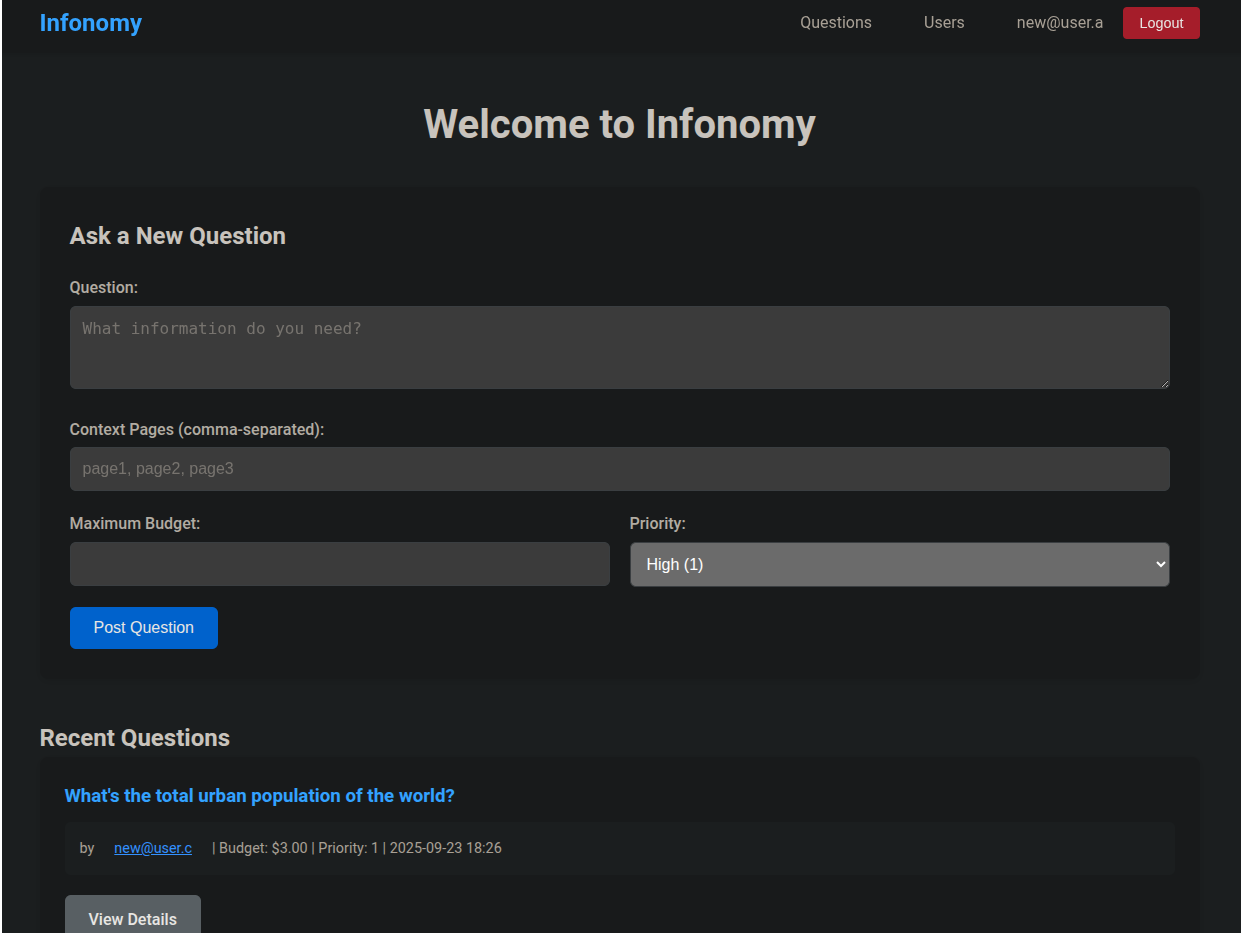
\includegraphics[width=0.9\linewidth]{figures/recursive-markets/infonomy_1.png}
    \caption{Posting a new question (\BuyerContext); viewing \BuyerContexts on the server}
    \label{fig:infonomy-1}
  \end{subfigure}

  \begin{subfigure}[b]{\columnwidth}
    \centering
    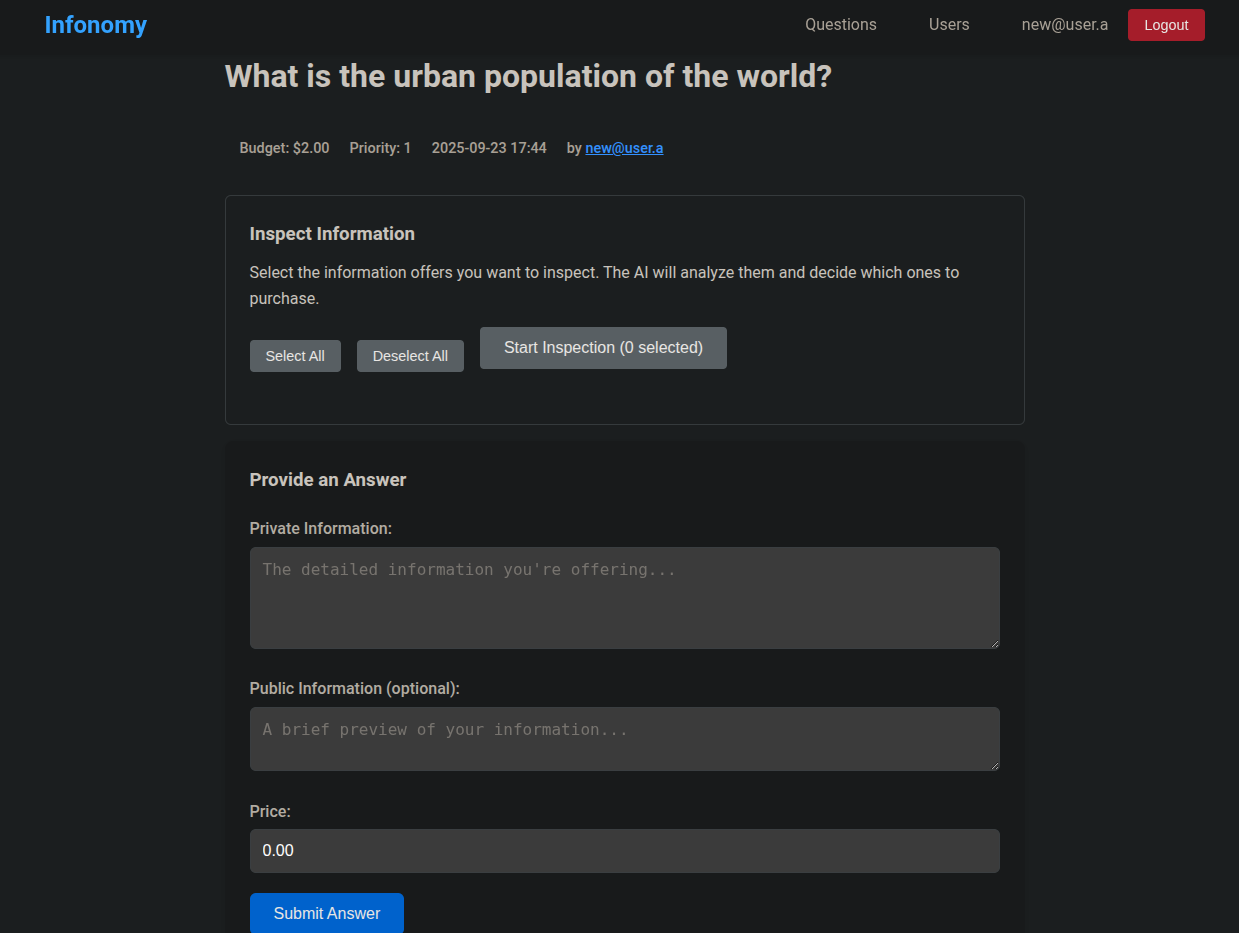
\includegraphics[width=0.9\linewidth]{figures/recursive-markets/infonomy_2.png}
    \caption{Posting an answer (\InfoOffer{}); initiating a recursive inspection}
    \label{fig:infonomy-2}
  \end{subfigure}

\end{figure}

\begin{figure}[htbp]
  \ContinuedFloat
  \centering
  \begin{subfigure}[b]{\columnwidth}
    \centering
    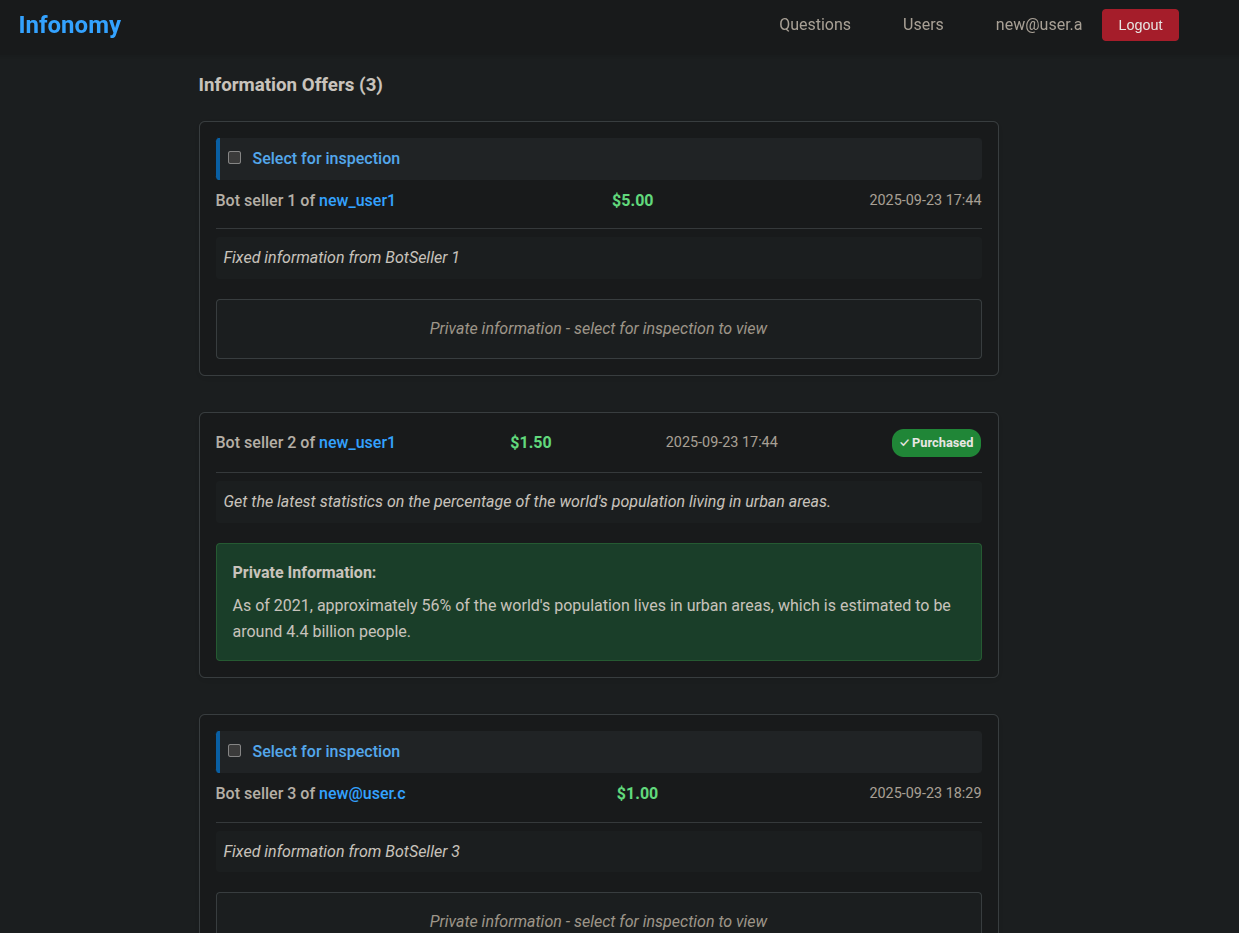
\includegraphics[width=0.9\linewidth]{figures/recursive-markets/infonomy_3.png}
    \caption{Inspecting and purchasing \InfoOffers{}; viewing purchased \InfoOffers{}}
    \label{fig:infonomy-3}
  \end{subfigure}

  \begin{subfigure}[b]{\columnwidth}
    \centering
    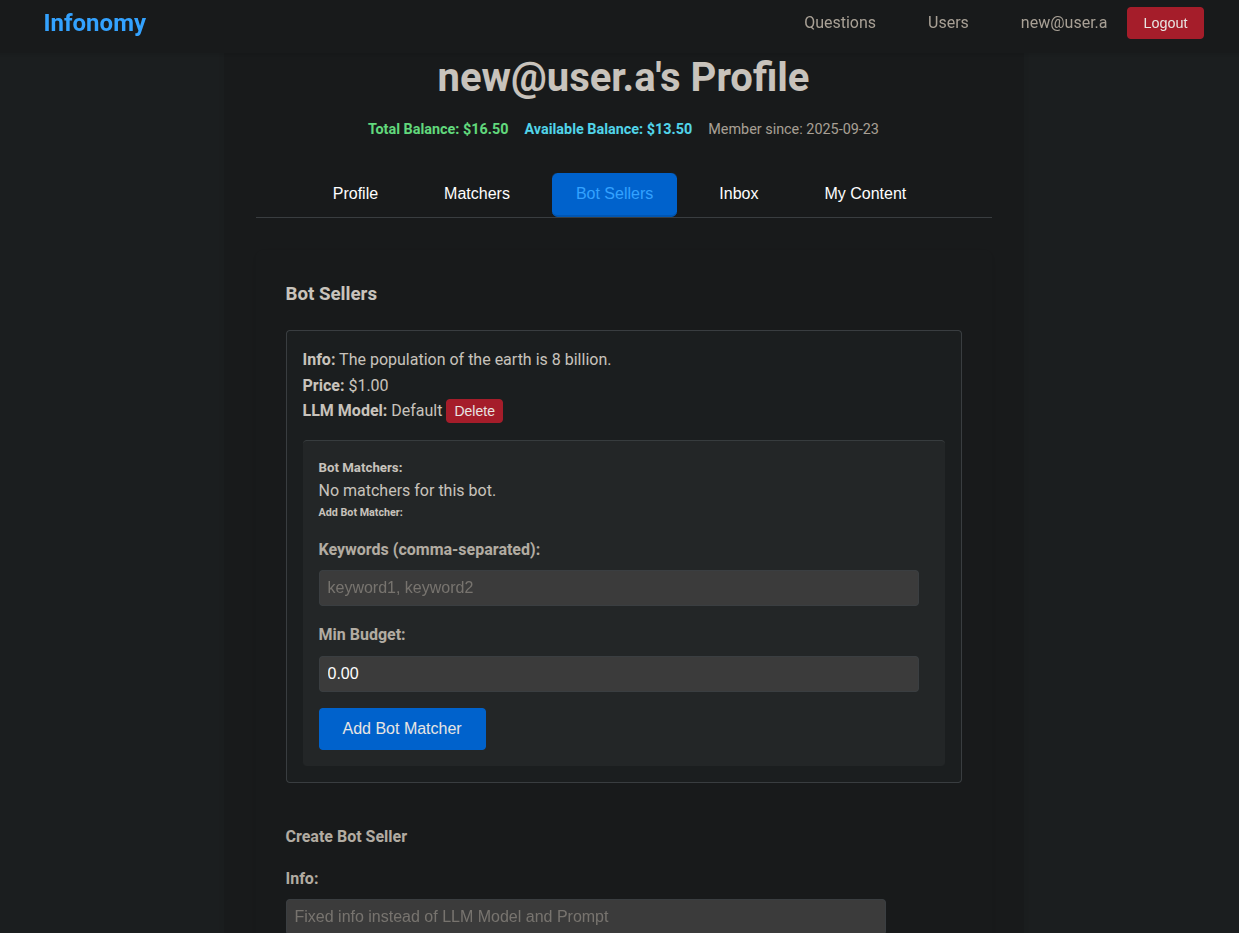
\includegraphics[width=0.9\linewidth]{figures/recursive-markets/infonomy_4.png}
    \caption{Bot sellers automatically answer recursive \BuyerContexts}
    \label{fig:infonomy-4}
  \end{subfigure}

  \caption{Screenshots from the \texttt{infonomy-server} platform}
  \label{fig:infonomy}
\end{figure}


A working implementation of an information market server implementing the Recursive Inspection Protocol is available at the \infonomy{} repository\footnote{\infonomyurl} -- some screenshots of the platform's GUI are shown in \Cref{fig:infonomy}. Many applications of such a server are immediate:

\begin{itemize}
\item \emph{Question \& Answer site} -- As presented, \infonomy{} can be seen as a Q \& A site with market incentives for answering questions.
\item \emph{Privatized product regulation} -- The \BuyerContexts{} might be names or links to products (the decision being ``should I buy?''), and the \InfoOffers{} could be inspection checks done by private labs, or customer reviews, which are now incentivized to be answerable to the customer.
\item \emph{Community Notes} -- In the spirit of well-known crowdsourced fact-checking systems such as Community Notes/Birdwatch \citeps{birdwatch2022}, we might use information markets as a ``comments section for the internet'', where \BuyerContexts{} would be links to webpages or social media posts (the decision being ``should I believe?'') and the \InfoOffers{} would be fact-checks or important context.
\item \emph{Reasoning in prediction markets} -- Forecasters on prediction markets may benefit from incentivizing the provision of information relevant to a forecast. One solution to this was given by \citets{conitzerPredictionMarketsMechanism2012}; another is to use \infonomy{}: where the \BuyerContexts{} are the questions being forecasted on (``What is the correct probability of this question?'') and the \InfoOffers{} are any relevant pieces of information.
\end{itemize}



\section{Future work}
\label{sec:so}

We have introduced a Bayesian framework for ``extrapolated volition'': i.e. to model a subjective buyer/rater's ``most fully informed'' score for the value of some piece of information. This allows us to design mechanisms for information markets (\cref{app:nonnaive}) as well as for supplying human feedback to AI models (\cref{sec:scoring}).

The ideal desideratum we would like a scalable oversight mechanism to satisfy is that it should incentivize the AI/information-seller to give the optimal information according to the information \emph{it} possesses: if the seller has information $K=(I_1,I_2,\dots)$, it should give information $I$ that optimizes\footnote{Naively one may think this means the AI should simply give $K$---realistically though, $K$ would be very large, reflecting the AI's entire knowledge and capabilities. Thus taking the cost of $K$ into account (assumed to be $\infty$ in \cref{sec:scoring}), that would certainly not be optimal.} $\mathbf{E}[U^1(I)|K=k]$. This would exactly describe the buyer's extrapolated volition: \emph{what would the buyer do if she were as smart as the AI?} Or we could say: this would exactly \emph{align} the AI or information-seller to our own values, while maintaining its superior information.

Unfortunately, our marginal value mechanism does not satisfy this hope. Take the following example.

\begin{example}
Suppose our decision problem is $\{0,1\}$ and:
\begin{itemize}
\item in our prior judgement, 0 is the better choice: $\mathbf{E}[U(0)]=1$, $\mathbf{E}[U(1)]=0$
\item  $I_1$ tells us 1 is better: $\mathbf{E}[U(0)|I_1]=0$, $\mathbf{E}[U(1)|I_1]=1$
\item  $I_2$ refutes $I_1$ and says 0 is better: $\mathbf{E}[U(0)|I_1,I_2]=1$ and $\mathbf{E}[U(1)|I_1,I_2]=0$
\item  $I_3$ refutes $I_2$ and says 1 is better: $\mathbf{E}[U(0)|I_1,I_2,I_3]=0$ and $\mathbf{E}[U(1)|I_1,I_2,I_3]=1$
\item with the full information, 1 is the better choice: $\mathbf{E}[U(0)|K]=0$, $\mathbf{E}[U(1)|K]=1$
\end{itemize}

But say $I_1$ and $I_2$ are cheap, while $p(I_3)=100$. Then the best information to reveal is $I_1$ --- but it won't be revealed, because $I_2$ will cheaply refute it while defending it with $I_3$ is too expensive. Thus instead we want to say that the agent can't give information \emph{so bad} that its shortfall exceeds its ``cost of defense'' (in this case, 100).

\end{example}

So while it is \emph{not} generally true that $x^1_*=\arg\max_{x^1}\mathbf{E}[U^1(x^1)|K]$, we may hope for a lower bound on ``how bad'' the equilibrium could possibly get, i.e. a result like $\mathbf{E}[U^1(x^1_*)|K]\ge \max_{x^1}\mathbf{E}[U^1(x^1)|K]-\mathcal{E}$ for some shortfall expression $\mathcal{E}$ that is some measure of the ``cost of defending the correct information''---and we may also use the expression for such a shortfall as a measure of how good a particular scalable oversight protocol is.


% We have introduced the \emph{recursive inspection protocol} as an information market mechanism for agents that are capable of ``inspecting and forgetting'' information, and provided a working implementation of the algorithm employing LLM agents. Our mechanism is optimal in a certain fundamental sense that accounts for the cost of obtaining information.

% The most promising direction for future work is to explore applications of this mechanism to \emph{scalable oversight} in AI alignment. Our mechanism may be seen as a formalization of Extrapolated Volition \citeps{yudkowskyCoherentExtrapolatedVolition2004}, which is informally described as the ``action an agent would prefer if it had all the relevant information''.
% \Cref{alg:rim} itself may be remniscient of scalable oversight proposals such as ``Humans Consulting HCH'' \citeps{christianoHCH}.

% More generally, one of the key limitations of currently widely-used alignment techniques such as reinforcement learning from human feedback (RLHF) is that they fundamentally rely on a human's ability to judge the correctness or value of a (potentially superhuman) AI's outputs \citeps{rlhflimits,burnsWeaktoStrongGeneralizationEliciting2024}. In other words, the AI is trained on the human supervisor's \emph{immediate, superficial} volition, rather than on her \emph{extrapolated volition} \citeps{yudkowskyCoherentExtrapolatedVolition2004}. In this context, our proposal may be used to augment a human rater's judgement of the AI's outputs with an information market, better reflecting her ``extrapolated volition''.

\include{chapters/scalable_oversight_benchmark}

\part{Eliciting Beliefs on Subjective Questions}
\chapter{Markets without Immediate Ground Truth}
\label{chap:subjective-intro}

\begin{drafttext}
Prediction markets and proper scoring rules ordinarily rely on an eventual
resolution. Yet many beliefs relevant to scientific reasoning, governance, and
AI oversight concern propositions whose truth is expensive, delayed, or not
captured by a fixed verification criterion. Information markets also face a
second problem: information is often valuable only in combination with other
information, so marginal contributions are not directly observable.

This part develops two complementary responses. Verification--falsification
games extend market elicitation to logical claims beyond simple verifiability or
falsifiability. Consistency checks evaluate a forecaster instantaneously by
searching for incoherence and arbitrage across related forecasts. A fuller
account of the connection to cooperative-game allocations and two-layer
information markets remains an explicit editorial task for the next draft.
\end{drafttext}

\chapter{Betting on What Is Neither Verifiable nor Falsifiable}
\label{chap:nonverifiable-betting}

\chapterprovenance{Adapted from ``Betting on what is neither verifiable nor
falsifiable'' by Abhimanyu Pallavi Sudhir and Long Tran-Thanh.}

\NewDocumentCommand{\Props}{}{\operatorname{Prop}}


%\newcommand{\ltt}[1]{{ \color{blue}[ltt:#1]}}
% \newcommand{\noop}[1]{}

\section*{Abstract}
Classical methods to elicit probabilities of events, such as proper scoring rules and prediction markets, are only useful when the events are either \emph{verifiable} (if true, will eventually be revealed as true) or \emph{falsifiable} (if false, will eventually be revealed as false). However, both probability theory and first-order logic allow for events/sentences that do not fit these criteria -- a simple example of such a sentence is ``all men are mortal''\todo{better example? e.g. will the US ever permanently annex Greenland?}. In this paper, we propose a mechanism to elicit probabilities on such sentences, by treating them as bets on the outcome of a ``verification-falsification game''. Our work thus acts as an alternative to the existing Garrabrant induction framework for logical uncertainty, and is related to concepts such as game semantics and Debate.\todo{last sentence too crude?}


\section{Introduction}

% important to elicit beliefs
%\emph{Incentivizing (human or AI) agents to truthfully report their beliefs} is a problem of central importance in both machine learning and economics\todo{cite something on proper scoring rules -- also should I explain why it's important?}. There are two classical approaches to this: \emph{proper scoring rules} (e.g. in logarithmic scoring, where an agent is given reward $\log(r)$ for reporting probability $r$ for a binary event which resolves True, its expected reward is maximized by reporting its true belief) and \emph{prediction markets} (to find an agent's subjective probability for the sentence ``Jeb Bush will win the 2028 election'', offer it a contingent asset that pays out \$1 if Jeb wins and \$0 otherwise -- the agent's fair price for the asset, at which it neither buys nor sells, may be taken to be its subjective probability).
\emph{Incentivizing (human or AI) agents to truthfully report their beliefs} is a problem of central importance in both machine learning and economics \cite{savageElicitationPersonalProbabilities1971,gneitingStrictlyProperScoring2007}. One standard approach to this is \emph{proper scoring rules}: e.g. in logarithmic scoring \cite{goodRationalDecisions1952}, an agent is given reward $\log(p)$ for reporting probability $p$ to a binary event which turns out to be true. Another approach is a \emph{prediction market} \cite{hansonLogarithmicMarketScoring2002, hansonCombinatorialInformationMarket2003, beygelzimerLearningPerformancePrediction2012, conitzerPredictionMarketsMechanism2012}: here, an asset contingent on the event is offered to the agent, and the agent's ``fair price'' (the price at which it neither buys nor sells), is its subjective probability -- for example, if you believe there is a 70\% chance of Jeb Bush winning the 2028 election, you will pay \$0.70 for the asset ``pays \$1 if Jeb wins; \$0 otherwise''.
%, and it is easy to see that the agent can maximize its expected reward under probability distribution $(p, 1-p)$ by reporting a probability of $p$

% scoring rules, prediction markets depend on ground truth
% easy to extend to VF
All of these mechanisms depend on the ground truth of the sentence being eventually revealed. At most, we can generalize them to \emph{verifiable sentences} (sentences whose ground truth will be revealed if they are true, e.g. ``Bob will eventually die'', verified by Bob dying) or \emph{falsifiable sentences} (sentences whose ground truth will be revealed if they are false, e.g. ``Bob will never die'', falsified by Bob dying) -- for the latter, we may pay the agent \$1 upfront, to be returned upon the sentence being falsified.

% fol and probability theory
% examples of such sentences
Although falsifiability occupies a central role in the imagination of philosophers \cite{thorntonKarlPopper2023}, a much wider class of sentences are treated in science and in common practice, and are allowed by first-order logic (FOL) and probability theory. In FOL, we may let $\Delta_0=\Sigma_0=\Pi_0$ denote sentences that will resolve in known time, $\Sigma_{n+1}$ denote sentences of the form $\exists x\ P(x)$ where $P(x)$ is $\Pi_n$, and $\Pi_{n+1}$ denote sentences of the form $\forall x\ P(x)$ where $P(x)$ is $\Sigma_n$. Thus verifiable sentences are $\Sigma_1$, and falsifiable sentences are $\Pi_1$, but all sentences further up the arithmetical hierarchy, $\Sigma_{n>1},\Pi_{n>1}$ are \emph{neither verifiable nor falsifiable} (non-VF)\todo{Similarly in probability theory, if we let $\{X_1,X_2,\dots\}$ be a set of base events which will be observed within finite time, then countable unions of subsequences $\bigcup_{i} X_{i_j}$ denote verifiable sentences (observing any true $X_i$ verifies it) while countable intersections $\bigcap_{i} X_{i_j}$ denote falsifiable sentences (observing any false $X_i$ falsifies it). But sentences higher up, e.g. $\bigcup_i\bigcap_j X_{f(i, j)}$ are non-VF.}. Examples of non-VF sentences:
\begin{itemize}
  \item ($\Pi_2$) ``all men are mortal'' ($\forall\,\mathrm{man}\,\exists t,\operatorname{dies}(\texttt{man}, t)$)
  \item ($\Sigma_2$) ``The US will eventually permanently annex Greenland'' ($\exists t,\forall s>t,\,\texttt{greenland\_in\_us\_at\_time}(s)$)
  \item ($\Pi_3$) ``Long-run GDP growth will be expontential with rate 2\%'' ($\forall\varepsilon>0,\exists t, \forall s>t, \,|\left(\texttt{GDP}(t)/\texttt{GDP(0)}\right)^{1/t}-1.02|<\varepsilon$)
\end{itemize}

In all of these cases, there is no source of ground truth that lets us resolve the question with certainty: verifying ``all men are mortal'' would need checking an infinite number of men who will ever be born; falsifying it would require finding an immortal man, but proving him to be immortal will take infinite time. Yet these are all very common sentences, which we may find it useful to have a probability estimate on.

There are two common ways that market-creators attempt to work around this limitation in practice\footnote{this can be attested by a brief skim through the front pages of popular forecasting platforms such as Polymarket and Manifold Markets}:
\begin{itemize}
\item asking about \emph{finite-horizon} versions of non-VF sentences (e.g. ``Greenland will be annexed and remain part of the US until at least 2100''), or
\item asking whether the sentence will be \emph{proven} (either via formal proofs or appealing to the authority of ``credible sources'').
\end{itemize}
The pitfalls of the first method are explained in Section~\ref{vf/sec:impossible}; the most refined example of the second method is \emph{Garrabrant induction} \cite{garrabrantLogicalInduction2020}, described in Section~\ref{vf/sec:related}.

We propose a new framework for eliciting probabilities on non-VF sentences: we allow agents to bid for the opportunity of playing the \emph{verification-falsification game} for that sentence, and take the value of the bid to be their implied probability for that sentence. {There are limitations to our mechanism, such as when one side of the game is much easier to play than the other, and we outline some ideas on how these may be overcome.}


\subsection{Related work}
\label{vf/sec:related}

\textbf{Logical uncertainty.} Our work may equivalently be understood as a formalism for \emph{logical uncertainty} (see \cite{halpernReasoningUncertaintySecond2017} for a summary of work in the area), i.e. the problem of assigning probabilities to mathematical sentences in some language $\mathcal{L}$ (which could be a language of FOL sentences). The most relevant work in this domain is \emph{Garrabrant induction} \cite{garrabrantLogicalInduction2020}, which constructs a prediction market for each mathematical sentence that pays off when it is proven by a theorem-enumerator for some theory $\mathcal{T}$ over $\mathcal{L}$.\footnote{to avoid simply being a prediction market for the provability of a sentence, they use a special accounting measure for agent wealths based on ``propositionally consistent worlds'' -- e.g. fixing the combined price of $P$ and $\lnot P$ at \$1 -- which allows them to extend this framework to sentences independent of $\mathcal{T}$.}

There are two limitations of this framework for our purposes. First: while mathematical theories can easily prove non-VF sentences (e.g. $\forall x,\exists y>x,\,\texttt{prime}(y)$) there is no analogous theory in the real world that we are aware of (``observation'' only proves VF sentences, as discussed). Second: it is philosophically unsatisfying to have probabilities for logical sentences be completely dependent on a mathematical theory, and change when the theory is strengthened or weakened (e.g. by the addition of a G\"odel sentence).

Logical uncertainty has also been discussed in the Bounded Rationality literature e.g. in \cite{halpernAlgorithmicRationalityGame2014,halpernDontWantThink2011,oesterheldTheoryBoundedInductive2023}; however this has typically focused on toy examples based on VF sentences, e.g. betting on the trillionth digit of $\pi$, etc.

\textbf{Game semantics.} The \emph{verification-falsification game} we use is from Hintikka's \emph{game semantics} \cite{hintikkaGameTheoreticSemantics1997}, which we will discuss in Section~\ref{vf/sec:framework}. Game semantics has since been expanded into the field of \emph{computability logic} \cite{japaridzeBeginningWasGame2009,japaridzeSurveyComputabilityLogic2015}, which may be the most natural setting to formulate some of our more speculative ideas about probability theory, described in Sec~\ref{vf/sec:conclusion}.

\textbf{Debate.} AI Debate \cite{irvingAISafetyDebate2018} considers sentences $P$ that can be expressed like $\exists x_1\ \forall x_2\ \dots \exists x_n,H(x_1,\dots x_n)$ (more generally any $\Sigma_n$ or $\Pi_n$ form in $H$) where $H$ is some ``human-computable function'', and argues that AIs can be trained to answer such questions correctly via \emph{debate} judged by a human\footnote{in particular, supervised learning can train an AI to learn to answer $\Delta_0$ questions, and reinforcement learning can train an AI to learn to answer $\Sigma_1$ questions}. This is quite similar to our setting, and debate is analogous to the verification-falsification game, except that physical ground truth is replaced by human-computability (or polynomial-computability as they hypothesize). We hope our work can serve as a valuable intuition pump for debate.

\NewDocumentCommand{\VFPAPERProblem}{}{\mathbf{Pr}}
\NewDocumentCommand{\VFPAPERProb}{O{}m}{%
  \mathbf{Pr}%
  \IfValueT{#1}{^{#1}}%
  \left[#2\right]%
}

\textbf{AI Forecasting.} There has recently been a surge of interest in AI forecasters \cite{zouForecastingFutureWorld2022, schoeneggerLargeLanguageModel2023,yanAutoCastEnhancingWorld2023, halawiApproachingHumanLevelForecasting2024a, schoeneggerWisdomSiliconCrowd2024} -- in particular, recent works such as \cite{sudhirConsistencyChecksLanguage2024} have investigated the \emph{propositional consistency} of AI forecasters, i.e. whether the probabilities they give satisfy basic rules of probability theory like $\VFPAPERProb{P}+\VFPAPERProb{\lnot P}=1$. Similarly our work can be understood as asking how we can incentivize or evaluate forecasters respecting the ``continuity of probability'' rules $\VFPAPERProb{\bigcup P_i}=\lim_{n\to\infty}\bigcup_{i<n}\VFPAPERProb{P_i}$ and $\VFPAPERProb{\bigcap P_i}=\lim_{n\to\infty}\bigcap_{i<n}\VFPAPERProb{P_i}$.

\section{Impossibility theorem}
\label{vf/sec:impossible}

One apparent solution may be to approximate FOL sentences with long finite horizons -- i.e. approximate $\exists x,\forall y, P(x,y)$ with a bounded quantification $\exists x<G,\forall y<G, P(x,y)$ for some large $G$, which is a $\Delta_0$ sentence as it can be determined by enumerating $G^2$ tuples. One might also consider a sequence of such bounded quantification ``approaching'' the FOL sentence, e.g. consider the asset that on day $t$ is equal to (can be exchanged for) $\exists x< t,\forall y< t, P(x,y)$. A simple counter-example to this approach is: $\exists x,\forall y,x\ge y$, illustrated in Fig~\ref{fig:checkerboard}: for any finite $G$, the corresponding bounded quantification is true (take $x=G$), but the sentence is false.

\begin{figure}
  \centering
  \input{figures/nonvf/checkerboard2}
  \caption{Infinite checkerboard with the square $(x,y)$ shaded iff $x\ge y$. Then $\exists x,\forall y, x\ge y$ says that there is an infinite black column, which is false, but ``true on every finite window''.}
  \label{fig:checkerboard}
\end{figure}

Theorem~\ref{thm:nogo} shows there is no general mechanism to give a proper scoring rule or an equivalent asset for any non-VF sentence:

\begin{definition}[Asset and scoring mechanisms]
  An asset mechanism is a computable real-valued function $v:\Nats\times\Props\to\Reals$ such that $\lim_{t\to\infty}v(t,P)=1$ if $P$ and $0$ if $\lnot P$. Let $s:[0,1]\to\Reals$ be a proper scoring rule e.g. $s(p)=\log(p)$. A scoring mechanism for proper scoring rule $s$ is a computable real-valued function $\sigma:\Nats\times\Props\times[0,1]\to\Reals$ such that $\lim_{t\to\infty}\sigma(t,P,p)=\{s(p)\text{ if }P\text{ else }s(1-p)\}$.
  \label{def:mechanisms}
\end{definition}

\begin{theorem}[Impossibility theorem]
  If $\Props$ is the set of FOL sentences, then there does not exist either an asset mechanism nor a scoring mechanism.
  \label{thm:nogo}
\end{theorem}
\begin{proof}
  The statements $\lim_{t\to\infty}v(t,P)=1$ and $\lim_{t\to\infty}\sigma(t,P,p)=s(p)$ are both $\Pi_3$ for any $P, p$; thus for them to be equivalent to $P$ for all $P$ would violate Tarski's theorem.
\end{proof}

\section{Ranged VF games}
\label{vf/sec:framework}

In this paper, we propose a game-theoretic solution motivated by the following intuition. If you believe that ``all men are mortal'', then you should agree to the following bet: I can choose the name of any man, and you must be able to give the year by which he will be dead. If you succeed, you win the bet; if you don't, I win. This is formally analogous to the classic Verification-Falsification (VF) game from \cite{hintikkaGameTheoreticSemantics1997}, described in Def~\ref{def:vfgame}.

\RenewDocumentCommand{\finset}{}{\operatorname{finset}}

\begin{definition}[Verification-Falsification game]
  To each FOL sentence $P$ we associate a sequential game between two players, the ``Verifier'' ($V$) and the ``Falsifier'' ($F$). If $P$ is $\Delta_0$, then $V$ or $F$ win \$1 if $P$ is true or false respectively. Else if $P$ is $\Sigma_n$, then $V$ goes first and if $P$ is $\Pi_n$, then $F$ goes first. The first player chooses $x\in\Nats$ as their move, and the game proceeds as the VF game for $P[x]$ (i.e. the leading bound variable substituted with $x$). Some variations:
  \begin{itemize}
  \item (\emph{ranged}) Instead of picking $x\in\Nats$ as its move, each player picks a finite set $S\in\finset\Nats$ as its move and the game proceeds as $P[S]$ , i.e. $\exists x\in S,P[x]$ if $P$ is $\Sigma_n$ or $\forall x\in S,P[x]$ if $P$ is $\Pi_n$. This eventually terminates when all the quantifications have become bounded, i.e. the sentence is $\Delta_0$.
  \item (\emph{favorable}) One of the players is ``favored'': they are allowed to go back to any earlier stage of the game, change it moves, and continue from there, as many times as it wants. This is the ``game with backward moves'' from \cite{bonnayPreuvesJeuxSemantiques2004,boyerProofTruth2012}, and has the property that if the favored player's position is provable, they have an obvious computable winning strategy (a depth-first search with backtracking).
  \end{itemize}
  \label{def:vfgame}
\end{definition}

The \emph{ranged} VF game is original to us, and is what we use: you might believe that all men are mortal but have a probability distribution on the year any one of them will die, rather than knowing the exact date with certainty.

Observe that player policies have type $\pi:\Props\to\finset\Nats$. We may denote the $\Delta_0$ sentence produced after playing the game through as $P[\pi_V,\pi_F]$. Although the game is traditionally defined for logical sentences, it is easy tro see how this extends to probabilistic events:

\begin{definition}[FOL algebra]
  Let $\Delta_0=\Sigma_0=\Pi_0=\{B_1,B_2,\dots\}$ consist of a set algebra of base events which will be observed within finite time; $\Sigma_{n+1}$ consist of all events of the form $\bigcup_{i}X_i$ where $X_i$ is $\Pi_n$ and $\Pi_{n+1}$ consist of all events of the form $\bigcap_{i}X_i$ where $X_i$ is $\Sigma_n$. Then we will call $\Delta_0\cup\bigcup\Sigma_n\bigcup\Pi_n$ an ``FOL algebra'' over $\Delta_0$, and it is a subset of the $\sigma$-algebra generated by $\Delta_0$.
  \label{def:probfol}
\end{definition}

We will continue to freely write $\bigcup_{i}X_i$ and $\bigcap_{i}X_i$ in the logical notation $\exists i,X_i$ and $\forall i,X_i$. We may easily speak of probabilities $\VFPAPERProb{P}$ of sentences in the FOL algebra by defining a probability distribution on the base set algebra. Then we have the following result\footnote{this can be seen as a generalization of the classic statement from game semantics that the verifier or falsifier has a winning strategy if and only if the sentence is true or false respectively}:

\begin{theorem}[Value of ranged VF game]
  Assume a FOL algebra with a probability distribution $\VFPAPERProblem$ defined on it, and let $P$ be a sentence in this FOL algebra. Then $\VFPAPERProb{P}$ is bounded between the guaranteed value of the game for the verifier and 1 minus the guaranteed value of the game for the falsifier:

  \begin{equation*}
    \sup_{\pi_V}\inf_{\pi_F}\VFPAPERProb{P[\pi_V,\pi_F]} \le
    \VFPAPERProb{P} \le
    \inf_{\pi_F}\sup_{\pi_V}\VFPAPERProb{P[\pi_V,\pi_F]}
  \end{equation*}
  (where the $\sup$ and $\inf$ are taken over $\Props\to\finset\Nats$) We will denote each side of the inequality as $\VFPAPERProb[-]{P}$ and $\VFPAPERProb[+]{P}$ respectively.
  \label{thm:supinf}
\end{theorem}
\begin{proof}
We prove this by induction on the degree of $P$. Suppose the theorem is true for $P$ up to $\Sigma_n,\Pi_n$. Then take some event $P:=\forall x, P(x)$ where each $P(x)\in\Sigma_n$:

\begin{align*}
  \VFPAPERProb{P}
  &=\VFPAPERProb{\bigcap_{x\in\Nats}P(x)}\\
  % &\text{by continuity of probability:}\\
  &=\inf_{S\in\finset\Nats}\VFPAPERProb{\bigcap_{x\in S}{P(x)}}\\
  % &\text{by the inductive hypothesis:}\\
  &\ge
  \inf_{S\in\finset\Nats}
    \sup_{\pi_V}\inf_{\pi_F}\VFPAPERProb{
      \left(\cap_{x\in S}{P(x)}\right)[\pi_V,\pi_F]
    }\\
  % &\text{by the max-min inequality \cite{boydConvexOptimization2004}:}\\
  &\ge \sup_{\pi_V}\inf_{S\in\finset\Nats}\inf_{\pi_F}\VFPAPERProb{
    \left(\cap_{x\in S}{P(x)}\right)[\pi_V,\pi_F]
  }\\
\end{align*}

(where we have successively applied continuity of probability, the inductive hypothesis and the max-min inequality) Now note that $\left(\cap_{x\in S}{P(x)}\right)[\pi_V,\pi_F]=P[S][\pi_V,\pi_F]$, which is equivalent to $P[\pi_V,\pi'_F]$ where $\pi'_F$ is identical to $\pi_F$ except on $P$, where $\pi'_F(P)=S$. Thus:
\begin{equation*}
  \VFPAPERProb{P}\ge \sup_{\pi_V}\inf_{\pi'_F}\VFPAPERProb{
    P[\pi_V,\pi'_F]
  }
\end{equation*}

Which completes the first half of the inequality. The proof for the $P\in\Sigma_{n+1}$ case is identical, and the other half of the inequality is immediate from applying the first half to $\lnot P$.

\end{proof}

\newenvironment{hproof}{%
  \renewcommand{\proofname}{Proof sketch}\proof}{\endproof}

% \begin{corollary}[Ranged favorable non-VF game]
%   In the $V$-favourable ranged game, the verifier can guarantee a value of $\VFPAPERProb[+]{P}$. In the $F$-favourable ranged game, the falsifier can guarantee a value of $1-\VFPAPERProb[-]{P}$.
%   \label{thm:supinff}
% \end{corollary}
% \begin{hproof}
% In the $V$-favorable ranged game,
% \end{hproof}


Several elicitation mechanisms are now immediate:

\textbf{Bidding to play.} Agents bid to play as either the verifier or falsifier of a ranged VF game for $P$. The highest bidders for each side are chosen to play against each other, and their bids are taken as estimates of the probability of $P$ and $\lnot P$. Note that the market-maker does not have to take a loss: even though this may be a negative-sum game because of potential computational costs, the total prices will still add up to at least \$1 because otherwise one of the players could just bid to take both sides and win a guaranteed total \$1.

\textbf{Double auctions.} However, it is possible for agents to overestimate their winnings and drive the total price above \$1, and this also does not give a way for agents to bid down the price of one position. We can solve this by selling multiple games via a double-auction with an order book where buy offers for the Falsifier position at price $q$ are interpreted as sell orders for the Verifier position at price $1-q$ and matched to buy orders for the Verifier position at price $p\ge 1-q$.

\textbf{Subsidized markets.} Alternatively, we may simply run one high-stakes Verification-Falsification game, retaining bidding for selecting players, but base probabilities on a separate betting market for the outcome of the game. It is possible here that the best players are not selected (e.g. due to independently wealthy players outbidding them), but an advantage is that these markets can be subsidized with arbitrary scoring rules\footnote{See \cite{hansonLogarithmicMarketScoring2002} for an introduction to market scoring rules}; traditional methods to integrate scoring rule based market makers such as \cite{agrawalUnifiedFrameworkDynamic2011, chakrabortyPriceEvolutionContinuous2015} do not work for us, as they require the market-maker to take the opposite side of every trade, which for us will require having the market-maker actively play the game.

\textbf{Training AI forecasters.} We can get our probability estimates from an AI instead of the market, by training an ``estimating agent'' $\alpha:\Props\to\finset\Nats\times[0,1]$ which outputs both a move and an estimate of its reward. The agent may then earn a combined reward for winning the game and for placing an accurate forecast. The most natural architecture for such a forecaster would be a transformer which takes input in natural or formal language and gives a sequence of integers as its output. %To be precise: the learning problem is a multi-agent Markov Decision Process (MDP) with initial state $P\in\Props$, actions $(S,b)\in\finset\Nats\times[0,1]$, transition function $P'=P[S]$ and reward functions for the final state $\vec{R}(P)=(\theta(P),1-\theta(P))\text{ if }P\in\Delta_0\text{ else }0$ where $\theta$ is the ground truth resolver for $\Delta_0$.
% Better, we can compute rewards at each step by the agent's own next estimate of the value (and have that next estimate be deducted from the next reward), to allow for more efficient credit assignment -- Algorithm~\ref{alg:train} shows a simple self-play training loop implementing this.

% \NewDocumentCommand{\VFs}{}{\{\Sigma,\Pi\}}
% \algnewcommand{\LeftComment}[1]{\(\triangleright\) #1}
% \NewDocumentCommand{\dataset}{}{\mathcal{D}}

% \begin{algorithm}[tb]
% \caption{Training an AI forecaster for non-VF sentences}
% \label{alg:train}
% \begin{algorithmic}

% \Procedure{TrainingLoop}{}

% \State \textbf{input }Dataset $\dataset\subseteq\Props$
% \State \textbf{input }Ground truth resolver $r:\Delta_0\to\bools$
% \State\LeftComment{$\VFs$ encodes which side the player is playing as}
% \State Initialize agent $\alpha_\theta:\Props\times\VFs\to\finset\Nats\times[0,1]$

% \For{$t<N_{\text{epochs}}$}
% \For{$P\in\dataset$}
% \State $n=\deg(P)$\Comment{i.e. $P$ is $\Sigma_n$ or $\Pi_n$}
% \For{$i\in [n,\dots 0]$}

% \State $\kappa=\Sigma\text{ if }P\in\Sigma_i\text{ else }\Pi$
% \State $S,b\gets \alpha_\theta(P,\kappa)$\Comment{get action $S$ and estimate $b$}
% \State

% \EndFor
% \EndFor{}
% \EndFor{}

% \EndProcedure
% \end{algorithmic}
% \end{algorithm}


\section{Computational limitations}
\label{vf/sec:complexity}

There are two practical limitations of our work:
\begin{enumerate}
  \item Each player's move can be a finite set of arbitrary size, and the player is incentivized to play larger and larger finite sets. In particular, the final $\Delta_0$ sentence will be a disjunctive normal form over a very large number of $\Delta_0$ sentences, and getting the ground truth evaluations for all of them may take a long time (or cost a lot in computation).
  \item We have not considered computational costs of playing the VF game; the $\sup$ and $\inf$ in Theorem~\ref{thm:supinf} are over all possible policies, even non-computable ones. In particular, the computational difficulty of playing for each side might be \emph{asymmetric}.
\end{enumerate}

For the first, we may charge a transaction cost proportional to the cardinality of the chosen move $S$ to incentivize agents to be selective in choosing the members of $S$ -- alternatively we may add a common discounting factor to the reward that would also disincentivize agents from choosing moves that would take a long time for their opponent to respond to. In the market mechanisms, we can also allow the agents to sell their place in the game to another agent at any point in time, so they do not need to wait for ground truth to be revealed to collect their reward.

\NewDocumentCommand{\Ack}{}{\mathcal{A}}

The second is more serious: a classic example in game semantics \cite{solovievVerifierFalsifierGamesRestrictions2022} is the sentence $\exists x,\forall y,y\le\Ack(x)$ where $\Ack$ is the Ackermann function, and the class of policies is limited to primitive recursive functions (i.e. all other functions are infinitely expensive to play). Although this sentence is ``obviously'' false, $V$ can pick any $S$, and $F$ will be unable to win because the Ackermann function grows faster than all primitive recursive functions. In our case, it is apparent that if we took the $\sup_{\pi_V}$ and $\inf_{\pi_F}$ in Theorem~\ref{thm:supinf} to be over primitive recursive functions only, the lower and upper bounds are both $1$, though $\VFPAPERProb{P}$ should be 0 as $P$ is false.

\NewDocumentCommand{\Compcl}{}{\mathcal{C}}

One solution may come from the ``favourable'' games mentioned in Def~\ref{def:vfgame}. In the example above, the falsifier has a winning strategy in the $F$-favourable game by indefinitely trying larger and larger integers as its move until it wins.

More generally, if we restrict the class of allowable policies to some $\Compcl\subset(\Props\to\finset\Nats)$, the $V$-favorable (respectively $F$-favourable) game still allows the $\sup$ (respectively $\inf$) to be taken over all of $\Props\to\finset\Nats$, as that player can simply enumerate each possible strategy. In general, we may play both the $F$-favorable and $V$-favorable games, and the range between the values of these games contains the range in Theorem~\ref{thm:supinf}:

\begin{align}
&\sup_{\pi_V\in\Compcl}\inf_{\pi_F}\VFPAPERProb{P[\pi_V,\pi_F]}\nonumber\\
&\le
\sup_{\pi_V}\inf_{\pi_F}\VFPAPERProb{P[\pi_V,\pi_F]}\nonumber\\
&\le
\VFPAPERProb{P}\label{eq:bounds}\\
&\le
\inf_{\pi_F}\sup_{\pi_V}\VFPAPERProb{P[\pi_V,\pi_F]}\nonumber\\
&\le
\inf_{\pi_F\in\Compcl}\sup_{\pi_V}\VFPAPERProb{P[\pi_V,\pi_F]}\nonumber
\end{align}

Other approaches might be inspired by the Debate literature, for example \cite{brown-cohenScalableAISafety2023} introduces a version of the Debate protocol called ``Doubly-efficient debate'', where the honest strategy wins ``even when the debater is computationally unbounded''. Extending this to VF games should be a topic of future research.

It remains unclear how much of a problem these computational limitations will be in practice.

\section{Discussion and future work}
\label{vf/sec:conclusion}

We have presented the ``ranged Verification-Falsification game'' and demonstrated that eliciting agents' values for playing this game provides useful bounds on the probability of an FOL sentence. Although usually applied to mathematical logic, FOL can also express sentences about some empirical universe, even if the process that generates empirical truth is probabilistic in nature. Our mechanism stands as an alternative framework to \cite{garrabrantLogicalInduction2020} for logical uncertainty, as well as the first mechanism to elicit probabilities on non-VF sentences from markets and AI models outside of a strict logical context. There are three other potential implications of our work deserving of attention.

\textbf{Formal logic.} Our work may provide a new approach to measuring the strength of a mathematical theory: in the $V$-favourable VF game, a formal proof from a mathematical theory gives a computable winning strategy \cite{bonnayPreuvesJeuxSemantiques2004, boyerProofTruth2012}; we my then consider the maximum wealth that can be acquired by an agent that only trades and plays in accordance with a theory, and regard this as a measure of the strength of the theory.

\textbf{Eliciting latent knowledge.} Though we have used ``non-VF'' to refer specifically to FOL sentences, these are not the only sentences whose truth cannot be ascertained by ground truth. Take e.g. the sentence ``Bob did the crime''. This will not in itself be revealed by any future empirical observation, but may ``correlate'' with (provide information on) other, more directly valuable sentences like ``if Bob is jailed, fewer burglaries will happen'', ``evidence of Bob's wrongdoings will be found'' and ``if you hire Bob, you may find some office supplies missing''. One may say that these useful sentences are all correlated, and therefore ``Bob did the crime'' is a useful fiction constructed to capture the signal in the noisy data, a \emph{variable in the latent space}. The problem of eliciting information on such sentences has been discussed in e.g. \cite{tailcalledLatentVariablesPrediction2023, baillonBayesianMarketsElicit2017, baillonSimpleBetsElicit2021}, and directly addresses the problem of \emph{interpretability} in AI safety \cite{christianoElicitingLatentKnowledge2021}. We hope our work may serve as an entrypoint towards solving this much more ambitious goal.

\NewDocumentCommand{\toc}{}{\to_{\Compcl}}

\textbf{Alternative formulations of probability theory.} It would be interesting to study what the elicited probabilities in these mechanisms actually approach in the limit, more precisely than the bounds in Equation~\ref{eq:bounds}, e.g. when training AI forecasters (where $\Compcl$ would be the class of functions approximable by a neural network) or with a double auction containing every computable function in some class (e.g. those computable in polynomial-time) included as a trader by eventual enumeration. This would induce some ``distribution'' over the FOL algebra, which would \emph{not} be a probability distribution in the traditional sense (would not satisfy continuity of probability), as this would contradict Theorem~\ref{thm:nogo}. Instead we might consider an alternate definition of a $\sigma$-algebra $\mathcal{F}$ which is required to be closed only under unions and intersections of \emph{computable sequences}, i.e. replacing the countable union axiom with ``$\psi:\Nats\toc\mathcal{F}\implies\bigcup_i\psi(i)\in\mathcal{F}$'' (where $\Compcl$ is some class of computable functions) and adopting a suitable generalized notion of probability measure on this algebra. Possibly relevant work to this end includes: quantifier algebras \cite{cwooQuantifierAlgebra2013}, Shafer \& Vovk's game-theoretic formulation of probability theory \cite{shaferProbabilityFinanceIts2005, shaferGameTheoreticFoundationsProbability2019} and Japaridze's ``Computability Logic'' \cite{japaridzeBeginningWasGame2009, japaridzeSurveyComputabilityLogic2015}.

\chapter{Consistency Checks for Language Model Forecasters}
\label{chap:consistency-checks}

\chapterprovenance{Adapted from ``Consistency Checks for Language Model
Forecasters'' by Daniel Paleka, Abhimanyu Pallavi Sudhir, Alejandro Alvarez,
Vineeth Bhat, Adam Shen, Evan Wang, and Florian Tram\`er.}

%\newcommand{\rebuttal}[1]{\textcolor{red}{#1}}
\newcommand{\rebuttal}[1]{#1}
\newcommand{\rebuttaldeleted}[1]{}
\section*{Abstract}
Forecasting is a task that is difficult to evaluate: the ground truth can only be known in the future. Recent work showing LLM forecasters rapidly approaching human-level performance begs the question: how can we benchmark and evaluate these forecasters \textit{instantaneously}? Following the consistency check framework, we measure the performance of forecasters in terms of the consistency of their predictions on different logically-related questions. We propose a new, general consistency metric based on  \textit{arbitrage}: for example, if a forecasting AI illogically predicts that both the Democratic and Republican parties have 60\% probability of winning the 2024 US presidential election, an arbitrageur can trade against the forecaster's predictions and make a profit. We build an automated evaluation system that generates a set of base questions, instantiates consistency checks from these questions, elicits the predictions of the forecaster, and measures the consistency of the predictions. We then build a standard, proper-scoring-rule forecasting benchmark, and show that our (instantaneous) consistency metrics correlate with LLM forecasters' ground truth Brier scores (which are only known in the future). We also release a consistency benchmark that resolves in 2028, providing a long-term evaluation tool for forecasting.

\section{Introduction}

\emph{Prediction markets} are markets that pay out contingent on an event. For a market such as ``\$1 if Jeb Bush is elected President in 2028'', the price reflects the ``market estimate'' for the probability of that event. Prediction markets are a promising tool for aggregating information from disparate sources to arrive at the most correct possible belief after taking into account all relevant information \citep{arrowPromisePredictionMarkets2008, hansonLogarithmicMarketScoring2002}.


Until 2024, LLM forecasters generally performed poorly relative to human forecasters \citep{zouForecastingFutureWorld2022, schoeneggerLargeLanguageModel2023}.
However, recent works \citep{halawiApproachingHumanLevelForecasting2024, schoeneggerWisdomSiliconCrowd2024,safeai2024forecasters} suggest that LLM-based forecasters can rival human forecasts on forecasting websites such as Metaculus, PredictIt, and Manifold Markets.
%\citet{halawiApproachingHumanLevelForecasting2024} achieve this via retrieval-augmented generation (RAG) and fine-tuning, while \cite{schoeneggerWisdomSiliconCrowd2024} obtain consensus from a crowd of LLM forecasters.
%\manyuunimp{perhaps mention https://www.lesswrong.com/posts/uGkRcHqatmPkvpGLq/contra-papers-claiming-superhuman-ai-forecasting and references therein, including the Hendrycks paper people were criticizing}
%There is also an ongoing ``Humans vs Bots'' competition underway on Manifold Markets \cite{manifoldHumanBotsForecasting2024}
%\todo{idk if we want to cite the Scott Alexander blog post?}.

A key question emerges: \emph{once LLM forecasters are better than human ones, how can we efficiently evaluate their predictions?}
In particular, long-term forecasting questions are very important for decision-making \citep{tetlock2024longrange, lukemuehlhauserHowFeasibleLongrange2019}, and finding ground truth for evaluation in such contexts is infeasible by virtue of the questions resolving far in the future.

One approach, proposed by \citet{esmwcc}, is that even when we cannot evaluate the \emph{correctness} of LLM decisions, we can evaluate their \emph{logical consistency}.
For example, if an LLM forecaster gives probabilities 0.5 and 0.7 to ``Will Trump be elected US president?'' and ``Will someone other than Trump be elected US president?'', this is necessarily inconsistent.
\citet{esmwcc} demonstrated that GPT-4 and GPT-3.5-turbo, when asked one-sentence forecasting questions, were inconsistent on simple logical checks such as negation.

%\newpage

%\manyu{@dpaleka: describe our exact novelty against Fluri. Maybe also: (1) a bit longer of a spiel about consistency, training for consistency etc. (2) specific research questions e.g. does it correlate with ground truth, what if we just arbitraged the forecasts, etc.}
\begin{figure}[h]
    \begin{minipage}{0.55\textwidth}
    % First figure content
    \centering
    \vspace{-10pt}
    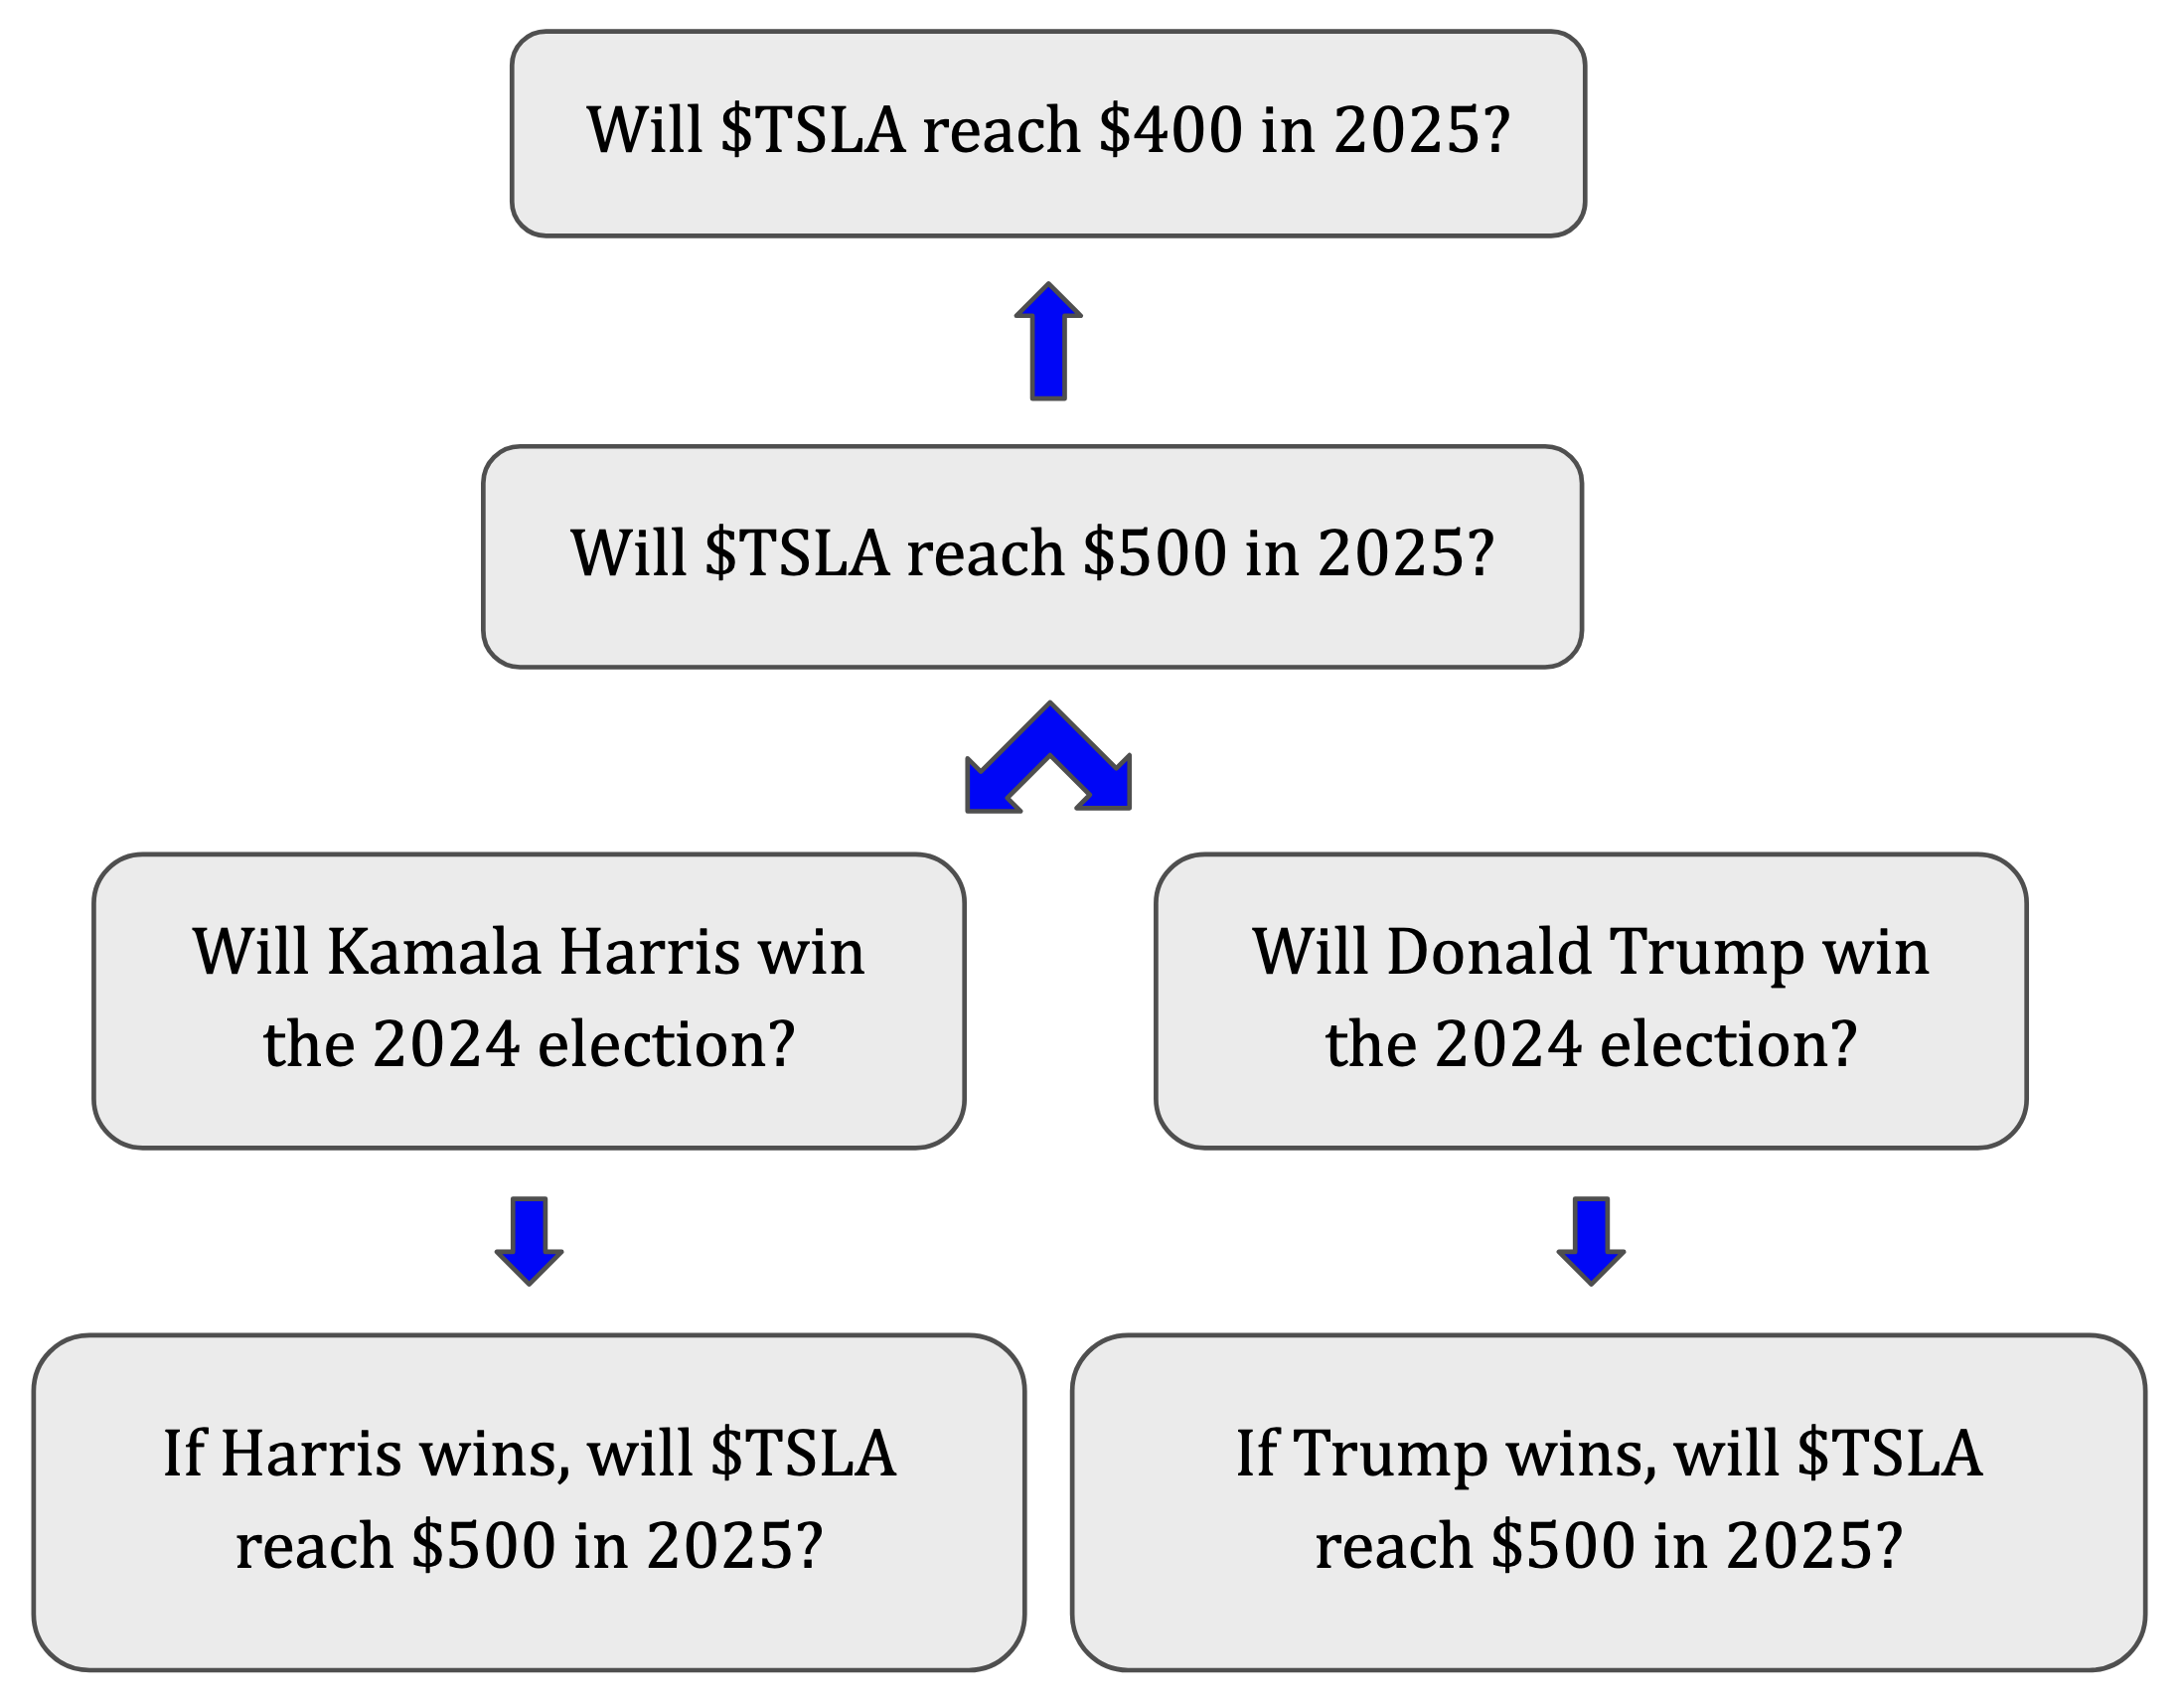
\includegraphics[width=\textwidth]{figures/consistency/fig1_short.png}
    \captionsetup{width=0.95\textwidth}
    \caption{
        Examples of
        %the \ConsequenceChecker{} and \ExpectedEvidenceChecker{}
        consistency check questions generated from the same question about Tesla stock reaching \$500 in 2025. The pipeline in \Cref{cfc/sec:pipeline} generates questions and evaluates a forecaster's consistency with respect to them.
    }
    \end{minipage}
    \hfill
    \begin{minipage}{0.44\textwidth}
    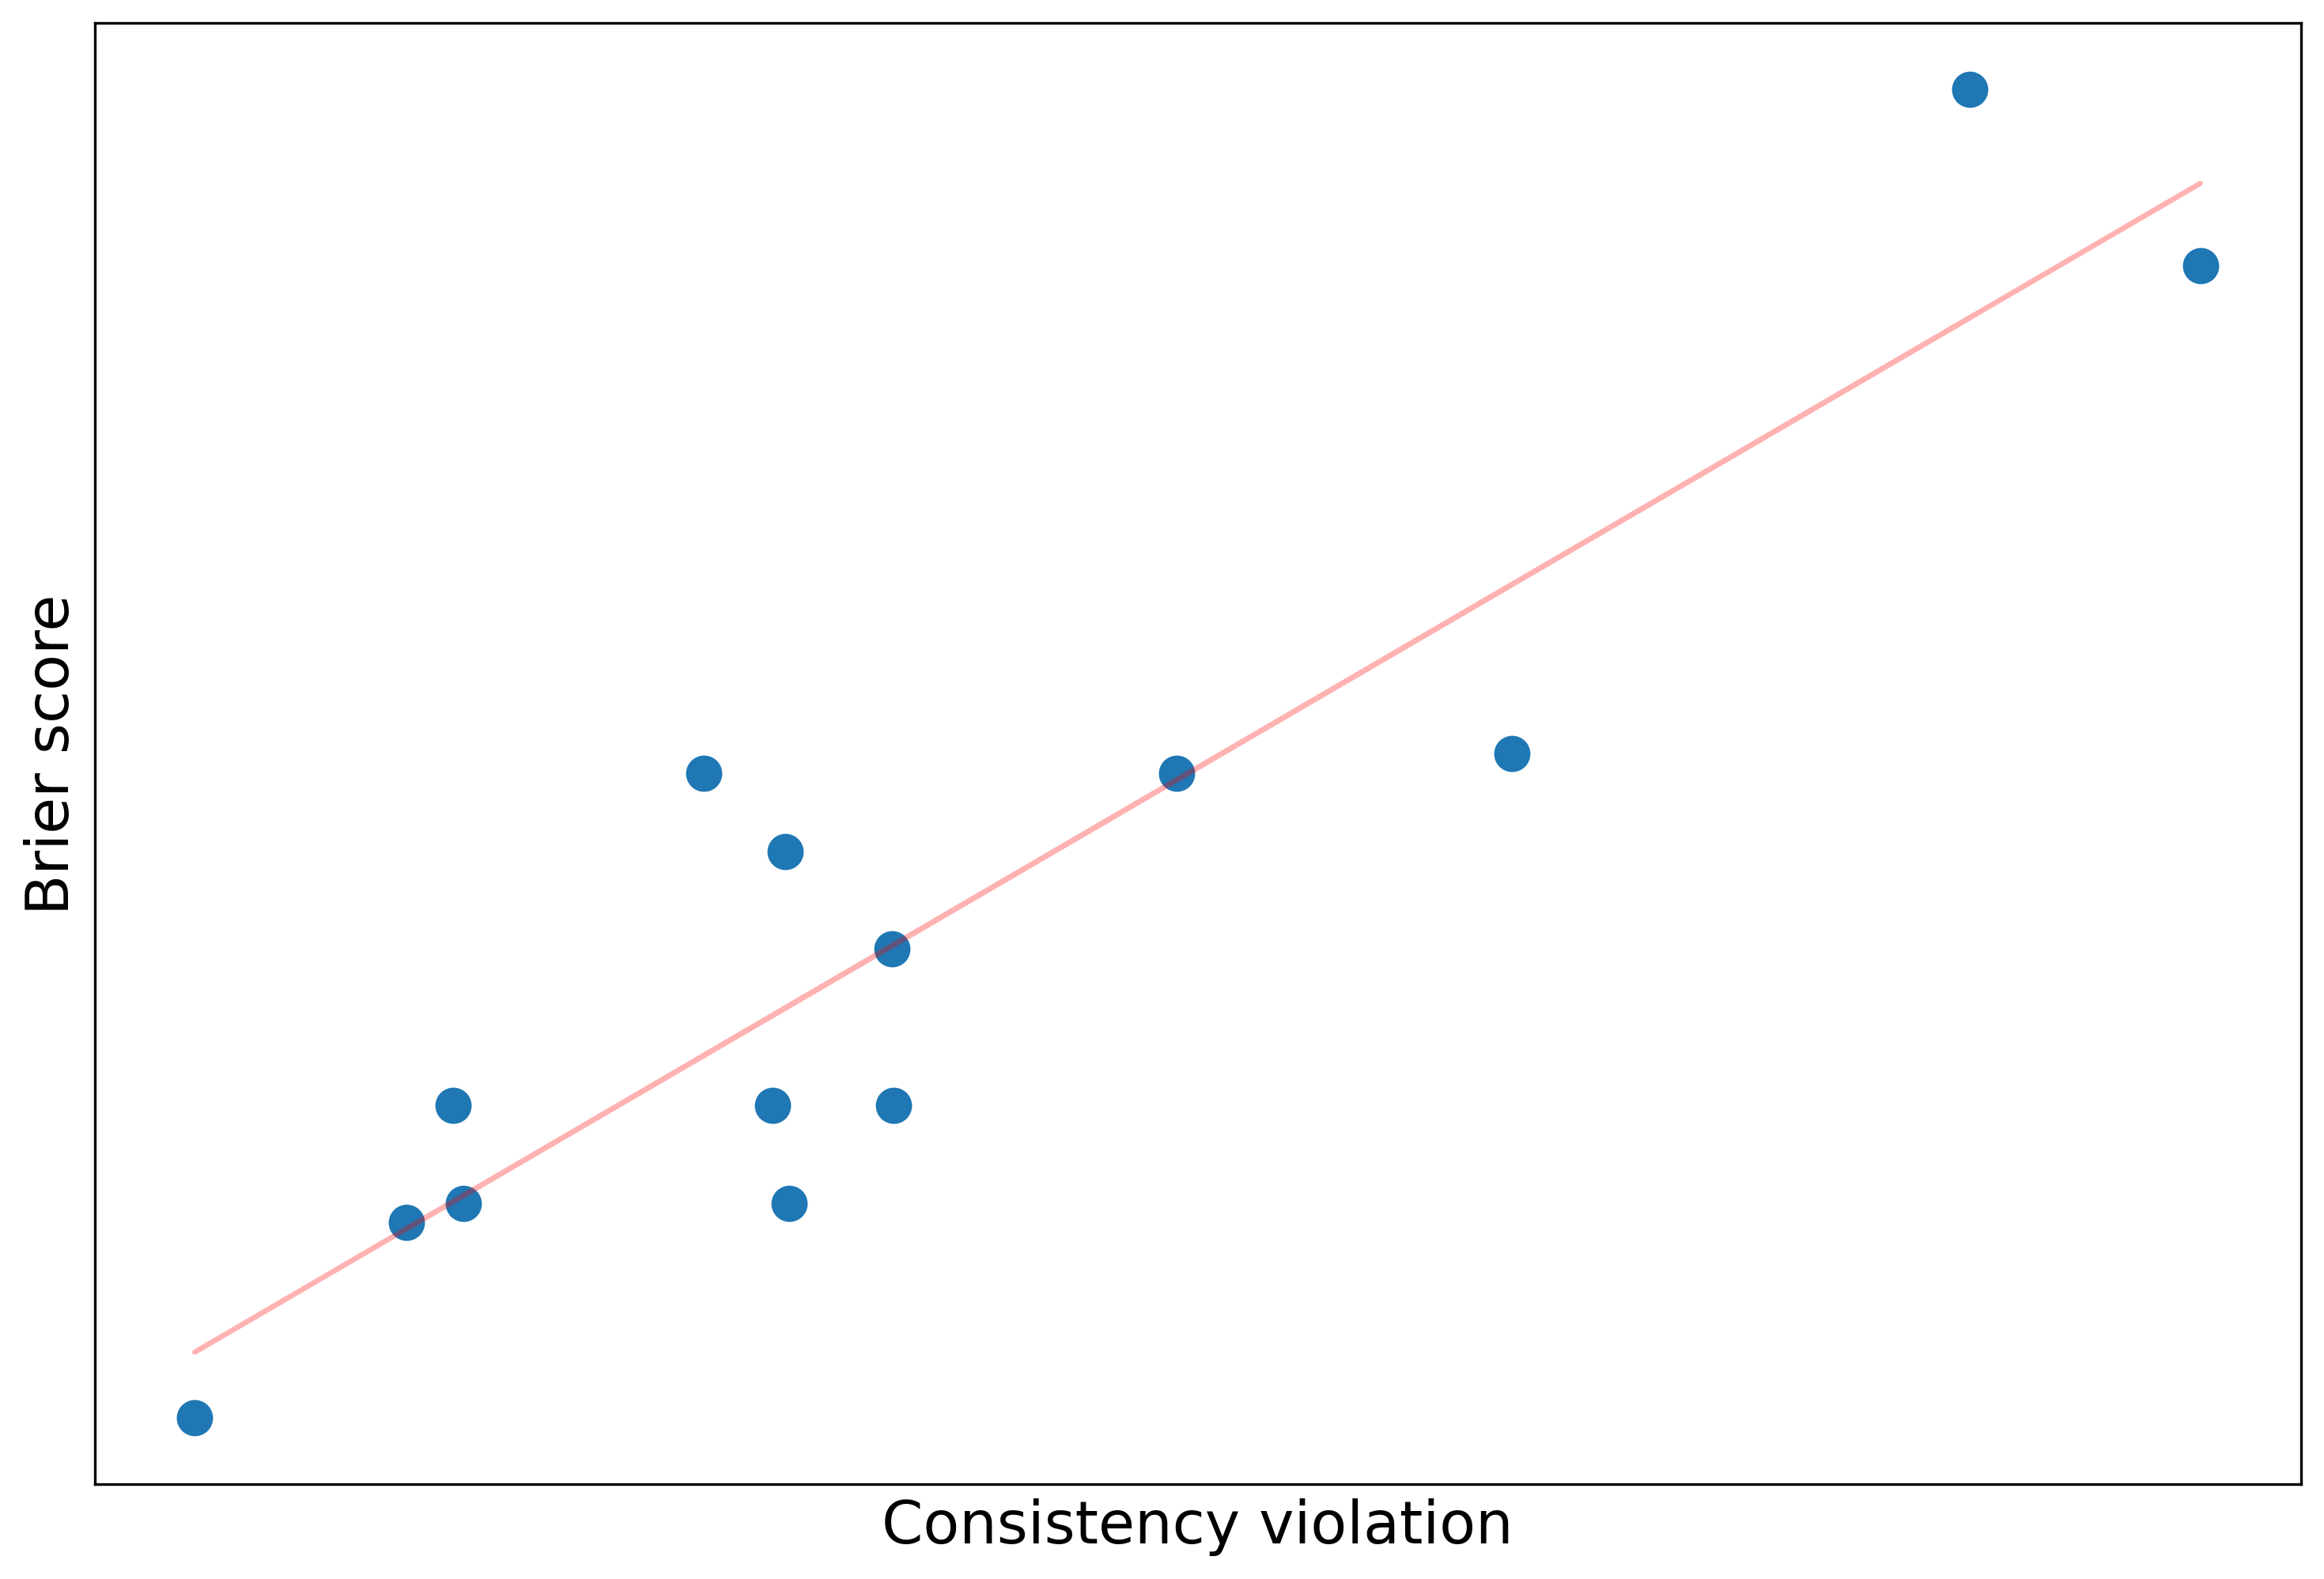
\includegraphics[width=\textwidth]{figures/consistency/CondChecker_vs_avg_brier_score_default_avg_violation_scraped_preview.png}
    \captionsetup{width=0.95\textwidth}
    \caption{
        The consistency violation scores on certain checks such as \CondChecker{} give signal about true forecasting performance over a range of forecasters, as described in \Cref{cfc/sec:results}.
    }
    \end{minipage}
    \label{fig:overview}
\end{figure}

\begin{table*}[hbtp]
\centering
\caption{Consistency checks used in our paper and the corresponding logical consistency conditions.}
\vspace{5pt}
\label{tab:consistency_checks}
\begin{tabular}{l p{0.65\linewidth}}
\toprule
\textbf{Name} &
\textbf{Condition ($\CCheck$)}
\\ \midrule
\NegChecker &
$\Forecaster(P)+\Forecaster(\lnot P)=1$
\\ \midrule
\begin{tabular}{@{}l@{}} \ParaphraseChecker\\ $\Relation(P,Q):=P\iff Q$\end{tabular} &
$\Forecaster(P)=\Forecaster(Q)$
\\ \midrule
\begin{tabular}{@{}l@{}} \ConsequenceChecker\\ $\Relation(P,Q):=P\implies Q$\end{tabular} &
$\Forecaster(P)\le\Forecaster(Q)$
\\ \midrule
\AndOrChecker &
$\Forecaster(P)+\Forecaster(Q)=\Forecaster(P\lor Q)+\Forecaster(P\land Q)$
\\ \midrule
\AndChecker &
$\max(\Forecaster(P)+\Forecaster(Q)-1, 0) \le \Forecaster(P\land Q) \le \min(\Forecaster(P),\Forecaster(Q))$
\\ \midrule
\OrChecker &
$\max(\Forecaster(P),\Forecaster(Q))\le\Forecaster(P\lor Q)\le\min(1,\Forecaster(P)+\Forecaster(Q))$
\\ \midrule
\ButChecker &
$\Forecaster(P\lor Q)=\Forecaster(P)+\Forecaster(\lnot P\land Q)$
\\ \midrule
\CondChecker &
$\Forecaster(P)\Forecaster(Q|P)=\Forecaster(P\land Q)$
\\ \midrule
\CondCondChecker &
$\Forecaster(P)\Forecaster(Q|P)\Forecaster(R|P\land Q) =\Forecaster(P\land Q\land R)$
\\ \midrule
\ExpectedEvidenceChecker &
$\Forecaster(P)=\Forecaster(P|Q)\Forecaster(Q)+\Forecaster(P|\lnot Q)(1-\Forecaster(Q))$
\\ \bottomrule
\end{tabular}
\end{table*}

%\include{tikzfig1}

Our contributions in this work are as follows:

\textbf{1) Principled metrics for consistency.~}
In \Cref{cfc/sec:background}, we introduce a theoretical framework for measuring consistency violations of binary forecasts, based on two metrics: an \emph{arbitrage metric}, based on market arbitrage, and a \emph{frequentist metric}, based on hypothesis testing. We apply these metrics to 10 different logical consistency rules (see \Cref{tab:consistency_checks}):
\NegChecker{}, \ParaphraseChecker{},  \ConsequenceChecker{}, \AndOrChecker{}, \AndChecker{}, \OrChecker{}, \ButChecker{}, \CondChecker{}, \CondCondChecker{} and \ExpectedEvidenceChecker{}.
%The metrics are introduced in \Cref{cfc/sec:consistency-checks-intro} and \Cref{cfc/app:arbitrage,cfc/app:frequentist-metric}.
%We leave training forecasters to be consistent with these metrics as an exciting direction for future work.

\textbf{2) A consistency evaluation pipeline for binary forecasters.~}
In \Cref{cfc/sec:pipeline}, we introduce a \emph{consistency evaluation pipeline} for LLM forecasters.
We create two forecasting datasets with known ground truth resolutions: one scraped from prediction markets, and one synthetically generated from news articles.
Both datasets include only events that happen past the training data cutoff of all forecasters we test, and resolve before September 2024.
We then generate tuples of forecasting questions satisfying logical consistency rules with associated consistency metrics.

%\evanunimp{keywords or categories/tags? -- I think keywords makes more sense in the intro (vin)}

\textbf{3) Consistency correlates with ground truth forecasting performance.}
Our consistency metrics are novel performance metrics for forecasters that can be computed right away, no matter the time horizon.
Of course, forecasters could also be evaluated using \emph{backtesting}, asking past questions with known ground truth resolutions.
Yet, backtesting LLM forecasters can be challenging if we do not have clear information about the models' training data contents. Moreover, there may be new types of questions that we want to evaluate forecasters on, for which we do not have appropriate past results (e.g., questions related to pandemics before 2020).
It is thus natural to ask:
\emph{can consistency metrics tell us anything about future forecasting performance?}

In \Cref{cfc/sec:results}, we show that for all forecasters we test, our consistency metrics correlate positively with forecasting performance (as measured by the Brier score) on both our benchmark datasets.
The correlation varies across consistency checks, with some logical checks (e.g., consistency of conditional probabilities) having over $R=0.9$ correlation with forecasting performance, while other logical tests provide little signal.
We \rebuttal{hypothesise that this analysis can extend} to smarter forecasters and longer time horizons, to provide instantaneous feedback on forecaster performance.

\textbf{4) Scaling inference-time compute can improve consistency for some logical checks, but fails to generalize.}
Since we find that consistency correlates with forecasting performance, it is natural to ask whether we can improve forecasters by making them more consistent. Unfortunately, we find that natural ways of improving consistency tend to overfit to specific consistency checks and do not generalize.

Specifically, we design \CFCaster{}: a forecaster that ``patches'' some base forecaster's output by generating logically related questions and ``arbitraging'' the base forecaster's forecasts for these related questions against each other.
In Section~\ref{cfc/sec:cfcaster} and \Cref{cfc/app:cfcaster}, we show that \CFCaster{} improves consistency on checks that we optimize against, but this improvement does not generalize to other held-out consistency checks, nor does it improve the actual forecasting performance.

\textbf{5) A long-horizon forecasting consistency benchmark.}
%In \Cref{cfc/sec:results} and \Cref{cfc/app:synthetic-questions-2028},
We create a long-horizon benchmark of 3,000 consistency checks for forecasts resolving in 2028. Our benchmark spans questions on various topics for which we will have no ground truth for more than three years, and thus serves as a nice testing ground for advanced LLM forecasters.


We release the full code \footnote{\url{https://github.com/dpaleka/consistency-forecasting}} and the datasets \footnote{\url{https://huggingface.co/datasets/dpaleka/ccflmf}} used in the paper.

%\towrite{list of experiments (list of forecasters tested, ground truth correlation, CF description, metaculus bot) -- or something.}

\section{A theoretical framework for forecasting consistency}
\label{cfc/sec:background}
\label{cfc/sec:forecasting}

%\section{Forecasting}
%\todo{I don't think there should be a subsection with just notation}

%\towrite{Background on Forecasting as a task @manyu.}

\begin{notation*}
    Let $\ForecastingQuestions$ denote the set of forecasting questions we are interested in, $\Resolutions$ denote the set of possible outcomes/resolutions for an individual questions.
    \rebuttal{
    In this paper, we focus on $\ForecastingQuestions$ as a set of binary forecasting questions, so $\Resolutions=\bools$.
    %and $\Forecasts=\probs$.
    }
    %and $\Forecasts$ denote the set of probability distributions on $\Resolutions$.
    A \emph{Forecaster} is then a map $\Forecaster:\ForecastingQuestions\to\probs$.
    One special forecaster is the ground truth resolutions $\Resolution:\ForecastingQuestions\to\Resolutions$, \rebuttal{returning $1$ and $0$ probability for $\bools$, respectively.}

    For conditional questions that can resolve to $\none$, we also have optional resolutions $\ResolutionsOpt:=\Resolutions\cup\{\none\}=\boolsopt$.
    We focus on binary questions following \cite{halawiApproachingHumanLevelForecasting2024}.
    \rebuttal{Our methods can in principle be extended to study consistency between general probability distributions in forecasting, such as the ones discussed in \citet{gooenScorableFunctionsFormat2024}.}
     %\manyuunimp{and because eliciting other probability distributions from LLMs is difficult (see the work of \citet{gooenScorableFunctionsFormat2024} for some work in this direction).}
     %i.e. Other questions types could involve a continuous value (what is the average temperate of New York in June 2025) or Multiple Choice (who will be the MVP of the NBA Championships in 2025?)  It is computationally intensive or intractable to test most consistency metrics with these types of questions.  However, multiple choice questions, can be subdivided into several binary questions, which is done in our set.  For example:  Will Lebron James by MVP in 2025; Will Kevin Durant be MVP in 2025...
\end{notation*}

\subsection{Consistency checks and inconsistency metrics}
\label{cfc/sec:consistency-checks-intro}

In line with \cite{esmwcc}, a consistency check is conceptualized as a pair of n-ary relations: \rebuttal{$\Relation:\ForecastingQuestions^n\to\bools$ in question space, $\CCheck:\probs^n\to\bools$ in forecast space, and a predicate for $\Forecaster$ such that $\Relation(x_1,\dots x_n)\implies\CCheck(\Forecaster(x_1), \dots \Forecaster(x_n))$.}
In particular, this assertion must be satisfied by all feasible $\Resolution$, and also any ``correct'' forecasts generated by a world model that accurately accounts for aleatoric uncertainty.
Violation of consistency is measured by some violation metric $\Violation:\probs^n\to\Reals$ which must satisfy $\Violation(\Forecaster(x_1),\dots\Forecaster(x_n))=0\iff\CCheck(\Forecaster(x_1),\dots\Forecaster(x_n))$.
%
For example, intuitively, the ``negation'' check \NegChecker{} is given by \rebuttal{the relation $\Relation(x_1,x_2) := x_1=\lnot x_2$ on questions, and the relation $\CCheck(\Forecaster(x_1), \Forecaster(x_2)) := \Forecaster(x_1)+\Forecaster(x_2) \approx 1$ on forecasts.}
The full table of the consistency checks we use is given in Appendix~\ref{cfc/app:checks}.

Improving upon \cite{esmwcc}, we derive $\Violation$
%(and therefore $\CCheck$)
from $\Relation$ in a principled way,
handling all types of logical consistency checks simultaneously.
We introduce two new \emph{inconsistency metrics}: the \emph{arbitrage metric} and the \emph{frequentist metric} for measuring logical inconsistency in probabilistic forecasts.

\subsubsubsection{Arbitrage metric}
\label{cfc/sec:arbitrage}

\NewDocumentCommand{\score}{m}{\ensuremath{s\left(#1\right)}}
\NewDocumentCommand{\consp}{}{p}
\NewDocumentCommand{\argmaxmax}{}{\mathop{(\argmax,\max)}}

The arbitrage metric is conceptualized as the minimum profit that an arbitrageur can be guaranteed making bets against the forecaster's predictions. More precisely: suppose that the forecaster's probabilities $\Forecaster(x_1),\dots\Forecaster(x_n)$ were prices offered by a logarithmic market maker \footnote{
A \emph{logarithmic market maker} with subsidy $w$ is a market maker who adjusts prices in response to trades such that the trader's reward for moving the probability of a true-resolving sentence from $p_0$ to $p'$ is $w\log p'-w\log p_0$.
%\rebuttaldeleted{Manifold Markets uses such a procedure.}
For further background on scoring rules and the associated market makers, see Appendix~\ref{cfc/app:arbitrage}, \rebuttal{\cite{berg2009hanson},}
or \cite{hansonLogarithmicMarketScoring2002}.
}  with market subsidy parameter \$1.
If these probabilities are inconsistent, then there are prices $p_1,\dots p_n$ that an arbitrageur could bring to the market such that it is guaranteed to make a profit against the market-maker, no matter the outcome of each question. We \rebuttal{define} $\Violation(\Forecaster(x_1),\dots\Forecaster(x_n))$ \rebuttal{as the maximum achievable} ``minimum profit'' that the arbitrageur can guarantee by choosing appropriate $p_1,\dots p_n$. We further denote by $\Arbitrageur(\Forecaster(x_1),\dots\Forecaster(x_n))$ the set of prices $p_1,\dots p_n$ that maximize the minimum profit:
\ft{math is hard to parse, just rewrite}
%This can also be interpreted as the ``minimum number of bits of information lost to inconsistency''.
%
\begin{equation}
\resizebox{.95\hsize}{!}{$\displaystyle
    \argmaxmax_{\consp\in[0,1]^n} \min_{\omega\in\Omega} \sum_{i=1}^n \left(\log{\consp_i}-\log{\Forecaster(x_i)}\right)\Indicator{\omega(i)=\top} + \left(\log{(1-\consp_i)}-\log{(1-\Forecaster(x_i))}\right)\Indicator{\omega(i)=\bot}$}
    \label{eq:arbitrage__}
\end{equation}
%
Here $\Omega:=\{\omega\in\ResolutionsOpt^n\mid\Relation(\omega)\}$ is the set of all possible consistent resolutions of this tuple. A more general version of ~\ref{eq:arbitrage__} is given in Appendix~\ref{cfc/app:arbitrage}, along with specific worked-out examples of the arbitrage metric for each consistency check, and details on how we compute it; as an example, the arbitrage metric for the Negation Check can be derived exactly (Appendix~\ref{apps:arbitrage-neg}):
%
\begin{equation*}
\begin{split}
    \Violation(\Forecaster(x),\Forecaster(\lnot x))=-2\log\left(\sqrt{\Forecaster(x)(1-\Forecaster(\lnot x))}+\sqrt{(1-\Forecaster(x))\Forecaster(\lnot x)}\right)
\end{split}
\end{equation*}
%
% \begin{definition}[Arbitrage-based Violation Metric]
%     Let $\Relation:\ForecastingQuestions^n\to\bools$ be an n-ary relation such that $\Relation(\Resolution(x_1), \dots \Resolution(x_n))$ is satisfied by the ground-truth resolutions $\Resolution:\ForecastingQuestions\to\Resolutions$ for all tuples $(x_1,\dots x_n)$. \footnote{This is well-defined because resolutions can be taken as a subset $\Resolutions\subseteq\ForecastingQuestions$, by treating them as forecasting questions that always resolve to themselves by definition. For example, the forecasting question $\top$ is always worth \$1 and the forecasting question $\bot$ is always worth \$0.} Let $s:\ForecastingQuestions\times\Resolutions\times[0,1]\to\Reals$ be a proper scoring rule that gives the score earned based on the probability assigned to the true resolution, e.g. $s(x,\Resolution,p(\Resolution))=\log p(\Resolution)$. Let $(x_1,\dots x_n)\in\ForecastingQuestions^n$ be a question tuple, and denote $\ResolutionsVec:=\{\resolutionvec\in\ResolutionsOpt^n\mid\Relation(\resolutionvec)\}$ the set of possible consistent resolutions (including $\none$ resolutions) of this tuple. Then for forecasts $(\Forecaster(x_1),\dots\Forecaster(x_n))$ the arbitraged forecasts $\Arbitrageur(\Forecaster(x_1),\dots\Forecaster(x_n))=(p_1\dots p_n)$ and the minimum guaranteed profit of the arbitrageur $\Violation(\Forecaster(x_1),\dots\Forecaster(x_n))$ are given by:
%
%     \begin{equation}
%         \argmaxmax_{\consp\in\Forecasts^n}
%         \min_{\resolutionvec\in\ResolutionsVec}
%         \sum_{i=1}^n
%         %\sum_{\Resolution\in\Resolutions}
%         \score{x_i, \resolutionvec_i, p_i(\resolutionvec_i)}
%         - \score{x_i, \resolutionvec_i, \Forecaster(x_i)(\resolutionvec_i)}%\Indicator{\omega_i=\Resolution}
%         \label{eq:arbitrage}
%     \end{equation}
%     Where by convention, any score on a resolution $\resolutionvec_i=\none$ is taken to be 0.
%     \label{def:arbitrage}
% \end{definition}
%
% Definition~\ref{def:arbitrage} is presented in full generality: $\consp$ and $\Forecaster(x_i)$ here are \emph{probability distributions} on $\Resolutions$. Breaking it down: each $\score{x_i, \resolutionvec_i, p_i(\resolutionvec_i)}- \score{x_i, \resolutionvec_i, \Forecaster(x_i)(\resolutionvec_i)}$ gives the arbitrageur's profit on the market for question $x_i$, given that it resolves $\resolutionvec_i$. The profit is summed across all markets in the tuple, and then minimized over all consistent worlds; this minimum is maximized across all possible arbitrageur bets.
%
% It is helpful to explicitly state Eq~\ref{eq:arbitrage} in the case of binary forecasting questions, as follows.
%
% \begin{equation}
%     \argmaxmax_{\consp\in[0,1]^n} \min_{\omega\in\Omega} \sum_{i=1}^n \left(\score{\consp_i}-\score{\Forecaster(x_i)}\right)\Indicator{\omega(i)=\top} + \left(\score{1-\consp_i}-\score{1-\Forecaster(x_i)}\right)\Indicator{\omega(i)=\bot}
%     \label{eq:arbitrage_}
% \end{equation}

% Appendix~\ref{cfc/app:arbitrage} includes specific worked-out examples of the arbitrage metric for each consistency check, and details on how we compute it; as an example, the arbitrage metric for the Negation Check can be derived exactly (Appendix~\ref{apps:arbitrage-neg}):


To illustrate: $\Violation(0.5,0.6)\approx 0.01$, $\Violation(0.5,0.51)\approx 10^{-4}$.
The metric is more sensitive to violations for probabilities very close to $0$ or $1$, due to the logarithmic market maker.
% TODO examples of this here
In our evals, for all types of checks, we say that a sampled check does not pass if $\Violation \ge 0.01$.
\rebuttal{We have to pick some hyperparameter as an inconsistency threshold; we set it to correspond} to
giving 110\% probability in total to the events of Republican and Democratic parties winning the US presidential election.

\subsubsubsection{Frequentist metric}
\label{subcfc/sec:frequentist-metric}

We also compute a different, \emph{frequentist} consistency metric. Consider a Monte Carlo forecaster that samples a world model $n$ times, and for any event, returns the fraction of samples in which the event occurs. The frequentist metric is the number of standard deviations a given tuple forecast is off from the mean Monte Carlo forecast, scaled to be independent of $n$. We say that a consistency violation happened if the number of standard deviations away from the mean of the null is at least as in the $(0.5, 0.6)$ case described in \Cref{cfc/sec:arbitrage}. The full description is given in \Cref{cfc/app:frequentist-metric}.
%\adamunimp{we should say what we picked as sigma = 0.05 here?}.\dpaleka{no,wit's confusing enough as it is}


\subsubsubsection{Intuition on consistency metrics}

Our metrics address two major obstacle with measuring inconsistency: \emph{tolerance to noise} and \emph{principled aggregation of inconsistency scores}.

\textbf{Tolerance to noise.}
In the standard Bayesian setting, beliefs are either consistent or not: there either is a Dutch book (a way to bet against the forecaster's beliefs to get infinite profit) or the probabilities are perfectly consistent.
In practice, an forecaster's beliefs (even on the same question) are never perfectly consistent across runs. If an election model has a presidential candidate at 48\% with one random seed and 50\% on the other, this is not a reason to discard it as completely flawed. Hence, instead of a binary measure of consistency, our metrics increase smoothly with inconsistency.

\textbf{Principled aggregation and comparison of inconsistency scores.}
\cite{esmwcc} developed a set of inconsistency checks, used an ad-hoc metric for each check they used, and normalized the scores to [0, 1].
There are two major issues with their approach:
\begin{enumerate}
    \item The metrics in their work are mostly \emph{linear} and would treat the inconsistencies of $(0.5, 0.6)$ and $(0.89, 0.01)$ on the $\NegChecker$ check the same, which is counter-intuitive in many applications.
    \item It is unclear how to compare and aggregate scores from different consistency checks.
\end{enumerate}
Our approach ensures that all consistency scores share a common ``unit''. For example, in the arbitrage metric, to aggregate inconsistencies, we sum up the profit made by an arbitrageur across questions.


\section{Pipeline overview}
\label{cfc/sec:pipeline}
%\manyuunimp{is it better to just title as Methods?}

We illustrate the steps in our data collection pipeline below, and provide more details on each individual steps:
%
\begin{equation*}
    \fbox{\text{\small\emph{Online platforms, news, topics}}}\ \xrightarrow[\text{+scraping}]{\text{synthetic}}\ P\ \xrightarrow[\text{instantiation}]{\text{tuple}}\ (P,Q)\ \xrightarrow{\Forecaster}\ (p,q)\ \xrightarrow{\Violation}\ \Violation(p,q)
\end{equation*}

\begin{itemize}
    \item ($\dots\longrightarrow P$) We first prepare datasets of \textbf{base questions} in multiple ways:
    \begin{enumerate}[label=(\alph*)]
        \item Scraping questions from online platforms such as Manifold and Metaculus;
        \item A ground-truth resolved dataset synthetically generated from news articles;
        \item Synthetic generation on questions on a list of topics such as Politics, Science, Economics, etc.
    \end{enumerate}
    For the first two of the above, we also include the \emph{ground truth resolution} for each question.
    % We discuss all of these in more detail in \Cref{cfc/sec:fq-generation}.
    %\item ($\dots\longrightarrow P$) A dataset of \textbf{base questions} is prepared from a combination of \emph{(a)} scraping from online platforms such as Manifold and Metaculus and \emph{(b)} synthetic generation. % Steps are taken to ensure sufficient diversity of questions in the dataset to avoid biasing towards a particular topic or style of question.
    \item ($P\longrightarrow (P, Q)$) The base questions are synthetically \textbf{instantiated into tuples} that must satisfy certain consistency checks. For example, every single base question $P$ is instantiated into a tuple $(P,\lnot P)$; and pairs of mutually relevant base questions $P,Q$ are instantiated into tuples like $(P,Q,P\land Q,P\lor Q)$. % Steps are taken to ensure the relevance of chosen base questions to each other (i.e. so that $P,Q$ are not ``Will our paper receive at least 100 citations?'' and ``Will it rain in Singapore on Christmas eve?'')
    \item ($(P,Q)\xrightarrow{\Forecaster}(p,q)$) The forecaster is separately queried to elicit \textbf{forecasts} on each question, resulting in forecast tuples that should, if the forecaster is consistent, satisfy consistency properties.  For example, for a size-two tuple where $Q = \neg P$, it should satisfy $p+q=1$.
    %\Alejandro{The term base question above is used to refer to the questions before making the tuples. The forecaster is queired on all of the questions in the tuple, not just the base question}
    \item ($(p,q)\xrightarrow{\Violation}\Violation(p,q)$) We score each tuple of forecasts for consistency with both of our violation metrics.
\end{itemize}

% maybe add a figure (pipeline.tex after some cleanup) -- or just this:

% A brief description of our overall pipeline for generating and evaluating consistency checks on forecasters:\todo{vin: done, but give it a read again. change P,Q to $x_1$, $x_2$ to maintain consistency throughout document}

% \begin{itemize}
%     \item ($\dots\longrightarrow x_i$) We prepare datasets of \textbf{base questions} in multiple ways:
%     \begin{enumerate}[label=(\alph*)]
%         \item Scraping questions from online platforms such as Manifold and Metaculus;
%         \item A ground-truth resolved dataset synthetically generated from news articles;
%         \item Synthetic generation on questions on a list of topics such as Politics, Science, Economics, etc.
%     \end{enumerate}
%     For the first two of the above, it is important to note that we also include the \emph{ground truth resolution} for each question.
%     We discuss all of these in more detail in \Cref{cfc/sec:fq-generation}.
%     %\item ($\dots\longrightarrow P$) A dataset of \textbf{base questions} is prepared from a combination of \emph{(a)} scraping from online platforms such as Manifold and Metaculus and \emph{(b)} synthetic generation. % Steps are taken to ensure sufficient diversity of questions in the dataset to avoid biasing towards a particular topic or style of question.
%     \item ($x_i\longrightarrow (x_i, x_j)$) The base questions are synthetically \textbf{instantiated into tuples} that must satisfy certain consistency checks. E.g. every single base question $x_i$ is instantiated into a tuple $(x_i,\lnot x_i)$; pairs of separate base questions $x_i,x_j$ are instantiated into tuples like $(x_i,x_j,x_i\land x_j,x_i\lor x_j)$. % Steps are taken to ensure the relevance of chosen base questions to each other (i.e. so that $P,Q$ are not ``Will our paper receive at least 100 citations?'' and ``Will it rain in Singapore on Christmas eve?'')
%     \item ($(x_i,x_j)\xrightarrow{\Forecaster}(\Forecaster(x_i),\Forecaster(x_j))$) The forecaster is \textbf{separately} queried to elicit \textbf{forecasts} on each question, resulting in forecast tuples that should, if the forecaster is consistent, satisfy consistency properties.  For example, in the case of $x_i = \neg x_j$, it should satisfy $\Forecaster(x_i)+\Forecaster(x_j)=1$.
% %    \Alejandro{The term base question above is used to refer to the questions before making the tuples. The forecaster is queried on all of the questions in the tuple, not just the base question}
%     \item ($(\Forecaster(x_i),\Forecaster(x_j))\xrightarrow{\Violation}\Violation(\Forecaster(x_i),\Forecaster(x_j))$) We score each tuple of forecasts for consistency with our violation metric.
% \end{itemize}

% % maybe add a figure (pipeline.tex after some cleanup) -- or just this:
% \begin{equation*}
%     \dots\xrightarrow[\text{+scraping}]{\text{synthetic}} x_i \xrightarrow[\text{instantiation}]{\text{synthetic}} (x_i,x_j) \xrightarrow{\Forecaster}\Forecaster(x_i),\Forecaster(x_j)\xrightarrow{\Violation}\Violation(\Forecaster(x_i),\Forecaster(x_j))
% \end{equation*}

% %Some details for each step are given below.
% Examples of data at each step of the pipeline are given in Appendix~\ref{cfc/app:details-dt}. The prompts and LLM calls used in each step before forecasting are given in Appendix~\ref{cfc/app:details-prompt}.

% \section{Generating and scraping forecasting questions}
% \label{cfc/sec:fq-generation}
% % \vin{Add details on when do questions resolve in all of these, see README.md}

% %\paragraph{Forecasting question format} Previous research on forecasting questions often overlooks critical details, such as thorough resolution criteria and precise resolution dates (e.g., \cite{zou2022forecasting} relies on short question titles for predictions). In contrast, our approach offers a more comprehensive specification, pairing a concise title with an extended body that clarifies and disambiguates the resolution criteria, along with relevant metadata. A full description of the data format is provided in Appendix \ref{cfc/app:details-fq-datatype} % Additionally, we include essential fields such as the precise resolution date, question creation date, and relevant metadata, ensuring clarity and robustness in the forecasting process.
% \paragraph{Forecasting question format.}
% Each forecasting question includes a title that states the main question, a body that provides detailed resolution criteria, and a resolution date, along with optional fields such as metadata and creation date.
% %For more, see \Cref{cfc/app:details-fq-datatype}.

% % \vin{describe what it is, reference the relevant appendix section, update it, move it to the first sec of the appendix, be brief here}


% \paragraph{Real prediction market questions.}
% We scrape questions from two forecasting platforms, Metaculus and Manifold Markets, and only use questions that both resolved and were initially set to resolve between May 1, 2024, and August 15, 2024.
% This leaves us with over 500 questions, of which 242 pass our verification step (see end of this subsection).
% An example of a processed question, including its relevant details, is provided in Appendix \ref{cfc/app:details-fq-datatype}.

% %\paragraph{Generating forecasting questions from NewsAPI articles}
% %We generate forecasting questions by filtering a curated selection of news articles sourced from NewsAPI\footnote{https://newsapi.org/}, with a particular emphasis on articles that describe concrete phenomena rather than opinion pieces. This approach ensures that our questions are rooted in factual events.
% %To mitigate subtle biases towards a particular resolution, we create additional questions using reference class spanning: using an LLM to modify entities and locations within the questions to diversify the range of scenarios.
% %Each question's ground-truth resolution is verified using the Perplexity API, yielding ground truth resolution labels with less than 5\% error rate in our testing.
% %From this process, we compile a dataset of 2,621 ground-truth resolved forecasting questions resolving between July 1, 2024, and August 31, 2024, inclusive.
% %We test the ground truth questions using a subset of 1,000 forecasting questions for our experiments.
% %The full dataset serves to instantiate 3,000 consistency check tuples in our pipeline.
% %Further details regarding the pipeline can be found in Appendix \ref{cfc/app:gen-fq-from-news}.

% \paragraph{Generating forecasting questions from NewsAPI articles.}
% To generate forecasting questions with known resolutions, we use articles sourced from NewsAPI\footnote{https://newsapi.org/}. We focus on articles describing concrete events rather than opinion pieces. To mitigate biases towards positive resolutions (as most questions derived from an article would typically resolve to True), we employ reference class spanning - using an LLM to modify key entities in the questions while keeping the overall thematic structure intact. Each question's ground-truth resolution is verified using the Perplexity API with internet access, yielding ground truth resolution labels with less than a 5\% error rate in our testing. We compile a total of 2,621 ground-truth resolved forecasting questions resolving between July 1, 2024, and August 21, 2024. Of these, we use a subset of 1,000 to test the relationship between consistency violation and accuracy.
% Further details regarding the pipeline can be found in Appendix \ref{cfc/app:gen-fq-from-news}.

% %\paragraph{Synthetic question generation}
% %We generate questions by few-shot prompting, starting from a handpicked set of a few question titles for several topics.
% %Once a question is verified to be valid, we add it to our question database, and reuse it in few-shot prompting for new questions.
% %To get a more diverse set of questions, we additionally deduplicate the question database based on a similarity threshold on the \textembedsmall{} embeddings from OpenAI.
% % \Alejandro{Comment: With the last changes titles, bodies and dates are generated simultaneously. Should we add the use of tags for getting diverse questions?} Once the titles are generated, we create question bodies and resolution dates using a few-shot prompt to \gptfouro{}, resulting in 1,000 forecasting questions that resolve either by or in 2028. More details are in \Cref{cfc/app:details-prompt}.

% \paragraph{Synthetic question generation.}
% We generate questions by few-shot prompting, we sample six examples of forecasting questions, as style examples, as well as a set of tags (Brazil, NBA...) to diversify the generated questions.
% We generate question titles, deduplicate them using \textembedsmall{} embeddings from OpenAI, and then for each title we use \gptfouro{} to create the question body and resolution date. With this method we create 1,000 forecasting questions that resolve either by or in 2028. More details are in \Cref{cfc/app:details-prompt}.


% \paragraph{Verification and improvement from human feedback.}
% In all of the above steps, we filter generated questions in using \gptfouro{} to check for properties such as the coherence between the body and title, the clarity and precision of the resolution criteria, and whether the question is about actual world events.
% Questions failing this step are discarded.
% To develop this step, we used a feedback form for human reviewers (authors of this paper) to suggest modifications to generated questions. These suggestions inform refinements to prompts and few-shot examples in our pipeline. An example of the feedback form is provided in Appendix \ref{cfc/app:feedback_form}.

% \section{Instantiating tuples of questions for consistency checks}
% \label{cfc/sec:instantiation}

% The base forecasting questions are subsequently used to synthetically generate tuples of logically related questions. For example, a pair of base questions $(P,Q)$ can be used to generate a 4-tuple $(P,Q,P\land Q,P\lor Q)$ for \AndOrChecker{}, or a 3-tuple $(P,\lnot P\land Q, P\lor Q)$ for \ButChecker{} (see Appendix~\ref{cfc/app:checks} for details). The main question content (titles and bodies) were generated synthetically (using \texttt{gpt-4o}), while the resolution dates and other properties were calculated systematically (e.g. the $\max$ of the resolution dates of the base questions).

% We then conduct two measures to ensure the instantiated tuples are correct and \rebuttal{sensible}: relevance scoring, and verification that the tuples of questions indeed describe logically related events.

% \paragraph{Relevance scoring.}
% When combining base questions into tuples, we have to take care to avoid off-distribution questions like ``Is SpaceX going to be worth \$200B by 2030, given that Sri Lanka's rice production grows 40\% by 2040?''.
% For tuples instantiated from more than one base question, we sort 2000 potential base question combinations by their ``relevance score'', obtained by querying an LLM and asking it to score how relevant the questions are to one another, and choose the top 200 for each consistency check. See \Cref{fig:relevance-prompt} for details.

% %\todo{Adam: not sure if talking about a discriminator is necesarry?  Also we never really define what good enough results are}
% %Another approach would be to finetune a discriminator to verify questions in the instantiated tuple are within the distribution of real forecasting questions; however, the simple LLM relevance scoring gives sufficiently good results. In Appendix~\ref{cfc/app:details-dt}, we show an example of a tuple instantiated from well-selected base questions.
% %
% %\todo{Adam:  this last paragraph on all checks except consequence isn't very clear...For this check only, we generated 100 tuples and manually filtered to 50/30 tuples which clearly encode a logical implication, both in the title and body fields.}

% \paragraph{Verification.}
% The instantiated tuples of questions are then passed to another LLM call to reject if they do not fit their intended structure; for example, we detect if the resolution criteria of the second question are not truly a negation of the resolution criteria of the first question.
% Examples of verification prompts are given in \Cref{cfc/app:details-prompt}.
% %We additionally inspect and filter a sample of instantiated tuples manually.
% %To improve performance and aid oversight, the LLM was asked to provide chain-of-thought reasoning \cite{weiChainofThoughtPromptingElicits2022} for accepting or rejecting a given tuple.
% %For all checks except \ConsequenceChecker, manual filtering did not remove any ambiguous or wrongly instantiated tuples; we conclude the failure rate of our instantiation is less than 5\% on our base question distribution.
% %For \ConsequenceChecker, even after verification, our instantiation still produces ambiguous or invalid tuples over 30\% of the time.
% %For this check only, we generate 100 tuples from each of the scraped synthetic base question, and manually filter to 50/30 valid tuples.
% %which clearly encode a logical implication, both in the \emph{title} and \emph{body} fields.

% \section{Eliciting forecasts}

% We test a range of forecasters based on various LLM models (\gptfouro{}, \gptfouromini{}, \claudesonnet{}, \llamaeight{}, \llamaseventy{}, \llamafourhundred{}, \oonemini{} and \oonepreview{}) with and without chain-of-thought prompting: see \Cref{cfc/app:forecasters} for details.
% We run each of these forecasters on 5000 tuples in total (for each of the 10 checks, we use 200 tuples from scraped questions and 300 from NewsAPI questions), except for \oonepreview{}, which we test on 50 tuples per check only due to cost constraints.
% We could not test forecasters from \cite{halawiApproachingHumanLevelForecasting2024} due to API deprecations; see \Cref{cfc/sec:cannot_evaluate_halawi}.



\section{Results}
\label{cfc/sec:results}

We evaluate a range of forecasters on the datasets described above, for both consistency and ground truth Brier score.
We note that the Brier score as the standard metric of forecasting accuracy depends both on model capabilities and the training data cutoff: it should not be surprising for a stronger model to have a worse Brier score if its training data cutoff is earlier than for a weaker model.
% The full list of forecasters is in \Cref{cfc/app:forecasters}.

For all data analysis in this section, we exclude forecasters that have Brier score worse than random guessing (0.25), such as the basic setup with \llamaeight{}, as it would unfairly advantage our case of ``correlating consistency with accuracy''.



\textbf{Average consistency scores correlate \rebuttal{strongly} with forecasting performance.}
We can aggregate the consistency scores across all checks for each forecaster \rebuttal{
by aggregating either the arbitrage or the frequentist violations.}

%\rebuttalremoved{
%For aggregate metrics, we scale the  arbitrage violations by the reciprocal of the number of questions in a tuple, due to the market liquidity intepretation in \Cref{cfc/app:arbitrage}.
%}


We plot the average Brier score against the three aggregate consistency scores in \Cref{fig:consistency_vs_brier}.

\begin{figure}[h]
    \centering
    \begin{subfigure}[b]{0.48\textwidth}
        \centering
        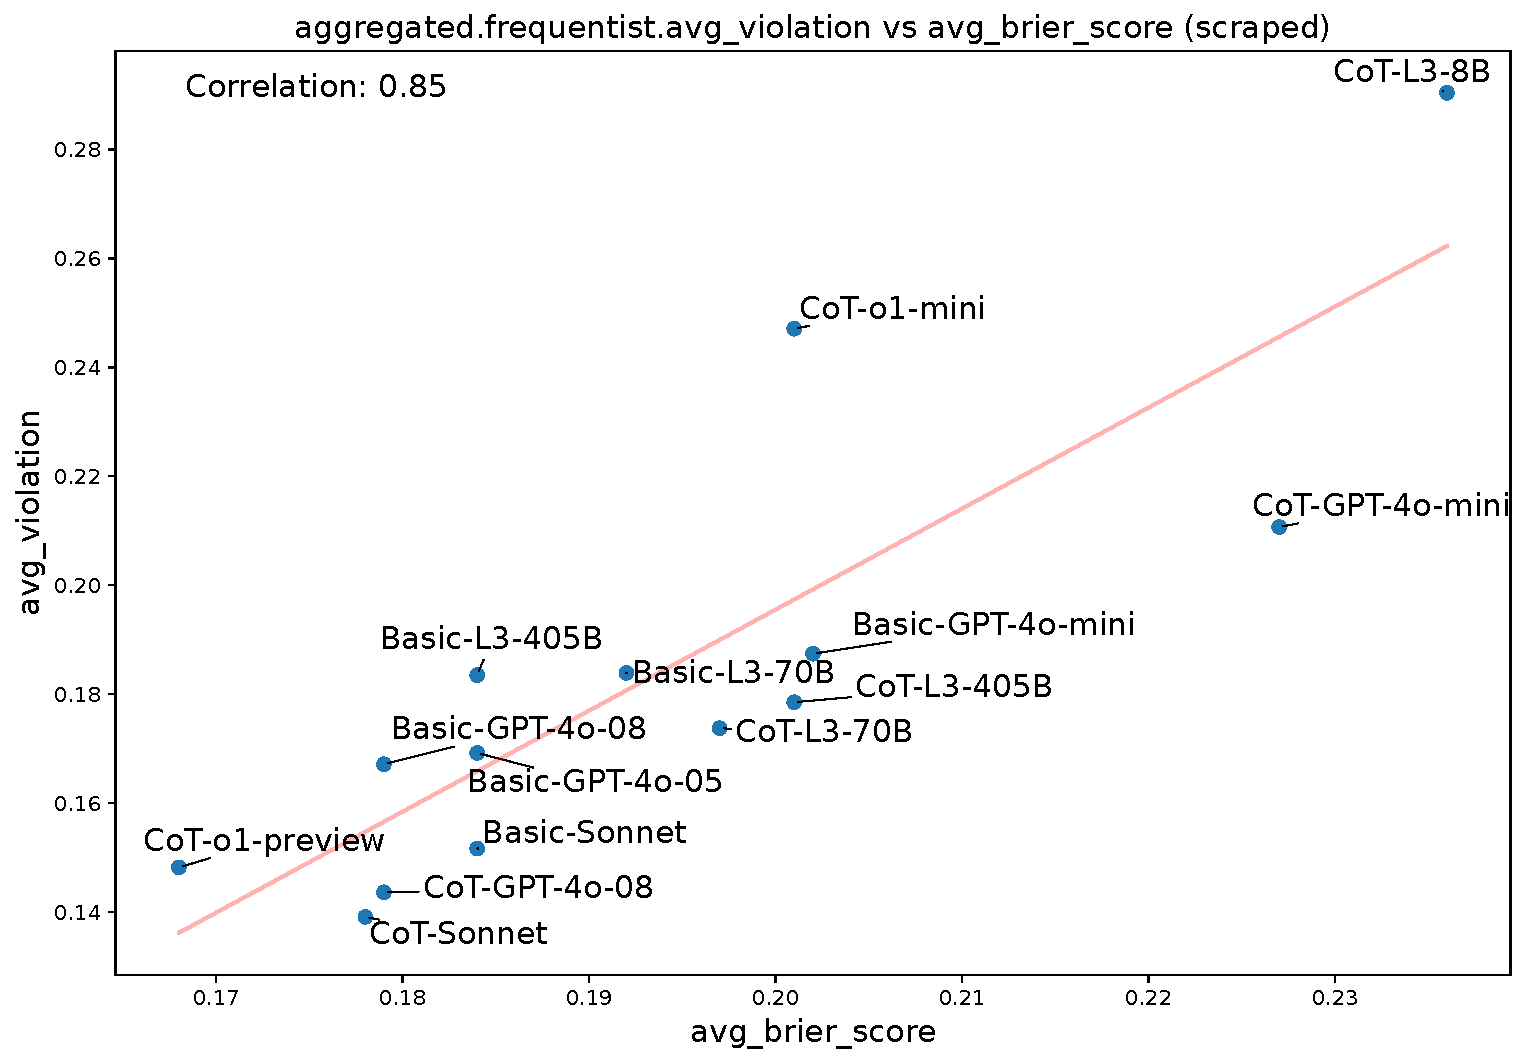
\includegraphics[width=\textwidth]{figures/consistency/aggregated_vs_avg_brier_score_frequentist_avg_violation_scraped.pdf}
        \caption{
         Aggregate frequentist metric on the scraped forecasting question dataset.
        }
        \label{fig:aggregate_vs_avg_brier_frequentist_scraped}
    \end{subfigure}
    \hfill
    \begin{subfigure}[b]{0.48\textwidth}
        \centering
        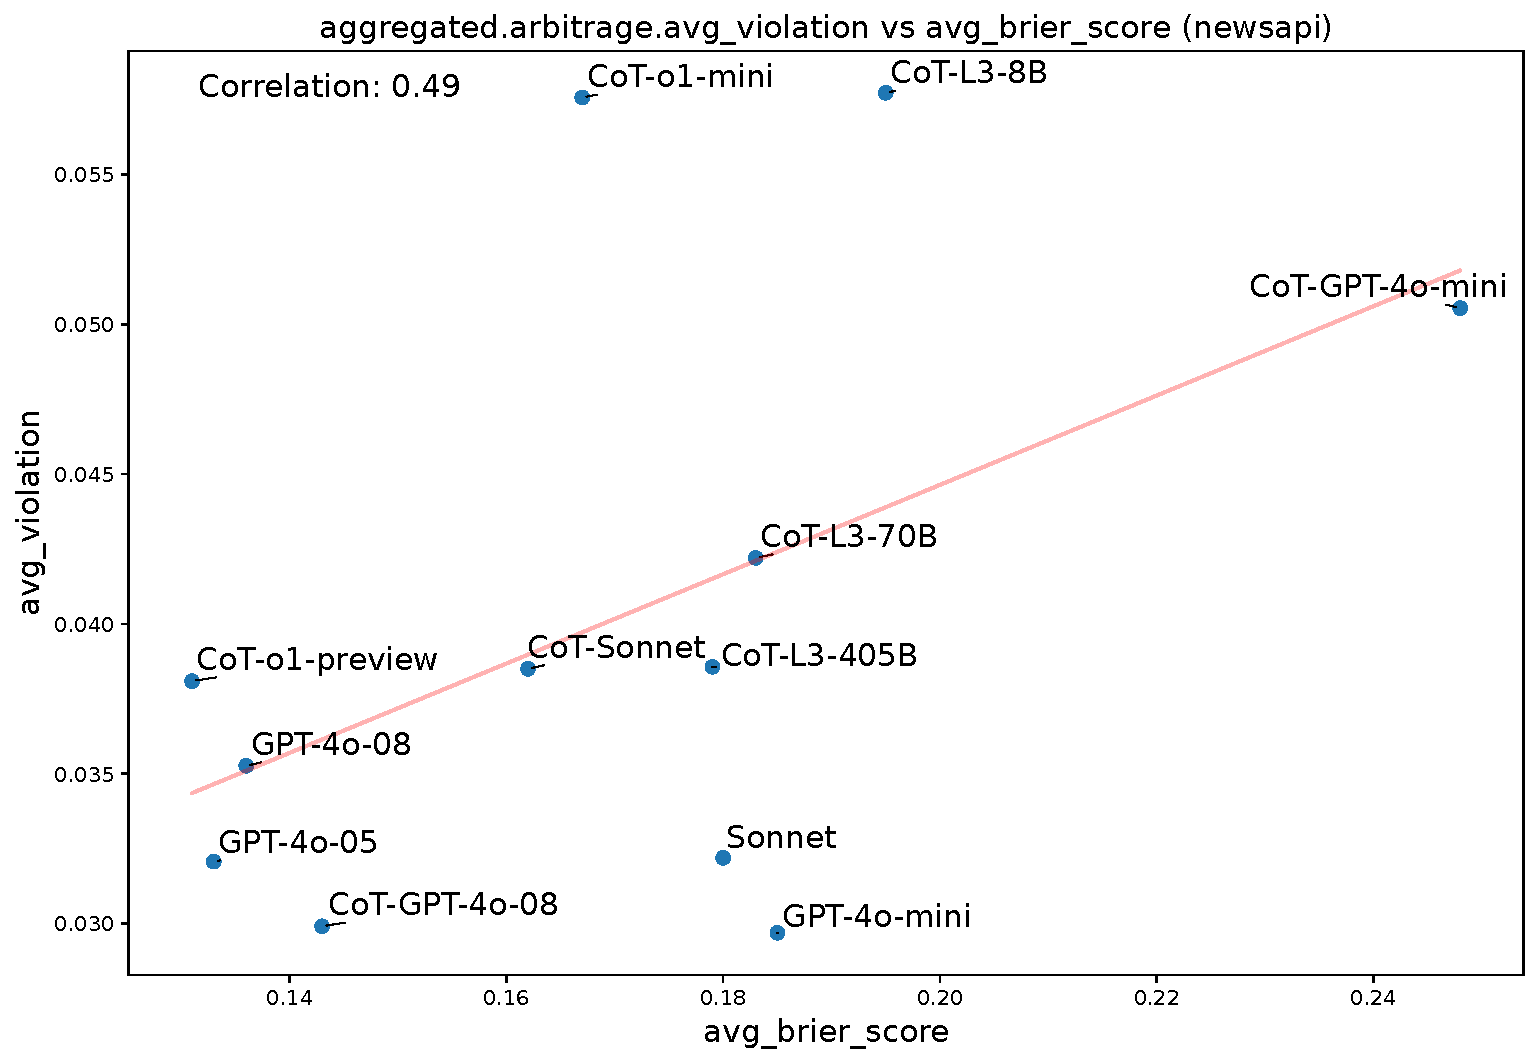
\includegraphics[width=\textwidth]{figures/consistency/aggregated_vs_avg_brier_score_default_avg_violation_newsapi.pdf}
        \caption{
         Aggregate arbitrage metric on the NewsAPI questions dataset.
        }
        \label{fig:aggregate_vs_avg_brier_arbitrage_newsapi}
    \end{subfigure}
    \caption{
        Scatter plots showing the relationship between consistency metrics and average Brier scores for different forecasters.
        Each point represents a forecaster, with the x-axis showing the average Brier score and the y-axis showing the consistency metric .
        The y-axis values are aggregated across all checks for each forecaster and averaged over the instantiated consistency check tuples.
        Lower scores are better for both axes.
    }
    \label{fig:consistency_vs_brier}
\end{figure}


\begin{figure}[h]
    \centering
    \begin{subfigure}[b]{0.48\textwidth}
        \centering
        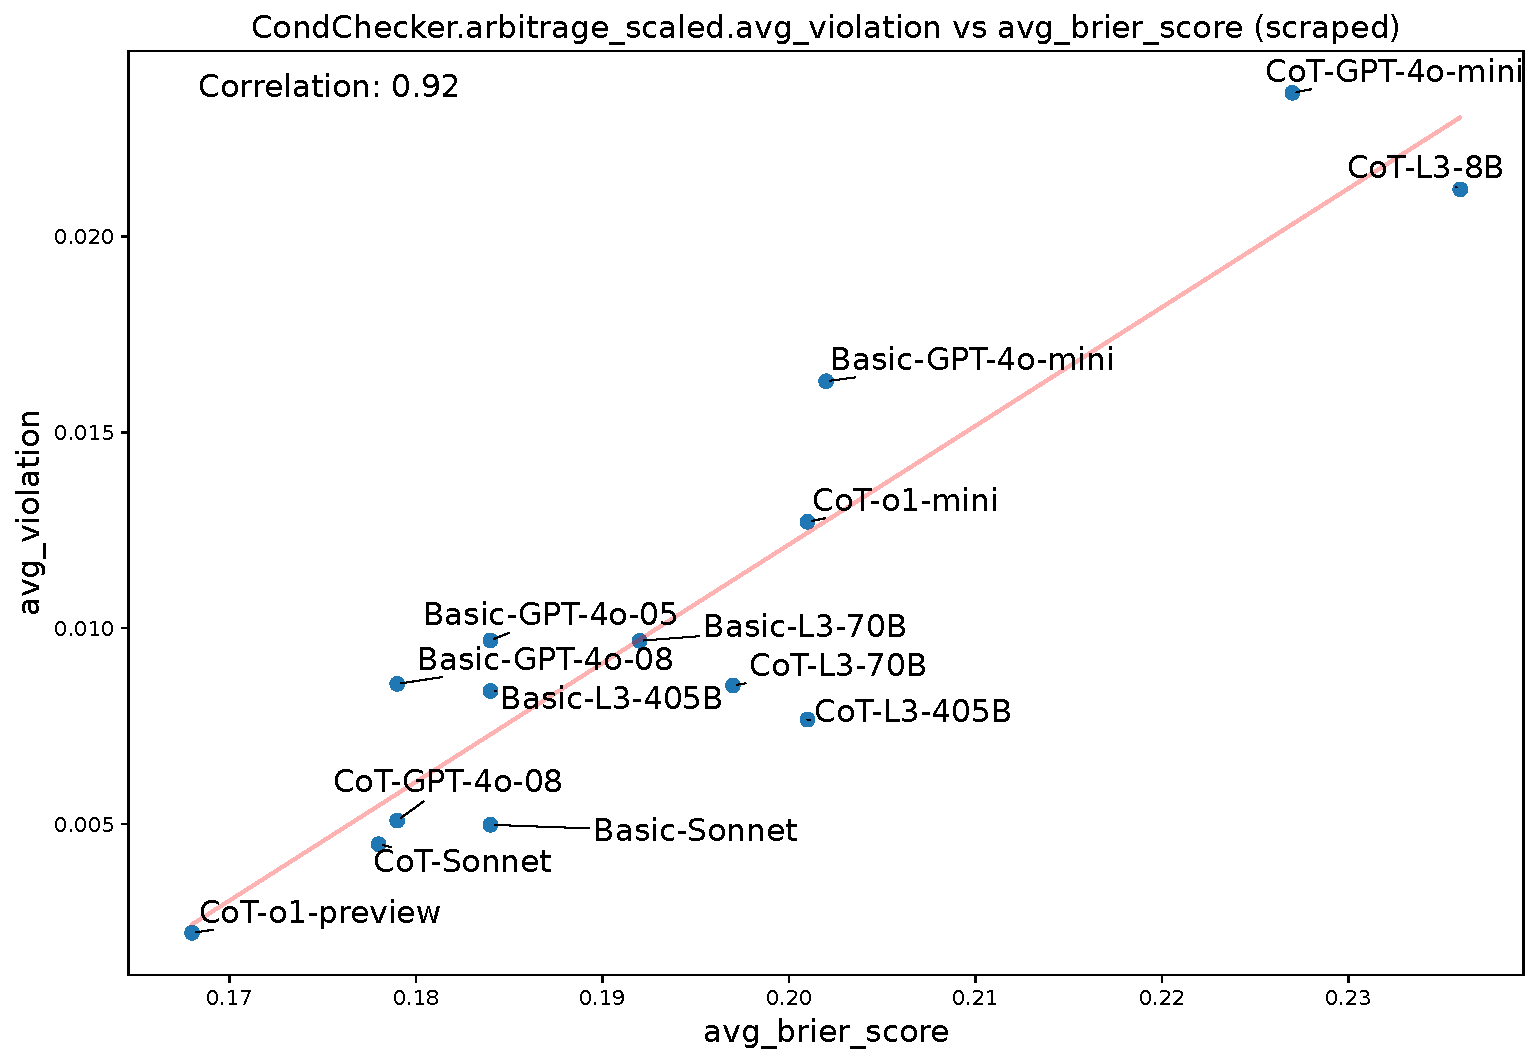
\includegraphics[width=\textwidth]{figures/consistency/CondChecker_vs_avg_brier_score_default_scaled_avg_violation_scraped.pdf}
        \caption{
         \CondChecker{} arbitrage metric on the scraped forecasting question dataset.
        }
        \label{fig:condchecker_vs_brier_scraped}
    \end{subfigure}
    \hfill
    \begin{subfigure}[b]{0.48\textwidth}
        \centering
        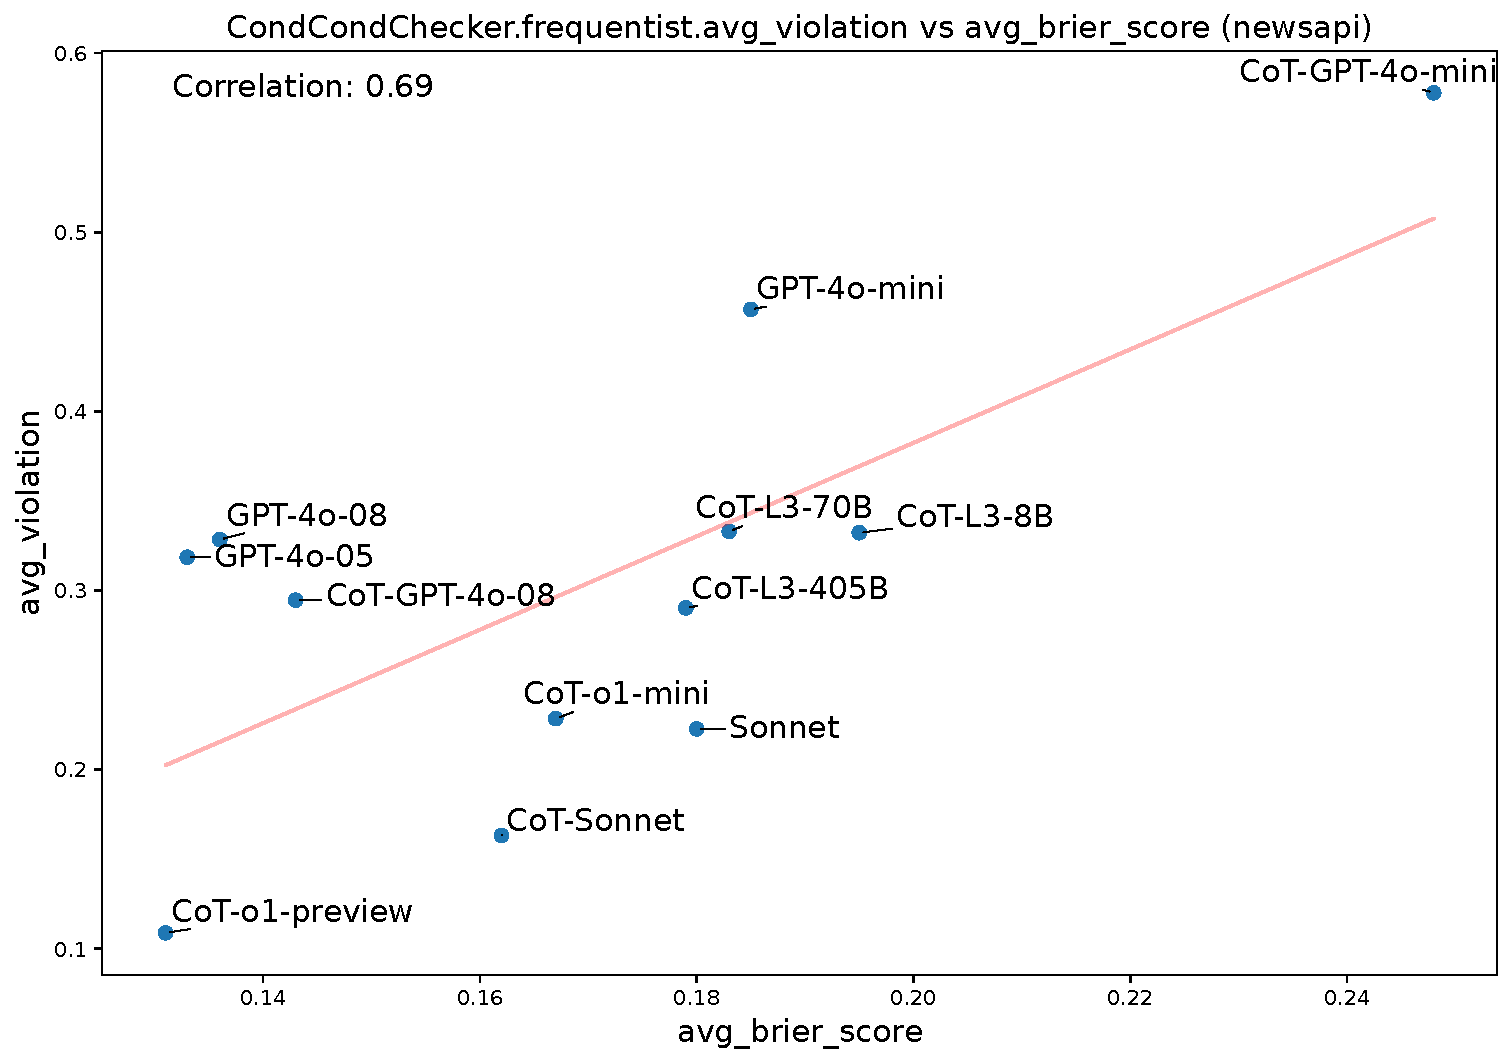
\includegraphics[width=\textwidth]{figures/consistency/CondCondChecker_vs_avg_brier_score_frequentist_avg_violation_newsapi.pdf}
        \caption{
        \CondCondChecker{} frequentist metric on the NewsAPI questions dataset.
        }
        \label{fig:condcondchecker_vs_brier_newsapi}
    \end{subfigure}
    \caption{
        Both \CondChecker{} and \CondCondChecker{} consistency metrics \rebuttal{see \Cref{tab:consistency_checks}} show a strong correlation with forecasting accuracy as measured by the Brier score.
    }
    \label{fig:consistency_vs_brier-condchecker}
\end{figure}


\textbf{Bayesian consistency checks are the best proxies for forecasting performance.}
Figure \ref{fig:condchecker_vs_brier_scraped} shows the strong correlation between certain consistency checks
\rebuttal{from \Cref{tab:consistency_checks}}
and average Brier scores across different forecasters.
This relationship suggests that \CondChecker{}, which tracks logical consistency in conditional probability estimates, serves as \rebuttal{a proxy} for overall forecasting accuracy, \emph{without knowing how the questions resolved}.


\textbf{Certain consistency metrics are not well correlated with forecasting performance.}
The measured correlations between the consistency checks and Brier scores are given in \Cref{tab:consistency-correlations}. We see that some checks yield higher signal on the ground truth performance than others.
Aggregating different consistency metrics seems to improve the correlation.

We note that the selection of forecasters we test is quite limited,
%(see \Cref{cfc/sec:cannot_evaluate_halawi})
so we cannot guarantee the trends here are representative of future LLM forecasters.
%trends here need to be taken with a grain of salt. \vin{refine - trends here should be taken as purely demonstrative.}
\rebuttal{Part of the correlation can be attributed to better models being both more consistent and better forecasters. For comparison, the correlations of the Brier score of our forecasters and the MMLU \cite{mmlu} (college split) error rate on the best approximation of the tested forecasters are 0.38 and 0.55 on the NewsAPI and scraped datasets, respectively.}

We include all data (questions, tuples, forecasts, and scores) in the supplementary material.

\begin{table*}[hbp]
    \centering
   \caption{Correlation of consistency metrics with Brier score, across both of our base question datasets and the derived consistency check tuples.}
   \label{tab:consistency-correlations}
   \small
   \begin{tabular}{lrrrr}
     \toprule
     & \multicolumn{2}{c}{Scraped} & \multicolumn{2}{c}{NewsAPI} \\
     \cmidrule(lr){2-3} \cmidrule(lr){4-5}
     & Arbitrage & Frequentist & Arbitrage & Frequentist \\
     \midrule
     \NegChecker{} & 0.60 & 0.67 & -0.36 & -0.13 \\
     \ParaphraseChecker{} & 0.57 & 0.61 & 0.13 & 0.24 \\
     \ConsequenceChecker{} & 0.51 & 0.52 & 0.21 & 0.30 \\
     \AndOrChecker{} & 0.20 & 0.25 & 0.02 & 0.06 \\
     \AndChecker{} & 0.68 & 0.72 & 0.54 & 0.71 \\
     \OrChecker{} & 0.14 & 0.24 & -0.24 & -0.31 \\
     \ButChecker{} & 0.20 & 0.67 & 0.63 & 0.77 \\
     \CondChecker{} & 0.92 & 0.87 & 0.71 & 0.69 \\
     \CondCondChecker{} & 0.78 & 0.71 & 0.75 & 0.69 \\
     \ExpectedEvidenceChecker{} & 0.20 & 0.77 & -0.11 & 0.06 \\
     Aggregated & 0.62 & 0.85 & 0.49 & 0.66 \\
     \bottomrule
   \end{tabular}
   \label{tab:consistency-correlations-2}
 \end{table*}


\textbf{Even good reasoning models are inconsistent.}
We give the full set of consistency metrics for OpenAI's \oonemini{} in \Cref{tab:o1-mini}.
The \texttt{Frac} column counts the fraction of tuples for which the violation exceeded a certain threshold; see the full exposition of what the thresholds mean in \Cref{cfc/app:arbitrage,cfc/app:frequentist-metric}.
The frequentist metric is not directly comparable to the arbitrage metric, but the respective violation counts (``Frac'' in the table) are.

%\adamunimp{these 2 paragraphs should be cut or moved.  Why are we explaining the cutoffs for the arbitrage metric and frequentist metric here?}For the arbitrage metric, this threshold is $10^{-2}$, corresponding to the arbitrage profit between two forecasts of $0.5$ and $0.6$ on \NegChecker{}.
%For the frequentist metric, this is determined by rejecting the null hypothesis of a Monte Carlo forecaster, at significance level $p<0.01$.
%The full exposition of the frequentist metric is in \Cref{cfc/app:frequentist-metric}.
%The violation threshold for the frequentist metric is chosen to be at the metric value of the $(0.5,0.6)$ pair for \NegChecker{}.


\begin{table*}[htbp]
\centering
  \caption{Consistency metrics for o1-mini.}
  \label{tab:o1-mini}
  \small
  \begin{tabular}{@{} lrrrrrrrr @{}}
    \toprule
    & \multicolumn{4}{c}{Scraped} & \multicolumn{4}{c}{NewsAPI} \\
    \cmidrule(lr){2-5} \cmidrule(lr){6-9}
    & \multicolumn{2}{c}{Arbitrage} & \multicolumn{2}{c}{Frequentist} & \multicolumn{2}{c}{Arbitrage} & \multicolumn{2}{c}{Frequentist} \\
    \cmidrule(lr){2-3} \cmidrule(lr){4-5} \cmidrule(lr){6-7} \cmidrule(lr){8-9}
    Check & Avg & Frac & Avg & Frac & Avg & Frac & Avg & Frac \\
    \midrule
    \NegChecker{} & $0.07$ & $58\%$ & $0.26$ & $61\%$ & $0.08$ & $52\%$ & $0.27$ & $56\%$ \\
    \ParaphraseChecker{} & $0.07$ & $56\%$ & $0.26$ & $61\%$ & $0.06$ & $53\%$ & $0.24$ & $56\%$ \\
    \ConsequenceChecker{} & $0.03$ & $27\%$ & $0.13$ & $29\%$ & $0.03$ & $18\%$ & $0.10$ & $19\%$ \\
    \AndOrChecker{} & $0.09$ & $65\%$ & $0.34$ & $71\%$ & $0.07$ & $57\%$ & $0.29$ & $67\%$ \\
    \AndChecker{} & $0.02$ & $24\%$ & $0.11$ & $27\%$ & $0.03$ & $23\%$ & $0.11$ & $24\%$ \\
    \OrChecker{} & $0.11$ & $48\%$ & $0.30$ & $50\%$ & $0.05$ & $48\%$ & $0.21$ & $50\%$ \\
    \ButChecker{} & $0.11$ & $60\%$ & $0.40$ & $79\%$ & $0.11$ & $63\%$ & $0.38$ & $80\%$ \\
    \CondChecker{} & $0.04$ & $41\%$ & $0.22$ & $52\%$ & $0.07$ & $66\%$ & $0.29$ & $70\%$ \\
    \CondCondChecker{} & $0.03$ & $30\%$ & $0.19$ & $45\%$ & $0.04$ & $54\%$ & $0.23$ & $71\%$ \\
    \ExpectedEvidenceChecker{} & $0.04$ & $47\%$ & $0.27$ & $69\%$ & $0.05$ & $45\%$ & $0.28$ & $63\%$ \\
    \midrule
    \textbf{Aggregated} & $0.06$ & $-$ & $0.25$ & $-$ & $0.06$ & $-$ & $0.24$ & $-$ \\
    \bottomrule
  \end{tabular}
\end{table*}
OpenAI's \oonemini{} forecaster, despite being one of the best reasoning models so far, violates consistency checks more than the $(0.5, 0.6)$ threshold from \Cref{cfc/sec:forecasting} very often.

% \textbf{Long-horizon consistency benchmark.}
% The results of the previous section indicate that, even on longer time horizons where it's not possible to have ground truth resolutions, we can still evaluate and compare different forecasters via consistency metrics.

% We create a dataset of 900 synthetic questions resolving in 2028 and create 3000 tuples in total from this dataset using the method described in \Cref{cfc/sec:instantiation}, to evaluate the consistency of the forecasters in questions with a longer horizon, where it's not
% possible to have the ground truth resolutions. Examples of questions and the results for \gptfouro{} are in \Cref{cfc/app:synthetic-questions-2028}.

% We intend this dataset as a working prototype for a continual long-term forecasting benchmark.
%\adamunimp{This section is kinda week.  Like who cares, you have a bunch of questions that willnot resolve in the near future.  If keep, at least mention how it can be useful as a continual benchmark for future studies}

\section{\CFCaster{}: Can we design a more consistent forecaster?}
\label{cfc/sec:cfcaster}

\rebuttal{Let $(x_1,\dots x_n)$ be a question tuple for some consistency check $\Relation$, e.g. $(P,\lnot P)$. Given forecasts $\Forecaster(x_1), ... \Forecaster(x_n)$, the arbitrage metric maximization problem in ~Equation ~\ref{eq:arbitrage__} computes the following (as the argmax and max of the arbitrage respectively):}

\begin{enumerate}
    \item Improved forecasts $\Forecaster'(x_1), ... \Forecaster'(x_n)$ which are consistent, i.e. satisfy $\CCheck$; and
    \item The profit earned by an arbitrageur who bets these improved forecasts against the original ones -- this is the actual metric.
\end{enumerate}

This leads us to wonder: \emph{can we use these ``improved consistent forecasts'' to build a new forecaster which builds on the base forecaster $\Forecaster$, but is more consistent on $\Relation$}?

We introduce: the \CFCaster{} with base $\Forecaster$ arbitraged on consistency check $\Relation$, denoted by $\CFC[\Relation]{\Forecaster}$, which computes its forecast on a question $x$ as follows:
\begin{enumerate}
    \item Instantiates a tuple $(x_1,\dots x_n)$ satisfying $\Relation$;
    \item Queries $\Forecaster$ to obtain $\Forecaster(x_1),\dots\Forecaster(x_n)$;
    \item Arbitrages these base forecasts per Eq~\ref{eq:arbitrage__} and returns the arbitraged forecast for $x_1$.
\end{enumerate}

\rebuttal{Despite what one might assume, however, an \CFCaster{} is \emph{not} ``definitionally'' consistent on the check it is arbitraged on, but rather its consistency must be investigated empirically. Suppose, for example, that a forecaster produces forecasts $\Forecaster(P)=0.5$, $\Forecaster(\operatorname{para}(P))=0.6$, $\Forecaster(\operatorname{para}(\operatorname{para}(P)))=0.7$. Then $\Forecaster':=\CFC[\ParaphraseChecker{}]{\Forecaster}$ would produce forecasts $\Forecaster'(P)\approx0.55$, $\Forecaster'(\operatorname{para}(P))\approx0.65$, which are not consistent.}

Appendix~\ref{cfc/app:cfcaster} contains a precise definition of \CFCaster{}, including the case of sequentially arbitraging on multiple checks $\CFC[[\Relation_1,\dots\Relation_s]]{\Forecaster}$, and a theoretical discussion of its consistency properties. In particular, we list strong theoretical reasons to expect consistency gains from \emph{recursive} \CFCaster{} setups, i.e. $\CFC[\Relation]{\Forecaster}^r:=\CFC[\Relation]{\CFC[\Relation]{\Forecaster}^{r-1}}$, in particular with \NegChecker{}, as well as in a non-recursive \CFCaster{} with \ExpectedEvidenceChecker{}.

Due to these priorities and the high costs of running recursive \CFCaster{}s (see Appendix~\ref{cfc/app:cfcaster-cost}), we limited ourselves to studying only a small number of \CFCaster{} setups, with a limited number of checks rather than the whole list; specifically: $\CFC[N]{g}^r$, $\CFC[P]{g}^r$, $\CFC[[N,P]]{g}^r$, $\CFC[[E]*s]{g}$ where $g:=$\gptfouromini{}, $N,P,E$ are \NegChecker{}, \ParaphraseChecker{}, \ExpectedEvidenceChecker{} respectively, and $r$ and $s$ vary from 0 to 4.

% A single call to $\CFC[\vec{C}]{\Forecaster}$ involves $1+\sum_i (n_{\Relation_i}-1)$ calls to $\Forecaster$, plus several LLM calls for each $\FullInstantiator_i$ depending on the exact instantiation process (see Appendix~\ref{cfc/app:cfcaster-cost} for details) -- running this for all checks in Table~\ref{tab:consistency_checks} can get quite expensive, especially for the recursive \CFCaster{}s we are interested in. Thus in our experiments we limited ourselves to studying only a small number of \CFCaster{} setups, with a limited number of checks, specifically we experimented with: $\CFC[N]{g}^r$, $\CFC[P]{g}^r$, $\CFC[[N,P]]{g}^r$, $\CFC[[E]*r]{g}$ where $g:=$\gptfouromini{}, $N,P,E$ are \NegChecker{}, \ParaphraseChecker{}, \ExpectedEvidenceChecker{} respectively, and $r$ varies from 0 to 4.
% \begin{itemize}
%     \item $\CFC[\NegChecker{}]{\gptfouromini{}}^r$ (denoted in tables and plots as CF-Nr)
%     \item $\CFC[\ParaphraseChecker{}]{\gptfouromini{}}^r$ (denoted in tables and plots as CF-Pr)
%     \item $\CFC[[\NegChecker{},\ParaphraseChecker{}]]{\gptfouromini{}}^r$ (denoted in tables and plots as CF-NPr)
%     \item $\CFC[[\ExpectedEvidenceChecker{}]*r]{\gptfouromini{}}$ (denoted in tables and plots as CF-rxEE1)
% \end{itemize}

The full results of our experiments with these forecasters are reported in Appendix~\ref{cfc/app:cf-results}; our key takeaways from these preliminary runs look hopeful:

\begin{itemize}
    \item In the case of the checks we tested, \textbf{arbitraging on a check indeed makes a forecaster more consistent on that check}\vin{change to emph rather than textbf}, with increasing consistency gains with recursive depth, as shown in Fig~\ref{fig:cf-4}. Crucially, this also applied when the arbitraging was on more than a single check: $\CFC[[N,P]]{g}^r$ did well on \emph{both} \NegChecker{} and \ParaphraseChecker{}; arbitraging on the next check did not increase inconsistency on the first. We are cautiously optimistic that this may extend to the full list of checks in Table~\ref{tab:consistency_checks}.
   % once cost does not deter from testing it.
    %\manyu{not sure if this list sounds like too much inference based on too little}
    %\adamunimp{But it also made all of the other ones worse. should that be mentioned?}
    %\dpaleka{It made some of the other ones better and some worse}
    \item \textbf{This consistency gain was greatest with \NegChecker{}, followed by \ParaphraseChecker{}, and lowest with \ExpectedEvidenceChecker{}.} This finding is in line with our hypothesis in Appendix~\ref{cfc/app:cfcaster} that \CFCaster{} would be particularly effective on consistency checks which are \emph{symmetric}. and instantiate \emph{deterministically}.
    %\adamunimp{not sure how much this line adds}
    \item \textbf{We do not observe reliable improvements on ground truth forecasting performance, or on consistency checks other than the ones we arbitrage on.}
%    \adamunimp{again it actually does worse...My guess is that in trying to fix one parameter, it ignores the constraints of the others}
%    \dpaleka{it's not always worse, e.g. for \CondChecker{} it increases twice and decreases twice}
    I.e. $\CFC[\Relation_1]{\Forecaster}$ does not reliably do better on $\Relation_2$.
\end{itemize}

\begin{figure}[h]
    \centering
    \begin{subfigure}[b]{0.46\textwidth}
        \centering
        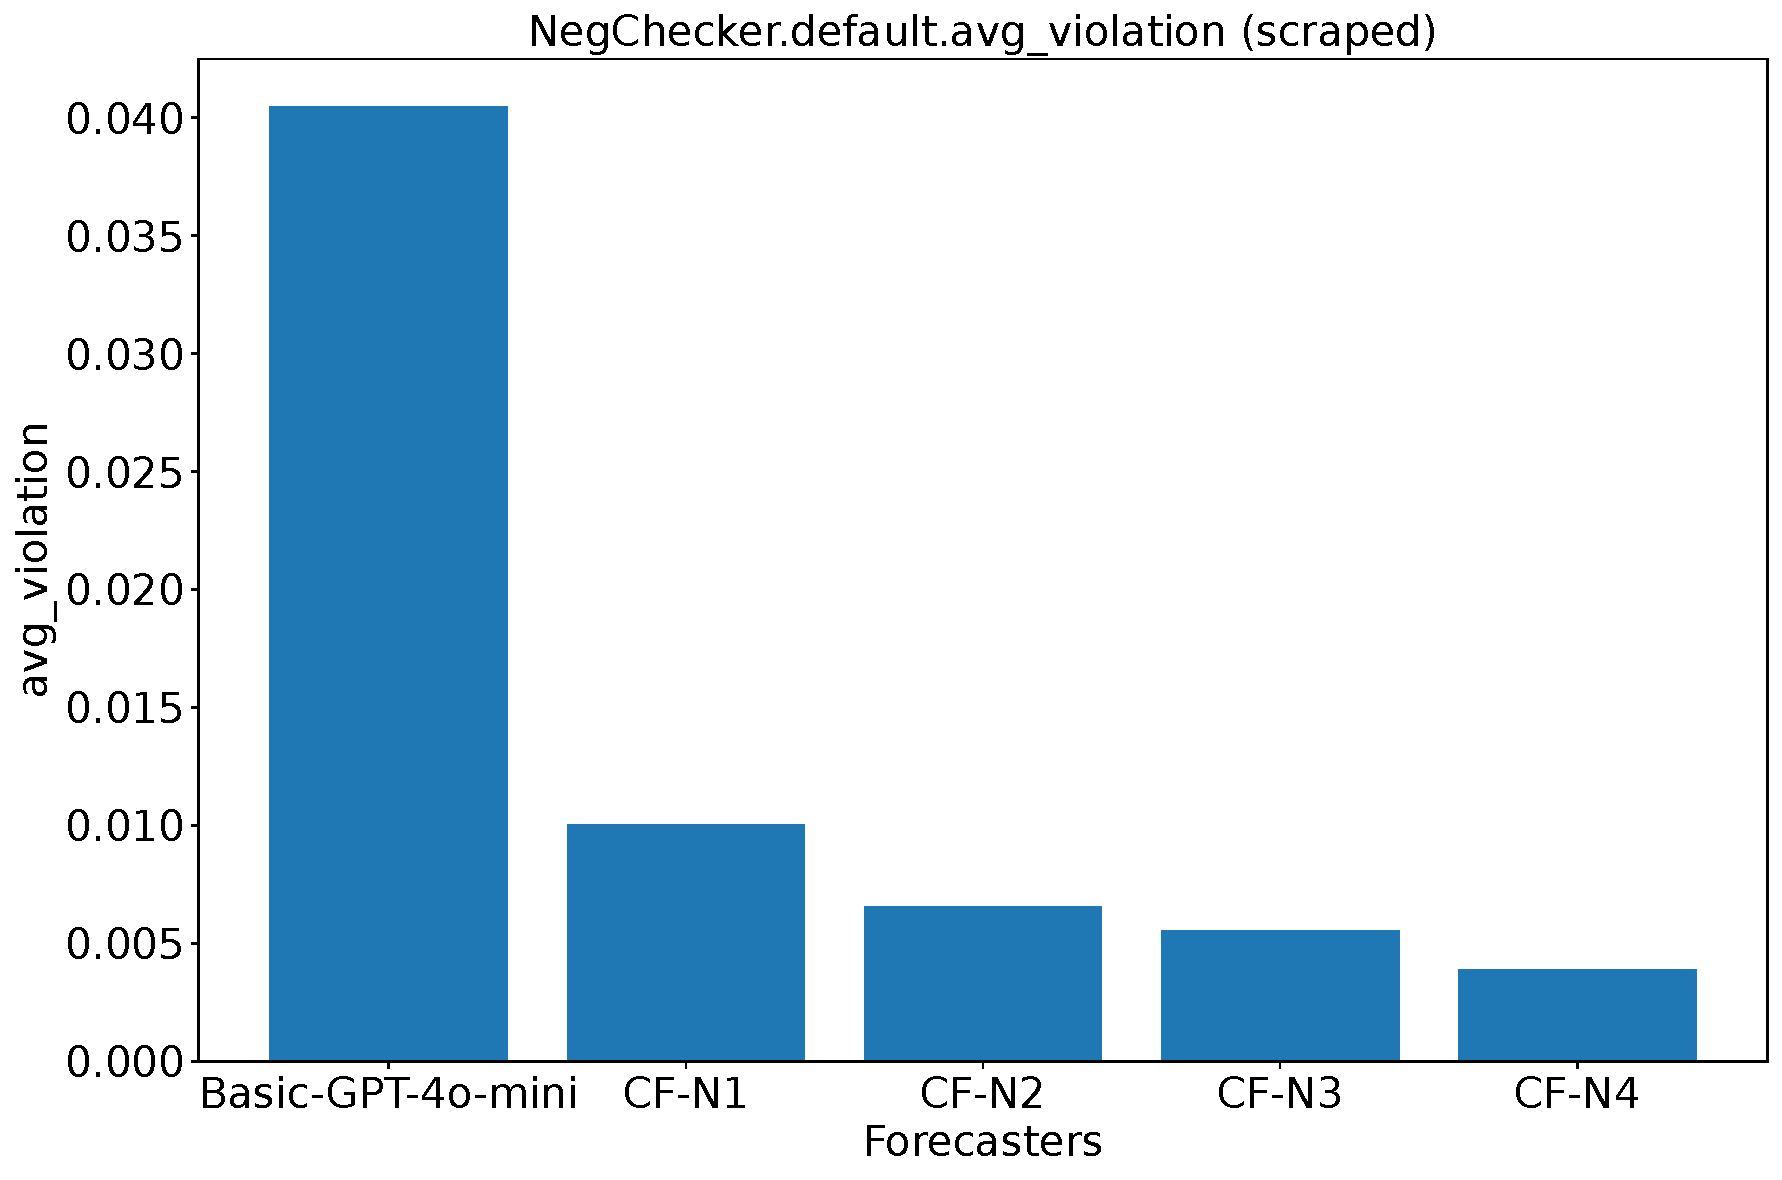
\includegraphics[width=\textwidth]{figures/consistency/cfcaster_scraped/N-N.pdf}
        \caption{Average violation of $\CFC[N]{g}^r$ (denoted CF-Nr) on \NegChecker{} for $r$ from 0 to 4.
        }
        \label{fig:N-N}
    \end{subfigure}
    \hfill
    \begin{subfigure}[b]{0.48\textwidth}
        \centering
        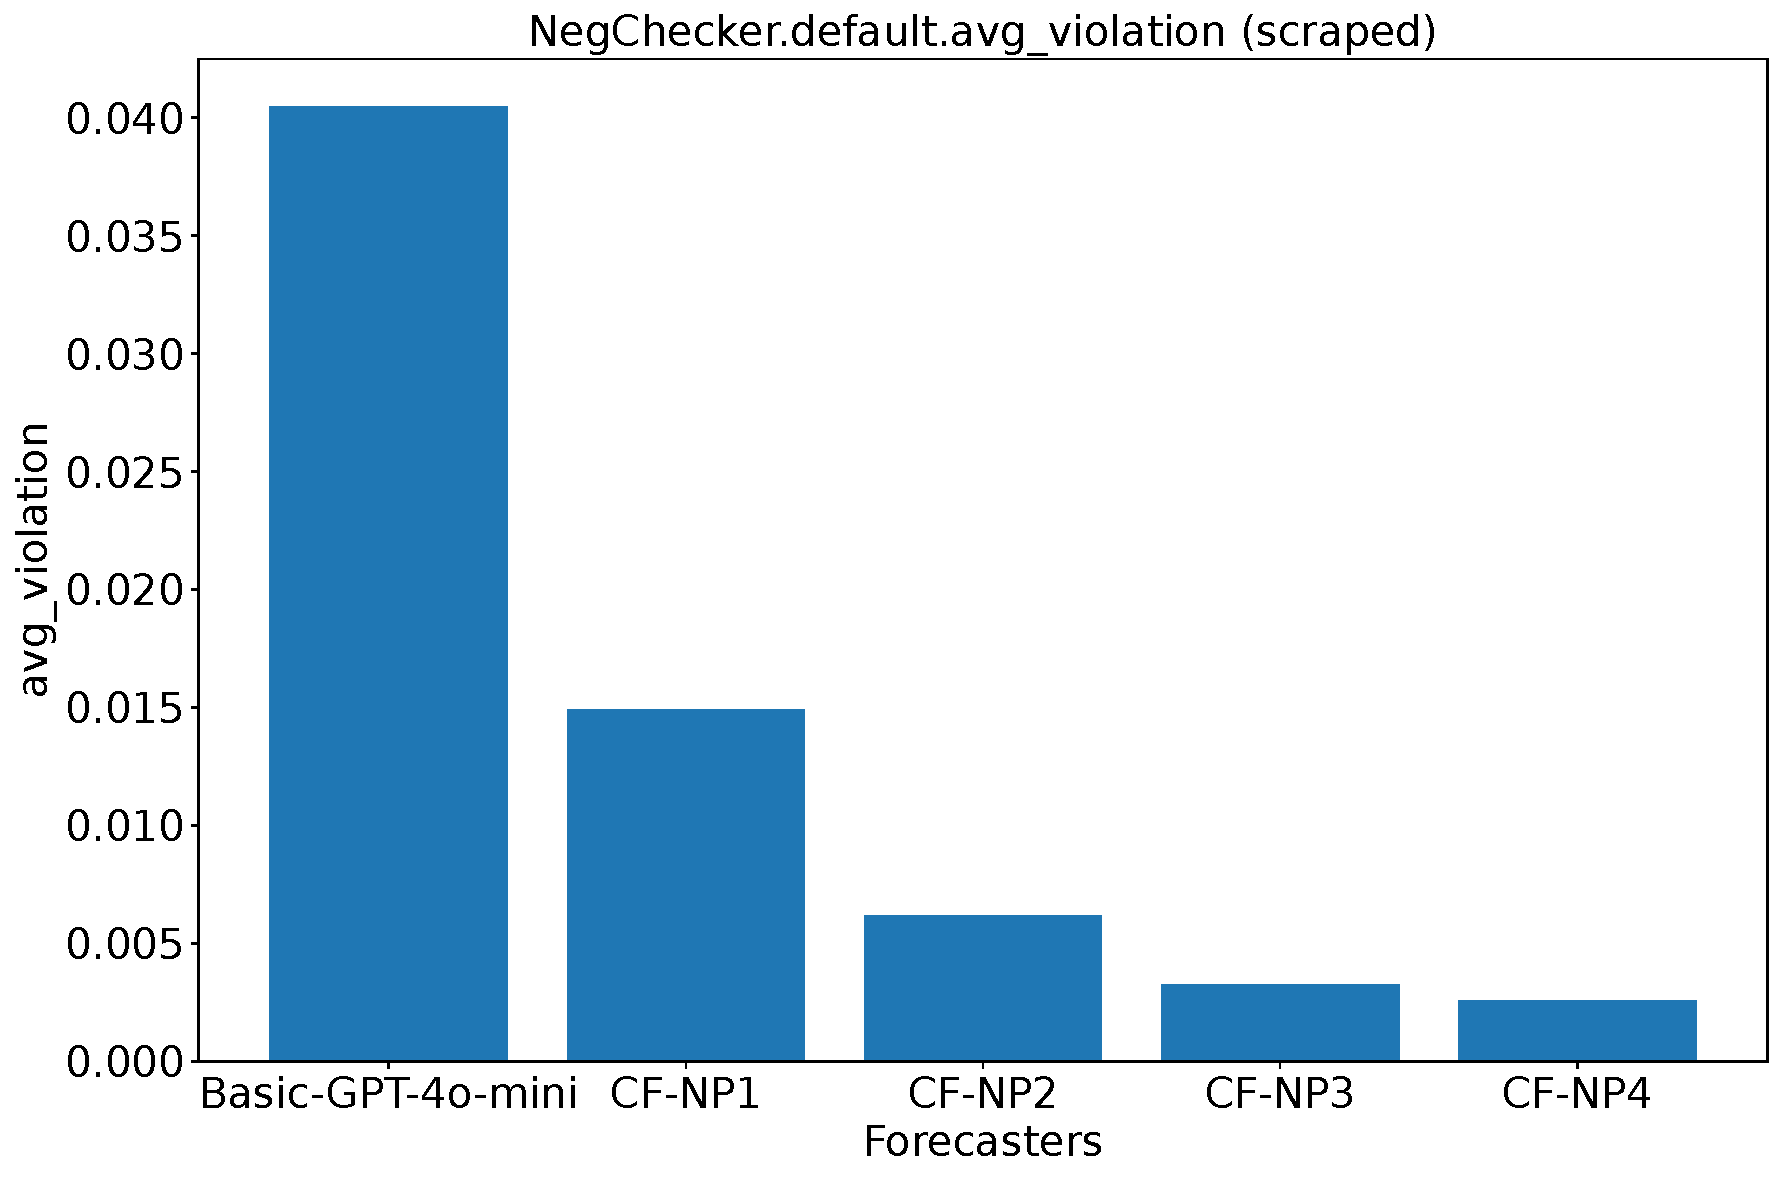
\includegraphics[width=\textwidth]{figures/consistency/cfcaster_scraped/NP-N.pdf}
        \caption{Average violation of $\CFC[NP]{g}^r$ (denoted CF-NPr) on \NegChecker{} for $r$ from 0 to 4.
        }
        \label{fig:NP-N}
    \end{subfigure}
    \begin{subfigure}[b]{0.48\textwidth}
        \centering
        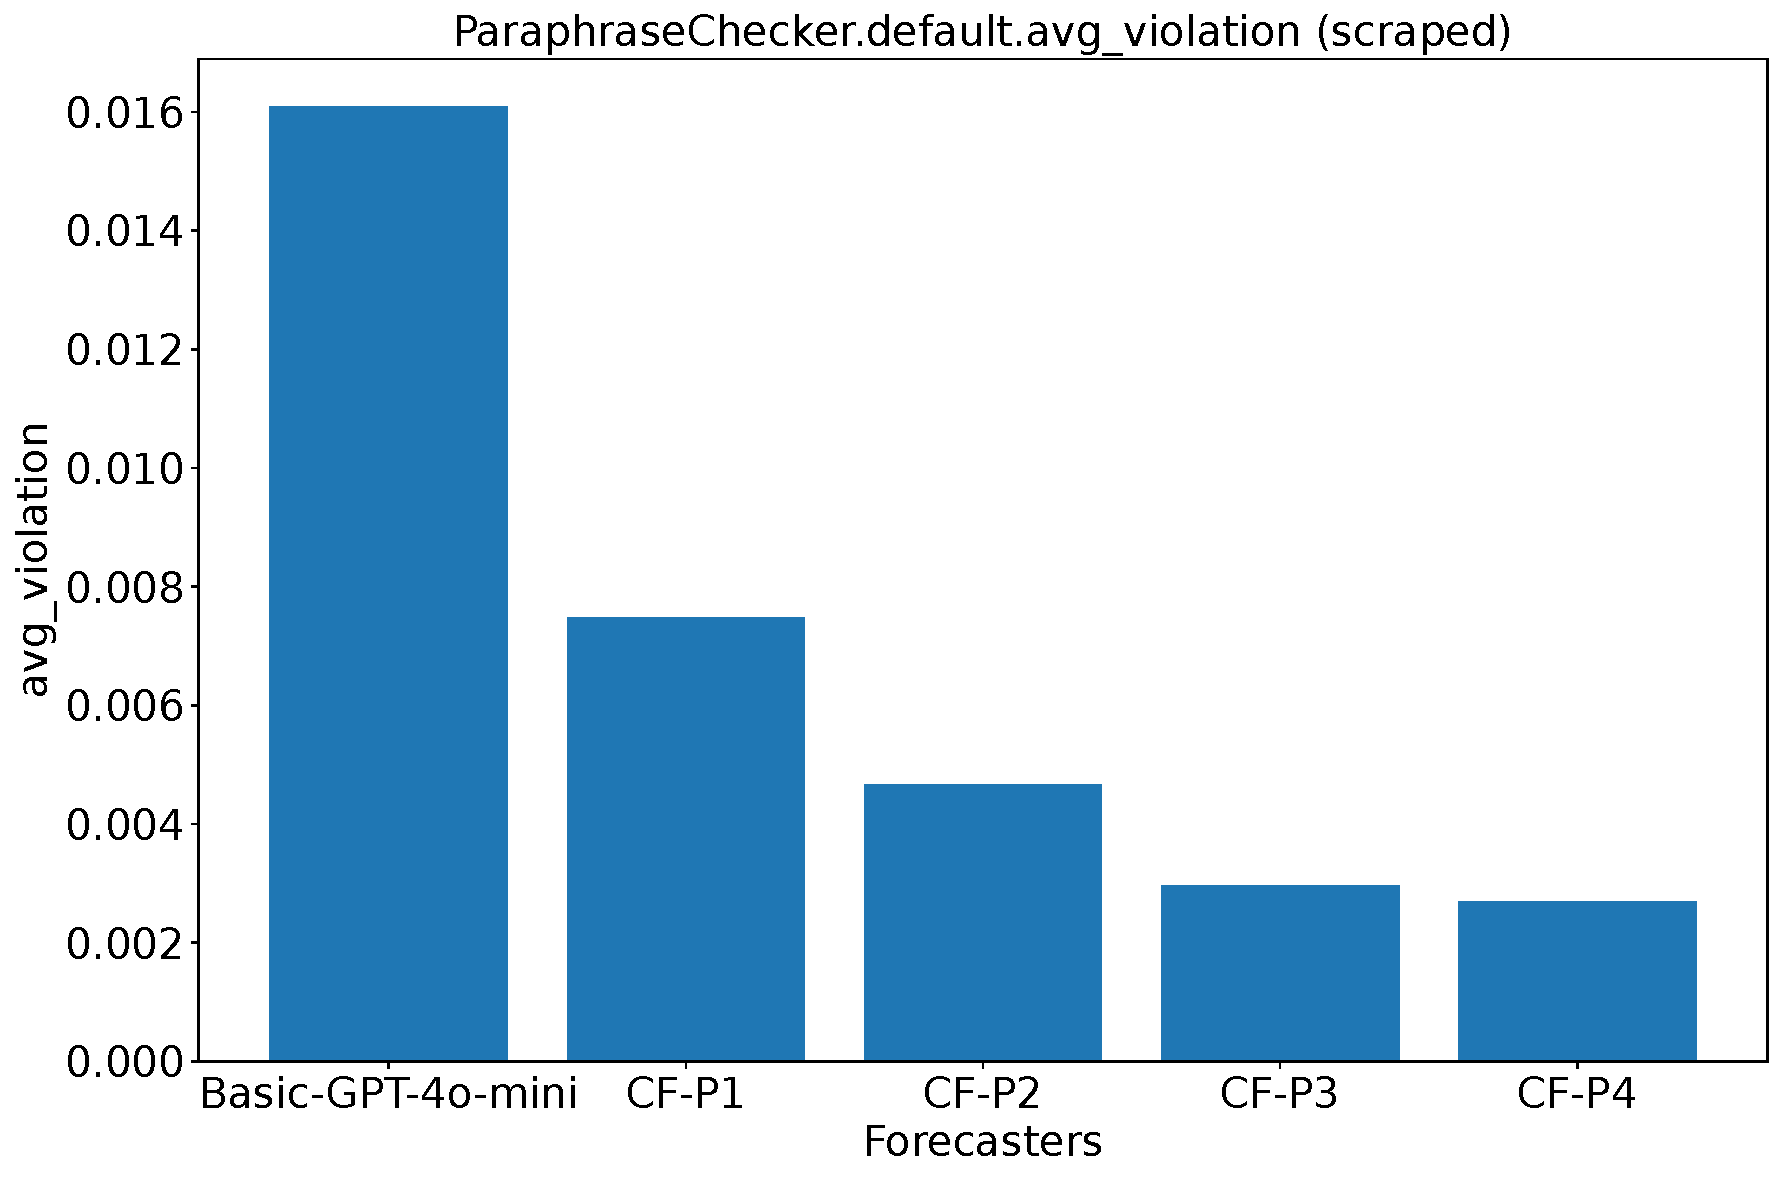
\includegraphics[width=\textwidth]{figures/consistency/cfcaster_scraped/P-P.pdf}
        \caption{
         Average violation of $\CFC[P]{g}^r$ (denoted CF-Pr) on \ParaphraseChecker{} for $r$ from 0 to 4.}
        \label{fig:P-P}
    \end{subfigure}
    \hfill
    \begin{subfigure}[b]{0.48\textwidth}
        \centering
        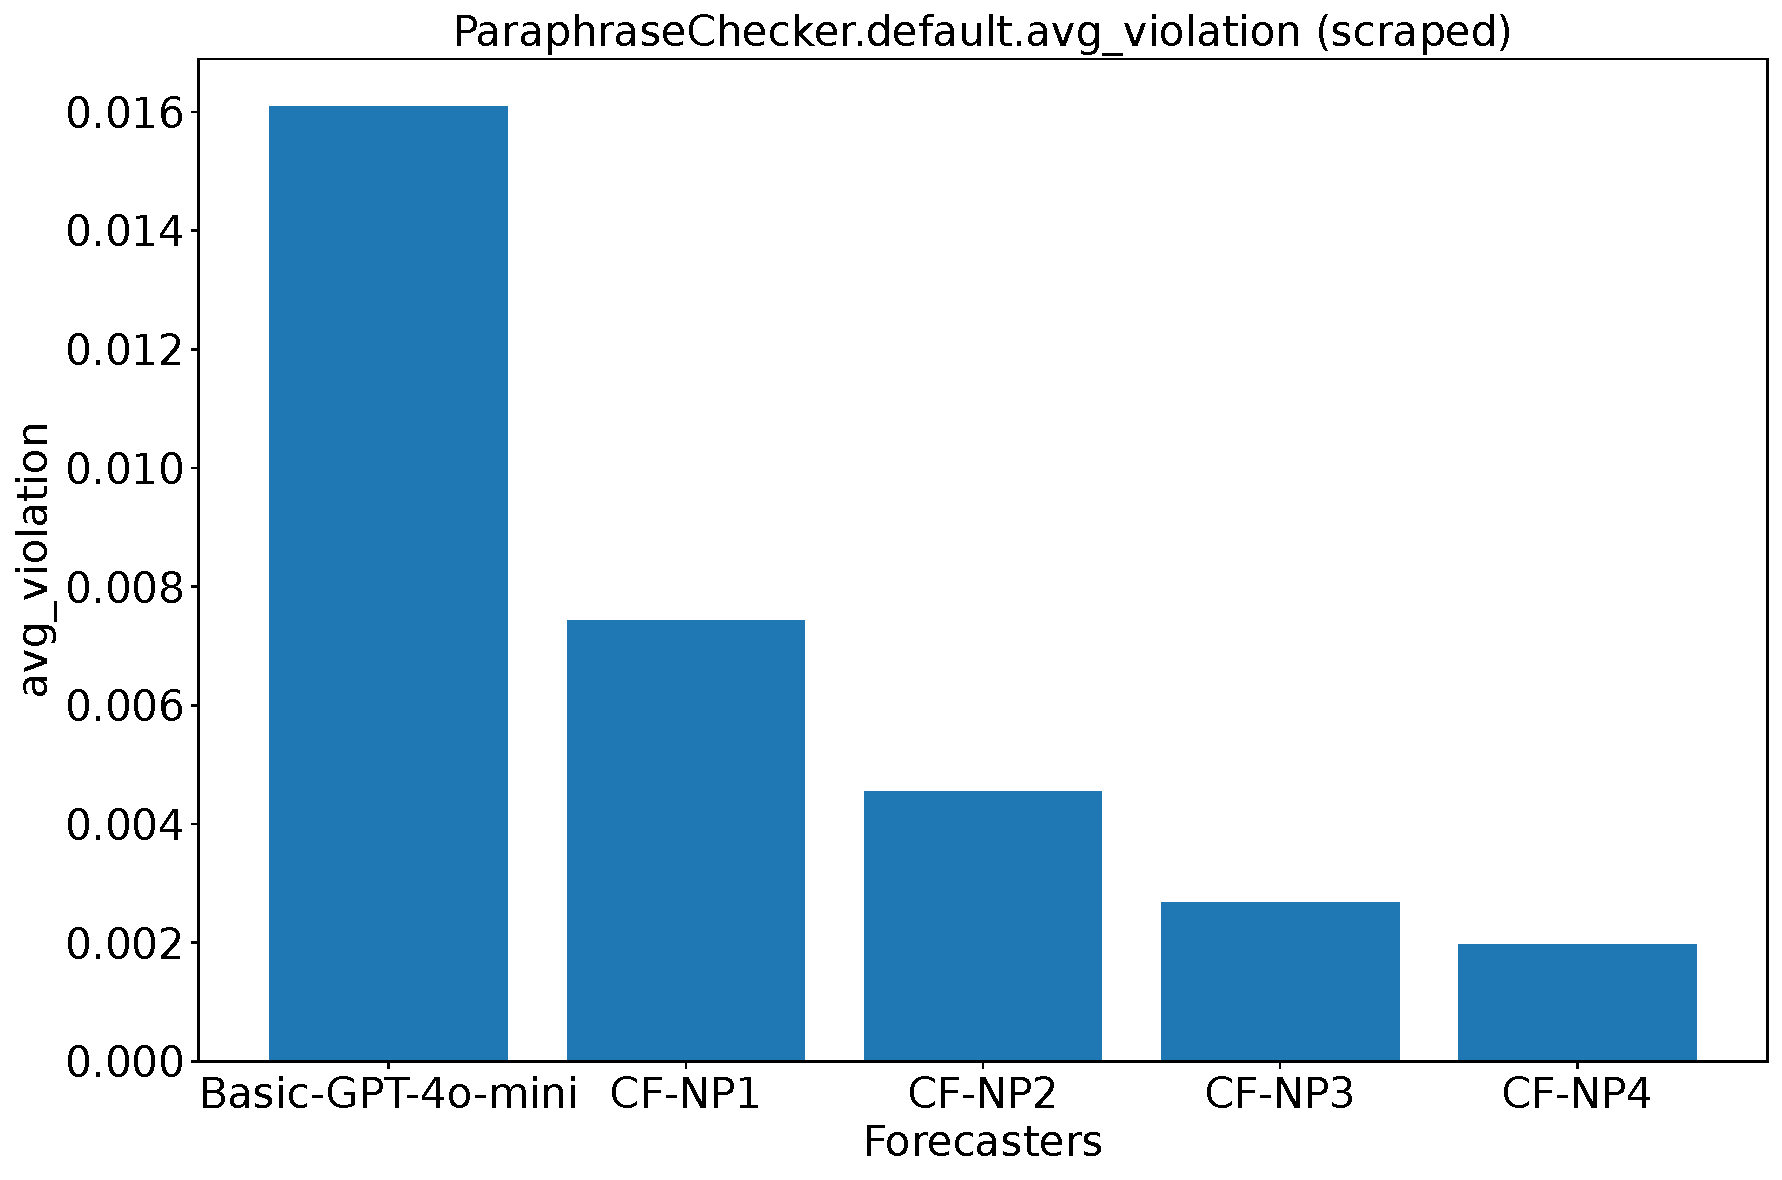
\includegraphics[width=\textwidth]{figures/consistency/cfcaster_scraped/NP-P.pdf}
        \caption{
         Average violation of $\CFC[NP]{g}^r$ (denoted CF-NPr) on \ParaphraseChecker{} for $r$ from 0 to 4.}
        \label{fig:NP-P}
    \end{subfigure}
    \caption{\NegChecker{} and \ParaphraseChecker{} violations for various \CFCaster{} setups. In all captions, $g$ denotes \gptfouromini{}, $N,P$ denote \NegChecker{} and \ParaphraseChecker{} respectively, and the definition of the \CFCaster{} setup is as in Def~\ref{def:cf}.}
    \label{fig:cf-4}
\end{figure}


\section{Related work}
\textbf{Metamorphic and consistency checks.}
Checking logical properties of outputs of programs under semantic-preserving transforms has a long history \citep{chen1998metamorphic}. Before \citet{esmwcc}, variants of the consistency check framework were used for simple ML models \citep{christakis2022specifying, sharma2020monotonicity}, vision \citep{hendrycks2019benchmarking}, and chat LLMs \citep{jang2023consistency}, among other areas.
\rebuttal{
\citet{li2019logic} consider logical consistency checks beyond paraphrasing and negation for simple ML models.
}
%Evaluating without ground truth in a fashion similar to this a long history as \emph{metamorphic testing} ...
%\todo{@dpaleka finish}

\textbf{Forecasting and large language models.}
LLMs and forecasting date back to \citet{zou2022forecasting} and \citet{yan2023autocast++}. Recently, strong performance of LLM forecasters on prediction market datasets has been claimed in \rebuttal{\citep{halawiApproachingHumanLevelForecasting2024, tetlock2024longrange, hsieh2024reasoning, safeai2024forecasters}}.
\rebuttal{
Concurrent with our work, \citet{karger2024forecastbench} have introduced an automatically updating benchmark for forecasting.
}

\textbf{Scalable oversight and failures of superhuman AI.}
The difficulty of evaluating models with superhuman performance in domains without a source of ground truth has long been acknowledged, and falls under the umbrella of \emph{scalable oversight}  \citep{amodei2016concrete}.
Forecasting using AI oracles is one such domain.  The use of consistency checks for scalable oversight has been studied in the simpler context of superhuman game AIs \citep{alphazero_not_robust, esmwcc},
and in general question-answering tasks via debate \citep{irving2018debate}.

\textbf{Consistency evaluations for LLMs.}
Even on tasks where the ground truth is in principle knowable,
consistency evaluations have long helped in cases where checking consistency is easier than getting the ground truth labels \citep{elazarPararel2021, liGeneratorValidatorConsistency2023}.
\rebuttal{
\citet{raj2023semantic} measure paraphrasing consistency and ground truth accuracy on TruthfulQA \citep{lin2021truthfulqa} and find little to no  correlation.
}
Some forms of consistency checks have been applied on model internals to discover features related to LLM truthfulness and reliability \citep{burnsDiscoveringLatentKnowledge2022, kaarelSearchingModelsConcepts2023}.


%{Failure modes in superhuman models.}
%ML models achieve undisputed superhuman performance for various games, e.g., chess~\cite{campbell2002deep, alphazero} or Go~\cite{alphago}.
%%\footnote{ML models also surpass human baselines on some benchmarks for vision, speech or natural language processing, but we do not consider these models as superhuman here, as the ground truth for these tasks is still defined from human knowledge.}
%Yet, game-playing agents for Go can be defeated by simple adversarial strategies designed against them~\cite{alphazero_not_robust, go_adversarial, go_adversarial2}.
%These strategies are either found ``end-to-end'' (via self-play against the victim)~\cite{go_adversarial, go_adversarial2},
%or by checking consistency over boards that appear semantically equivalent to an examiner (either a human observer or a stronger model)~\cite{alphazero_not_robust}.
%In contrast, we consider the problem of eliciting bugs in model decisions when a proxy for ground truth (better than the model being evaluated) is not available.
%{Scalable oversight.} Our work relates to the problem of \emph{scalable oversight}~\cite{amodei2016concrete},
%the ability to supervise models when  ground truth is hard or impossible to obtain (e.g., because model abilities match or exceed humans).
%Our work is complementary to prior methods, which make capable models and humans interact to extract confidently correct answers~\cite{bowman2022measuring, irving2018debate};
%we instead study how humans could probe such models for confidently \emph{incorrect} answers, i.e., human-verifiable bugs.
%
%{Model truthfulness.}
%There are many attempts at evaluating the truthfulness of language model outputs~\cite{evans2021truthful, lin2021truthfulqa}.
%%Our consistency checks can be viewed as a way of demonstrating model falsehoods in the absence of known ground truth.
%We envision that consistency tests could serve as a method for detecting when models provide dishonest answers or lies~
%\cite{burtell2023artificial, cicero-diplomacy, pan2023rewards, burns2022discovering, christiano2022elk},
%under the assumption that it is easier to provide consistent answers when telling the truth~\cite{irving2018debate}.

%\citet{liGeneratorValidatorConsistency2023} check consistency of LLMs are  \emph{generators} (``Write a sentence funnier than sentence X'') and \emph{validators} (``Is sentence X or Y funnier?'').
%This paradigm is applicable for a general AI system forecasting: we can use ``Give me an event which is more likely to happen than event X'' as a generator, and check the probabilities afterward.


\section{Future work}
\label{cfc/sec:future-work}
%\dpaleka{This section can be very short if needed}

We have developed a comprehensive benchmark of \emph{static consistency checks} for LLM forecasters, and demonstrated its correlation with ground truth accuracy, suggesting that our consistency metrics could serve as a proxy for accuracy when we do not have access to ground truth. We envision several directions in which our framework could be extended:

% summary

%\todo{rephrase probably, and maybe add some speculative idea that uses CCS}
%We foresee several promising directions:

\textbf{Consistency in decision-making.} AI systems may be used not only to make forecasts that inform decisions, but also to take decisions directly. Here too, we can have a notion of inconsistency: for example, \emph{intransitive preferences}
\footnote{See e.g. \cite{fishburnUtilityTheoryDecision1970} and the Von Neumann–Morgenstern utility theorem for an introduction to decision rationality.} -- and analogously, an inconsistent decision-maker may be exploited by an arbitrageur.

%We can think of an AI decision-maker as giving utility estimates to different options (and choosing the highest one), much like an AI forecaster gives probability estimates to different outcomes. However, the analogy is not completely straightforward, as AI decision makers may also differ on which options they list in their analysis. %A similarly thorough benchmark for decisional consistency will require some nontrivial insights on such considerations.

\textbf{Training for consistency.~}
Modulo consideration of the cost-benefit to safety,
our methods could be used train LLMs for consistency,
minimizing our violation metrics.
This may or may not impact overall forecasting performance and other AI capabilities.
%as well as measure if this improves truthfulness overall, e.g. by comparing answers to the model's internal beliefs.
One may also imagine an AlphaZero-style set-up, where an LLM $\Forecaster$ is trained on the outputs of $\CFC{\Forecaster}^r$, i.e. a recursive \CFCaster{} wrapped around it.

\rebuttal{\textbf{Further experiments with \CFCaster{}.} Most of our experiments with \CFCaster{} involved arbitraging on only a \emph{single} check (apart from one experiment with both \NegChecker{} and \ParaphraseChecker{}), due to the cost limitations described in \ref{cfc/app:cfcaster-cost}. It is easy to imagine how a bad forecaster could still overfit a single check: simply forecasting $50\%$ probability for all questions will pass \ParaphraseChecker{}, \ExpectedEvidenceChecker{} and  \NegChecker{} -- but we expect that being consistent under a variety of checks is difficult without a consistent world model. One approach to using more checks cheaply, particularly in training, may be to \emph{randomly sample} a number of consistency checks for each question.}

\textbf{Dynamic generation of consistency checks.~}
Although we found strong correlations between ground truth accuracy and consistency among existing LLM forecasters, our results with \CFCaster{} demonstrate that this isn't necessarily the case: it is possible to do well on consistency without improving ground truth. In particular, this means that consistency as a training metric could be ``Goodharted'' by a learning AI model \citep{karwowskiGoodhartsLawReinforcement2023}. One way to prevent this may be via adversarial training: i.e. have an adversarial agent instantiate consistency checks that it believes the agent will perform poorly on.

%via Contrast-Consistent Search \cite{burnsDiscoveringLatentKnowledge2022a}.
%\todo{does this make sense? @dpaleka}

%\textbf{Performative prediction.} what if the world model is nontrivially influenced by the forecaster's answer \todo{dpaleka this was your idea; you should explain it}
%

\textbf{Evaluating RAG-augmented forecasters.~}
\label{cfc/sec:cannot_evaluate_halawi}
We have conducted some preliminary experiments evaluating state-of-the-art forecasters such as \cite{halawiApproachingHumanLevelForecasting2024}.
% [we acknowledge the help of Danny Halawi in adapting this]
Unfortunately, we could not reproduce the system from \cite{halawiApproachingHumanLevelForecasting2024} at the time of writing, due to deprecations in the Google News API (we could not obtain access to the alternative Newscatcher API).
At the time of writing, we are not aware of other publicly-available LLM forecasting systems that are competitive with the results of \cite{halawiApproachingHumanLevelForecasting2024}
(there exist proprietary systems that may be competitive, such as \cite{futuresearch2024}).
We thus leave the evaluation of better forecasters like \cite{halawiApproachingHumanLevelForecasting2024} and \cite{safeai2024forecasters} to future work, once such forecasters are more widely available.
%The main contribution of this work is a benchmark, not developing a new forecasting system.



%\begin{enumerate}
%    \item Ground truth forecasting results:
%    \begin{itemize}
%        \item Contains a JSONL file where each entry specifies:
%        \begin{itemize}
%            \item The question with a boolean \texttt{resolution} field
%            \item The forecasted probability and forecast metadata like chain of though traces
%            \item The obtained Brier score and other metrics
%        \end{itemize}
%        \item The total Brier score can be obtained by averaging individual scores.
%    \end{itemize}
%
%    \item Consistency checks results:
%    \begin{itemize}
%        \item Contains a JSONL and a JSON file for each consistency check:
%        \begin{enumerate}
%            \item Raw results file, where each entry is a tuple of questions with the forecast for each question, along with forecast metadata like chain of thought traces;
%            \item Summary statistics file, which statistics like average violation.
%        \end{enumerate}
%    \end{itemize}
%\end{enumerate}


\section*{Contributions}
\label{cfc/app:contributions}

DP and APS developed consistency checks and the arbitrage and frequentist metrics.
DP, AA, APS, and EW worked on the LLM question to evaluation pipeline.
APS thought of and implemented \CFCaster{}.
VB created the news-derived question dataset.
AS and DP created the scraped question dataset.
AA and DP created the 2028 synthetic question dataset.
DP started and led the project.
FT proposed correlating consistency with forecasting accuracy and advised the project.
All authors helped with the writing.
DP and APS wrote the first draft of the paper.

\section*{Acknowledgements}
We thank Danny Halawi for extensive discussions and help with our setup. We thank Brendan Murphy, Ezra Karger, Fred Zhang, and Tatsunori Hashimoto for helpful discussions and feedback on the paper and forecasting in general.
We thank Berkeley SPAR for connecting collaborators, and BERI for partially funding the project.

% \appendix

% \begin{appendix}
\section{Appendix}
\subsubsection{Table of consistency checks}
\label{cfc/app:checks}

Table~\ref{tab:full-consistency_checks} (extended version of Table~\ref{tab:consistency_checks}) includes all the consistency checks tested for in our benchmark. In most of them, we leave the logical relations between forecasting questions $\Relation$ implicit by constructing the sentences directly. For instance, $\Relation(x_1,x_2):=x_1=\lnot x_2$ is implied by simply writing $x_1, x_2$ as $P, \lnot P$. In the rest of the appendix, we use the sentence-based ($P, Q$ instead of $x_1, x_2$) notation. %\todo{is this extending beyond the margins?}

\begin{table*}[hbtp]
    \centering
    \caption{Consistency checks and the logical consistency conditions.}
    \vspace{5pt}
    \label{tab:full-consistency_checks}
    % \begin{tabular}{l p{3.7cm} p{7cm}}%{|l|p{6cm}|p{6cm}|}
    \begin{tabular}{l p{0.25\linewidth} p{0.4\linewidth}}
    \toprule
    \textbf{Name} &
    \textbf{Tuple} &
    \textbf{Condition ($\CCheck$)}
    %& \textbf{Violation Metric ($\Violation$)}
    \\ \midrule
    %\\ \hline
    \NegChecker &
    $(P,\lnot P)$ &
    $\Forecaster(P)+\Forecaster(\lnot P)=1$
    \\ \midrule
    \begin{tabular}{@{}l@{}} \ParaphraseChecker\\ $\Relation(P,Q):=P\iff Q$\end{tabular} &
    $(P,Q)$&
    $\Forecaster(P)=\Forecaster(Q)$
    \\ \midrule
    \begin{tabular}{@{}l@{}} \ConsequenceChecker\\ $\Relation(P,Q):=P\implies Q$\end{tabular} &
    $(P,Q)$&
    $\Forecaster(P)\le\Forecaster(Q)$
    \\ \midrule
    \AndOrChecker &
    $(P,Q,P\land Q,P\lor Q)$ &
    $\Forecaster(P)+\Forecaster(Q)=\Forecaster(P\lor Q)+\Forecaster(P\land Q)$
    \\ \midrule
    \AndChecker &
    $(P,Q,P\land Q)$ &
    $\max(\Forecaster(P)+\Forecaster(Q)-1, 0) \le \Forecaster(P\land Q) \le \min(\Forecaster(P),\Forecaster(Q))$
    \\ \midrule
    \OrChecker &
    $(P,Q,P\lor Q)$ &
    $\max(\Forecaster(P),\Forecaster(Q))\le\Forecaster(P\lor Q)\le\min(1,\Forecaster(P)+\Forecaster(Q))$
    \\ \midrule
    \ButChecker &
    $(P,\lnot P\land Q, P\lor Q)$ &
    $\Forecaster(P\lor Q)=\Forecaster(P)+\Forecaster(\lnot P\land Q)$ %
    \\ \midrule
    % \SymmetryAndChecker & $\Forecaster(P\land Q)=\Forecaster(Q\land P)$
    % \\ \midrule
    % \SymmetryOrChecker & $\Forecaster(P\lor Q)=\Forecaster(Q\lor P)$
    % \\ \midrule
    \CondChecker &
    $(P,Q|P,P\land Q)$ &
    $\Forecaster(P)\Forecaster(Q|P)=\Forecaster(P\land Q)$
    \\ \midrule
    %\CondCondChecker &
    %$(P,Q|P,R|(P\land Q),P\land Q\land R)$ &
    %$\Forecaster(P)\Forecaster(Q|P)\Forecaster(R|P\land Q) =\Forecaster(P\land Q\land R)$
    \CondCondChecker &
    \begin{tabular}[t]{@{}p{3.7cm}@{}}
    $(P,Q|P,R|(P\land Q),$\\
    $P\land Q\land R)$
    \end{tabular} &
    $\Forecaster(P)\Forecaster(Q|P)\Forecaster(R|P\land Q) =\Forecaster(P\land Q\land R)$
    \\ \midrule
    \ExpectedEvidenceChecker &
    $(P,Q,P|Q,P|\lnot Q)$&
    $\Forecaster(P)=\Forecaster(P|Q)\Forecaster(Q)+\Forecaster(P|\lnot Q)(1-\Forecaster(Q))$
    \\ \bottomrule
    \end{tabular}
\end{table*}

The consistency checks in Table~\ref{tab:full-consistency_checks} represent core logical relationships between probabilities, but many other forms of consistency checks are possible. Here are two examples that could extend our framework:

\begin{itemize}
    \item \textbf{Comparative checks:} Building on generator-validator checks from \citet{liGeneratorValidatorConsistency2023}, we could ask a forecaster to predict both $\Forecaster(P)$, $\Forecaster(Q)$, and separately whether $P$ or $Q$ is more likely. The forecaster's probability estimates should match their comparative judgment.

    \item \textbf{Monotonicity checks:} \citet{esmwcc} propose a variant of \ConsequenceChecker{} for real-valued quantities, where predictions must respect the monotonic ordering of a sequence of future values. \rebuttal{This connects to \emph{scope insensitivity} \citep{kahneman2000economic}, a cognitive bias where humans fail to scale probability estimates appropriately with the magnitude of outcomes.}
\end{itemize}

We do not include a specific consistency check for Bayesian updates, as conditional probabilities are already covered by \CondChecker{}, \CondCondChecker{}, and \ExpectedEvidenceChecker{}.

\subsubsection{Arbitrage as a violation metric}
\label{cfc/app:arbitrage}

\rebuttal{For the following definition we use a slightly more general notation than in the main body, to convey that our methods could be generalized beyond binary forecasting questions. }

\begin{notation*}

    \rebuttal{Let $\ForecastingQuestions$ denote the set of forecasting questions we are interested in, $\Resolutions$ denote the set of possible outcomes/resolutions for an individual question, and $\Forecasts$ denote the set of probability distributions on $\Resolutions$. A \emph{Forecaster} is a map $\Forecaster:\ForecastingQuestions\to\Forecasts$. For conditional questions that can resolve to $\none$, we also have optional resolutions $\ResolutionsOpt:=\Resolutions\cup\{\none\}=\boolsopt$.}
\end{notation*}


The arbitrage metric may be seen as being motivated by Dutch Book Arguments for probabilistic consistency rules (see e.g. \cite{vinebergDutchBookArguments2022}). Imagine the forecaster's predictions $\Forecaster(x_1),\dots\Forecaster(x_n)$ were prices offered by a bookie on prediction markets for sentences $x_1,\dots x_n$. If these probabilities are inconsistent, then there are bets that an arbitrageur can make that guarantee a profit in \emph{all possible (consistent) worlds regardless of the individual outcomes}. For example, if $x_1,x_2$ are two sentences such that $x_1\iff x_2$, but the bookie prices $\Forecaster(x_1)<\Forecaster(x_2)$, then an arbitrageur can simply buy $x_1$ and sell $x_2$ to make a risk-free profit.

However, if the bookie never changes their prices in response to trades, the arbitrageur can make an infinite amount of profit with its strategy. This is neither realistic nor useful for creating a metric to measure inconsistency. Instead, we turn to \emph{market scoring rules}, introduced in \citet{hansonLogarithmicMarketScoring2002}), where the bookie is a \emph{market-maker} who updates market prices in a way that ensures that the reward for moving the market price of a sentence that resolves True from $p_0$ to $p'$ is given by a \emph{proper scoring rule} \footnote{A proper scoring rule \citep{savageElicitationPersonalProbabilities1971}, is one that incentivizes honest reporting of probabilities: widely used proper scoring rules include the Brier score $(1-p)^2$ and the logarithmic scoring rule $-\log p$.} $s(p')-s(p_0)$. We then define our inconsistency metric to be the minimum profit an arbitrageur can guarantee against such a market-maker, if the latter offers inconsistent probabilities $\Forecaster(x_1),\dots\Forecaster(x_n)$.

\begin{definition}[Arbitrage-based Violation Metric]
    Let $\Relation:\ForecastingQuestions^n\to\bools$ be an n-ary relation such that $\Relation(\Resolution(x_1), \dots \Resolution(x_n))$ is satisfied by the ground-truth resolutions $\Resolution:\ForecastingQuestions\to\Resolutions$ for all tuples $(x_1,\dots x_n)$. \footnote{This is well-defined because resolutions can be taken as a subset $\Resolutions\subseteq\ForecastingQuestions$, by treating them as forecasting questions that always resolve to themselves by definition. For example, the forecasting question $\top$ is always worth \$1 and the forecasting question $\bot$ is always worth \$0.} Let $s:\ForecastingQuestions\times\Resolutions\times[0,1]\to\Reals$ be a proper scoring rule that gives the score earned based on the probability assigned to the true resolution, e.g. $s(x,\Resolution,p(\Resolution))=\log p(\Resolution)$. Let $(x_1,\dots x_n)\in\ForecastingQuestions^n$ be a question tuple, and denote $\ResolutionsVec:=\{\resolutionvec\in\ResolutionsOpt^n\mid\Relation(\resolutionvec)\}$ the set of possible consistent resolutions (including $\none$ resolutions) of this tuple. Then for forecasts $(\Forecaster(x_1),\dots\Forecaster(x_n))$ the arbitraged forecasts $\Arbitrageur(\Forecaster(x_1),\dots\Forecaster(x_n))=(p_1\dots p_n)$ and the minimum guaranteed profit of the arbitrageur $\Violation(\Forecaster(x_1),\dots\Forecaster(x_n))$ are given by:

    \begin{equation}
        \argmaxmax_{\consp\in\Forecasts^n}
        \min_{\resolutionvec\in\ResolutionsVec}
        \sum_{i=1}^n
        %\sum_{\Resolution\in\Resolutions}
        \score{x_i, \resolutionvec_i, p_i(\resolutionvec_i)}
        - \score{x_i, \resolutionvec_i, \Forecaster(x_i)(\resolutionvec_i)}%\Indicator{\omega_i=\Resolution}
        \label{eq:arbitrage}
    \end{equation}
    Where by convention, any score on a resolution $\resolutionvec_i=\none$ is taken to be 0.
    \label{def:arbitrage}
\end{definition}

Definition~\ref{def:arbitrage} is presented in full generality: $\consp$ and $\Forecaster(x_i)$ here are \emph{probability distributions} on $\Resolutions$. Breaking it down: each $\score{x_i, \resolutionvec_i, p_i(\resolutionvec_i)}- \score{x_i, \resolutionvec_i, \Forecaster(x_i)(\resolutionvec_i)}$ gives the arbitrageur's profit on the market for question $x_i$, given that it resolves $\resolutionvec_i$. The profit is summed across all markets in the tuple, and then minimized over all consistent worlds; this minimum is maximized across all possible arbitrageur bets.

It is helpful to explicitly state Eq~\ref{eq:arbitrage} in the case of binary forecasting questions, as follows.

\begin{equation}
    \argmaxmax_{\consp\in[0,1]^n} \min_{\omega\in\Omega} \sum_{i=1}^n \left(\score{\consp_i}-\score{\Forecaster(x_i)}\right)\Indicator{\omega(i)=\top} + \left(\score{1-\consp_i}-\score{1-\Forecaster(x_i)}\right)\Indicator{\omega(i)=\bot}
    \label{eq:arbitrage_}
\end{equation}



% \NewDocumentCommand{\score}{m}{\ensuremath{s\left(#1\right)}}
% \NewDocumentCommand{\consp}{}{p}
% \NewDocumentCommand{\argmaxmax}{}{\mathop{(\argmax,\max)}}

% If an arbitrageur could trade
% inconsistent probabilities offered on the market for arbitrary amounts of money, the profit would be infinite.
% This is neither realistic nor useful.
% In real-world markets (both prediction and financial),
% the mechanism that resolves this is
% a \emph{market maker}: an entity that accepts trades at market probabilities, but updates them slightly on every trade.

% A proper scoring rule, introduced in \cite{savageElicitationPersonalProbabilities1971}, is one that incentivizes honest reporting of probabilities.
% \citet{hansonLogarithmicMarketScoring2002} shows that the \emph{logarithmic scoring rule} has useful properties for modeling the market maker.

% \todo{Manyu: write here. or maybe it's better that Daniel writes this so he understands

% TODO explain how we get the log thing.
% }

% The arbitrage metric may be seen as being motivated by Dutch Book Arguments for probabilistic consistency rules (see e.g. \cite{vinebergDutchBookArguments2022}). The idea is as follows: imagine the forecaster's predictions $\Forecaster(P_1),\dots\Forecaster(P_n)$ were prices offered by a bookie on prediction markets for sentences $P_1,\dots P_n$. If these probabilities are inconsistent, then there are bets that an arbitrageur can make that guarantee a profit in \emph{all possible (consistent) worlds regardless of the individual outcomes}. For example, if $P,Q$ are two sentences such that $P\iff Q$, but the bookie prices $\Forecaster(P)<\Forecaster(Q)$, then an arbitrageur can simply buy $P$ and sell $Q$ to make a risk-free profit.

% If the bookie never changes their prices in response to trades, the arbitrageur can make an infinite amount of profit with its strategy. This is neither realistic nor useful for creating a metric for measuring inconsistency. Instead, we suppose the bookie (or ``market-maker'') updates his prices in accordance with a \emph{market scoring rule} (introduced in \citet{hansonLogarithmicMarketScoring2002}). In particular, \citet{hansonLogarithmicMarketScoring2002} shows that it is possible for the market-maker to update its prices so that the reward for moving the market price of a sentence that resolves True from $p_0$ to $p'$ is given by a \emph{proper scoring rule} $s(p',p_0)$, e.g. the logarithmic scoring rule $\log(p')-\log(p_0)$.

% We regard the forecaster's probabilities $\Forecaster(x_1),\Forecaster(x_2), \ldots$ as the spot prices offered on a prediction market with a proper scoring rule (taken to be $s(p)=\log(p)$ by default)
% for $x_1,x_2$, etc.
% %
% If these forecasts are inconsistent, then an arbitrageur can profit from bringing the market prices to consistency. In particular, there is a minimum guaranteed risk-free profit, called \emph{arbitrage}, that the forecaster can be guaranteed to obtain regardless of the outcome of $x_1,x_2$ etc., i.e. without taking a position on the base outcomes. This minimum guaranteed arbitrage can be taken to be a consistency violation metric.

% \begin{definition}[Arbitrage-based Violation Metric]
%     Let $\Relation:\ForecastingQuestions^n\to\bools$ be an n-ary relation such that $\Relation(\Resolution(x_1), \dots \Resolution(x_n))$ is satisfied by the ground-truth resolutions $\Resolution:\ForecastingQuestions\to\Resolutions$ for all tuples $(x_1,\dots x_n)$. \footnote{This is well-defined because resolutions can be taken as a subset $\Resolutions\subseteq\ForecastingQuestions$, by treating them as forecasting questions that always resolve to themselves by definition. For example, the forecasting question $\top$ is always worth \$1 and the forecasting question $\bot$ is always worth \$0.} Let $s:\ForecastingQuestions\times\Resolutions\times[0,1]\to\Reals$ be a proper scoring rule that gives the score earned based on the probability assigned to the true resolution, e.g. $s(P,\Resolution,p(\Resolution))=\log p(\Resolution)$. Let $(x_1,\dots x_n)\in\ForecastingQuestions^n$ be a question tuple, and denote $\ResolutionsVec:=\{\resolutionvec\in\ResolutionsOpt^n\mid\Relation(\resolutionvec)\}$ the set of possible consistent resolutions (including $\none$ resolutions \todo{this requires its own clarifying paragraph or a subsection, with an example}) of this tuple. Then for forecasts $(\Forecaster(x_1),\dots\Forecaster(x_n))$ the arbitraged forecasts $(p_1\dots p_n)$ and the minimum guaranteed profit of the arbitrageur $\Violation(\Forecaster(x_1),\dots\Forecaster(x_n))$ are given by:

%     \begin{equation}
%         \argmaxmax_{\consp\in\Forecasts^n}
%         \min_{\resolutionvec\in\ResolutionsVec}
%         \sum_{i=1}^n
%         %\sum_{\Resolution\in\Resolutions}
%         \score{x_i, \resolutionvec_i, p_i(\resolutionvec_i)}
%         - \score{x_i, \resolutionvec_i, \Forecaster(x_i)(\resolutionvec_i)}%\Indicator{\omega_i=\Resolution}
%         \label{eq:arbitrage}
%     \end{equation}
%     Where by convention, any score on a resolution $\resolutionvec_i=\none$ is taken to be 0.
%     \label{def:arbitrage}
% \end{definition}

% %(The $\argmaxmax$ may also be taken over only consistent $p$, i.e. $p$ satisfying $\CCheck(p)$, but doesn't make a difference because the max will always be for a consistent $p$ anyway since otherwise you could arbitrage further.) We will work this out in detail as an example for ParaphraseChecker for understanding, then simply substitute

% Definition~\ref{def:arbitrage} is presented in full generality: $\consp$ and $\Forecaster(x_i)$ here are \emph{probability distributions} on $\Resolutions$. Breaking it down: each $\score{x_i, \resolutionvec_i, p_i(\resolutionvec_i)}- \score{x_i, \resolutionvec_i, \Forecaster(x_i)(\resolutionvec_w)}$ gives the arbitrageur's profit on the market for question $x_i$, given that it resolves $\resolutionvec_i$. The profit is summed across all markets in the tuple, and then minimized over all consistent worlds; this minimum is maximized across all possible arbitrageur bets.

% It is helpful to explicitly state \Cref{eq:arbitrage} in the case of binary forecasting questions, as follows.

% \begin{equation}
%     \argmaxmax_{\consp\in[0,1]^n} \min_{\omega\in\Omega} \sum_{i=1}^n \left(\score{\consp_i}-\score{\Forecaster(x_i)}\right)\Indicator{\omega(i)=\top} + \left(\score{1-\consp_i}-\score{1-\Forecaster(x_i)}\right)\Indicator{\omega(i)=\bot}
%     \label{eq:arbitrage_}
% \end{equation}

We will illustrate our violation metric with three specific examples, for \ParaphraseChecker{}, \NegChecker{} and \CondChecker{}. For other consistency checks, the math becomes too convoluted and we use a numerical method in our project code.

\subsubsubsection{ParaphraseChecker}
\label{apps:checks-paraphrase}

\RenewDocumentCommand{\priceP}{}{\Forecaster(P)}
\RenewDocumentCommand{\priceQ}{}{\Forecaster(Q)}

Let $P$ and $Q$ be equivalent sentences, and suppose that the forecaster produces forecasts $\priceP$ and $\priceQ$. A trader who instead brings prices to $\Forecaster'(P)=\Forecaster'(Q)=\consp$ for both questions earns a combined profit on both questions:

\begin{equation}
\begin{cases}
    \score{\consp}-\score{\priceP}+\score{\consp}-\score{\priceQ} & \text{if } P \\
    \score{1-\consp}-\score{1-\priceP}+\score{1-\consp}-\score{1-\priceQ} & \text{if } \lnot P
\end{cases}
\label{eq:profit-paraphrase}
\end{equation}

For this first example, we can graph this profit as a function of $\consp$ for illustration, shown in Fig.~\ref{fig:profit-paraphrase} -- demonstrating that any $\consp\in(0.529,0.576)$ is profitable for the arbitrageur, and further that the arbitrageur can \textit{guarantee} a minimum profit of $0.095$ regardless of the outcome of $P$ by choosing the consistent probability $\consp=0.555$.

\begin{figure}
\centering
\begin{tikzpicture}
    \begin{axis}[
        axis lines=middle,
        xlabel=$\consp$,
        ylabel={},
        xmin=0, xmax=1,
        ymin=-1.5, ymax=1.5,
        %legend pos=outer north east,
        %clip=false,
        domain=0:1,
        samples=200,
        unbounded coords=jump, % Handling log(0) gracefully
        xtick={0, 0.4,0.7, 1.0},
        xticklabels={$0$,$\priceQ$, $\priceP$, $1$}
    ]
    \pgfmathdeclarefunction{s}{1}{\pgfmathparse{ln(#1)}}
    \addplot[blue, thick] {s(x) - s(0.7) + s(x) - s(0.4)} node[pos=0.97, above] {profit if $P$};
    \addplot[red, thick] {s(1-x) - s(1-0.7) + s(1-x) - s(1-0.4)} node[pos=0.15, above]{profit if $\lnot P$};

    %\legend{profit if $P$, profit if $\lnot P$}
    \addplot[only marks, mark=+, mark options={fill=black}] coordinates {(0.555, 0.095)}; % (0.5292,0) (0.5757,0)
    \node at (axis cs: 0.555, 0.095) [anchor=west] {$\scriptstyle{(0.555,0.095)}$};
    % \node at (axis cs: 0.5292, 0) [anchor=north]{$\scriptstyle{0.529}$};
    % \node at (axis cs: 0.5757, 0) [anchor=north]{$\scriptstyle{0.576}$};
    % \node at (axis cs: 0.7, 0) [anchor=south] {$P$};
    % \node at (axis cs: 0.4, 0) [anchor=south] {$Q$};
    \end{axis}
\end{tikzpicture}
\caption{Profit earned by the arbitrageur in case of inconsistency over ParaphraseChecker, taking $s(p)=\log(p)$ and $\priceP,\priceQ=0.7,0.4$ in \eqref{eq:profit-paraphrase}.}
\label{fig:profit-paraphrase}.
\end{figure}
% https://www.desmos.com/calculator/5kt8dkvr1e
% https://www.desmos.com/calculator/0fyuwmoasf

We may compute this intersection analytically:

\begin{align*}
    \score{\consp}-\score{\priceP}+\score{\consp}-\score{\priceQ} &=
    \score{1-\consp}-\score{1-\priceP}+\score{1-\consp}-\score{1-\priceQ} \\
    2\log\frac{\consp}{1-\consp}&=\log\frac{\priceP\priceQ}{(1-\priceP)(1-\priceQ)} \\
    \consp &= \frac{\sqrt{\priceP\priceQ}}{\sqrt{\priceP\priceQ}+\sqrt{(1-\priceP)(1-\priceQ)}} \\
\end{align*}

Substituting this back into either expression in \eqref{eq:profit-paraphrase} we get the expression for the arbitrage:

\begin{equation}
\Violation(\priceP,\priceQ)=-2\log\left(\sqrt{\priceP\priceQ}+\sqrt{(1-\priceP)(1-\priceQ)}\right)
\label{eq:arbitrage-paraphrase}
\end{equation}

As a bonus, this can straightforwardly be extended to the multi-question paraphrasing check: $(P_1\iff\dots\iff P_n)\implies(\Forecaster(P_1)=\dots=\Forecaster(P_n))$. Here the corresponding possible profits are:

\begin{equation}
\begin{cases}
    n\score{\consp}-\sum{\score{\Forecaster(P_i)}} & \text{if } P \\
    n\score{1-\consp}-\sum{\score{1-\Forecaster(P_i)}} & \text{if } \lnot P
\end{cases}
\label{eq:profit-paraphrase-multi}
\end{equation}

Equating them and solving for $\consp$, we get:

\begin{equation}
    \log\frac{p}{1-p}=\frac1n\sum_i\log\frac{\Forecaster(P_i)}{1-\Forecaster(P_i)}
    \label{eq:logodds-paraphrase-multi}
\end{equation}

\begin{equation}
    p=\frac{\Delta}{\Delta+1}
    \text{ where }
    \Delta=\left[\prod_i\frac{\Forecaster(P_i)}{1-\Forecaster(P_i)}\right]^{1/n}
    \label{eq:prob-paraphrase-multi}
\end{equation}

Observe that the arbitraged probability is simply the arithmetic mean in log-odds space! One may wonder if the violaton is some kind of variance measure in log-odds space, but this does not seem to be the case:

\begin{equation}
    \Violation(\Forecaster(P_1),\dots\Forecaster(P_n))=-n\log\left[
    \left(\prod\Forecaster(P_i)\right)^{1/n} +
    \left(\prod(1-\Forecaster(P_i))\right)^{1/n}
    \right]
    \label{eq:violation-paraphrase-multi}
\end{equation}

\subsubsubsection{NegChecker}
\label{apps:arbitrage-neg}

\NewDocumentCommand{\pricenotP}{}{\Forecaster(\lnot P)}

Suppose the forecaster produces forecasts $\Forecaster(P)$ and $\Forecaster(\lnot P)$. A trader who instead brings prices to $\Forecaster'(P)=\consp$, $\Forecaster'(\lnot P)=1-\consp$ earns a combined profit on both questions:

\begin{equation}
\begin{cases}
    \score{\consp}-\score{\priceP}+\score{\consp}-\score{1-\pricenotP} & \text{if } P \\
    \score{1-\consp}-\score{1-\priceP}+\score{1-\consp}-\score{\pricenotP} & \text{if } \lnot P
\end{cases}
\label{eq:profit-neg}
\end{equation}

Equating them and solving as before,

\begin{align*}
    2\log\frac{\consp}{1-\consp} &=
    \log\frac{\priceP(1-\pricenotP)}{(1-\priceP)\pricenotP} \\
    \consp &=
    \frac{\sqrt{\priceP(1-\pricenotP)}}{\sqrt{\priceP(1-\pricenotP)}+\sqrt{(1-\priceP)\pricenotP}} \\
\end{align*}

Substituting into \eqref{eq:profit-neg}, we get:

\begin{equation}
    \Violation(\priceP,\pricenotP)=-2\log\left(\sqrt{\priceP(1-\pricenotP)}+\sqrt{(1-\priceP)\pricenotP}\right)
\end{equation}

The similarity of these results to \ParaphraseChecker{} is suggestive: both the arbitraged probability and the violation for \NegChecker{} can be derived from \ParaphraseChecker{} simply replacing $\priceQ$ with $1-\pricenotP$, seeing the latter as the ``probability implied for $P$ by $\lnot P$''.
This raises the natural question: Can \emph{all} consistency checks be reduced to the case of \ParaphraseChecker{} arbitraging $\Forecaster(P)$ against an ``implied probability'' for $P$?

However, as we will see, \CondChecker{} shows that this approach does not always hold. Its violation expression depends on more than just $\Forecaster(P)$ and $\Forecaster(P\land Q)/\Forecaster(Q\mid P)$, so there is no single, neat interpretation akin to “arithmetic mean in the log-odds space.”

\subsubsubsection{CondChecker}

\NewDocumentCommand{\priceQgivenP}{}{\Forecaster(Q\mid P)}
\NewDocumentCommand{\pricePandQ}{}{\Forecaster(P\land Q)}
\NewDocumentCommand{\consq}{}{q}

Suppose the forecaster produces forecasts $\priceP$, $\priceQgivenP$, $\pricePandQ$. The possible outcomes $\Omega$ are $(P,Q\mid P,P\land Q)\mapsto$ $(\top,\top,\top)$, $(\top,\bot,\bot)$, $(\bot,\none,\bot)$. Consider an arbitrageur who makes bets $\Forecaster'(P)=\consp$, $\Forecaster'(Q\mid P)=\consq$, $\Forecaster'(P\land Q)=\consp\consq$.

In each outcome:

\begin{equation}
\begin{cases}
\score{\consp}-\score{\priceP}+\score{\consq}-\score{\priceQgivenP}+\score{\consp\consq}-\score{\pricePandQ}
& \mathrm{if } P,Q\\
\score{\consp}-\score{\priceP}+\score{1-\consq}-\score{1-\priceQgivenP}+\score{1-\consp\consq}-\score{1-\pricePandQ}
& \mathrm{if } P,\lnot Q\\
\score{1-\consp}-\score{1-\priceP}+\score{1-\consp\consq}-\score{1-\pricePandQ}
& \mathrm{if } \lnot P
\end{cases}
\label{eq:profit-cond}
\end{equation}

Equating these and rearranging:

\begin{equation*}
    \begin{cases}
    \frac{1-\consp}{\consp (1-\consq)} = \frac{1-\priceP}{\priceP(1-\priceQgivenP)} =: A\\
    \frac{1-\consq}{\consq}\frac{1-\consp\consq}{\consp\consq} = \frac{(1-\priceQgivenP)(1-\pricePandQ)}{\priceQgivenP\pricePandQ} =: B
    % \frac{\consp\consq^2}{(1-\consq)(1-\consp\consq)}=\frac{\priceQgivenP\pricePandQ}{(1-\priceQgivenP)(1-\pricePandQ)}\\
    % \frac{\consp(1-\consq)}{1-\consp}=\frac{\priceP(1-\priceQgivenP)}{1-\priceP}
    \end{cases}
\end{equation*}

Solving, where we indicate the right-hand-sides of each equation above by $A$ and $B$ respectively:

\begin{align*}
    \consp &= \frac{1 + \sqrt{B/(A+1)}}{1+\sqrt{B\cdot(A+1)}}\\
    \consq &= \frac{1}{1+\sqrt{B/(A+1)}}\\
    \consp\consq &= \frac{1}{1+\sqrt{B\cdot(A+1)}}
\end{align*}

Substituting back into \ref{eq:profit-cond} and simplifying:

\begin{align*}
&\Violation(\priceP,\priceQgivenP,\pricePandQ) \\ &= -2\log\left(\sqrt{\priceP\priceQgivenP\pricePandQ}+\sqrt{(1-\priceP\priceQgivenP)(1-\pricePandQ)}\right).
\end{align*}

% Solving, letting $X$ and $Y$ denote the right-hand sides of the first and second of the above equations:

% \begin{gather*}
%     \consq=1-\left(\frac{1}{\consp}-1\right)Y\\
%     X=\frac{1+Y(1-1/\consp)}{-Y(1-1/\consp)^2(1+Y)}\\
%     \dots\\
%     \frac{1}{\consp}-1 = \frac{Y+\sqrt{Y^2-4XY(1+Y)}}{2XY(1+Y)}\\
%     q=\frac{2X(1+Y)-Y-\sqrt{Y^2-4XY(1+Y)}}{2X(1+Y)}\\
%     p=\frac{2XY(1+Y)}{2XY(1+Y)+Y+\sqrt{Y^2-4XY(1+Y)}}\\
%     p=\frac{2XY(1+Y)+Y-\sqrt{Y^2-4XY(1+Y)}}{2(1+Y)(1+XY)}\\
%     pq=\frac{2XY-Y-\sqrt{Y^2-4XY(1+Y)}}{2(XY+1)}
% \end{gather*}
% Substituting back into any of \eqref{eq:profit-cond}:

% \subsubsubsection{CondChecker and CondCondChecker}

% The metric as stated does not quite work for conditional questions, because the arbitrageur is not rewarded at all for his bet on $Q\mid P$ if $P$ resolves False. Instead, this requires some ...

% Consider a standard Dutch book against an agent that gives probabilities $\Forecaster(Q|P)<\Forecaster(P\land Q)/\Forecaster(P)$:

% \begin{enumerate}
%     \item
% \end{enumerate}

\subsubsubsection{Numerical estimation}

Explicitly deriving the violation metrics for other checkers from \Cref{eq:arbitrage} is infeasible by hand, and the expressions yielded by SymPy are very convoluted. For these checks, we use a numerical algorithm based on solving a differential equation for $p_i(t)$, as detailed below.

The arbitraging process may be understood as adjusting market prices in such a way that the scores in each possible $\omega\in\Omega$ remain equal throughout the process -- i.e. such that their \emph{derivatives} remain equal. For derivatives $p_i'(t)$ of the prices, the derivatives of each score $s_\omega'(t)$ are:

\begin{equation*}
    s_\omega'(t)=
\begin{bmatrix}
    a_{\omega 1}(p_1) & \cdots & a_{\omega n}(p_n)
\end{bmatrix}
    \cdot
\begin{bmatrix}
    p_1'(t) \\
    \vdots \\
    p_n'(t)
\end{bmatrix}
\end{equation*}

Where

\begin{equation*}
a_{\omega i}(p_i) =
\begin{cases}
    s'(p_i) & \text{if } \omega_i = \top, \\
    -s'(1 - p_i) & \text{if } \omega_i = \bot, \\
    0 & \text{if } \omega_i = \None
\end{cases}
\end{equation*}

Then, where $A(\mathbf{p})=[a_{\omega i}(p_i)]$ (with $\Omega$ rows and $n$ columns), we have the derivative of the score vector $\mathbf{s}'(t)=A(\mathbf{p})\mathbf{p}'(t)$. We want $\mathbf{s}'(t)$ to be a multiple of $\begin{bmatrix}1 & \cdots & 1\end{bmatrix}$ to ensure it is the same in all outcomes $\omega$ -- the coefficient of proportionality does not matter (it just controls the ``speed'' at which you reach the arbitraged probabilities), so we can just solve $\mathbf{p}'(t)=A^{-1}\mathbf{s}'(t)$.

The dynamics of the arbitraging process are then simply:

\begin{equation*}
p_i(0) = \Forecaster(x_i)\quad\text{(initial conditions)}
\end{equation*}

\begin{equation*}
\mathbf{p}'(t) = A(\mathbf{p})^{-1}\begin{bmatrix}
    1 \\ \vdots \\ 1
\end{bmatrix}
\end{equation*}

Which we run until $\det A$ reaches 0, which is when consistency is reached.

% \subsubsubsection{Numerical estimation}

% Explicitly deriving the violation metrics for other checkers from \Cref{eq:arbitrage} is infeasible by hand, and the expressions yielded by SymPy are very convoluted.
% Instead, we compute the violation numerically for all consistency checks, i.e. use a global optimizer to compute the max.
% The global maximization algorithm we use is \emph{shgo}, introduced in \cite{endresSimplicialHomologyAlgorithm2018}, as provided by SciPy; other methods we found to be equally effective were \emph{differential\_evolution} \cite{stornDifferentialEvolutionSimple1997} and \emph{dual\_annealing} \cite{xiangGeneralizedSimulatedAnnealing2013}.
% %
% The pseudocode for computing arbitrage
% is given in Algorithm~\ref{alg:numerical}.
% %\todo{I feel like this is redundant overexplaining but IDK}

% \algnewcommand{\LeftComment}[1]{\(\triangleright\) #1}
% \NewDocumentCommand{\forecast}{}{f}
% \MakeRobust{\Call}

% \begin{algorithm}[tb]
% \caption{Numerical computation of \Cref{eq:arbitrage}}
% \label{alg:numerical}
% \begin{algorithmic}

% \Procedure{Arbitrage}{$\Resolution,\forecast,p$}
% \State\LeftComment{Computes the profit earned by an arbitrageur who bets $p\in[0,1]^n$ against forecasts $\forecast\in[0,1]^n$ upon an $n$-tuple of questions resolving as $\Resolution\in\ResolutionsOpt^n$}
% \State Initialize $s\gets 0$
% \For{$i\in\{1\dots n\}$}
% \If{$\Resolution(i)=\none$}
% \State continue
% \EndIf
% \If{$\Resolution(i)=\top$}
% \State $s\gets s + s(p(i))-s(\forecast(i))$
% \EndIf
% \If{$\Resolution(i)=\bot$}
% \State $s\gets s + s(1-p(i))-s(1-\forecast(i))$
% \EndIf
% \EndFor
% \State return $s$
% \EndProcedure

% \Procedure{MinArbitrage}{$\forecast,p$}
% \State\LeftComment{Minimizes \Call{Arbitrage}{$\Resolution,\forecast,p$} over all $\Resolution$s that satisfy $\Relation$}
% \State $\ResolutionsVec:=\{\resolutionvec\in\ResolutionsOpt^n\mid\Relation(\resolutionvec)\}$\Comment{All $\Resolutions$ that satisfy the consistency check $\Relation$}
% \State return $\min_{\Resolution\in\ResolutionsVec}\Call{Arbitrage}{\Resolution,\forecast,p}$\Comment{Minimization over a finite set}
% \EndProcedure

% \Procedure{MaxMinArbitrage}{$\forecast$}
% \State\LeftComment{Maximizes \Call{MinArbitrage}{$\forecast,p$} over all possible arbitrageur bets $p$, i.e. calculates the arbitrageur's optimal bet and its profit thereof}

% \State Initialize $p\gets\forecast$ \Comment{Initial guess}
% \State $D\gets [\epsilon,1-\epsilon]^n$ \Comment{Avoid $\log(0)$}

% \State $p,v\gets\Call{GlobalMaximization}{\Call{MinArbitrage}{\forecast,p}}$\Comment{maximize over $p$}

% \State return $p$, $v$
% \EndProcedure

% \end{algorithmic}
% \end{algorithm}


\newcommand{\betamin}{\beta_{\textsc{min}}}

\subsubsection{Frequentist consistency metric}
\label{cfc/app:frequentist-metric}
\todo{maybe change P to x throughout here too}
In a deterministic world, we cannot let any inconsistency pass; every time we prove any rule of probability does not hold exactly, we must discard the forecaster as flawed.
This is too strict for the consistency check framework to be useful.
Instead, we propose a violation metric and the corresponding inconsistency threshold based on statistical hypothesis testing.\todo{make equations break properly}

Assume that each event $P$ has a true probability value $\TrueProb(P)$, say under some world model that accounts for aleatoric uncertainty.
\begin{definition}[Frequentist consistency]
\label{def:frequentist-consistency}
A frequentist-consistent forecaster $\Forecaster$ samples a Gaussian estimate $\TrueProb(P) + \eps$ of each event $P$, with variance $\sigma^2 \TrueProb(P) (1 - \TrueProb(P))$ for a hyperparameter $\sigma^2$:
\begin{align}
    \label{eq:frequentist_consistency}
    \Forecaster(P) - \TrueProb(P) \sim \Normal\left(0, \sigma^2 \TrueProb(P) (1 - \TrueProb(P))\right) \quad \text{independently for all events } P.
\end{align}
\end{definition}
This is principled from the frequentist perspective.
Consider a forecaster that just samples the (relevant subset of) the world $n$ times using the best available world simulator, and estimates the probability of each event $P$ as the proportion of times that $P$ occurs in the $n$ samples.
If we estimate the probability as the average chance of an event $P$ with true probability $p$ occurring out of $n$ times, then this estimate has a scaled binomial distribution with mean $p$ and variance $p(1-p) / n$.
To reach \Cref{eq:frequentist_consistency}, replace the averaged binomial with the Gaussian of the same variance, and denote $\sigma^2 := 1/n$.


This simple model enables us to derive hypothesis tests for each of the consistency checks described in \Cref{tab:consistency_checks}.
The null hypothesis is always that the forecaster is frequentist-consistent.
Note that $\sigma^2$ is not our estimate of the variance of any forecaster; it is just a hyperparameter that controls how strict our null hypothesis is.
We leave estimating the variance of a particular forecaster and testing frequentist consistency based on that alone to future work.

\paragraph{Notation}
The expression $a \Normal(0, c^2)$ denotes a Gaussian random variable with mean 0 and variance $a^2 c^2$.
The expression $a \Normal(0, c^2) + b \Normal(0, c^2)$ denotes a Gaussian random variable with mean 0 and variance $a^2 c^2 + b^2 c^2$.
All sums range over the cyclic permutations of the variables under the sum.
All $\Normal(0, c^2)$ terms appearing with the same power of $\sigma$ are independent.
Two $\Normal(0, c^2)$ terms appearing with a different power of $\sigma$ may be correlated; this is not important for our purposes, since we discard high-order powers of $\sigma$.

\paragraph{Bootstrapping the true probability}
The final expressions for hypothesis test statistics might involve the true probability $\TrueProb(P)$.
It is not available, so we just plug in $\Forecaster(P)$ for $\TrueProb(P)$ in the end.
If we had a prior on $\TrueProb(P)$, we could combine it with $\Forecaster(P)$ to get a more robust estimate.


\paragraph{\NegChecker}
We take the violation metric and the corresponding threshold as to produce a hypothesis test against this:
\begin{align*}
   \Forecaster(P) + \Forecaster(\neg P) - 1
   = \TrueProb(P) + \eps_1 + \TrueProb(\neg P) + \eps_2 - 1
   = \eps_1 + \eps_2
   \\
   \sim \Normal\left(0, \sigma^2 (\TrueProb(P)(1 - \TrueProb(P)) + \TrueProb(\neg P)(1 - \TrueProb(\neg P))) \right)
\end{align*}


We estimate the unknown $\TrueProb$ values with the corresponding $\Forecaster$ estimates.  Note that, although $\TrueProb(P) = 1- \TrueProb(\neg P)$, it is of course not necessarily the case that $\Forecaster(P) = 1- \Forecaster(\neg P)$.

The error distribution is $\sigma \Normal\left( \Forecaster(P) (1 - \Forecaster(P)) + \Forecaster(\neg P) (1 - \Forecaster(\neg P)) \right)$, and the two-sided test is
\begin{align*}
   \abs{\Forecaster(P) + \Forecaster(\neg P) - 1} < \gamma \sigma \sqrt{(1 - \Forecaster(P)) \Forecaster(P) + (1 - \Forecaster(\neg P)) \Forecaster(\neg P)}
\end{align*}
for some scale factor $\gamma$ (number of standard deviations) that scales the power of the test. For example, $\gamma = 2.58$ gives a 99\%-confidence interval.

We now want to compute some \emph{consistency violation metric} that makes inconsistency comparable across different checks. The natural idea is to aggregate all terms dependent on $\Forecaster$ to one side; and make the hypothesis test be just some threshold on the computed violation metric.

It is possible that the denominator of the resulting expression is $0$ when the forecaster is certain and $\Forecaster$ is $0$ or $1$; to avoid division with zero, we add a small regularization term $\betamin = 10^{-3}$.
See the last paragraph of this section for a discussion of hyperparameters.

Our consistency violation metric is then:
\begin{align*}
    v_{\NegChecker}
    = \frac{\abs{\Forecaster(P) + \Forecaster(\neg P) - 1}}{\sqrt{(1 - \Forecaster(P)) \Forecaster(P) + (1 - \Forecaster(\neg P)) \Forecaster(\neg P) + \betamin}}.
\end{align*}

The hyperparameter $\sigma^2$ determines how strict we are with rejecting inconsistencies which could be attributed to ``noisy'' predictions. Note that the violation metric itself does not depend on $\sigma^2$.

A violation (inconsistency), therefore, occurs when:
\begin{align*}
    v_{\NegChecker} > \gamma \sigma.
\end{align*}

\paragraph{\CondCondChecker}
This is a more complex consistency check; we derive the hypothesis test and violation metric in detail below. For the other checks, we just report the short derivation.

\begin{align*}
(a, b, c, d) &= \left(\TrueProb(P), \TrueProb(Q \mid P), \TrueProb(R \mid P \wedge Q), \TrueProb(P \wedge Q \wedge R)\right) \\
(a', b', c', d') &= \left(\Forecaster(P), \Forecaster(Q \mid P), \Forecaster(R \mid P \wedge Q), \Forecaster(P \wedge Q \wedge R)\right)
\end{align*}

We can write:

\begin{align*}
    \Forecaster(P) &= \Normal\left(0, \sigma^2 a (1 - a)\right) + a, \\
    \Forecaster(Q\mid P) &= \Normal\left(0, \sigma^2 b (1 - b)\right) + b, \\
    \Forecaster(R \mid P \wedge Q) &= \Normal\left(0, \sigma^2 c (1 - c)\right) + c, \\
    \Forecaster(P \wedge Q \wedge R) &= \Normal\left(0, \sigma^2 d (1 - d)\right) + d
\end{align*}

We now compute the difference of the two expressions that should be equal.
All sums and products are cyclic over $a$, $b$, $c$.
%, we can compute where $i,j,k$ cyclically take on the values of $a,b,c$
%\begin{align*}
%    \Forecaster(P) \Forecaster(Q \mid P) \Forecaster(R \mid P \wedge Q) - \Forecaster(P \wedge Q \wedge R) &= abc - d \\
%    &+ \sigma \left( \sum jk \Normal(0, i(1-i)) - \Normal(0, d(1-d))\right) \\
%    &+ \sigma^2 \sum i \Normal(0, j(1-j)) \Normal(0, k(1-k)) \\
%    &+ \sigma^3 \prod \Normal(0, i(1-i))
%\end{align*}
\begin{align*}
    \Forecaster(P) \Forecaster(Q \mid P) \Forecaster(R \mid P \wedge Q) - \Forecaster(P \wedge Q \wedge R)
    &= abc - d \\
    &+ \sigma \left( \sum_{a} bc \Normal(0, a(1-a)) - \Normal(0, d(1-d))\right) \\
    &+ \sigma^2 \sum_{a} \Normal(0, b(1-b)) \Normal(0, c(1-c)) \\
    &+ \sigma^3 \prod_{a} \Normal(0, a(1-a)).
\end{align*}

In the above, all Gaussians with the same variance are identical, and all other combinations are independent.
As $abc - d = 0$ by the law of total probability, the leading error term is next to $\sigma$.
This is a Gaussian with mean 0 and standard deviation:

\begin{align*}
    \sigma \sqrt{\sum_{a} b^2c^2 a(1-a) + d(1-d)}
    =
    \sigma \sqrt{abc \sum_{a} bc (1-a) + d(1-d)}
\end{align*}
\todo{this expression could be simplified, it's already simplified in code}



We now discard the terms of $\sigma^2$, $\sigma^3$, and in general any higher order power of $\sigma$. This is principled because the coefficients can always be (in some confidence interval) upper bounded by a constant independent of $\sigma$.
Hence, if $\sigma$ is small enough, the resulting test will be very close to the true hypothesis test.



We do not have the true probabilities $a$, $b$, $c$, $d$, so we just plug in $(a', b', c', d') = (\Forecaster(P), \Forecaster(Q \mid P), \Forecaster(R \mid P \wedge Q), \Forecaster(P \wedge Q \wedge R))$. \footnote{Depending on how we use the relation $abc=d$, we can end up with different expressions in the end. We choose the one that, after plugging in, (i) yields an expression for variance that is always nonnegative, and (ii) is not a polynomial multiple of any single value of $\Forecaster$.}
 Thus the hypothesis test is (where the sum is cyclic over $a'$, $b'$, $c'$):

\begin{align*}
    \abs{a'b'c' - d'}
    > \gamma \sigma \sqrt{ a' b' c' \sum_{a'} b'c' (1-a') + d' (1-d')}
\end{align*}

Our violation metric is then:
\begin{align*}
    v_{\CondCondChecker}
    = \frac{
        \abs{a'b'c' - d'}
        }{
        \sqrt{a'b'c' \sum_{a'} b'c' (1-a') + d' (1-d')+ \betamin}
    }.
\end{align*}
where again $(a', b', c', d') = (\Forecaster(P), \Forecaster(Q \mid P), \Forecaster(R \mid P \wedge Q), \Forecaster(P \wedge Q \wedge R))$ are the forecasts.


\paragraph{\CondChecker}

Similarly as for \CondCondChecker: we denote
$(a, b, c) = \left(\TrueProb(P),  \TrueProb(P \mid Q), \TrueProb(P \wedge Q) \right)$ and the associated $(a', b', c')$ for the forecasts.
Then we can compute
\begin{align*}
    &\Forecaster(P) \Forecaster(Q \mid P) - \Forecaster(P \wedge Q) \\
    &= ab - c + \sigma \left(b \Normal(0, a(1-a)) + a \Normal(0, b(1-b)) - \Normal(0, c(1-c)) \right) \\
    &\quad + \sigma^2 \Normal(0, a(1-a)) \Normal(0, b(1-b)).
\end{align*}

% \begin{align*}
%     &\Forecaster(P) \Forecaster(Q \mid P) - \Forecaster(P \wedge Q)
%     \\ &= ab - c
%     + \sigma \left(b \Normal(0, a(1-a) + a \Normal(0, b(1-b)) - \Normal(0, c(1-c)) \right)
%     + \sigma^2 \Normal(0, a(1-a)) \Normal(0, b(1-b)).
% \end{align*}



The term next to $\sigma$ is a Gaussian with mean 0 and standard deviation:

\begin{align*}
    \sigma \sqrt{a^2 b(1-b) + b^2 a(1-a) + c(1-c)}
    = \sigma \sqrt{ab \left( a(1-b) + b(1-a) \right) + c(1-c)}.
\end{align*}

Again, we have to plug in $(a', b', c') = (\Forecaster(P), \Forecaster(Q \mid P), \Forecaster(P \wedge Q))$ instead of $(a, b, c)$.

Our violation metric is then:
\begin{align*}
    v_{\CondChecker}
    = \frac{\abs{a'b' - c'}}{
        \sqrt{a'b' \left( a'(1-b') + b'(1-a') \right) + c'(1-c')+ \betamin}
    }
\end{align*}
And the test is again, for a suitable $\gamma$ corresponding to the desired power of the test:
\begin{align*}
    v_{\CondChecker} > \gamma \sigma.
\end{align*}


\paragraph{\ParaphraseChecker}

Here we can simply check whether $P$ and $Q$ are the same.

\begin{align*}
   &\Forecaster(P) - \Forecaster(Q)
   = \TrueProb(P) + \eps_1 - \TrueProb(Q) - \eps_2 \\
   &= \eps_1 - \eps_2 \sim \Normal\left(0, \sigma^2 ((\TrueProb(P)(1 - \TrueProb(P)) + (\TrueProb(Q)(1 - \TrueProb(Q)) \right)
\end{align*}

This yields the following violation metric:

\begin{align*}
    v_{\ParaphraseChecker}
    = \frac{\abs{\Forecaster(P) - \Forecaster(Q)}}{
        \sqrt{(\Forecaster(P)(1 - \Forecaster(P)) + (\Forecaster(Q)(1 - \Forecaster(Q))+ \betamin}
    }
\end{align*}

\paragraph{\AndOrChecker}

\begin{align*}
   &\Forecaster(P) + \Forecaster(Q) - \Forecaster(P \lor Q) - \Forecaster(P \land Q) \\
   & =
   \TrueProb(P) + \TrueProb(Q) - \TrueProb(P \lor Q) - \TrueProb(P \land Q) + \eps_1 + \eps_2 - \eps_3 - \eps_4 \\
   &= \eps_1 + \eps_2 - \eps_3 - \eps_4 \\
   &\sim \Normal\left(0, \sigma^2 \left( \TrueProb(P)(1 - \TrueProb(P)) + \TrueProb(Q)(1 - \TrueProb(Q)) \right. \right. \\
   &\left. \left. + \TrueProb(P \lor Q)(1 - \TrueProb(P \lor Q)) + \TrueProb(P \land Q)(1 - \TrueProb(P \land Q)) \right) \right).
\end{align*}


% \begin{align*}
%    &\Forecaster(P) + \Forecaster(Q) - \Forecaster(P \lor Q) - \Forecaster(P \land Q) \\
%    & =
%    \TrueProb(P) + \TrueProb(Q) - \TrueProb(P \lor Q) - \TrueProb(P \land Q) + \eps_1 + \eps_2 - \eps_3 - \eps_4 \\
%    &= \eps_1 + \eps_2 - \eps_3 - \eps_4 \\
%    &\sim \Normal\left(0, \sigma^2 ((\TrueProb(P)(1 - \TrueProb(P)) + (\TrueProb(Q)(1 - \TrueProb(Q)) \\
%    &+ (\TrueProb(P \lor Q)(1 - \TrueProb(P \lor Q)) + (\TrueProb(P \land Q)(1 - \TrueProb(P \land Q))) \right).
% \end{align*}

We again plug in $\Forecaster$ instead of $\TrueProb$ to compute the error term allowed: $\gamma \sigma \sqrt{M}$ where

\begin{align*}
    &M = \Forecaster(P)(1 - \Forecaster(P)) + \Forecaster(Q)(1 - \Forecaster(Q) + \Forecaster(P \lor Q)(1 - \Forecaster(P \lor Q)) + \\
    &\Forecaster(P \land Q)(1 - \Forecaster(P \land Q))
\end{align*}

and violation metric:

\begin{align*}
    v_{\AndOrChecker}
    = \frac{\abs{\Forecaster(P) + \Forecaster(Q) - \Forecaster(P \lor Q) - \Forecaster(P \land Q)}}{
        \sqrt{\begin{array}{l}
            \Forecaster(P)(1 - \Forecaster(P)) + \Forecaster(Q)(1 - \Forecaster(Q)) + \\
            \Forecaster(P \lor Q)(1 - \Forecaster(P \lor Q)) + \Forecaster(P \land Q)(1 - \Forecaster(P \land Q)) + \betamin
        \end{array}}
    }.
\end{align*}

\paragraph{\ButChecker}

\begin{align*}
   &\Forecaster(P \lor Q) - \Forecaster(P) - \Forecaster(\lnot P \land Q) =
   \TrueProb(P \lor Q) - \TrueProb(P) - \TrueProb(\lnot P \land Q) + \eps_1 - \eps_2 - \eps_3 =\\
   &\eps_1 - \eps_2 - \eps_3 \sim\\
   &\Normal\left(0, \sigma^2 ((\TrueProb(P \lor Q)(1 - \TrueProb(P \lor Q)) + (\TrueProb(P)(1 - \TrueProb(P)) + (\TrueProb(\lnot P \land Q)(1 - \TrueProb(\lnot P \land Q)) \right)
\end{align*}

with error term:

\begin{align*}
    \gamma \sigma \sqrt{\Forecaster(P \lor Q)(1 - \Forecaster(P \lor Q) + \Forecaster(P)(1 - \Forecaster(P) + \Forecaster(\lnot P \land Q)(1 - \Forecaster(\lnot P \land Q)}
\end{align*}

and violation metric:

\begin{align*}
    v_{\ButChecker}
    = \frac{\abs{\Forecaster(P \lor Q) - \Forecaster(P) - \Forecaster(\lnot P \land Q)}}{
        \sqrt{\Forecaster(P \lor Q)(1 - \Forecaster(P \lor Q)) + \Forecaster(P)(1 - \Forecaster(P)) + \Forecaster(\lnot P \land Q)(1 - \Forecaster(\lnot P \land Q)+ \betamin}
    }
\end{align*}


\paragraph{\ConsequenceChecker}

In the case of inequalities involving $\le$, there are two ways in which the consistency check can be passed.
If $\Forecaster(P) \le \Forecaster(Q)$, the consistency check is automatically passed.
Otherwise,
we check for pseudo-equality using the same violation metric as in \ParaphraseChecker.

\begin{align*}
    v_{\ConsequenceChecker}
    = [\Forecaster(P) > \Forecaster(Q)] \frac{\abs{\Forecaster(P) - \Forecaster(Q)}}{
        \sqrt{\Forecaster(P)(1 - \Forecaster(P)) + \Forecaster(Q)(1 - \Forecaster(Q))+ \betamin}
    }
\end{align*}
where $[\Forecaster(P) > \Forecaster(Q)]$ is the Iverson Bracket (1 if true, 0 otherwise).

%\textbf{Note: Adam  Not sure if we should include changing $\gamma = 2$}

%The only difference is that the hypothesis test is one-sided; therefore, $\gamma$ needs to be smaller to get the same confidence interval.
%We choose $\gamma = 2$ by default for one-sided tests, to get a level of around 97\% similar as for $\gamma = 3$ in \ParaphraseChecker.

\paragraph{\AndChecker}


Similarly to \ConsequenceChecker, if the chain of strict inequalities
\begin{align*}
    \max(\Forecaster(P) + \Forecaster(Q) - 1, 0) < \Forecaster(P \land Q) < \min(\Forecaster(P), \Forecaster(Q))
\end{align*}
holds, then the check automatically passes.  We set $v_{\AndChecker\_\textsc{lhs}} = 0$ and $v_{\AndChecker\_\textsc{rhs}} = 0$ if it passes the first and second strict inequality respectively.

If not, then we test for pseudo-equality for the violating pair:

$\text{LHS}: \max(\Forecaster(P)+\Forecaster(Q)-1, 0) = \Forecaster(P\land Q)$

$ \text{RHS}: \Forecaster(P\land Q)  = \min(\Forecaster(P),\Forecaster(Q))$

Equality check if it fails the first inequality:

\begin{align*}
    \eps_{\textsc{lhs}} = \begin{dcases*}
        \gamma\sigma
        \sqrt{\Forecaster(P)(1-\Forecaster(P))+\Forecaster(Q)(1-\Forecaster(Q)) + \Forecaster(P\land Q)(1-\Forecaster(P\land Q))} \\
        \quad \text{if } \Forecaster(P)+\Forecaster(Q)-1 > 0, \\[6pt]
        \text{N/A} \\
        \quad \text{otherwise pass as } \Forecaster(P\land Q) \ge 0.
    \end{dcases*}
\end{align*}





\begin{align*}
    v_{\AndChecker\_\textsc{lhs}}
    &= [\Forecaster(P) + \Forecaster(Q) - 1 > \Forecaster(P\land Q)] \cdot \\ &\frac{
            \Forecaster(P) + \Forecaster(Q) - 1 - \Forecaster(P \land Q)
    }{
        \sqrt{\Forecaster(P)(1-\Forecaster(P))+\Forecaster(Q)(1-\Forecaster(Q)) + \Forecaster(P\land Q)(1-\Forecaster(P\land Q))+ \betamin}
    }
\end{align*}

Equality check if it fails the second inequality:

Define $\Forecaster(R) =  \min(\Forecaster(P),\Forecaster(Q))$.

\begin{align*}
    \eps_{\textsc{rhs}}
    &=  \gamma\sigma\sqrt{
        \Forecaster(P\land Q)(1-\Forecaster(P\land Q))+\Forecaster(R)(1+\Forecaster(R))
    }
    \\
    v_{\AndChecker\_{\textsc{rhs}}}
    &= [\Forecaster(R) < \Forecaster(P\land Q)] \frac{
            \Forecaster(P \land Q) - \Forecaster(R)
    }{
        \sqrt{\Forecaster(P\land Q)(1-\Forecaster(P\land Q)) + \Forecaster(R)(1-\Forecaster(R))+ \betamin}
    }
\end{align*}


Consistency is violated if either inequality is violated, \emph{and} the respective hypothesis test for pseudo-equality fails. We use $v_{\AndChecker\_\textsc{lhs}}$ for the first and $v_{\AndChecker\_\textsc{rhs}}$ for the second inequality.
We define $v_{\AndChecker} = \max\{v_{\AndChecker\_\textsc{lhs}}, v_{\AndChecker\_\textsc{rhs}} \}$.



\paragraph{\OrChecker}

We proceed similarly as for \AndChecker{}.

If the strict inequality $\max(\Forecaster(P),\Forecaster(Q))<\Forecaster(P\lor Q)<\min(1,\Forecaster(P)+\Forecaster(Q))$ holds, then it automatically passes.  We set $v_{\OrChecker\_\textsc{lhs}} = 0$ and $v_{\OrChecker\_\textsc{rhs}} = 0$ if it passes the first and second strict inequality respectively.

If not, we test for pseudo-equality:

$\text{LHS}: \max(\Forecaster(P),\Forecaster(Q)) = \Forecaster(P\lor Q)$

$\text{RHS}: \Forecaster(P\lor Q) = \min(1,\Forecaster(P)+\Forecaster(Q))$.


Equality check LHS:
Define  $\Forecaster(S) =  \max(\Forecaster(P),\Forecaster(Q))$.
\begin{align*}
    &\eps_{\textsc{lhs}} =
        \gamma\sigma\sqrt{\Forecaster(S)(1-\Forecaster(S)) + \Forecaster(P\lor Q)(1-\Forecaster(P\lor Q))}
\end{align*}

\begin{align*}
    v_{\OrChecker\_{\textsc{lhs}}}
    = [\Forecaster(S) > \Forecaster(P\lor Q)] \frac{
      \Forecaster(S) - \Forecaster(P \lor Q)
    }{
      \sqrt{\Forecaster(S)(1-\Forecaster(S)) + \Forecaster(P\lor Q)(1-\Forecaster(P\lor Q)) + \betamin}
    }
\end{align*}

Equality check RHS:

\begin{align*}
    \eps_{\textsc{rhs}} = \begin{dcases*}
        \gamma\sigma\sqrt{\Forecaster(P\lor Q)(1-\Forecaster(P\lor Q)) + \Forecaster(P)(1-\Forecaster(P)) + \Forecaster(Q)(1-\Forecaster(Q))} \\
        \quad \text{if } \Forecaster(P)+\Forecaster(Q) < 1, \\[6pt]
        \text{N/A} \\
        \quad \text{otherwise pass as } \Forecaster(P\lor Q) \le 1.
    \end{dcases*} \\
\end{align*}
\begin{align*}
    v_{\OrChecker\_{\textsc{rhs}}}
    &= [\Forecaster(P) + \Forecaster(Q) < \Forecaster(P\lor Q)] \cdot \\ & \quad{} \frac{
            \Forecaster(P\lor Q) - \Forecaster(P) - \Forecaster(Q)
    }{
        \sqrt{\Forecaster(P\lor Q)(1-\Forecaster(P\lor Q)) + \Forecaster(P)(1-\Forecaster(P)) + \Forecaster(Q)(1-\Forecaster(Q))+ \betamin}
    }
\end{align*}

Consistency is violated if either inequality is violated, \emph{and} the subsequent hypothesis test for pseudo-equality fails. We use $v_{\OrChecker\_\textsc{lhs}}$ for the first and  $v_{\OrChecker\_\textsc{rhs}}$ for the second inequality.
Analogously to \AndChecker{}, define $v_{\OrChecker} = \max\{v_{\OrChecker\_\textsc{lhs}}, v_{\OrChecker\_\textsc{rhs}} \}$.

\paragraph{\ExpectedEvidenceChecker}
\label{cfc/app:frequentist-ee}

Write $(a,b,c,d)=(\TrueProb(P),\TrueProb(P\mid Q),\TrueProb(P\mid\lnot Q), \TrueProb(Q))$; then

\begin{align*}
& b'd'+c'(1-d')-a' \\
& =
(b + \sigma N(b(1-b)))(d + \sigma N(d(1-d)))
\\ & \quad +
(c + \sigma N(c(1-c)))(1 - d - \sigma N(d(1-d)))
\\ & \quad - (a+\sigma N(a(1-a))) \\
& = (bd+c(1-d)-a)
\\ & \quad + \sigma \left[
d N(b(1-b))\right. \\
&\quad\quad + (b-c) N(d(1-d)) \\
&\quad\quad + (1-d)N(c(1-c)) \\
&\left.\quad\quad - N(a(1-a))
\right]
\\ & \quad + O(\sigma^2) \\
\end{align*}

gives us a normal distribution with standard deviation

\begin{equation*}
\sigma\sqrt{
a(1-a)
+ d^2 b (1-b)
+ (1-d)^2 c (1-c)
+ (b-c)^2 d (1-d).
}
\end{equation*}

The violation metric is then:

\begin{equation*}
\frac{
|bd+c(1-d)-a|
}{
\sigma\sqrt{
a(1-a)
+ d^2 b (1-b)
+ (1-d)^2 c (1-c)
+ (b-c)^2 d (1-d).
}
}
\end{equation*}

\paragraph{Hyperparameters for hypothesis testing}
\label{cfc/app:frequentist-hyperparams}
Our goal is for the rejection criteria to be similar to the arbitrage violation metric in \Cref{cfc/app:arbitrage} on simple examples.
We choose $\gamma = 2.58$ for all checks, to ensure 99\%-confidence intervals for two-sided tests;
future work may consider using a different $\gamma$ for checks that require one-sided tests.
We pick $\sigma = 0.05$ (corresponding to $n = 400$ in \Cref{def:frequentist-consistency}).
The allowed violation threshold for all checks is then $\gamma \sigma = 0.129$.
For reference, a \NegChecker{} pair $(\Forecaster(P), \Forecaster(\neg P)) = (0.5, 0.59)$ has a violation metric of $0.128$, and would thus not be rejected as inconsistent.
This \rebuttal{closely} corresponds to the tolerance threshold of $10^{-2}$ of profit for the arbitrage metric, described in \Cref{cfc/sec:consistency-checks-intro}.

We pick $\betamin = 10^{-3}$ because LLM forecasters from \citet{halawiApproachingHumanLevelForecasting2024} answer with at most 3 digits of precision for events close to $0$ and $1$ in probability.



%\subsubsection{Tolerance scaling, [0, 1] space}
%
%\todo{this and the Adam section below need to be cleaned up}
%
%Assume that each event $P$ has a true probability value $\TrueProb(P)$. Take the null hypothesis:
%
%$\Forecaster$ produces a Gaussian estimate of each event $P$ centered at $\TrueProb(P)$, with variance $\sigma^2$ uniform across all events:
%
%\begin{align*}
%    \Forecaster(P) - \TrueProb(P) \sim \Normal(0, \sigma^2) \quad \text {independently for all events } P
%\end{align*}
%
%We take the violation metric and the corresponding threshold as to produce a hypothesis test against this:
%\begin{align*}
%   \Forecaster(P) + \Forecaster(\neg P) - 1
%   = \TrueProb(P) + \eps_1 + \TrueProb(\neg P) + \eps_2 - 1
%   = \eps_1 + \eps_2 \sim \Normal(0, 2\sigma^2)
%\end{align*}
%
%
%\subsubsection{Tolerance scaling, log space}
%For high or low probabilities, it is more principled to assume $\log \Forecaster$ produces a Gaussian estimate of the \emph{log prob}:
%
%\begin{align*}
%   \frac{\Forecaster(P)}{\TrueProb(P)} \sim \exp(\Normal(0, \sigma^2)) \quad
%    \text {independently for all events } P
%\end{align*}
%
%\dpaleka{Maybe it will be beneficial to have two sets of metrics reported, one behaving well for log error and one behaving well for linear error. Then make sure that those are both benevolent outside the intervals where they make sense, and reject consistency if at least one of them fails.}
%
%\todo{Adam's comment:  in practice log makes sense when we have a distribution bounded by 0 on one side and inf on the other..  Linear makes sense if left is unbounded and right is unbounded.  For prediction markets [0,1 bounds] something like logistic makes most sense}
%
%
%
%$$\exp(\varepsilon_1)\TrueProb(P)+\exp(\varepsilon_2)(1-\TrueProb(P))
%=\TrueProb(P)(\exp(\varepsilon_1)-\exp(\varepsilon_2))+\exp(\varepsilon_2) ???
%$$
%no wait the test statistic would actually be something else right not exactly $\Forecaster(P)+\Forecaster(\lnot P)-1$
%
%
%
%e.g., in the negation case log(p/(1-p))+log(q/(1-q)) has a distribution of
%
%$$\log\frac{X}{1-e^\varepsilon+X}$$
%
%where
%
%$X=e^{2\varepsilon}p^*(1-p^*)$

%\subsubsection{Asking LLM for confidence intervals and using Z-Scores as Violation Checker (Adam's methods)}\todo{this should be commented out no?}
%
%To determine the consistency of large language model (LLM) predictions, it is necessary to elicit not only prediction probabilities, but also confidence intervals. A more confident prediction should be associated with tighter violation tolerances, whereas looser confidence intervals indicate the model's understanding of its own uncertainty, allowing for more forgiving tolerances.
%
%As mentioned in \ref{cfc/sec:tolerance-scaling freq}, one method to ascertain a model's true prediction and confidence intervals is through a frequentist approach, which involves querying the LLM $n$ times and aggregating its outputs to estimate an average $\mu$ and a standard deviation $\sigma$ of its predictions. However, a key weakness of this approach is its assumption that the production of estimates from the LLM constitutes independent experiments. This assumption is flawed because, although LLMs are generally programmed to generate varied responses, the underlying data and architecture on which they are trained remain constant for each query. An analogous situation would be for a social scientist conducting a survey among 100 individuals regarding a prediction market event; there is a significant difference between querying 100 distinct individuals and querying a single individual 100 times.
%
%Consequently, the frequentist approach tends to underestimate the true $\sigma$ and confidence interval of the model. Since prediction events are singular and have not yet occurred, it is impossible to statistically construct accurate confidence intervals using past data. A feasible workaround is to directly ask the LLM model "What is your 1 $\sigma$ confidence interval for your previous prediction?" Similarly to human market participants and traders, this direct approach examines not only the accuracy and consistency of the model's predictions, but also its ability to comprehend uncertainty and probability ranges within a singular, unified framework.
%
%
%\subsubsubsection{Z-Score Tolerance Scoring}
%
%Another way to score consistency and tolerance is by utilizing the Z-score method.  Here we compare the amount of violation with the total expected confidence bounds that the model gave for its original predictions: $Z = \abs{\frac{\text{Violation}}{\sigma_{tot}}}$.  We can define $Z>1$ as a violation.
%
%Using the example of a modified negation checker, we separate $2\sigma^2$ to $\sigma_{orig}^2 \text{and} \sigma_{neg}^2 $, which are the associated stated confidence intervals that the LLM answers when asked for the original prediction and the negated prediction.  From there we calculate $Z = \frac{\eps_1 + \eps_2}{\sqrt{\sigma_{orig}^2 + \sigma_{neg}^2}}$.
%
%\begin{align*}
%   \Forecaster(P) + \Forecaster(\neg P) - 1
%   = \TrueProb(P) + \eps_1 + \TrueProb(\neg P) + \eps_2 - 1
%   = \eps_1 + \eps_2 \sim \Normal(0, {\sigma_{orig}}^2 + {\sigma_{neg}}^2)
%\end{align*}
%



%NegChecker: $\CCheck(\Forecaster(P),\Forecaster(\lnot P)):=\Forecaster(P)+\Forecaster(\lnot P)=1$; violation metric: $\Violation(\Forecaster(P),\Forecaster(\lnot P)) = |\Forecaster(P)+\Forecaster(\lnot P)-1|$.
%
%AndOrChecker: $\CCheck(\Forecaster(P),\Forecaster(Q),\Forecaster(P\land Q),\Forecaster(P\lor Q)):=\Forecaster(P)+\Forecaster(Q)=\Forecaster(P\lor Q)+\Forecaster(P\land Q)$; violation metric: $\Violation(\Forecaster(P),\Forecaster(Q),\Forecaster(P\land Q),\Forecaster(P\lor Q)) = |\Forecaster(P)+\Forecaster(Q)-\Forecaster(P\land Q)-\Forecaster(P\lor Q)|$.
%
%AndChecker. $\CCheck(\Forecaster(P),\Forecaster(Q),\Forecaster(P\land Q)):=\max(\Forecaster(P)+\Forecaster(Q)-1, 0) \le \Forecaster(P\land Q) \le \min(\Forecaster(P),\Forecaster(Q))$; violation metric: $\Violation(\Forecaster(P),\Forecaster(Q),\Forecaster(P\land Q)):=\max(\max(\Forecaster(P)+\Forecaster(Q)-1, 0)-\Forecaster(P\land Q), \Forecaster(P\land Q)-\min(\Forecaster(P),\Forecaster(Q))
%
%OrChecker: $\CCheck(\Forecaster(P),\Forecaster(Q),\Forecaster(P\lor Q)):=\max(\Forecaster(P),\Forecaster(Q))\le\Forecaster(P\lor Q)\le\min(1,\Forecaster(P)+\Forecaster(Q))$
%
%ButChecker: $\CCheck(\Forecaster(P),\Forecaster(\lnot P\land Q),\Forecaster(P\lor Q)):=\Forecaster(P\lor Q)=\Forecaster(P)+\Forecaster(\lnotP\land Q)$; violation metric: $\Violation(\Forecaster(P),\Forecaster(\lnot P\land Q),\Forecaster(P\lor Q)):=|\Forecaster(P)+\Forecaster(\lnot P\land Q)-\Forecaster(P\lor Q)|$.
%
%SymmetryAndChecker: $\CCheck(\Forecaster(P\land Q),\Forecaster(Q\land P)):=\Forecaster(P\land Q)=\Forecaster(Q\land P)$; violation metric: $\Violation(P\land Q,Q\land P)=|\Forecaster(P\land Q)-\Forecaster(Q\land P)|$
%SymmetryOrChecker: $\CCheck(\Forecaster(P\lor Q),\Forecaster(Q\lor P)):=\Forecaster(P\lor Q)=\Forecaster(Q\lor P)$; violation metric: $\Violation(P\lor Q,Q\lor P)=|\Forecaster(P\lor Q)-\Forecaster(Q\lor P)|$
%CondChecker: $\CCheck(\Forecaster(P),\Forecaster(Q|P),\Forecaster(P\land Q)); violation metric: $\Violation(\Forecaster(P),\Forecaster(Q|P),\Forecaster(P\land Q)):=\Forecaster(P)\Forecaster(Q|P)-\Forecaster(P\land Q)$.
%
%CondCondChecker: $\CCheck(\Forecaster(P), \Forecaster(Q|P), \Forecaster(R|P\land Q), \Forecaster(P\land Q\land R)):=\Forecaster(P)\Forecaster(Q|P)\Forecaster(R|P\land Q)=\Forecaster(P\land Q\land R)$; violation metric: \Violation(\Forecaster(P), \Forecaster(Q|P), \Forecaster(R|P\land Q), \Forecaster(P\land Q\land R))=\Forecaster(P)\Forecaster(Q|P)\Forecaster(R|P\land Q)-\Forecaster(P\land Q\land R)$
%
%ConsequenceChecker: (where $\Relation(P,Q):=P\implies Q$) $\CCheck(P,Q):=\Forecaster(P)\le\Forecaster(Q)$; violation metric: $\Violation(P,Q):=\max(\Forecaster(P)-\Forecaster(Q),0)$
%
%ParaphraseChecker (where $\Relation(P,Q):=P\iff Q$) $\CCheck(P,Q):=\Forecaster(P)=\Forecaster(Q)$; violation metric: $\Violation(P,Q)=|\Violation(P)-\Violation(Q)|$
\subsubsection{\CFCaster{}}
\label{cfc/app:cfcaster}

To formally define \CFCaster{}, we need to first formalize our ``instantiation'' process mathematically:

\begin{definition}[Tuple sampler]
Let $\Relation:\ForecastingQuestions^n\to\bools$, $\CCheck:\Forecasts^n\to\bools$ be a consistency check. Then we call $\FullInstantiator:\ForecastingQuestions\rightsquigarrow\ForecastingQuestions^n$ a ``single-base-question tuple sampler'' for $\Relation$ if for all $x$, $\FullInstantiator(x)_1=x$ and $\Relation(\FullInstantiator(x))$ holds surely.
\label{def:instantiator}
\end{definition}

A multiple-base-question tuple sampler $\Instantiator:\ForecastingQuestions^m\to\ForecastingQuestions^n$, like our instantiation process, can simply be composed with a question sampler $\Generator:\ForecastingQuestions\rightsquigarrow\ForecastingQuestions$ (e.g a synthetic generator or a sampler from our dataset) to produce a single-base-question sampler $\FullInstantiator(x):=\Instantiator(x,\Generator(x),\dots\Generator(x))$.

Next, in order to correctly handle sequentially arbitraging checks and prevent bias towards later applied checks, we need to introduce ``weighted'' arbitraging. This follows easily from Eq~\ref{def:arbitrage} by simply having the scoring rule for each question $x$ be $w_x\log(p)$. We denote the calculation of arbitraged probabilities under these weighted scoring rules by $\Arbitrageur^{(w_1,\dots w_n)}$.

\begin{definition}[\CFCaster{}]
Let $\Forecaster:\ForecastingQuestions\to\Forecasts$ be the ``Base Forecaster'', and let $\vec{C}:=[(\Relation_1,\CCheck_1,\FullInstantiator_1),...(\Relation_k,\CCheck_k,\FullInstantiator_k)]$ be a list of consistency checks along with respective single-base-question tuple samplers. Then we construct a new forecaster $\CFC[\vec{C}]{\Forecaster}:\ForecastingQuestions\to\Forecasts$ that produces its forecast for a given question $x$ as given in Algorithm~\ref{alg:cf}; we call this the \CFCaster{} with base $\Forecaster$ and check list $\vec{C}$.

\begin{algorithm}[tb]
\caption{\CFCaster{} algorithm: $\CFC[\vec{C}]{\Forecaster}$}
\label{alg:cf}
\begin{algorithmic}

\State \textbf{input} $x$
\State $p\gets\Forecaster(x)$\Comment{Query base forecaster}
\State $w\gets 1$
\For{$(\Relation_i,\CCheck_i,\FullInstantiator_i)$ in $\vec{C}$}

\State $(x,x_2,\dots x_n) \gets \FullInstantiator_i(x)$\Comment{Instantiate tuple of size $n=n_{\Relation_i}$}
\State $(p_2,\dots p_n) \gets (\Forecaster(x_2),\dots\Forecaster(x_n))$\Comment{Query base forecaster on tuple}
\State $(p,p_2,\dots p_n) \gets \Arbitrageur_i^{(w,1,\dots 1)}(p,p_2,\dots p_n)$\Comment{arbitrage the forecasts as per Def~\ref{eq:arbitrage}}
\State $w\gets w+n-1$\Comment{$p$ now carries information from $n-1$ other markets}
\EndFor
\State\Return p

\end{algorithmic}
\end{algorithm}

\label{def:cf}
\end{definition}

The first thing we observe is that this isn't necessarily \emph{robust} to different instantiations. For this reason, we a priori expect that \textbf{\CFCaster{} will be more effective on }

% Note that despite our original hope, it is \emph{not} true that $\CFC[\vec{C}]{\Forecaster}$ is definitionally consistent on the checks in $\vec{C}$, even if $\vec{C}$ contains only a single consistent check. Instead we must study the performance of \CFCaster{} empirically. Furthermore, we can apply \CFCaster{} recursively to itself, i.e. $\CFC[\vec{C}_1]{\CFC[\vec{C}_2]{\Forecaster}}$ and so on -- in particular for the case $\vec{C}_1=\dots \vec{C}_r$, we denote $\CFC[\vec{C}]{\Forecaster}^r:=\CFC[\vec{C}]{\CFC[\vec{C}]{\Forecaster}^{r-1}}$.

% Appendix~\ref{cfc/app:cfcaster} contains theoretical details on the consistency of \CFCaster{} as well as the motivation for studying this recursive forecaster.



\NewDocumentCommand{\checktriple}{}{(\Relation,\CCheck,\FullInstantiator)}

We might hope that the \CFCaster{} introduced in Def~\ref{def:cf} would be definitionally consistent on the checks it is arbitraged on. However, this is not the case \emph{even for }\CFCaster{}\emph{ applied to a single check} $\Relation(x_1,\dots x_n)$,  because the tuple of forecasts that is arbitraged to compute $\CFC[\checktriple]{\Forecaster}(x_1)$, the tuple arbitraged to compute $\CFC[\checktriple]{\Forecaster}(x_2)$, \ldots, the tuple arbitraged to compute $\CFC[\checktriple]{\Forecaster}(x_n)$ are all different. While the tuple instantiated to compute $\CFC[\checktriple]{\Forecaster}(x_1)$ could indeed be $\FullInstantiator(x_1)=(x_1,\dots x_n)$ (at least if the tuple sampler $\FullInstantiator$ is deterministic and happens to be the same as the one used in the instantiation of the check), the tuples instantiated to compute $\CFC[\checktriple]{\Forecaster}(x_i)$ for $i\ne 1$ will be $\FullInstantiator(x_i)$, all of which are different from one another.

\NewDocumentCommand{\para}{}{\operatorname{para}}
\NewDocumentCommand{\negate}{}{\operatorname{neg}}

To make this concrete, consider the simplest case of $\CFC[P]{\Forecaster}$ (where $P$ is short for \ParaphraseChecker{}); let $\para$ be a deterministic tuple-sampler for $\ParaphraseChecker{}$. $\CFC[P]{\Forecaster}(x)$ is calculated by arbitraging $\Forecaster(x)$ and $\Forecaster(\para(x))$. But $\Forecaster(\para(x))$ is calculated by arbitraging $\Forecaster(\para(x))$ and $\Forecaster(\para(\para(x)))$.

A priori, this gives us the following hypothesis: \textbf{\CFCaster{} will be especially effective for fundamentally ``symmetric'' checks like \NegChecker{}} -- where $\negate(\negate(P))$ is likely to be a very similar sentence to $P$. Although we have not conducted a full scale experiment of \CFCaster{} with each checker, our preliminary results in Table~\ref{tab:cf-nx} do suggest very good performance of \CFCaster{} on \NegChecker{}.

Suppose, however, that we had an ``extended'' \CFCaster{} that made its forecast for $x$ based on the tuple $(x,\para(x),\para^2(x),\dots \para^r(x))$ -- then its forecast for $\para(x)$ would be based on $(\para(x),\para^2(x),\dots\para^{r+1}(x)$ -- these tuples would be ``almost'' the same, except with $\para^{r+1}(x)$ instead of $x$, and this extended \CFCaster{} would be ``almost'' consistent on \ParaphraseChecker{}.

This is precisely the idea behind recursively applying \CFCaster{} to itself: we recursively define $\CFC{\Forecaster}^r(x):=\Arbitrageur(\CFC{\Forecaster}^{r-1}(\FullInstantiator(x)_i)\text{ for }i=1,\dots n)$ -- then \emph{if} this iteration approaches a fixed point, this fixed point $\CFC{\Forecaster}^\infty$ is consistent. More precisely:

\begin{theorem}[Consistency of recursive \CFCaster{}]
\label{thm:recursive}
Let $\checktriple$ be an $n$-ary consistency check and a corresponding deterministic tuple sampler satisfying Def~\ref{def:instantiator}, and have $\Arbitrageur(p_1,\dots p_n)$ and $\Violation(p_1,\dots p_n)$ denote the arbitraging function and arbitrage metric corresponding to $\Relation$ as per Def~\ref{def:arbitrage} under a logarithmic scoring rule. Then, for some ``base forecaster'' $\CFC{\Forecaster}^0=\Forecaster$, recursively define

\begin{equation*}
\CFC{\Forecaster}^r(x):=\Arbitrageur(\CFC{\Forecaster}^{r-1}(\FullInstantiator(x)_i)\text{ for }i=1,\dots n)
\end{equation*}

If this iteration converges pointwise in log-odds space -- i.e. if for all $x\in\ForecastingQuestions$, the sequence $\CFC{\Forecaster}^r(x)$ has a limit strictly between 0 and 1, then $\Violation(\CFC{\Forecaster}^r(\FullInstantiator(x)_i)\text{ for }i=1,\dots n)\to 0$.
%If this iteration converges pointwise in log-odds space -- i.e. if for all $x\in\ForecastingQuestions$, the sequence $\log\frac{\CFC{\Forecaster}^r(x)}{1-\CFC{\Forecaster}^r(x)}$ converges as $r\to\infty$, then $\Violation(\CFC{\Forecaster}^r(\FullInstantiator(x)_i)\text{ for }i=1,\dots n)\to 0$.
\end{theorem}
\begin{proof}
Recall as per Def~\ref{def:arbitrage} that, where $\Omega$ is the set of possible outcomes allowed by $\Relation$:
\begin{align*}
&\Violation(\CFC{\Forecaster}^r(\FullInstantiator(x)_i)\text{ for }i=1,\dots n)\\
&=\min_{\omega\in\Omega}\sum_{i=1}^n \left(\log(\Arbitrageur(\CFC{\Forecaster}^r(\FullInstantiator(x)_j)\text{ for }j=1,\dots n)_i)-\log\CFC{\Forecaster}^r(\FullInstantiator(x)_i)\right)\delta_{\omega(i)=\top}\\
&\quad+
\left(\log(1-\Arbitrageur(\CFC{\Forecaster}^r(\FullInstantiator(x)_j)\text{ for }j=1,\dots n)_i)-\log(1-\CFC{\Forecaster}^r(\FullInstantiator(x)_i))\right)\delta_{\omega(i)=\bot}\\
&=\min_{\omega\in\Omega}\sum_{i=1}^n \left(\log\CFC{\Forecaster}^{r+1}(\FullInstantiator(x)_i))-\log\CFC{\Forecaster}^r(\FullInstantiator(x)_i)\right)\delta_{\omega(i)=\top}\\
&\quad+
\left(\log(1-\CFC{\Forecaster}^{r+1}(\FullInstantiator(x)_i)-\log(1-\CFC{\Forecaster}^r(\FullInstantiator(x)_i))\right)\delta_{\omega(i)=\bot}
\end{align*}

Since $\CFC{\Forecaster}^r(x)$ converges to something that is neither 0 nor 1, so do $\log\CFC{\Forecaster}^r(x)$ and $\log(1-\CFC{\Forecaster}^r(x))$. And as this is true for \emph{all} $x$, so in particular it is true for $\FullInstantiator(x)_i$. Thus the expression above is a finite sum of terms that each approach 0.
\end{proof}\todo{idk if this result should be a "theorem" tbh.}

This is a somewhat weak result: other than for \NegChecker{} and \ParaphraseChecker{}, none of our static consistency checks involved a deterministic instantiation process -- they all require sampling other related base questions, and having the checks use the same instantiation process as the \CFCaster{} would be cheating.

\NewDocumentCommand{\logodds}{}{\log\operatorname{odds}}

Furthermore, this gives us no actual conditions for the convergence of the iteration. At least for \ParaphraseChecker{}, we have the following -- where $\logodds p$ denotes $\log\frac{p}{1-p}$:

\begin{theorem}[Convergence of recursive \CFCaster{} for \ParaphraseChecker{}]
If the sequence $a_i=\logodds\Forecaster(\para^i(x))$ is convergent, then the condition of Theorem~\ref{thm:recursive} holds for the recursive \CFCaster{} defined arbitraged on \ParaphraseChecker{} with tuple sampler $\para$.
\end{theorem}
\begin{proof}
Recall from Sec~\ref{apps:checks-paraphrase} that the arbitraged probability for \ParaphraseChecker{} is simply the average of the original probabilities in log-odds space, i.e. $\logodds\Arbitrageur(\Forecaster(x),\Forecaster(\para(x)))=\frac{\logodds\Forecaster(x)+\logodds\Forecaster(\para(x))}{2}$. We can apply this recursively to get:
\begin{equation*}
\CFC{\Forecaster}^r(x)=\frac{1}{2^r}\sum_{i=0}^r{\binom{r}{i}\logodds\Forecaster(\para^i(x))}
\end{equation*}
Which is simply a binomial moving average of $\logodds\Forecaster(\para^i(x))=a_i$, and converges iff $a_i$ does. Convergence in log-odds space is equivalent to convergence of probability to something other than 0 or 1, so the result follows.
\end{proof}

\subsubsubsection{Choices of experiments}
\label{cfc/app:cfcaster-cost}
A single call to $\CFC[\vec{C}]{\Forecaster}$, where $\vec{C}:=[(\Relation_1,\CCheck_1,\FullInstantiator_1),...(\Relation_k,\CCheck_k,\FullInstantiator_k)]$, involves $1+\sum_i (n_{\Relation_i}-1)$ calls to $\Forecaster$, plus at least $\sum_i(m_{\Relation_i}+n_{\Relation_i}-2)$ (where $m_{\Relation_i}$ is the number of separate base questions that must be generated synthetically in each tuple) LLM calls for the $\FullInstantiator_i$s.

For all the checks listed in Table~\ref{tab:consistency_checks}, this amounts to a total of 49 LLM calls per question. For a \emph{recursive} \CFCaster{} set-up of depth $r$, this amounts to $49^r$ LLM calls per question, which can get prohibitively expensive. Even on \gptfouromini{} and assuming $\approx 600$ input tokens and 600 output tokens on average, this amounts to $\approx\$0.02$ per question at depth $r=1$, and $\approx\$2500$ per question at depth $r=4$.

Furthermore, it was not clear that experimenting on all checks made logical sense: recursive \CFCaster{} set-ups with \CondChecker{}, \CondCondChecker{} and \ExpectedEvidenceChecker{} would involve forms like $P\mid(Q\mid R)$, which do not have a basis in probability theory. We decided to prioritize studying the following hypotheses and research questions, motivated by the theoretical discussion above:

\begin{enumerate}
    \item We hypothesised above that \CFCaster{} will be \textbf{particularly effective on checks that are symmetric and have deterministic instantiations} -- thus we studied $\CFC[\NegChecker{}]{\gptfouromini{}}$.
    \item We hypothesized that there would be \textbf{consistency gains from increasing depth $r$} -- thus we studied recursive \CFCaster{} setups on \NegChecker{} an \ParaphraseChecker{}, where it was most practical to.
    \item We were interested to know \textbf{if the consistency gains observed when arbitraging on one check alone would persist after arbitraging on a sequence of checks} -- to predict if this would hold when arbitraging on the full sequence of checks, we did a preliminary run of $\CFC[\NegChecker{},\ParaphraseChecker{}]{\gptfouromini{}}$ and tested if it maintains consistency on \NegChecker{} and \ParaphraseChecker{}.
    \item \textbf{We expected $\CFC[\ExpectedEvidenceChecker{}]{\Forecaster}$ to improve ground truth and consistency scores across the board.} This is based on our intuition that arbitraging on \ExpectedEvidenceChecker{} essentially ``informs'' the forecast on a question $x$ with consideration information $y$ -- except instead of subjectively feeding this information (e.g. in chain-of-thought), it adjusts for it via a strict probabilistic rule. Although a recursive setup would not make sense for \ExpectedEvidenceChecker{}, $\CFC[[\ExpectedEvidenceChecker{}]*r]{\Forecaster}$ simply sequentially arbitrages on \ExpectedEvidenceChecker{} repeatedly (breaking the seed each time to ensure unique new questions $y$), which amounts to informing the forecast for $x$ with information $y_1$, $y_2$ etc.
\end{enumerate}

The results reported in Sec~\ref{cfc/sec:cfcaster} of the main body and \ref{cfc/app:cf-results} of the Appendix provide evidence in favour of hypotheses 1 and 2, answer 3 in the affirmative, and do not provide clear evidence on 4.

Future work should compare $\CFC[[\ExpectedEvidenceChecker{}]]{\Forecaster}$ against a comparable chain-of-thought model in which the forecaster is asked to consider these related questions before it makes its forecast.\manyu{not sure if this is a good idea to write; this is basically the PromptToConsForecaster that we didn't get to work}

\subsubsubsection{Results tables for \CFCaster{}}
\label{cfc/app:cf-results}

Consistency violation and ground truth results for each of the \CFCaster{} configurations we experimented with are reported in Tables~\ref{tab:cf-nx},~\ref{tab:cf-px},~\ref{tab:cf-npx}~and~\ref{tab:cf-ee}. The results included are for the NewsAPI dataset and the arbitrage metric.
Results for the scraped and 2028 synthetic datasets, as well as for the
frequentist metric, look very similar; they are available in the supplementary data of this paper.

{
\setlength{\tabcolsep}{0.46em}
\begin{table}[htbp]
\caption{Consistency results (arbitrage metric) for $\CFC[\NegChecker{}]{\gptfouromini{}}^r$ (denoted CF-Nr) forecasters on NewsAPI questions.}
%\caption{Average violation and fraction of consistency violations for each $\CFC[\NegChecker{}]{\gptfouromini{}}^r$ (denoted CF-Nr) on NewsAPI questions. Consistency on \NegChecker{} is significantly improved compared to the base forecaster, but its performance on other checks varies by check, with slightly worse performance on aggregate consistency and no significant difference on ground truth performance.}
\begin{tabular}{lrrrrrrrrrr}
\toprule
Check & \multicolumn{2}{c}{\gptfouromini{}} & \multicolumn{2}{c}{CF-N1} & \multicolumn{2}{c}{CF-N2} & \multicolumn{2}{c}{CF-N3} & \multicolumn{2}{c}{CF-N4} \\
 & Avg & Frac & Avg & Frac & Avg & Frac & Avg & Frac & Avg & Frac \\
\midrule
\NegChecker{} & 0.036 & 43\% & 0.012 & 33\% & 0.007 & 22\% & 0.004 & 11\% & 0.004 & 9\% \\
\ParaphraseChecker{} & 0.013 & 27\% & 0.012 & 36\% & 0.008 & 23\% & 0.006 & 16\% & 0.005 & 17\% \\
\CondCondChecker{} & 0.084 & 85\% & 0.111 & 88\% & 0.121 & 91\% & 0.129 & 94\% & 0.136 & 93\% \\
\ExpectedEvidenceChecker{} & 0.015 & 27\% & 0.009 & 35\% & 0.008 & 25\% & 0.007 & 26\% & 0.007 & 25\% \\
\ConsequenceChecker{} & 0.005 & 10\% & 0.003 & 9\% & 0.003 & 7\% & 0.002 & 4\% & 0.001 & 3\% \\
\AndChecker{} & 0.006 & 20\% & 0.019 & 45\% & 0.027 & 53\% & 0.031 & 59\% & 0.035 & 65\% \\
\OrChecker{} & 0.007 & 13\% & 0.004 & 10\% & 0.002 & 6\% & 0.002 & 6\% & 0.001 & 4\% \\
\AndOrChecker{} & 0.017 & 38\% & 0.024 & 58\% & 0.031 & 61\% & 0.033 & 67\% & 0.035 & 66\% \\
\ButChecker{} & 0.053 & 75\% & 0.081 & 84\% & 0.091 & 89\% & 0.100 & 88\% & 0.107 & 91\% \\
\CondChecker{} & 0.062 & 88\% & 0.085 & 92\% & 0.107 & 91\% & 0.119 & 94\% & 0.131 & 96\% \\
aggregated & 0.030 &  & 0.036 &  & 0.041 &  & 0.043 &  & 0.046 &  \\
Brier score & 0.185 &  & 0.204 &  & 0.202 &  & 0.201 &  & 0.201 &  \\
\bottomrule
\end{tabular}
\label{tab:cf-nx}
\end{table}


\begin{table}[htbp]
\caption{Consistency results (arbitrage metric) for $\CFC[\ParaphraseChecker{}]{\gptfouromini{}}^r$ (denoted CF-Pr) forecasters on NewsAPI questions.}
% \caption{Average violation and fraction of consistency violations for each $\CFC[\ParaphraseChecker{}]{\gptfouromini{}}^r$ (denoted CF-Pr) on NewsAPI questions. Consistency on \ParaphraseChecker{} is significantly improved compared to the base forecaster, but its performance on other checks varies, with slightly better performance on aggregate consistency and no significant difference on ground truth performance.}
\begin{tabular}{lrrrrrrrrrr}
\toprule
Check & \multicolumn{2}{c}{\gptfouromini{}} & \multicolumn{2}{c}{CF-P1} & \multicolumn{2}{c}{CF-P2} & \multicolumn{2}{c}{CF-P3} & \multicolumn{2}{c}{CF-P4} \\
 & Avg & Frac & Avg & Frac & Avg & Frac & Avg & Frac & Avg & Frac \\
\midrule
\NegChecker{} & 0.036 & 43\% & 0.028 & 49\% & 0.026 & 50\% & 0.023 & 46\% & 0.024 & 44\% \\
\ParaphraseChecker{} & 0.013 & 27\% & 0.006 & 22\% & 0.004 & 11\% & 0.002 & 6\% & 0.002 & 3\% \\
\CondCondChecker{} & 0.084 & 85\% & 0.083 & 83\% & 0.079 & 85\% & 0.080 & 83\% & 0.079 & 84\% \\
\ExpectedEvidenceChecker{} & 0.015 & 27\% & 0.014 & 28\% & 0.012 & 24\% & 0.011 & 28\% & 0.012 & 28\% \\
\ConsequenceChecker{} & 0.005 & 10\% & 0.002 & 4\% & 0.001 & 3\% & 0.001 & 2\% & 0.001 & 2\% \\
\AndChecker{} & 0.006 & 20\% & 0.004 & 12\% & 0.005 & 13\% & 0.004 & 12\% & 0.004 & 12\% \\
\OrChecker{} & 0.007 & 13\% & 0.005 & 10\% & 0.004 & 9\% & 0.003 & 10\% & 0.003 & 9\% \\
\AndOrChecker{} & 0.017 & 38\% & 0.015 & 41\% & 0.014 & 42\% & 0.013 & 39\% & 0.013 & 39\% \\
\ButChecker{} & 0.053 & 75\% & 0.053 & 76\% & 0.049 & 77\% & 0.051 & 79\% & 0.048 & 79\% \\
\CondChecker{} & 0.062 & 88\% & 0.066 & 93\% & 0.071 & 95\% & 0.069 & 95\% & 0.071 & 95\% \\
aggregated & 0.030 &  & 0.028 &  & 0.026 &  & 0.026 &  & 0.026 &  \\
Brier score & 0.185 &  & 0.176 &  & 0.175 &  & 0.174 &  & 0.175 &  \\
\bottomrule
\end{tabular}
\label{tab:cf-px}
\end{table}

\begin{table}[htbp]
\caption{Consistency results (arbitrage metric) for $\CFC[[\NegChecker{},\ParaphraseChecker{}]]{\gptfouromini{}}^r$ (denoted CF-NPr) forecasters on NewsAPI questions.}
% \caption{Average violation and fraction of consistency violations for each $\CFC[[\NegChecker{},\ParaphraseChecker{}]]{\gptfouromini{}}^r$ (denoted CF-NPr) on NewsAPI questions. Consistency on both \NegChecker{} and \ParaphraseChecker{} are significantly improved compared to the base forecaster, and similar to CF-Nr and CF-Pr alone, but its performance on other checks varies, with no significant difference on aggregate consistency or ground truth performance.}
\begin{tabular}{lrrrrrrrrrr}
\toprule
Check & \multicolumn{2}{c}{\gptfouromini{}} & \multicolumn{2}{c}{CF-NP1} & \multicolumn{2}{c}{CF-NP2} & \multicolumn{2}{c}{CF-NP3} & \multicolumn{2}{c}{CF-NP4} \\
 & Avg & Frac & Avg & Frac & Avg & Frac & Avg & Frac & Avg & Frac \\
\midrule
\NegChecker{} & 0.036 & 43\% & 0.014 & 30\% & 0.007 & 18\% & 0.004 & 9\% & 0.003 & 6\% \\
\ParaphraseChecker{} & 0.013 & 27\% & 0.006 & 17\% & 0.003 & 7\% & 0.002 & 2\% & 0.001 & 2\% \\
\CondCondChecker{} & 0.084 & 85\% & 0.095 & 90\% & 0.096 & 86\% & 0.108 & 94\% & 0.115 & 94\% \\
\ExpectedEvidenceChecker{} & 0.015 & 27\% & 0.010 & 27\% & 0.007 & 27\% & 0.006 & 22\% & 0.005 & 21\% \\
\ConsequenceChecker{} & 0.005 & 10\% & 0.003 & 7\% & 0.001 & 3\% & 0.001 & 2\% & 0.001 & 0\% \\
\AndChecker{} & 0.006 & 20\% & 0.011 & 30\% & 0.010 & 28\% & 0.011 & 34\% & 0.012 & 39\% \\
\OrChecker{} & 0.007 & 13\% & 0.004 & 11\% & 0.002 & 5\% & 0.001 & 4\% & 0.001 & 2\% \\
\AndOrChecker{} & 0.017 & 38\% & 0.017 & 43\% & 0.016 & 46\% & 0.016 & 46\% & 0.016 & 47\% \\
\ButChecker{} & 0.053 & 75\% & 0.070 & 85\% & 0.072 & 91\% & 0.077 & 91\% & 0.083 & 97\% \\
\CondChecker{} & 0.062 & 88\% & 0.082 & 96\% & 0.076 & 97\% & 0.076 & 97\% & 0.077 & 98\% \\
aggregated & 0.030 &  & 0.031 &  & 0.029 &  & 0.030 &  & 0.031 &  \\
Brier score & 0.185 &  & 0.188 &  & 0.195 &  & 0.200 &  & 0.202 &  \\
\bottomrule
\end{tabular}
\label{tab:cf-npx}
\end{table}


\begin{table}[htbp]
\caption{Consistency results (arbitrage metric) for $\CFC[[\ExpectedEvidenceChecker{}]*r]{\gptfouromini{}}$ \\(denoted CF-rxEE1) forecasters on NewsAPI questions.}
% \caption{Average violation and fraction of consistency violations for each $\CFC[[\ExpectedEvidenceChecker{}]*r]{\gptfouromini{}}$ (denoted CF-rxEE1) on NewsAPI questions. There is a modest improvement across all consistency checks, as well as on ground truth, compared to the base forecaster; however there are diminishing returns to arbitraging repeatedly on multiple \ExpectedEvidenceChecker{} tuples.}
\begin{tabular}{lrrrrrrrrrr}
\toprule
% Check & \multicolumn{2}{c}{\gptfouromini{}} & \multicolumn{2}{c}{$\CFC[[E]]{\gptfouromini{}}$} & \multicolumn{2}{c}{$\CFC[2*[E]]{\gptfouromini{}}$} & \multicolumn{2}{c}{$\CFC[3*[E]]{\gptfouromini{}}$} & \multicolumn{2}{c}{$\CFC[4*[E]]{\gptfouromini{}}$} \\
Check & \multicolumn{2}{c}{\gptfouromini{}} & \multicolumn{2}{c}{CF-1xEE1} & \multicolumn{2}{c}{CF-2xEE1} & \multicolumn{2}{c}{CF-3xEE1} & \multicolumn{2}{c}{CF-4xEE1} \\
 & Avg & Frac & Avg & Frac & Avg & Frac & Avg & Frac & Avg & Frac \\
\midrule
\NegChecker{} & 0.036 & 43\% & 0.030 & 51\% & 0.026 & 49\% & 0.024 & 50\% & 0.025 & 53\% \\
\ParaphraseChecker{} & 0.013 & 27\% & 0.008 & 22\% & 0.006 & 22\% & 0.005 & 19\% & 0.005 & 18\% \\
\CondCondChecker{} & 0.084 & 85\% & 0.057 & 82\% & 0.053 & 79\% & 0.050 & 76\% & 0.044 & 74\% \\
\ExpectedEvidenceChecker{} & 0.015 & 27\% & 0.008 & 22\% & 0.007 & 19\% & 0.007 & 16\% & 0.007 & 20\% \\
\ConsequenceChecker{} & 0.005 & 10\% & 0.003 & 8\% & 0.002 & 7\% & 0.002 & 5\% & 0.002 & 6\% \\
\AndChecker{} & 0.006 & 20\% & 0.002 & 6\% & 0.002 & 6\% & 0.002 & 4\% & 0.001 & 5\% \\
\OrChecker{} & 0.007 & 13\% & 0.004 & 9\% & 0.003 & 8\% & 0.002 & 8\% & 0.003 & 9\% \\
\AndOrChecker{} & 0.017 & 38\% & 0.014 & 42\% & 0.011 & 39\% & 0.010 & 34\% & 0.011 & 35\% \\
\ButChecker{} & 0.053 & 75\% & 0.040 & 71\% & 0.039 & 74\% & 0.040 & 77\% & 0.035 & 68\% \\
\CondChecker{} & 0.062 & 88\% & 0.049 & 88\% & 0.046 & 89\% & 0.044 & 88\% & 0.040 & 87\% \\
aggregated & 0.030 &  & 0.021 &  & 0.020 &  & 0.019 &  & 0.017 &  \\
Brier score & 0.185 &  & 0.172 &  & 0.171 &  & 0.171 &  & 0.173 &  \\
\bottomrule
\end{tabular}
\label{tab:cf-ee}
\end{table}
}


% \section*{Reproducibility Statement}
% We include the questions, forecasting results, and consistency results necessary to reproduce all tables and plots in the paper. The forecasts data \footnote{\url{https://github.com/dpaleka/consistency-forecasting/tree/b093e5134f219ca4d82720bb996ec1fb850024ae/src/data/forecasts}} is organized by forecaster, with two directories for each forecaster:

% \begin{enumerate}
%     \item Ground truth forecasting results:
%     \begin{itemize}
%         \item JSONL file, where each entry has (question, boolean resolution, forecast,  per-question Brier score, metadata and reasoning traces)
%         \item JSON file: total Brier score, calibration, other metrics
%     \end{itemize}

%     \item Consistency checks results:
%     \begin{itemize}
%         \item JSONL file with raw results, where each entry (questions, forecasts, consistency violations, metadata and reasoning traces)
%         \item JSON file: summary statistics (e.g., average violation)
%     \end{itemize}
% \end{enumerate}

% The consistency check results directories have a substring \texttt{tuples} in the directory name. For the 2028 synthetic dataset, we have only the consistency check result directories.

% \end{appendix}


\backmatter
\bibliographystyle{plainnat}
\bibliography{references}

\end{document}
